%%
%% This is file `yanputhesis-sample.tex',
%% generated with the docstrip utility.
%%
%% The original source files were:
%%
%% yanputhesis.dtx  (with options: `sample')
%% Copyright (C) 2022 by Shangkun Shen
%%
%% It may be distributed and/or modified under the conditions of the LaTeX
%% Project Public License, either version 1.3b of this license or (at your
%% option) any later version. The latest version of this license is in
%%     https://www.latex-project.org/lppl.txt
%% and version 1.3b or later is part of all distributions of LaTeX version
%% 2005/12/01 or later.
%%=============================================================================%
%% 设置论文格式(学位、盲评、Adobe 字体)
%%-----------------------------------------------------------------------------%
%% 博士、正常版本、不使用 Adobe 字体
%% \documentclass[lang=chs, degree=phd, blindreview=false, adobe=false]{yanputhesis}
%% 博士、盲评版本、不使用 Adobe 字体
%% \documentclass[lang=chs, degree=phd, blindreview=true, adobe=false]{yanputhesis}
%% 博士、正常版本、强制使用 Windows 系统字体
%%\documentclass[lang=chs, degree=phd, blindreview=false, winfonts=true]{yanputhesis}
%% 硕士、正常版本、不使用 Adobe 字体
\documentclass[lang=chs, degree=master, blindreview=false, adobe=false]{yanputhesis}
%% 硕士、盲评版本、不使用 Adobe 字体
%% \documentclass[lang=chs, degree=master, blindreview=true, adobe=false]{yanputhesis}
%%=============================================================================%
%% 导言区:请自行添加额外宏包
%%-----------------------------------------------------------------------------%
\usepackage{blindtext}                                      % 生成无意义文本
\usepackage{float}
\usepackage{metalogo}                                       % 软件标志
\usepackage[binary-units=true]{siunitx}                     % 物理量单位
\usepackage{amsmath}                                        % 基础数学库
\usepackage{colortbl}
\usepackage[table]{xcolor}
\usepackage{algorithm}
\usepackage{algpseudocode}  % 使用这个包来支持伪代码环境
\renewcommand{\algorithmicrequire}{ \textbf{Input:}} %Use Input in the format of Algorithm
\renewcommand{\algorithmicensure}{ \textbf{Output:}} %UseOutput in the format of Algorithm
\definecolor{mycyan}{cmyk}{.3,0,0,0}

%%=============================================================================%
%% 参考文献(也可以是独立文件)
%%-----------------------------------------------------------------------------%
%%=============================================================================%
%% 基本信息录入
%%-----------------------------------------------------------------------------%
\title{半监督遥感影像 \\ 变化检测算法研究}{          % 中英文标题
   Research on semi-supervised \\ Remote Sensing Image Change Detection Algorithm
}                                                           % 请自行断行
\author{\blindreview{xxx}}{\blindreview{xxx}}  % 姓名(添加盲评标记)
\date{2025年3月}{March 2025}                                  % 答辩日期
\school{计算机学院}{School of Computer science}% 学院
\major{计算机技术}{Computer technology}                     % 专业 博士请添加 Ph
\advisor{\blindreview{xxx}}{\blindreview{xxx}}      % 导师(添加盲评标记)
\studentnumber{xxx}                                  % 学号

%%=============================================================================%
%% 文档开始
%%-----------------------------------------------------------------------------%
\begin{document}
%%-----------------------------------------------------------------------------%
%% 总前言,包含封皮页、中英文标题、中英文摘要、目录
%%-----------------------------------------------------------------------------%
\frontmatter                                                % 前言部分
\maketitle                                                  % 封皮页及标题页
%%-----------------------------------------------------------------------------%
\makeCommitteePage{                                         % 学位论文评阅人
    \reviewers{\fullBlindReview{5}}                         % 和答辩委员会名单
    \committee{2023 年 x 月 y 日}{
        \defenseChair{赵钱孙}{教授}{西北工业大学}
        \committeeMember{周吴郑}{教授}{西北工业大学}
        \committeeMember{冯陈褚}{教授}{西北工业大学}
        \committeeMember{蒋沈韩}{教授}{西北工业大学}
        \committeeMember{朱秦尤}{教授}{西北工业大学}
        \committeeMember{何吕施}{教授}{西北工业大学}
        \committeeMember{孔曹严}{教授}{西北工业大学}
        \defenseSecretary{金魏陶}{教授}{西北工业大学}
    }
}
%%-----------------------------------------------------------------------------%
\begin{abstract}                                            % 中文摘要开始
  遥感影像变化检测是遥感领域的重要研究课题,在诸如城市建设规划、森林环境保护、农村土地管理和自然灾害评估等领域具有广泛应用。近年来,基于深度学习的变化检测方法相比人工目视和传统机器学习技术,在检测效率和准确性上取得了显著进步。然而,这类方法高度依赖于大量标注的训练数据,当标注样本不足时,其性能会显著下降。此外,变化检测任务的数据标注过程复杂,通常需要高精度的几何图像配准和像素级精细标注,耗时且成本高。与此同时,随着对地观测技术的快速发展,大量无标注数据变得易于获取,为半监督学习提供了契机。半监督学习方法能够有效利用这些未标注样本,从而在标注数据有限的情况下,显著提升模型的性能。基于此,本文围绕半监督变化检测方法展开研究,从伪标签筛选阈值、伪标签优化以及特征扰动一致性三个角度,分别提出了一种新的算法框架,以提高半监督变化检测的性能。本文的主要研究内容如下:

    1)针对目前基于伪标签和一致性正则化的半监督变化检测算法中,采用固定阈值或者特定阈值调整方案可能无法更有效地利用未标记数据的问题。我们提出了基于自适应动态阈值的半监督变化检测算法——AdTSemiCD。该算法根据模型的预测置信度来把握模型的学习状态,并据此自适应地调整伪标签筛选的阈值。此外,为了挖掘被筛选掉的低置信度标签中可能隐藏的信息,我们还设计了一个低置信度学习模块,以进一步提高训练效率同时提高样本标签的利用率。实验结果表明了这两个模块在半监督变化检测中的有效性。

    2)针对模型在为具有不同难易程度的无标记样本生成伪标签时,可能存在不同程度的噪声,以及不同样本对模型训练的指导作用也存在差异性的问题,我们提出了基于自适应伪标签优化的半监督变化检测算法——AdASemiCD。首先,我们提出了AdaFusion模块,旨在样本级对不确定性高的样本区域进行优化,从而提高伪标签的准确性。其次,还提出了AdaEMA模块,通过引入模型参数更新层面的自适应选择策略,使得模型能够充分集成更优权重。大量的实验结果表明,AdaSemiCD在改善伪标签质量方面具有显著优势,有效提高了变化检测的精度和鲁棒性。

    3)针对目前基于一致性正则化的半监督变化检测算法中对所有样本均以同样方案进行扰动,这可能会扩大模型的确认偏差,以及当前基于硬伪标签自训练的方法中,存在着不可避免的噪声问题,我们提出了基于自适应特征扰动的半监督变化检测算法——AdPSemiCD。AdPSemiCD通过评估模型在无标记样本上的预测结果,对样本进行难易划分,从而进一步对难、易样本特征进行自适应地扰动,包括扰动数量自适应选择,以及扰动强度自适应选择。这种样本级定制化的扰动方案,在扩充特征空间的同时,能够有效减小确认偏差,为模型训练提供更有效的一致性约束。实验结果表明,AdPSemiCD在减少伪标签噪声影响、改善模型稳定性和提升变化检测精度方面均表现出一定优势。
    \begin{keywords}                                        % 中文关键词开始
        变化检测 \sep 半监督学习 \sep 伪标签 \sep 自适应                       %
    \end{keywords}                                          % 中文关键词结束
\end{abstract}                                              % 中文摘要结束
%%-----------------------------------------------------------------------------%
\begin{engabstract}                                         % 英文摘要开始
    \noindent                               %
    Remote sensing image change detection is an important research topic in the field of remote sensing, playing a vital role in various domains such as urban construction planning, forest environmental protection, rural land management, and natural disaster assessment. Although deep learning-based change detection methods have achieved significant success in terms of detection efficiency and accuracy compared to manual visual inspection and traditional machine learning methods, they heavily rely on large amounts of labeled training data. When the number of labeled training samples decreases, the model's recognition ability sharply declines. Furthermore, the data labeling for change detection tasks is very complex, requiring high-precision geometric image registration and pixel-level detailed labeling, which is time-consuming and labor-intensive. With the now highly mature earth observation technologies, unlabeled data is readily available, and semi-supervised learning can effectively leverage these large amounts of unlabeled samples for training. Therefore, this paper focuses on designing a semi-supervised change detection algorithm under the condition of limited labeled data and abundant unlabeled data, from three perspectives: pseudo-label threshold, pseudo-label refinement, and perturbation consistency. The main research contents of this paper are as follows:

  1)To address the issue that methods based on pseudo-labels and consistency regularization, which use fixed or specifically adjusted thresholds, may not effectively utilize unlabeled data, we propose an adaptive dynamic threshold-based semi-supervised change detection algorithm—AdTSemiCD. The algorithm adjusts the threshold adaptively according to the model's prediction confidence, which allows the model to better grasp its learning status. Additionally, for the labels that are filtered out, we design a low-confidence learning module to capture the potential hidden information, further improving training efficiency. Extensive experiments demonstrate the superiority of this adaptive threshold, especially when labeled data is extremely scarce.

  2)To solve the problem that pseudo-labels generated for unlabeled samples with different difficulty levels may contain varying amounts of noise and provide inconsistent guidance for model training, we propose an adaptive semi-supervised change detection algorithm based on pseudo-label evaluation—AdaSemiCD. First, we introduce the AdaFusion module, which aims to refine highly uncertain sample regions at the individual sample level, thus improving the accuracy of pseudo-labels. Second, we propose the AdaEMA module, which incorporates an adaptive selection process in model parameter updates, allowing the model to fully integrate better parameters. Extensive experimental results show that our proposed method significantly improves the quality of pseudo-labels, thus enhancing the performance of change detection.

  3)To address the issue in current consistency regularization-based semi-supervised change detection algorithms, where applying the same perturbation strategy to all samples may exacerbate the model’s confirmation bias, and the unavoidable noise in self-training methods using hard pseudo-labels, we propose an adaptive feature perturbation-based semi-supervised change detection algorithm—AdPSemiCD. We evaluate the samples based on the model's predictions on unlabeled data, allowing for adaptive perturbation of features for difficult and easy samples. This includes the adaptive selection of the number of perturbations and the intensity of perturbations. This sample-level customized perturbation scheme aims to balance the expansion of the feature space and the reduction of confirmation bias, providing more effective consistency constraints for model training. Finally, experiments validate the effectiveness of this adaptive feature perturbation method.
    \begin{engkeywords}                                     % 英文关键词开始
        change detection \ensep semi-supervised learning \ensep pseudo-label     \ensep      adaptive     %
    \end{engkeywords}                                       % 英文关键词结束
\end{engabstract}                                           % 英文摘要结束
%%-----------------------------------------------------------------------------%
\tableofcontents                                            % 目录
\listoffigures                                              % 图目录(学校未做要求)
\listoftables                                               % 表目录(学校未做要求)
\printnomenclature                                          % 符号表(学校未做要求)
%%-----------------------------------------------------------------------------%
\mainmatter
\sDefault
\chapter{绪论}
\chaptermark{绪论}
\section{研究背景与意义}
随着科技水平的不断进步,人类的生产和生活活动正在以更快的速度改变着自然界和人类世界,在以往可能经过数十年乃至几个世纪间的自然演变过程才造成的地形地貌变化,例如河流改道、山川消蚀、填海填湖等,在如今这一过程或许被缩短至数年甚至数月,观测和把握这种变化对我们分析和指导生产活动具有重要意义。近年来,对地观测技术也取得了显著进步。借助高空无人机或者遥感卫星搭载的传感器,人们能够轻松采集地球表面信息并实时返回遥感影像数据,这已经逐渐成为了人们了解和观测地球的主要方式。同时,现代遥感成像技术的成熟也使得采集到的遥感图像具备超高空间分辨率,从而为人们动态检测地表变化提供了强有力的支持和便利条件。

遥感影像变化检测(Remote sensing change detection, RSCD)任务,本质上是一个二分类的问题,其目的是在同一区域的不同时间拍摄的双时相图像对中,识别出感兴趣的目标变化区域(如建筑物、水域、植被和道路等),如图\ref{fig:background}中所示。该技术在许多领域中发挥着重要作用,例如,城市建设规划\cite{urban2010ISPRS}\cite{Zhang24urban}\cite{urban2024}、森林环境保护\cite{hao2016forestCD}、农村土地管理\cite{xing2023Progressive}\cite{xing2024Improving}\cite{ruralLand}、自然灾害评估\cite{disaster2018landslide}\cite{disaster2018earthquake}等。在智能影像分析技术广泛应用之前,变化检测主要依赖人工目视法,即通过研究人员的经验手动标注变化区域和类型。这种方法虽然可靠,但是依赖于专业研究人员的检测经验,并且在面对海量任务时,这种方法成本高昂且效率低下。随着计算机科学的进步和机器学习技术的兴起,自动变化检测开始走入了人们的视线。早期广泛采用的自动变化检测方法主要基于传统机器学习技术,主要包括:(1)基于图像差分\cite{mondini2011semi}、图像回归\cite{ludeke1990logistic_regression}、图像比例\cite{mondini2011semi}、变化向量分析\cite{du2020CVA}(Change vector analysis,CVA)等代数方法;(2)基于变换的方法,如主成分分析\cite{celik2009pca}(Principle component analysis,PCA)、独立成分分析\cite{marchesi2009ica}(Independent Component Analysis,ICA)多元变化检测\cite{nielsen1998mad}(Multivariate alteration detection,MAD)、慢特征分析\cite{wu2013slow}(Slow feature analysis,SFA)等,通过将高维特征投影到低维特征空间中,使特征分量去相关,从而突出重要的变化信息表示。(3)基于分类方法。例如,后分类比较方法,该方法首先对前后时间图像进行独立分类,然后逐像素比较两幅图像的分类结果,既可以回答“哪里发生了变化”的问题,也可以回答专家感兴趣的另一个问题“发生了什么变化”,但缺点也很明显,即高度依赖高精度高配准的分类结果,实施起来难度极大。
\begin{figure}[htb]
	\centering
	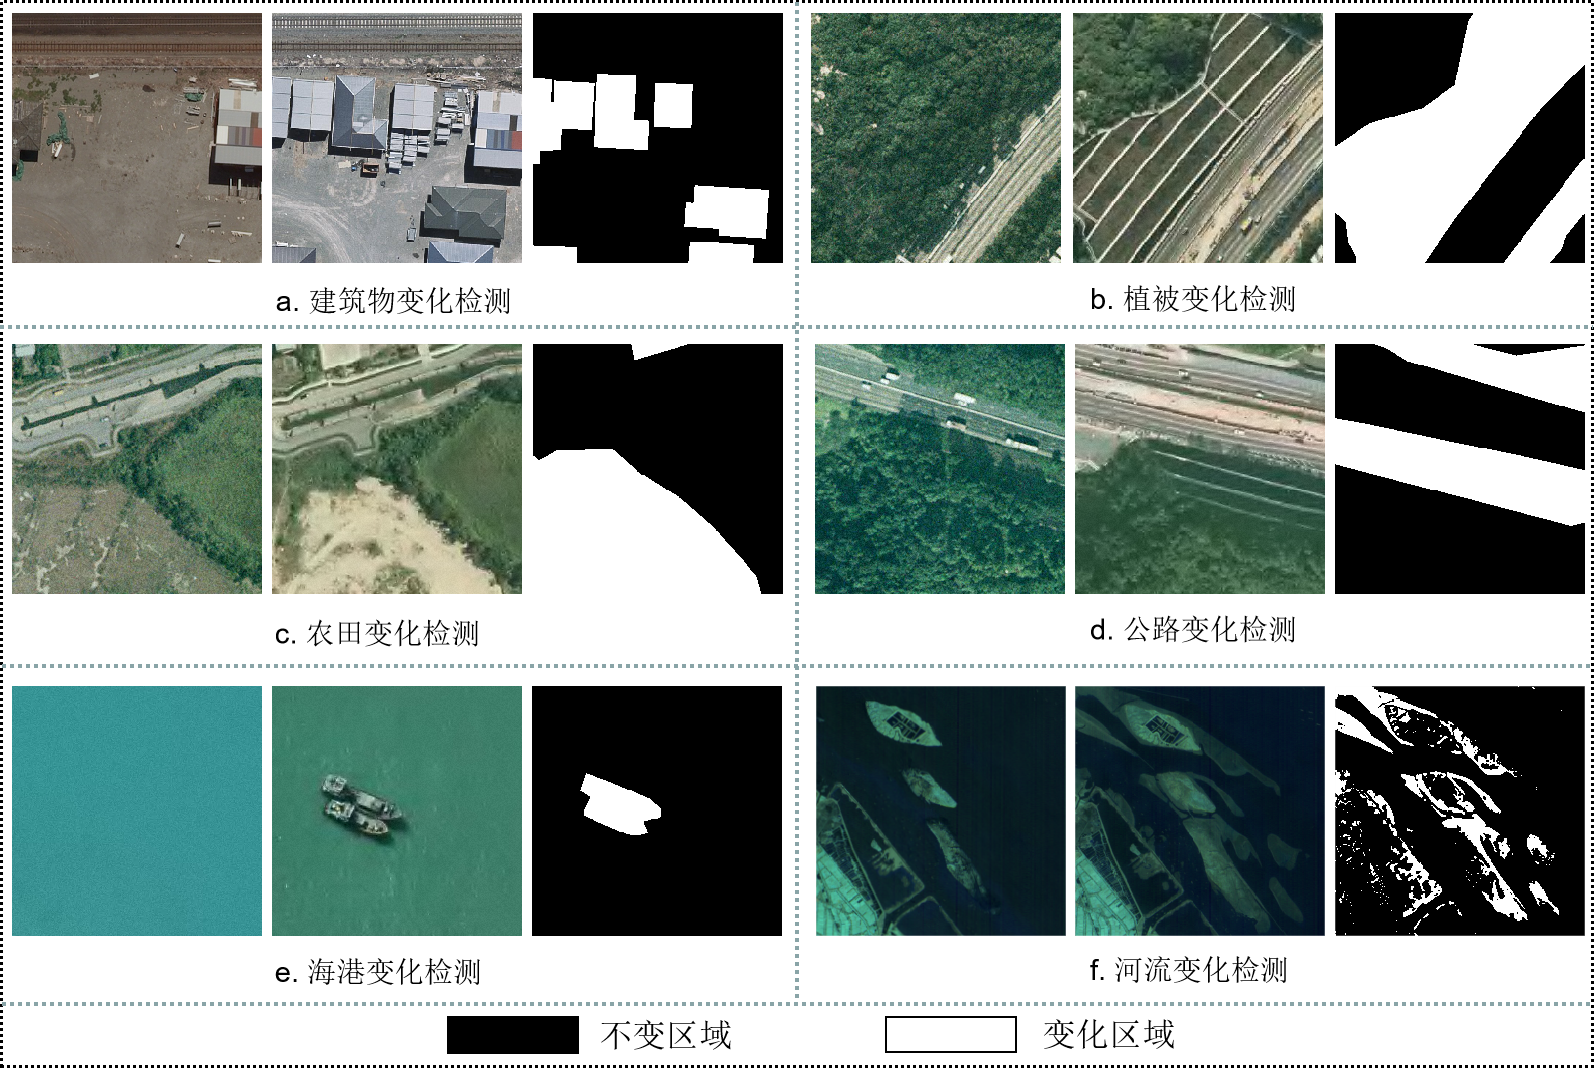
\includegraphics[scale=0.55]{images/fig1.png}
	\caption{
		各种应用领域中的变化检测
	}
	\label{fig:background}
\end{figure}

目前,深度学习算法已广泛应用于各类计算机视觉任务,例如图像分类、目标检测、单目深度估计,以及语义分割、实例分割等与变化检测相似的密集预测任务,并表现出远超传统方法的优异性能。然而,基于卷积神经网络\cite{daudt2018FC-EF}\cite{BIFA2024}\cite{crossRES2023szw}(Convolutional Neural Network, CNN)或Transformer网络\cite{chen2021BIT}\cite{Bandara2022changeformer}的全监督变化检测算法都高度依赖于大量的人工标注训练数据,当标注样本不足时,模型的检测能力会急剧下降。而变化检测任务的数据标注过程尤为复杂,需要高精度的几何图像配准和像素级的精细标注,会耗费大量时间和人力资源。这一特点导致变化检测的数据集规模远小于其他计算机视觉任务,例如图像分类、目标检测的数据集通常能够达到数十万张的规模,而公开的变化检测数据集通常仅包含几百至几万张图像样本。
为了应对上述挑战,研究人员探索了一系列方法,包括弱监督变化检测\cite{wu2023fcdgan}\cite{WSCD_TGRS24}\cite{WSCD_TGRS24_2}(Weakly Supervised Change Detection, WSCD)、无监督变化检测\cite{bandara2023USCD}\cite{USCD_JSTARS23}\cite{USCD_TGRS22}(Unsupervised Change Detection, USCD)和半监督变化检测\cite{peng2021SemiCDNet}\cite{bandara2022RCR}\cite{Zhang2023FPA}(Semi-supervised Change Detection, SSCD)。虽然弱监督变化检测具有一定的成本效益,但它同样依赖于不完整或不准确的标签,可能会引入不可预测的噪声,降低模型可靠性。另一方面,无监督变化检测不使用任何标记数据,而是利用数据中存在的固有特性进行学习,然而,在处理分类或检测等需要语义信息的任务时,存在严重的局限性。除此之外,还有一些方法采用样本生成策略,包括数据增强\cite{IAug2022}\cite{augmentaion_23}、生成对抗网络\cite{gen_sample_TGRS21}(Generative Adversarial Networks,GAN)和扩散模型\cite{bandara2022ddpm},通过模拟或合成额外的样本来提高模型性能。然而,当处理有限的可用样本时,由于生成的数据多样性不足或者与原始数据分布差异较大,这些方法可能会面临泛化能力下降的问题。相比之下,半监督变化检测提供了一种更为有效的解决方案。半监督学习\cite{Tarvainen2017teacher}\cite{ran2023DTFSeg}\cite{ran2024semi}(Semi-supervised Learning,SSL)旨在通过利用有限的可用标记样本和大量无标记样本来提升变化检测性能。通常,研究人员为无标记的数据生成伪标签,作为学习目标用于指导训练,这些伪标签通常是具有较高概率的临时预测。最广泛使用的框架是平均教师\cite{Tarvainen2017teacher}(Mean-Teacher,MT)框架,它使用教师模型来生成伪标签,并通过学生模型的指数移动平均\cite{cai2021ema}(Exponential moving average,EMA)来更新教师模型权重。受益于同时在有限的标记数据和大量无标记数据上进行训练,学生模型不仅能够学习到所需的语义信息,还能够更加充分地学习到语义特征分布,从而显著地提高模型的鲁棒性。

在此背景之下,本文着力研究了半监督变化检测算法,针对模型为无标记样本生成的伪标签可能包含错误标签和引入额外噪声的问题,提出了一系列的改进方法。具体来说,我们从以下三个方面进行了优化:首先,通过设计自适应筛选阈值和低置信度学习机制,即减少了低质量伪标签的干扰又提高了标签的利用率;其次,基于对伪标签质量的评估,进一步对其进行自适应地优化,以提升其准确性和可靠性;最后,引入自适应特征扰动一致性,减小硬伪标签固有的噪声影响,增强了模型的稳定性和泛化能力。通过这些改进,本文显著提升了半监督变化检测算法的性能。

\section{国内外研究现状及趋势}
此前,国内外学者在半监督变化检测算法领域已开展了大量研究。本小节将重点介绍与本文密切相关的三个方向的研究现状:半监督学习算法的理论与应用,基于深度学习的遥感影像变化检测技术,以及半监督遥感影像变化检测的任务特点、方法和发展历程。
\subsection{半监督学习算法}
在实际应用场景中,无标签的数据获取相对容易,而标注数据的收集通常非常困难且耗时耗力。在这种背景下,半监督学习作为一种解决样本标注困难问题的可行方法,近年来已成为深度学习领域的研究热点,其旨在仅利用一小部分标记数据进行监督训练,学习到正确的语音信息,同时利用大量的无标注训练样本进行无监督训练,以提高模型的泛化性,减少过拟合现象。SSL主要包含三种策略:一致正则化(Consistent Regularization, CR)、自训练(Self Training)、生成模型(Generative Model)以及包括其中多种思想的整体方法(Holistic Methods)。

一致性正则化方法基于平滑假设\cite{van2020smmooth}和聚类假设\cite{lee2013pseudo}的理论基础。平滑假设认为,如果两个输入样本相似,则它们的输出也应该相似。这意味着当两个输入样本属于同一类别并且位于同一个簇时,其预测输出应该相近;聚类假设提出,输入数据点倾向于形成簇,每个簇对应于一个输出类别。如果输入点位于同一个簇中,则它们可以认为属于同一类。在此基础上,低密度分离假设认为,决策边界应位于数据分布的低密度区域。因此基于这些假设,当对未标记数据施加一定程度的扰动时,其预测结果要保持稳定,即输出不应发生显著变化。

一致性正则化方法通过对输入数据施加不同程度的扰动,利用模型在这些输入数据上的输出一致性作为训练约束。目前,三种主流的一致性正则化训练框架包括:$\pi$-模型\cite{laine2016temporal}、时间集成模型\cite{laine2016temporal}和平均教师模型\cite{Tarvainen2017teacher}。这几种框架都是以孪生网络作为基础架构,两个网络分支分别处理扰动后的训练样本和原始训练样本,通过最小化两次推理概率分布的差异来优化模型。其中$\pi$-模型的两个分支网络共享参数权重,每次两个分支同步更新参数,结构简单且高效;时间集成模型通过将时间序列上的输出结果进行指数移动平均,将当前预测结果与历史预测结果结合起来,有效地保留历史了信息,减少了噪声干扰,提升了预测的稳定性;平均教师模型从模型参数层面进行平滑操作,学生模型的权重通过EMA集成了历史模型参数。其中平均教师模型被广泛应用于各个领域的半监督研究,例如半监督目标检测算法Active-Teacher\cite{ActiveTeacher},半监督语义分割算法\cite{mittal2019s4GAN}\cite{UniMatch}\cite{AugSeg}\cite{iMAS},半监督图像分类算法\cite{sohn2020fixmatch},半监督医学图像分割算法\cite{transformation_medical}\cite{zhangSemiSAMExploringSAM2023}。
此外基于此框架,一些研究人员也在扰动设计方面进行了探索,比如Xie等人\cite{xie2020unsupervised}和Bandara等人\cite{bandara2022RCR}分别在一致性正则化中应用了图像级扰动和特征级扰动,这些研究从不同维度丰富了基于一致性正则化的半监督方法。

基于自训练的半监督学习算法的核心思想是:首先使利用预测模型或其变体为无标记样本生成伪标签,将这些无标记样本以及伪标签与标记训练样本混合,一起进行监督训练,从而为模型提供扩充的训练数据。然而,一个最为关键的问题就在于伪标签的可靠性,这将直接影响模型的训练效果,因此大量的研究集中于如何生成高质量的伪标签。Lai等人\cite{Lai2021CAC}提出采用一个设定的概率阈值作为选择标准,仅保留预测概率高于该阈值的标签,过滤掉低置信的伪标签。ST++\cite{yang2022st++}设计了一种多层自训练结构,每个阶段选择一批高质量的伪标签参与训练,通过多轮“选择-训练”循环,直到所有未标记的样本都得到了利用。U2PL\cite{wang2022u2pl}通过计算伪标签中每个像素的信息熵,使用恒定的熵值作为过滤阈值,过滤掉低熵(高不确定性)的伪标签。此外还有一种协同训练(Co-training)框架\cite{co-training},这种框架采用两个独立模型,分别为对方提供伪标签,通过两个模型之间的互补性来提高伪标签的可靠性,同时减少但模型可能存在的偏差。

基于生成模型的方法旨在利用生成模型对数据的分布进行建模,从而推断出未标注数据的潜在信息。其中,半监督变分自编码器\cite{semiVAE}(Semi-supervised Variational Autoencoder, Semi-VAE)是一种将变分自编码器(Variational Autoencoder, VAE)扩展到半监督学习的创新方法,通过添加一个分类器来学习语义信息,首先从标注样本集中学习真实的数据分布,然后基于分类器对无标注样本的分类结果,指导模型学习一个更为丰富的潜在分布。Ren等人\cite{gen_sample_TGRS21}提出了一种基于生成对抗网络的方法,利用生成对抗策略训练了一个能够生成共配准图像的生成器。具体来说,首先在原始图像高维特征空间中采样,并从特征空间分布的上界和下界之间按照策略选择一些特征向量生成高质量配准图像。随后,通过特征融合提取变化区域,扩充了模型可学习的特征空间。此外,Bandara等人\cite{bandara2022ddpm}在大规模数据集上预训练了一个去噪扩散概率模型(Denoising Diffusion Probabilistic Models,DDPM),利用其具有强大表征能力的编码器进行双时图像的特征提取以提高变化检测性能。

在实际应用中,更多被采用的是整体方法,即在一个框架中整合前述多种半监督学习策略,从而实现更高的性能。其中,最为经典的方法之一是FixMatch\cite{sohn2020fixmatch},其结合了伪标签自训练和一致性正则化,提出了一种简单而高效的框架。进一步,Yang等人\cite{UniMatch}针对分类和分割任务的特点差异,引入了一种新的特征扰动前馈输入流和一个额外的强增强扰动输入流,通过多重一致性约束构造更广阔的扰动空间。此外,Yang等人在半监督语义分割领域还提出了两项具有意义的研究\cite{AugSeg}\cite{iMAS},他们在训练中加入了自适应图像增强机制,有效地提升了模型在处理复杂语义分割任务时的性能,这些研究不仅为整体方法的进一步优化提高了参考,也启发了本文对半监督变化检测算法的研究,尤其是在结合特征扰动和设计自适应机制来提升模型性能方面提供了思路。

\subsection{基于深度学习的遥感影像变化检测算法}
受深度学习在各领域取得巨大成功的启发,过去十年中,变化检测领域涌现出一系列经典研究,极大地推动了遥感影像变化检测的发展。本小节将大致按照时间顺序分别介绍相关技术,包括基于卷积神经网络的变化检测方法、基于Transformer的变化检测方法以及近期兴起的基于大模型的变化检测方法。
\subsubsection{基于CNN的变化检测算法}
CNN通过引入卷积和池化操作,能够有效地捕获图像的空间特征和局部关系,同时深度网络结构可以逐层提取更抽象的高维特征。经典的CNN架构包括LeNet-5\cite{lecun1998lenet}、AlexNet\cite{krizhevsky2012alexnet}、VGGNet\cite{simonyan2014VGG}、ResNet\cite{He2015ResNet}以及UNet\cite{ronneberger2015Unet}等。在变化检测中,研究人员通常利用双分支孪生网络分别处理两幅时相图像,提取高维特征后进行特征融合,从而识别出双时相图像对之间的差异。最为经典的工作是Daudt 等人\cite{daudt2018FC-EF}使用全卷积网络构建了基于UNet的变化检测框架及其两个孪生变体,这三种变化检测框架分别是FC-EF、FC-Siam-conc、FC-Siam-diff,每种框架都采用了不同的特征融合策略,其中FC-EF是在输入层面首先对双时相图像进行了图像级别的融合,另外两种都是对从双时相图像对中抽取的高维特征进行融合。Shi等人\cite{shi2021DSAMNet}提出的DSAMNet在每个多尺度特征融合阶段添加了卷积块注意模块\cite{woo2018cbam}(Convolutional Block Attention Modules,CBAM),这种轻量级的注意力机制从空间和通道两个维度上对特征之间的关系进行了建模,动态地调整了特征图的权重。Zhang等人\cite{zhang2023MFNet}提出了一个互特征学习网络——MFNet(Mutual Feature-Aware Networks),设计了对称变化特征融合模块,有效地解决了差分特征融合造成的信息丢失问题。同时通过在编码阶段提前引入差异感知,使得编码器更加聚焦于对潜在变化区域的特征学习。Fang等人\cite{fang2021SNUNet}将孪生网络和稠密连接的NestedUNet网络\cite{zhou2018unet++}结合,通过紧凑的信息传输减少浅层特征和深层特征之间的位置信息丢失。Zheng等人提出的ChangeStar\cite{zheng2021changestar}通过构造伪配准图像对,以语义分割方式来处理两幅图像,以单时相图像来训练双时相图像对变化检测模型,减少了对特征融合和图像配准的依赖。总的来说,基于CNN的监督变化检测方法大多侧重于特征融合模块或者精巧的编码器设计,致力于更加精确地表示变化特征。
\subsubsection{基于Transformer的变化检测算法}
Transformer 是一种基于自注意力机制的深度学习模型,由 Vaswani 等人\cite{vaswani2017transformer}在 2017 年首次提出,并在自然语言处理任务中取得了革命性突破,尤其在机器翻译任务中的序列到序列(Seq2Seq)建模方面表现卓越。其核心特性是完全摒弃了传统的循环神经网络\cite{zaremba2014rnn}(Recurrent Neural Network,RNN)和卷积神经网络,以自注意力机制和全连接网络为基础,显著提升了模型在长程依赖任务中的效率和性能。随着Google Research 于 2020 年提出了Vision Transformer (ViT)\cite{dosovitskiy2020vit},首次将Transformer网络应引入了计算机视觉领域,并迅速成为了该领域的研究热点,ViT的成功为变化检测开辟了新的研究方向,许多基于Transformer的变化检测方法应运而生。Chen等人首先将ViT引入了变化检测任务,提出了基于原生 Transformer 架构的变化检测模型BIT\cite{chen2021BIT},该模型通过Transformer对双时相图像的时空上下文进行建模,取得了初步成果。然而,由于直接采用原生 Transformer 解码器,未能充分利用浅层特征,这限制了其性能。在此基础之上,Li 等人提出了TransUnet\cite{li2022transunetcd},使用UNet 风格的解码器取代了 Transformer 原有的解码方式,在解码过程中融合上一阶段的特征图逐步恢复至原始尺寸,从而显著提升了模型的表现。受语义分割网络SegFormer \cite{xie2021segformer}的启发,Bandara 等人设计了用于变化检测的 ChangeFormer\cite{bandara2022transformer},该模型通过卷积操作学习双时相特征图之间的变化关系,展现了比之前纯Transformer模型更高的精度和鲁棒性。Jiang等人提出的VcT\cite{jiang2023vct}引入了图神经网络(Graph Neural Network, GNN),将每个像素视为图节点,利用节点间的结构化信息建模变化特征。与以往固定token的方式相比,VcT通过动态挖掘共享背景信息的可靠token,提高了检测效率和准确性。

一些研究发现,由于变化检测任务中的训练数据量通常有限,纯Transformer模型可能无法充分发挥其潜力。因此还有一些研究将CNN和Transformer结合在了一起,这类方法旨在利用CNN强大的局部特征捕捉能力,同时发挥Transformer在全局特征建模中的优势,从而实现全局与局部特征学习的统一。比较经典的工作有Jiang提出的MSFCTNet\cite{jiang2024cnntranscd}和Li等提出的MCTNet\cite{lwm2023cnntransCD2}和ConvTransNet\cite{lwm2023cnntransCD}。总体来看,这些方法通过创新性的架构设计,从不同角度实现了CNN和Transformer特征的高效融合,弥补了单一模型的局限性,为变化检测任务提供了更精确的特征表示和更强的鲁棒性。
\subsubsection{基于大模型的变化检测算法}
近年来,大模型(Large Models)的发展成为人工智能领域的核心热点之一。这些模型以大规模参数、海量数据和复杂架构为特征,在自然语言处理、计算机视觉、强化学习等领域展现出卓越的性能。它们通常基于自注意力机制(Self-Attention)驱动的Transformer模型,通过在大规模数据集上的自监督预训练,获得了强大的通用表征提取能力。尽管大模型与上一小节讨论的Transformer模型在技术上具有相似性,但由于其规模和性能的突破性提升,已引发了多领域的变革。本小节将单独分析基于大模型的变化检测研究。自从自然语言处理领域大模型(如BERT、GPT)问世以来,预训练大模型的概念迅速扩展到计算机视觉领域,随着模型参数规模的增加,计算机视觉预训练模型在提取视觉特征、建模全局关系和提升任务鲁棒性方面表现出了显著优势,为变化检测任务带来了全新的解决方案。其中,SAM\cite{kirillov2023SAM}(Segment Anything Model)作为图像分割通用大模型的开篇之作,以其强大的零样本推理能力和无需微调的交互式分割,颠覆了传统的深度学习方法,为变化检测提供了重要启发。Li等人\cite{li2024LM}最早提出了结合大模型进行变化检测的新范式,设计了双时态适配网络(BAN),由冻结的基础模型(如CLIP\cite{radford2021clip}、SAM)、双时态适配分支(Bi-TAB)以及它们之间的桥接模块组成。该方法将大模型的丰富先验知识注入到了变化检测模型,有效提升了模型的泛化性能。Ding等人\cite{ding2024SAMCD}通过训练一个轻量级的适配器网络(Adapter),针对遥感影像场景性优化了SAM的视觉表示能力,以更精确地提取双时相图像的特征。Liu等人\cite{liu2024changeagent}提出了变化检测智能体(Change-Agent),结合大语言模型(Large Language Model,LLM)和变化检测模型结合起来,能够处理文本和图像两种模态数据,按照输入指令交互式地检测感兴趣的变化区域。Dong等人\cite{dong2024changeclip}基于CLIP设计了多模态变化检测模型,通过结合图像-文本的编码结果与解码阶段的视觉特征,增强了变化检测的语义表征能力。Zheng等人\cite{zheng2024SAC}提出了一种基于SAM的零样本变化检测方法,通过构建点提示并利用SAM提取的特征空间,挖掘图像内和图像间的潜在相似性。这种方法无需额外训练模型即可实现推理,但仍需要对每幅图像进行人工点提示标注,与传统意义上的零样本任务有所不同。

基于大模型的变化检测方法展示了强大的潜力,包括丰富的先验知识、跨模态处理能力以及高效的零样本推理。然而,这些方法在标注需求、适配器设计以及推理效率等方面仍存在挑战。未来,如何进一步优化大模型在变化检测中的适用性将成为重要研究方向。
\subsection{半监督遥感影像变化检测算法}
由于对大量图像进行变化检测任务的精细标注耗时且成本高昂,半监督变化检测成为解决此问题的主要方法。与第1.2.1小节中提到的半监督学习算法类似,SSCD也主要分为两大类别,其一是基于CR的方法,其二是基于GAN的方法。

在一致性正则化方面,Bousias等人\cite{bousias2021evaluation}的最早将平均教师模型引入变化检测任务中。然而,这一尝试在初始的实验结果中并未表现出显著的潜力,与仅使用有限数量的标记数据进行全监督学习的基准相比,这种SSCD方法存在不足,甚至随着真实标注数据增加,这种与全监督训练之间的性能差距进一步扩大。Mao等人\cite{mao2023semi}做出了一些改进,分别对教师模型和学生模型的输入进行了强、弱增强操作。此外,他们制定了一个额外的教师虚拟对抗训练组件,以进一步减少伪标签噪音的负面影响。Sun等\cite{sun2022semisanet}结合了额外的基于伪标签自训练框架,并在孪生网络中结合阈值过滤机制,用以移除低质量伪标签。通过降低低置信度伪标签的干扰,该方法有效减少了伪标签噪声对自训练的不利影响。Hafner等人\cite{hafner2022urban}提出了一种双任务SSCD框架,该框架结合了建筑物分割和变化检测这两个密切相关的下游任务。通过在孪生分割网络和变化检测网络产生的两个变化检测掩码之间施加一致性约束,提升了模型的性能。Bandara等\cite{bandara2022RCR}探索了新的正则化项,即基于特征的扰动,通过在特征层面应用各种数据扰动,扩展一致性约束的分布空间。该方法充分利用了未标记样本中嵌入的信息。在最近的工作中,Zhang等人\cite{Zhang2023FPA}提出了一种类一致性和特征一致性联合约束方法,通过对未标记样本的变化类和不变类特征表示进行对齐,模型得以从更接近真实分布的特征空间中学习,从而显著提升了SSCD的性能。

其他方法主要基于GAN这种生成模型,其最初由Goodfellow在2014年提出\cite{goodfellow2014gan}。其中一些研究利用GAN来学习接近真实标记数据的特征分布空间\cite{peng2021SemiCDNet}\cite{graph2019gan}\cite{nie2022semigan}\cite{yang2022gan};另一部分研究将GAN用于生成数据样本\cite{li2023multi}\cite{gen_sample_TGRS21};在最近的工作中,Wu等人\cite{wu2023fcdgan}提出了一种新的变化检测范式,将无监督、弱监督、区域监督和完全监督的变化检测任务统一到一个端到端框架中。该方法通过生成对抗网络(GAN)实现对多种监督模式的适配,在变化检测领域具有重要创新意义。在无监督变化检测任务中,该方法的主要目标是最小化一个区域,使得生成网络在屏蔽该区域后之后,生成与另一时相图像相似的图像,从而从无标记图像对中学习到知识。对于弱监督和新提出的区域监督变化检测任务,方法的关键思想在于最小化一个区域,使判别网络在屏蔽该区域后无法区分真实的不变图像对。这种设计通过对生成器和判别器的协同优化,提高了模型对复杂变化区域的检测能力。虽然以上这些方法在SSCD中取得了一定成功,但仍存在一些挑战:GAN的训练过程高度不稳定,使得超参数调整变得复杂且耗时;在训练阶段,梯度消失问题常导致生成器难以持续优化;若未引入额外的正则化策略,鉴别器的强判别能力可能导致GAN的生成器和鉴别器之间的性能不平衡,从而抑制生成器的学习能力。因此,达到理想的最优训练结果是难以实现的,这使得该类方法的实际应用场景比较局限。
\section{本文主要内容及结构安排}
本文着力研究半监督变化检测任务,在少量有标注训练数据上学习正确的语义信息并在大量且易获得的无标注训练样本上学习到一个更加丰富的特征空间分布。其中一个关键问题就在于能否减少无标注样本训练中不可避免的噪声问题,这有两种解决方案:通过改善伪标签的质量来提高半监督变化检测的性能;从特征层面构造正则化项从而排除错误伪标签的重要影响。本文从这两点入手,研究内容和论文组织结构的对应关系如图\ref{fig:paper_frame}所示,其中主要研究内容如下:

1)基于自适应动态阈值半监督变化检测。针对此前基于一致性正则化和自训练的变化检测算法中,使用固定阈值或者固定阈值调整方案筛选伪标签导致的无标记训练数据利用率低下的问题,我们提出了一种根据模型的学习状态自适应调整阈值的半监督变化检测算法,首先根据全局预测置信度随着训练进程自适应地增大整体阈值,并根据前景、背景类别置信度为两个类别分配更加精确的阈值,最后对于被筛选掉的标签,通过低置信度学习模块,将其纳入模型训练之中,进一步提高训练样本利用率。实验表明我们提出的自适应阈值相比此前半监督变化检测中采用的阈值筛选方案,能够达到更好的变化检测性能。

2)基于自适应伪标签优化的半监督变化检测。针对大量的无标注样本中不同样本个体之间存在很大的差异,模型为这些具有不同难易程度的样本生成的伪标签可靠性也不尽相同。本算法设计了一种自适应动态学习策略AdaSemiCD,旨在从样本和模型两个层面对伪标签生成进行优化。我们的框架结合了传统的半监督训练方法,并辅以两个创新的功能模块AdaFusion和AdaEMA。首先,我们利用AdaFusion在单个样本水平上对不确定性高的样本区域进行改造,从而提高伪标签的准确性。其次在AdaEMA模块中引入了模型级参数更新的自适应选择过程,使模型能够充分集成优越的参数。大量的实验结果表明了我们所提出的方法能够极大地改善伪标签的质量,使得变化检测性能更好。
\begin{figure}[H]
  \centering
  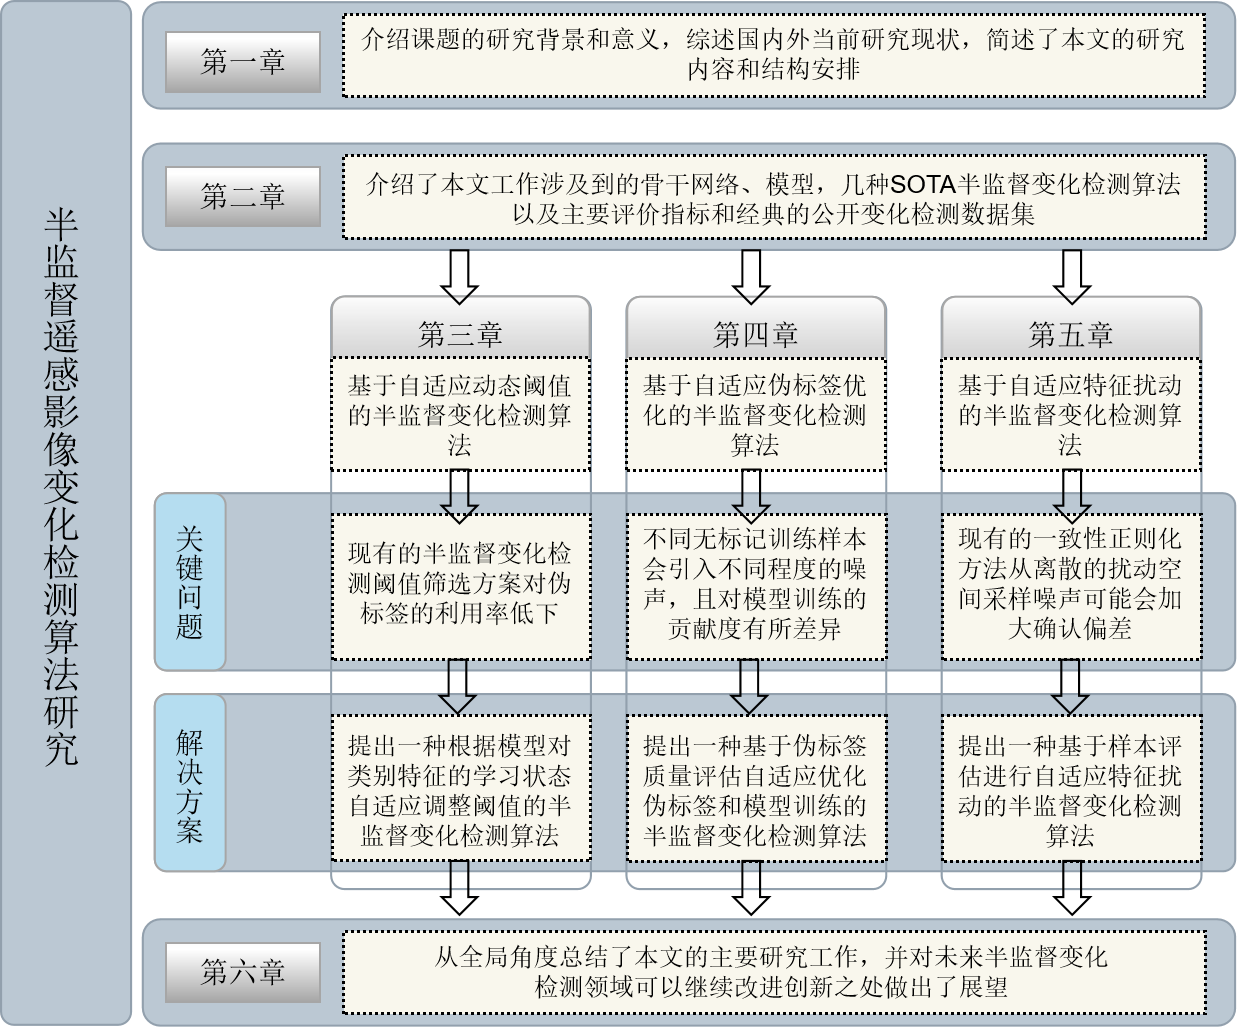
\includegraphics[scale=0.75]{images/paper_frame.png}
  \caption{
    本文研究内容和组织结构对应关系图
  }
  \label{fig:paper_frame}
\end{figure}

3)基于自适应特征扰动的半监督变化检测。针对可能对半监督学习的一致性原理和边缘假设造成挑战的两个问题:(1)模型对未标记图像的预测并不总是足够准确的;(2)对无标记图像施加的扰动并不总是对模型训练有效的。我们提出了一种根据样本质量进行自适应特征扰动的半监督变化检测算法,首先利用概率分布的对其替换单一硬标签
学习,从而缓和伪标签的不确定性,并提高对软标签信息的利用;其次我们针对不同样本进行自适应地特征扰动,在随机扰动地基础上实现了一定的可控性,减少了模型的确认偏差。最后进行了大量的实验,验证了我们的设想的正确性和改进措施的有效性。

全文包括六章,具体的章节结构安排如下:

第一章首先系统性地阐述了变化检测任务的应用场景和研究价值,以及半监督变化检测算法的研究背景和意义,然后梳理了目前国内外关于半监督学习、深度变化检测、半监督变化检测的研究进展和主流方法,最后介绍了本文的主要研究内容和文章结构安排。

第二章首先介绍了本文研究工作中用到的一些骨干特征提取网络,之后对本研究工作中进行对比的几种经典半监督变化检测算法进行了阐述,最后详细介绍了本研究中采用的实验指标和用到的数据集。

第三章基于自适应动态阈值的半监督变化检测工作介绍。首先整体性的阐述了算法的框架和训练流程,随后详细介绍了基于预测概率分布的全局动态阈值和类别动态阈值,以及设计的低置信度学习模块。最后在实验部分报告了本章方法在十个公开数据集上取得的实验结果,从定性和定量两个角度进行了全方位的对比,以及全面的消融实验
分析,验证了该工作的有效性。

第四章基于伪标签评估的自适应半监督变化检测工作介绍。首先介绍了模型的整体框架以及训练流程,随后详细介绍了设计的伪标签评估指标,以及基于此指标设计的两个自适应模块。最后在实验部分报告了该研究方法在十个公开数据集上取得的实验结果,并与其他经典半监督变化检测算法在定性和定量上进行了公平的对比,最后通过消融实验证明了每个模块的有效性。

第五章基于自适应特征扰动的半监督变化检测工作介绍,首先从全局角度阐述了算法的框架和流程,随后具体地介绍了我们设计的基于无标记样本预测评估的自适应特征扰动方法。最后在实验部分报告了我们在十个公开数据集上对本章方法进行实验验证取得的实验结果,包括定量实验指标和定性可视分析,此外还对本章提出的自适应扰动模块进行了消融分析,证明了本章研究的有效性。

第六章总结与展望。从全局角度总结了本文的主要研究工作,并对未来半监督变化检测领域可以继续改进创新之处做出了展望。
\chapter{相关技术}

本章将介绍本文基于深度学习的半监督变化检测算法研究所涉及的相关技术,为后续章节提供技术背景支持。具体包括:2.1小节中详细介绍本文几个研究工作中用到的深度神经网络,包括卷积神经网络,Vision Transformer的网络结构以及平均教师框架等;2.2小节对上一章节研究现状中概括性介绍的几个经典半监督变化检测算法进行了详细的阐述;2.3小节对本文所有实验所采用的实验指标进行了解释;2.4小节对本文所有进行实验的公开数据集进行了详细介绍。

\section{深度神经网络}
深度神经网络是一种以多层神经元结构为基础的机器学习模型,广泛应用于诸多领域,包括计算机视觉、自然语言处理、语音识别以及推荐系统等。基于任务需求,衍生出了多种具体架构,例如用于图像处理的卷积神经网络CNN,在序列建模中表现优异的循环神经网络RNN,以及基于多头自注意力机制对全局关系进行建模的Transformer架构。虽然神经网络并不是本文的主要研究方向,但是由于后续研究中会多次涉及卷积神经网络中比较经典的网络模型,因此在本小节将介绍后续研究工作所用到的几种骨干特征提取网络,即ResNet,Vision Transformer,以及基于Transformer预训练的通用分割大模型Segment Anything Model的模型结构。
\subsection{ResNet}
在深度学习的发展过程中,研究者们发现随着卷积神经网络层数的增加,模型的表达能力理论上会不断增强。然而,在实际训练深层网络时,却遇到了两个主要问题:(1)梯度消失和梯度爆炸问题;(2)退化问题。这些问题阻碍了深层神经网络的发展,最终何等人\cite{He2015ResNet}提出了残差网络(Residual Network, ResNet),通过在网络层之间引入残差连接使得前层的输出直接加到后层的输出上,如公式\ref{eq:resnet}所示,其中$x$代表输入特征,下标表示网络层序号,$W_l$代表第$l$层的参数,$F\left(x_l,W_l\right)$表示卷积映射。通过这种方式,梯度在反向传播时可以通过跳跃路径直接传播到前层,避免了梯度逐层递减的问题,从而缓解了梯度消失,同时即使一些层对学习贡献较小,残差连接可以保证网络的性能至少不会发生退化现象。
\begin{equation}
  \label{eq:resnet}
  x_{l+1} = x_l + F\left(x_l,W_l\right)
\end{equation}

此外残差结构还减少了优化深层网络的难度,是网络结构更加复杂、网络层数进一步增加成为了可能,从而显著提升了卷积神经网络的表征能力和性能,推动了深度学习向更深、更强的方向发展。比如何等人同时提出了具有不同网络层数的ResNet,包括ResNet-18、ResNet-34、ResNet-50、ResNet-101以及ResNet-152,它们的网络架构如图\ref{fig:resnet}所示。
\begin{figure}[htb]
  \centering
  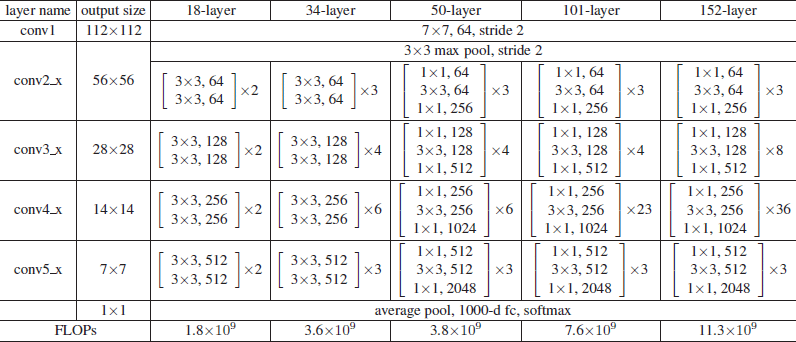
\includegraphics[scale=0.55]{images/resnet.png}
  \caption{
    不同深度的ResNet网络层次架构\cite{He2015ResNet}
  }
  \label{fig:resnet}
\end{figure}
此外后续还有研究提出了一些ResNet变体,例如ResNetV2\cite{2019resnetV2}和ResNeXt\cite{xie2017ResNeXt}。根据网络深度和任务需求,ResNet中存在两种经典的残差块,一种是用于浅层网络(如ResNet-18和ResNet-34)的基本残差块(Basic Residual Block),包含两个$ 3\times3 $的卷积层和直接的跳跃连接,一种是用于深层网络(如ResNet-50、ResNet-101和ResNet-152)的瓶颈残差块(Bottleneck Residual Block),它将两个 $ 3\times3 $ 的卷积层替换为$1 \times 1$,$3 \times 3$,$1 \times 1$ 的卷积网络,其中前后两个$1 \times 1$卷积层分别用于降低和恢复特征通道数,有效地减少了计算量和参数量,网络结构如图\ref{fig:resblock}所示。本文研究工作中采用的是ResNet-50,一共包含4个卷积阶段,每一个阶段中分别有3,4,6,3个瓶颈残差块。


\begin{figure}[htb]
  \centering
  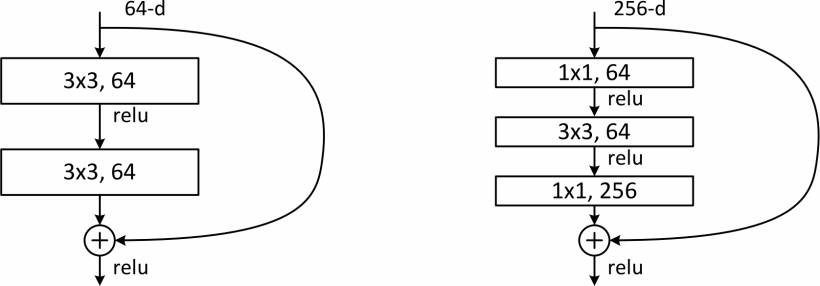
\includegraphics[scale=0.55]{images/res-block.png}
  \caption{
    两种残差块的网络结构\cite{He2015ResNet}
  }
  \label{fig:resblock}
\end{figure}

\subsection{Vision Transformer}
虽然CNN在计算机视觉任务(如图像分类、目标检测、语义分割等)中占据主导地位,然而其在捕捉长距离依赖和全局信息时存在很大局限性。与此同时,Transformer在自然语言处理(Natural Language Processing, NLP)领域取得了显著成功,尤其是在任务如机器翻译和文本生成中。Transformer的核心优势是通过自注意力机制(Self-Attention Mechanism)捕捉输入数据中全局依赖关系。受此启发,Dosovitskiy等人\cite{dosovitskiy2020vit}对Transformer进行改进使其能够适配计算机视觉任务,形成了Vision Transformer(ViT)架构。这种方法首次完全摆脱了卷积操作,在多个基准测试中展现出与甚至超越CNN的性能。它的核心思想是将图像分割为固定大小的图像块(patches),并将每个块视为一个独立的“词”,类似于NLP中的词嵌入,这些图像块嵌入向量通过Transformer的自注意力机制进行处理,从而实现对图像的全局理解。
\begin{figure}[htb]
  \centering
  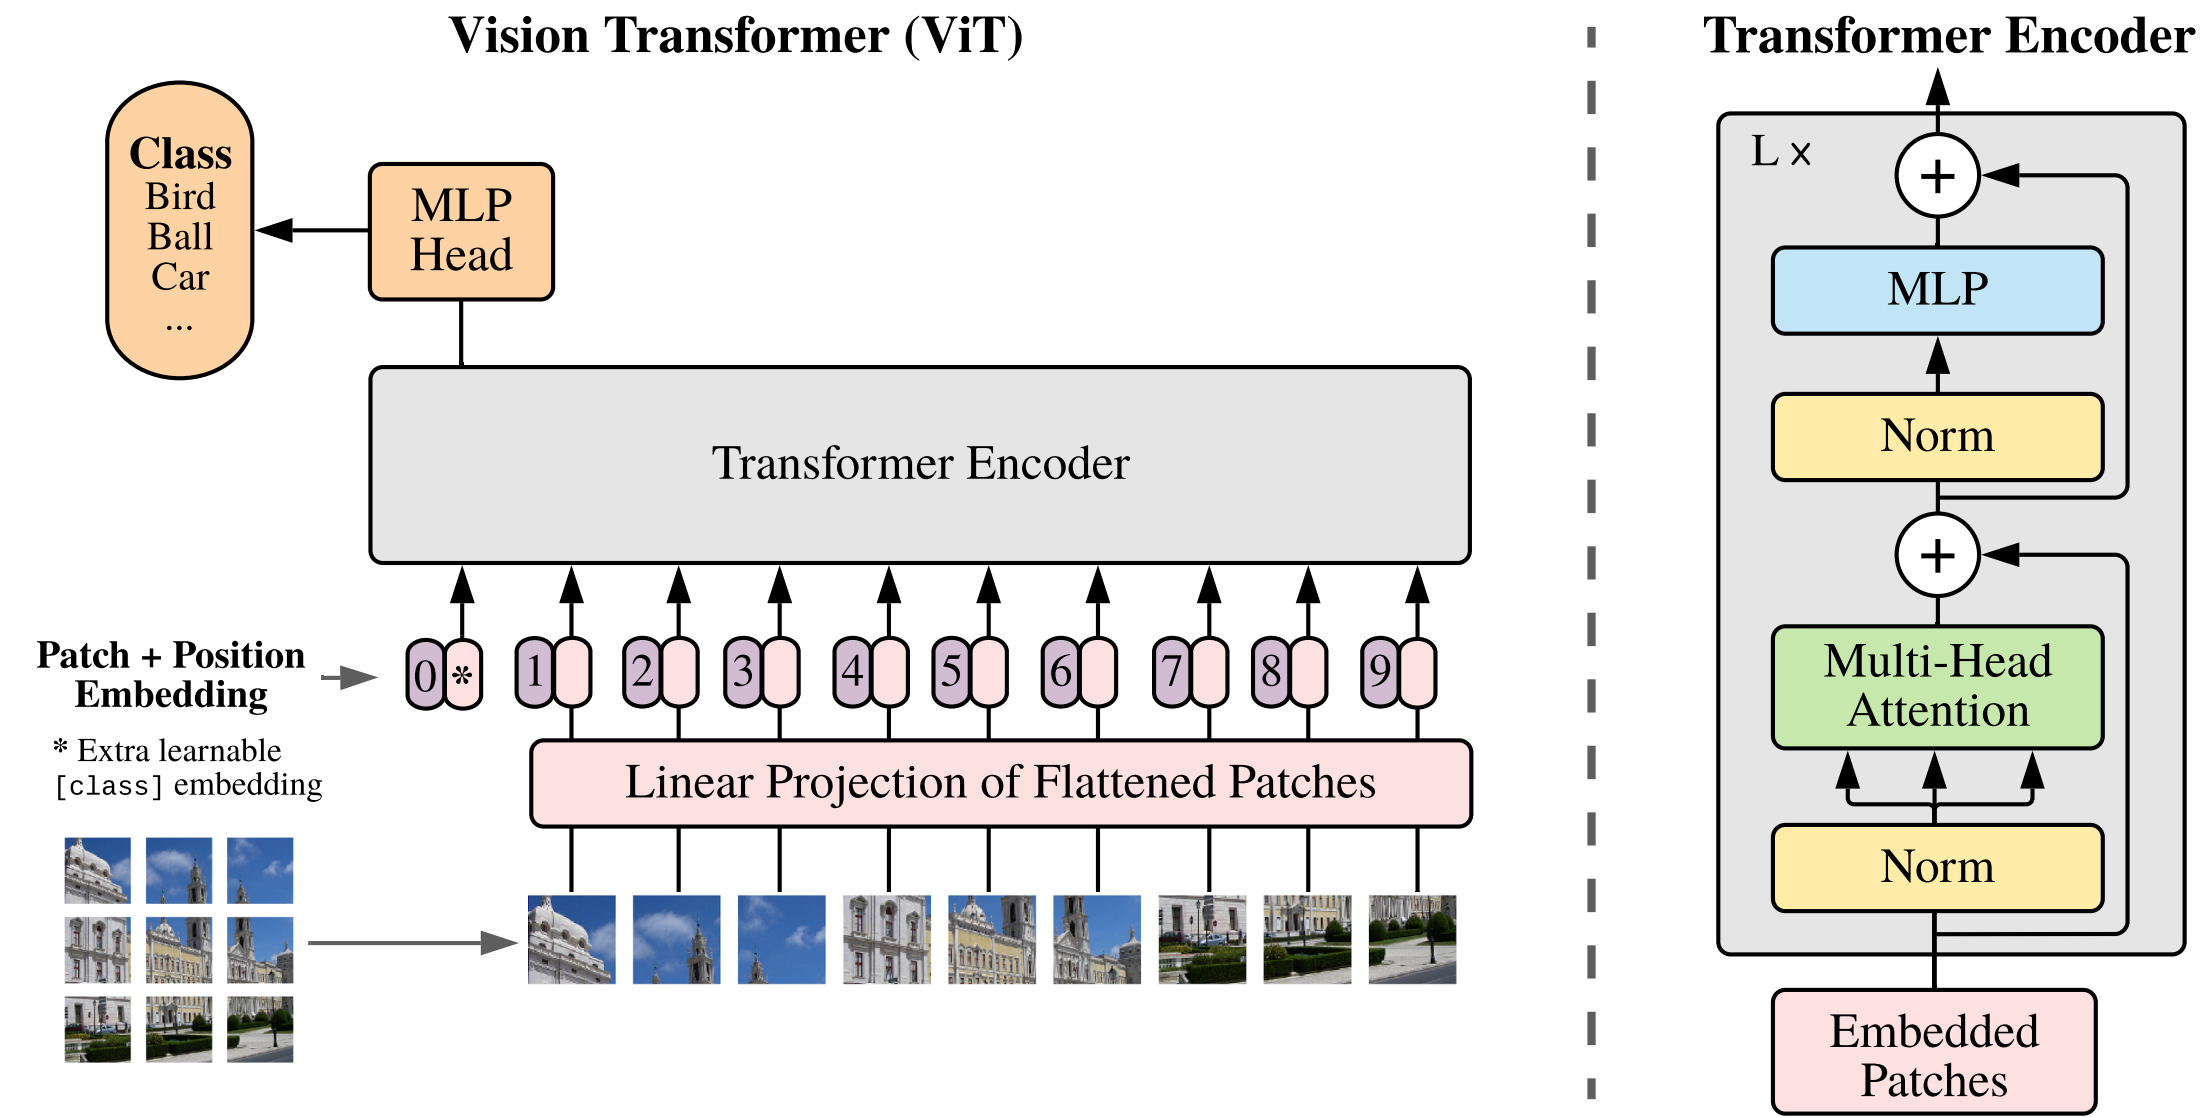
\includegraphics[scale=0.55]{images/ViT.png}
  \caption{
    Vision Transformer网络框架\cite{dosovitskiy2020vit}
  }
  \label{fig:ViT}
\end{figure}

ViT的网络结构如图\ref{fig:ViT}所示,输入的图像首先被分割为大小为$P\times P$的非重叠图像块(patches),每个块展平为一维向量并通过线性映射嵌入到D维特征空间,假设图像大小为$H \times W$且通道数为$C$,则切割后共生成$N=\frac{H}{P} \times \frac{W}{P}$个图像块,这些块被视为Transformer的输入“词”。为保留块之间的空间顺序信息,ViT为每个嵌入向量添加一个可学习的位置编码,此外,在输入序列的起始位置插入一个特殊的分类标识符([CLS] Token),该标识符的嵌入向量用于最终的分类输出,如公式\ref{eq:embeding}。经过嵌入和位置编码后的输入序列被送入由L层组成的Transformer编码器,每层包含多头自注意力机制(Multi-Head Self-Attention, MHSA)和前馈网络(Feed-Forward Network, FFN)。在MHSA中,每个图像块嵌入向量通过查询(Query)、键(Key)和值(Value)矩阵生成注意力权重,用以捕捉图像块间的全局关系,表示为公式\ref{eq:attention}。其中$Q$、$K$、$V$是从输入嵌入计算得到的查询、键和值矩阵,$\sqrt{d_{k}}$是注意力头的维度。每个Transformer层都配有残差连接和层归一化,用以提高训练稳定性。经过L层编码器后,分类标识符的嵌入向量$z_{0}^{[C L S]}$被用作图像的全局表示,并通过一个全连接层映射到类别数的维度,最终通过Softmax函数生成分类概率,如\autoref{eq:softmax},其中$W_{\text {head }}$和$b_{\text {head }}$为分类头的参数。
\begin{equation}
  \label{eq:embeding}
  z_{0}=\left[z_{0}^{[C L S]} ; z_{0}^{1} ; z_{0}^{2} ; \ldots ; z_{0}^{N}\right]+E_{\mathrm{pos}},
\end{equation}
\begin{equation}
  \label{eq:attention}
\operatorname{Attention}(Q, K, V)=\operatorname{softmax}\left(\frac{Q K^{\top}}{\sqrt{d_{k}}}\right) V,
\end{equation}
\begin{equation}
  \label{eq:softmax}
  \hat{y}=\operatorname{Softmax}\left(z_{L}^{[C L S]} W_{\text {head }}+b_{\text {head }}\right)
\end{equation}

ViT摒弃了传统卷积操作,采用自注意力机制实现图像全局特征的高效建模,其模块化和可扩展的架构使其在大规模数据集和高效计算资源支持下展现出优异性能。然而,ViT在小规模数据场景中仍面临一定挑战,主要体现在模型对训练数据的需求较高和计算效率的限制。因此,针对训练数据稀缺的情况,结合半监督学习算法是一种具有潜力的研究方向,通过充分利用未标注数据,有望显著提升ViT在小数据集场景下的表现。
\subsection{金字塔池化模型}
在传统的卷积神经网络(CNN)中,特征图的尺寸通常会随着卷积层的增加而逐渐减小。这对于处理不同尺寸的输入图像可能会带来问题,因为图像的空间信息可能在池化的过程中丢失。尤其是在语义分割、目标检测等任务中,捕捉多尺度的上下文信息对于提升模型性能至关重要。
为了更好地捕捉图像的多尺度信息,金字塔池化模型(Pyramid Pooling Module,PPM)通过对特征图进行不同尺度的池化操作,避免了仅依赖单一尺度的局限性,增强了网络对多种尺度物体的感知能力。
\begin{figure}[htb]
  \centering
  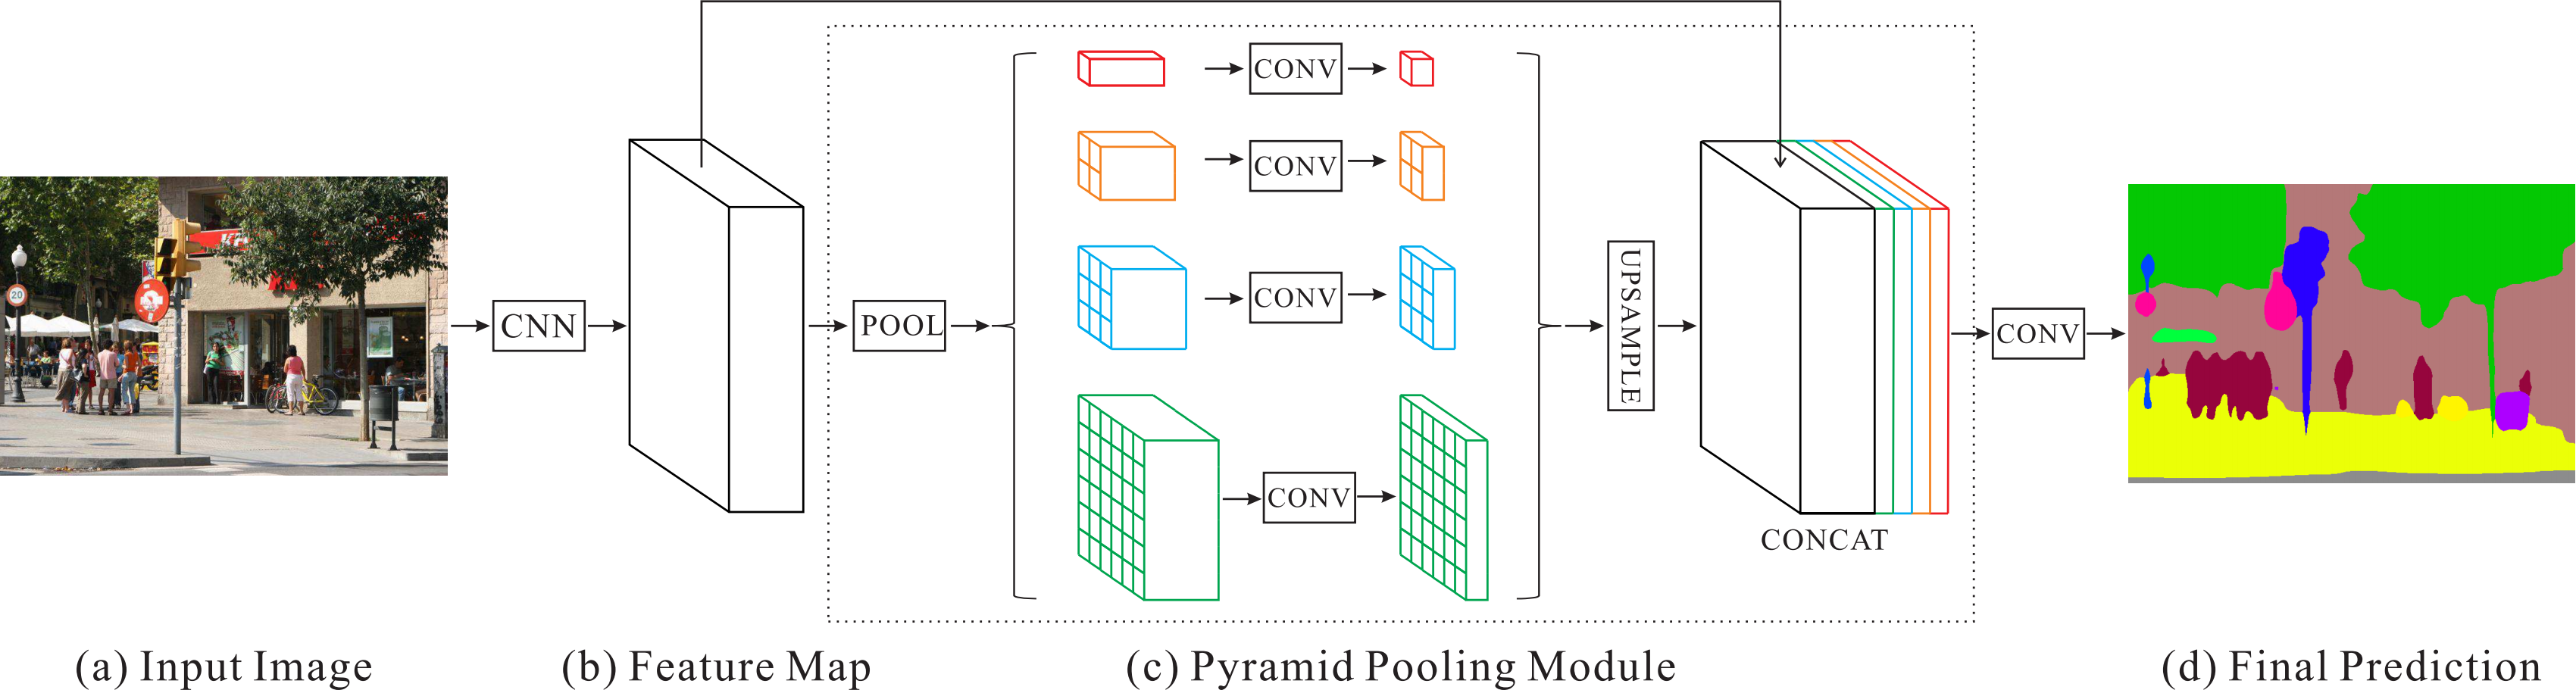
\includegraphics[scale=0.35]{images/PPM.png}
  \caption{
    金字塔池化模型架构\cite{zhao2017PPM}
  }
  \label{fig:PPMfram}
\end{figure}

金字塔池化模型的核心思想是对特征图进行不同尺度的池化操作,然后将池化后的结果拼接(concatenate)起来,以获得多尺度的信息。具体来说,PPM的网络结构如图\ref{fig:PPMfram}所示,通常包括以下几个部分:

(1)多尺度池化:PPM通过对输入的特征图进行不同尺寸的池化操作,例如:1x1、2x2、4x4等。每个尺度的池化结果都有不同的感受野,能够捕捉到图像中不同大小的物体。

(2)上采样:每个池化层得到的特征图通过上采样(upsampling)操作恢复到相同的尺寸,以便可以与其他尺度的池化结果拼接。

(3)拼接(Concatenation):将不同尺度池化后的特征图拼接在一起,生成包含多尺度信息的特征表示。拼接后的特征图具有丰富的全局上下文信息,同时保留了原始特征图的细节信息。

通过对特征图进行多尺度池化操作,金字塔池化模型有效地增强了网络的多尺度上下文信息表达能力,从而提升了图像处理任务的性能。它在很多领域中都有着广泛的应用,特别是在语义分割、目标检测等需要多尺度信息的任务中表现尤为出色,因此我们在本文的变化检测研究中引入了这种模型。
\subsection{平均教师模型}
平均教师模型是Tarvainen等人\cite{Tarvainen2017teacher}于2018年提出的一种半监督学习算法,该算法是针对时间集成模型存在的计算成本大这一缺陷(在每个epoch上更新一次目标标签)提出的改进算法,不同之处是时间集成模型基于时间序列的指数移动平均是在预测结果上,而平均教师模型则是在模型的权重上。在训练步骤上平均模型权重往往会比直接使用最终权重更准确,在训练过程中利用这一点能够训练更优模型。
\begin{figure}[htb]
  \centering
  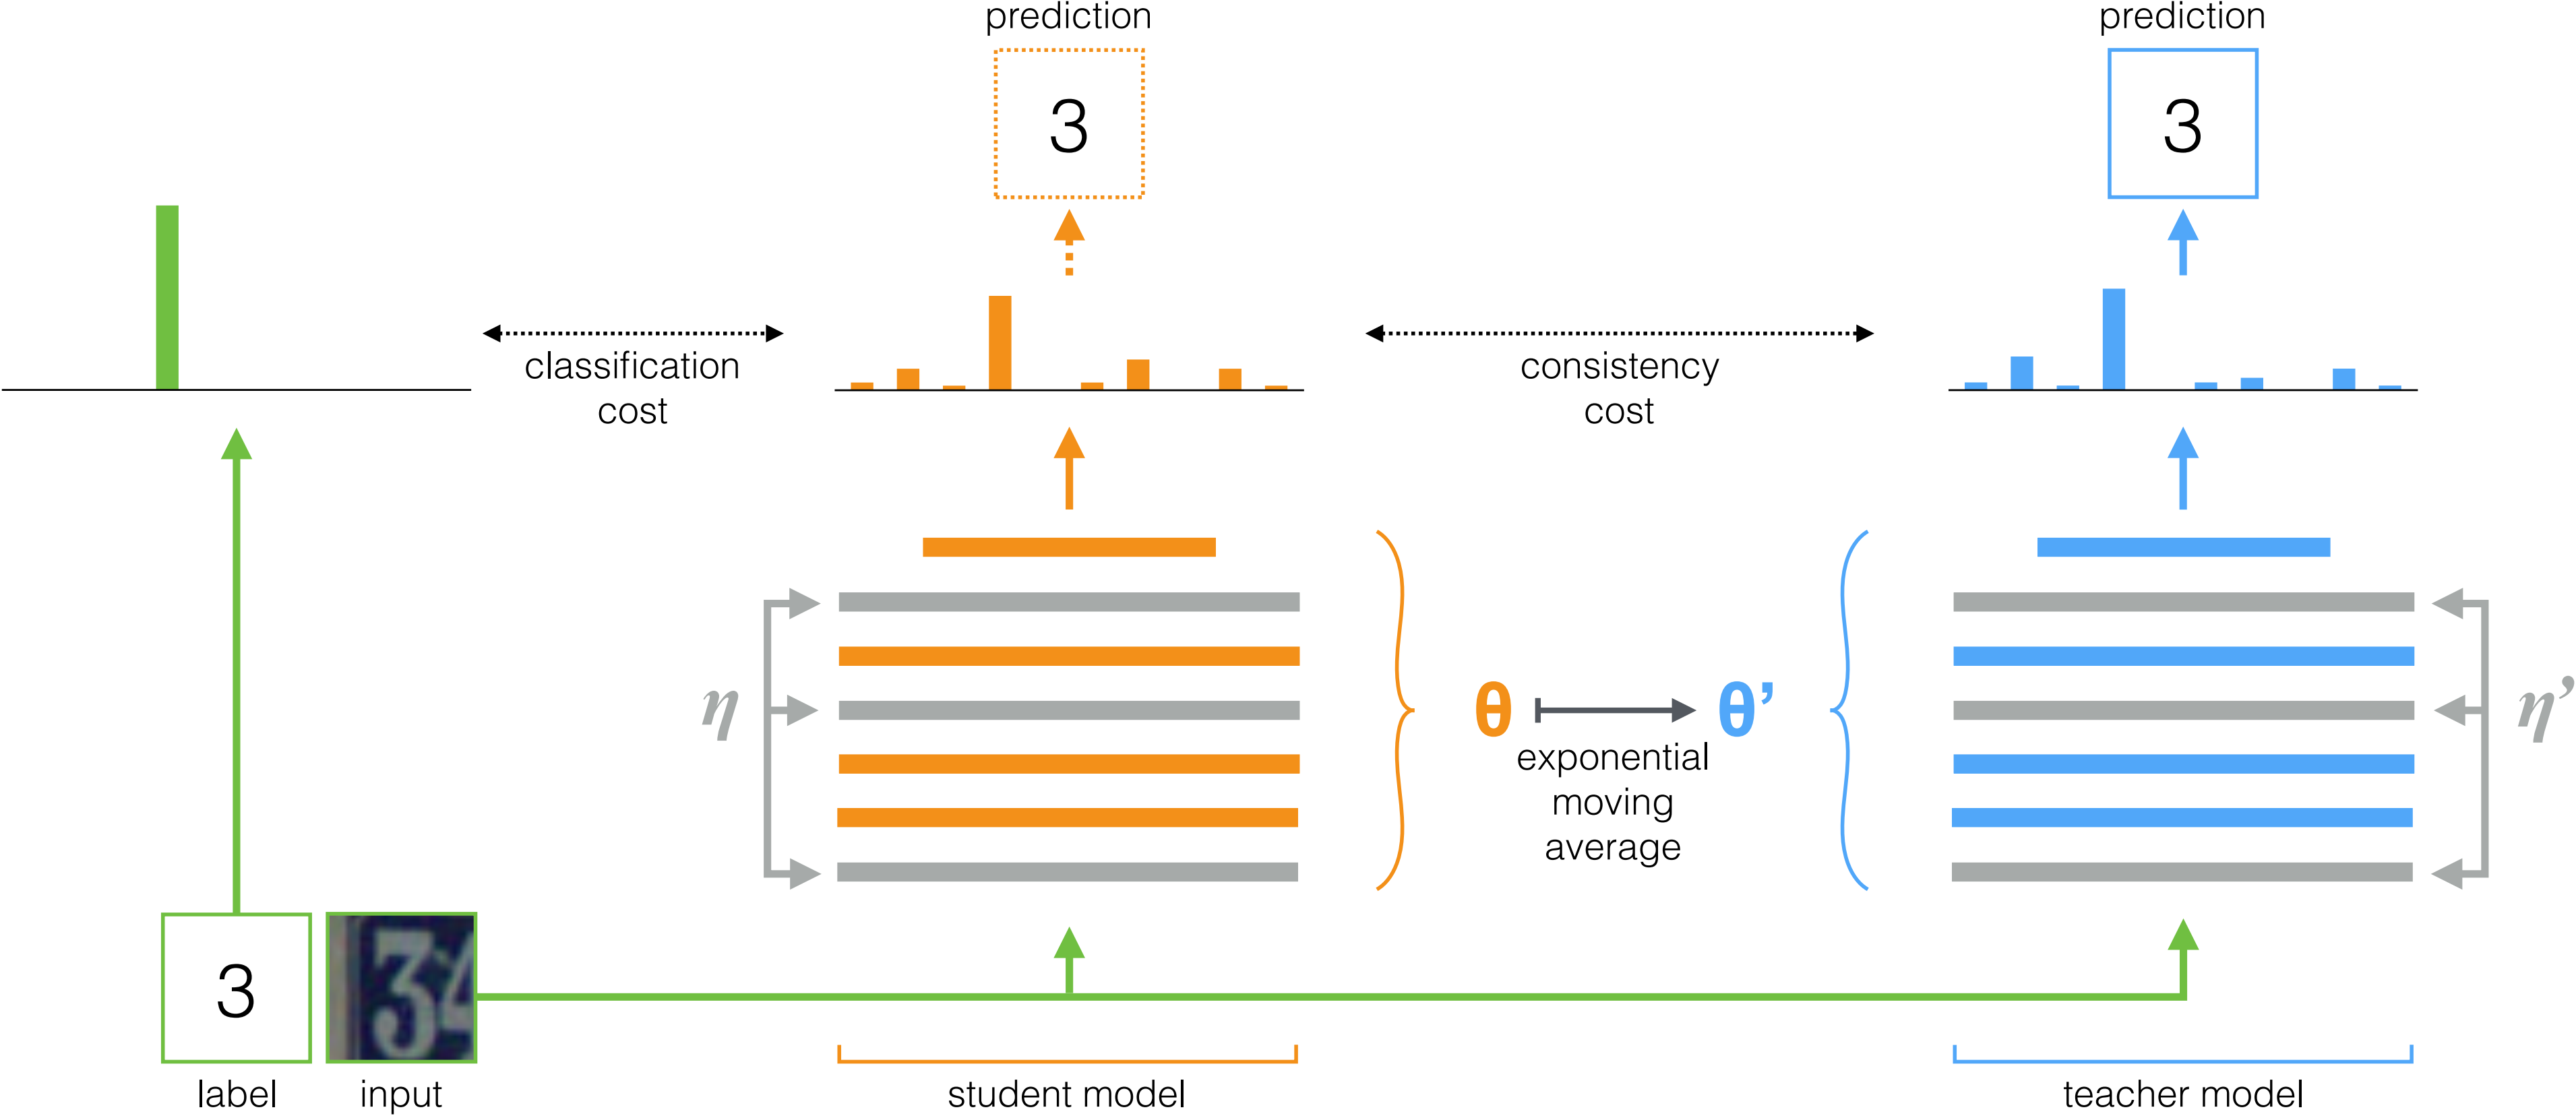
\includegraphics[scale=0.3]{images/mean-teacher.png}
  \caption{
    平均教师模型的网络结构\cite{Tarvainen2017teacher}
  }
  \label{fig:MTfram}
\end{figure}

模型框架如图\ref{fig:MTfram}所示,该半监督框架包含一个教师模型和一个学生模型,由于教师模型的权重是历史学生模型的平均值,故将其称为平均教师模型。核心思想为:使用教师模型用来生成学生模型学习的目标,指导学生模型从无标记样本进行学习,基于一致性正则化原理,认为输入数据添加一个微小的扰动噪声时,模型的预测结果不会发生变化。更正式地说,将一致性成本损失$J$定义为学生模型的预测(模型权重为$\theta$,施加噪声$\eta$)与教师模型的预测(模型权重为$\theta^{\prime}$,施加噪声$\eta^{\prime}$)之间的预期距离,如公式\ref{eq:MTloss}。
\begin{equation}
  \label{eq:MTloss}
  \begin{aligned}
    J(\theta)=\mathbb{E}_{x, \eta^{\prime}, \eta}\left[\left\|f\left(x, \theta^{\prime}, \eta^{\prime}\right)-f(x, \theta, \eta)\right\|^{2}\right]
    \end{aligned}
\end{equation}

$\pi$-模型、时间集成模型和平均教师模型之间的区别在于教师模型预测结果的生成过程。其中$\pi$-模型中教师、学生权重共享,即$\theta^{\prime} = \theta$;时间集成模型通过连续预测的指数移动平均值来估计$f\left(x, \theta^{\prime}, \eta^{\prime}\right)$;在平均教师模型中,将训练步骤t时刻的教师模型权重定义为连续学生模型权重权重的EMA,表示为如下:
\begin{equation}
  \label{eq:MTema}
  \begin{aligned}
    \theta_{t}^{\prime}=\alpha \theta_{t-1}^{\prime}+(1-\alpha) \theta_{t}
    \end{aligned}
\end{equation}

其中$\alpha$为平滑系数超参数。 三种算法之间的另一个区别是,$\pi$-模型直接将训练应用于$\theta^{\prime}$,而时间集成模型和平均教师模型将其视为另一个优化途径。

最终可以在每个训练步骤中随机采样噪声$\eta$和$\eta^{\prime}$,来计算一致性成本$J(\theta)$,并通过随机梯度下降来优化学生模型参数,在此方法中,作者使用均方误差损失作为一致性成本。
% \subsection{Segment Anything Model}
% 自然语言处理领域中基于Transformer的大模型(如GPT和BERT等)展现了跨任务和跨领域的通用性,这进一步推动了视觉领域对通用大模型的需求。受此启发,Meta AI提出了Segment Anything Model\cite{kirillov2023SAM}(SAM),旨在实现对任意图像或视频中的对象进行高效、精准的分割,而无需对具体类别或场景进行额外的训练。其设计理念与通用大模型相似,即通过大规模数据集预训练,使模型具有广泛的泛化能力,能够零样本或少样本适应新任务。其核心思想是通过一个提示驱动(prompt-driven)框架,允许用户通过灵活的提示方式(如点、框、文本描述等)来指定感兴趣的区域,从而实现高度交互性和可控性。SAM的提出不仅是计算机视觉技术发展的延续,更标志着分割任务从任务特定模型向通用模型转变的关键一步,开启了视觉任务中的“分割一切”。
% \begin{figure}[htb]
%   \centering
%   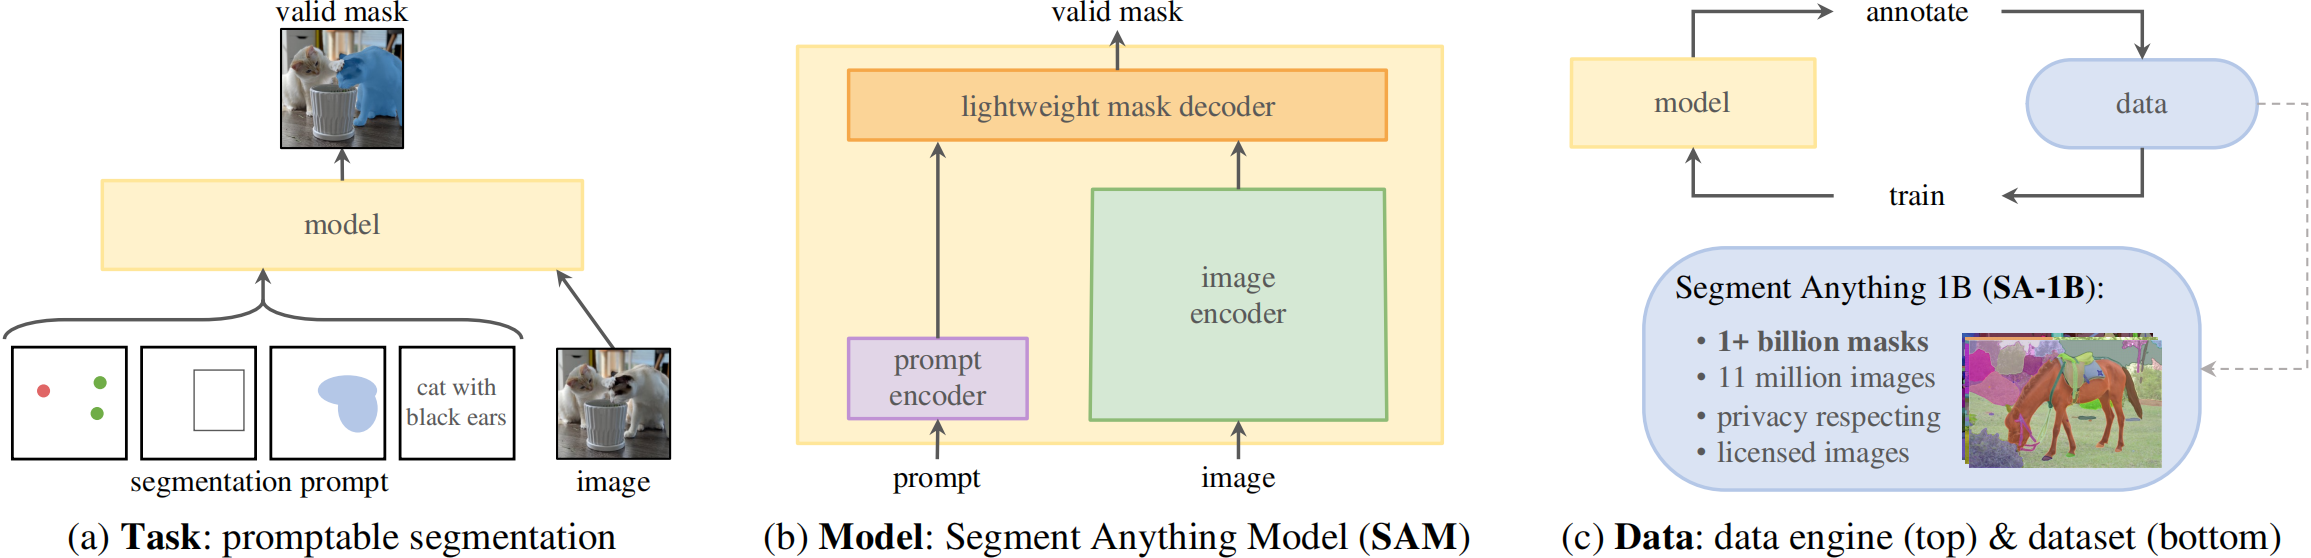
\includegraphics[scale=0.5]{images/SAM1.png}
%   \caption{
%     分割一切基础模型架构\cite{kirillov2023SAM}。
%   }
%   \label{fig:SAMfram}
% \end{figure}

% 为了实现这一目标,SAM引入了三个相互关联的组件来构建了分割的基础模型:一个基于提示的分割任务、一个通过数据标注提供动力并能够通过提示工程实现一系列任务零样本迁移的分割模型(SAM),以及一个用于收集数据集SA-1B的数据引擎,如图\ref{fig:SAMfram}。
% SAM的显著特性是支持多种类型的用户输入作为提示,包括:(1)单点提示,通过在目标对象上指定一个点,SAM能够快速分割该点所属的对象;(2)多点提示,当用户提供多个点时,模型能够根据点之间的关系生成更精确的分割;(3)框提示,通过提供一个边界框,模型可以分割框内的目标对象;(4)文本提示,与自然语言描述结合,通过文本指定需要分割的对象类别。这种灵活的提示驱动机制使SAM在复杂场景下能够通过用户少量交互即可实现高效分割。SAM的网络架构主要由三个主要部分组成,分别是图像编码器(Image Encoder),提示编码器(Prompt Encoder)以及掩码解码器(Mask Decoder)。其中图像编码器就是基于前文介绍的强大的ViT模型,用于提取高质量的全局图像特征,图像编码器在输入时对整幅图像进行一次性编码,生成具有全局上下文的多尺度特征嵌入。提示编码器用于编码用户提供的提示信息,包括点、框或文本等。点或框提示会被转换为位置嵌入,而文本提示则通过专门的文本编码器进行嵌入,提示编码器的设计使模型能够灵活适应多种提示形式。掩码解码器负责将图像编码器生成的全局特征与提示编码器的提示信息融合,生成与提示相关的分割掩码,如图\ref{fig:SAMfram}中所示的过程。此外SAM的强大性能得益于在一个规模空前的大型分割数据集上进行的预训练。该数据集包含超过11亿个图像-分割掩码对,覆盖了广泛的对象类别、场景和视觉条件。通过大规模预训练,SAM获得了卓越的通用性和泛化能力,能够分割未见过的对象或复杂场景中的目标,而无需进一步微调或额外标注。
% \begin{figure}[htb]
%   \centering
%   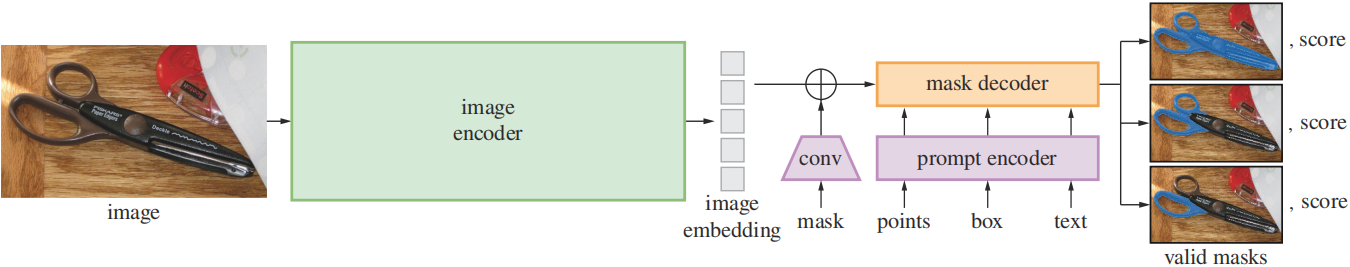
\includegraphics[scale=0.9]{images/SAM.png}
%   \caption{
%     Vision Transformer网络框架\cite{kirillov2023SAM}。
%   }
%   \label{fig:ViTfram}
% \end{figure}

% SAM是一项具有里程碑意义的技术,它通过灵活的提示驱动机制和大规模预训练,构建了一个适用于广泛视觉场景的分割模型。其强大的零样本推理能力和边界预测能力使得其可以不用微调直接用于其他场景和任务,并提供先验知识和辅助推理来优化性能,因此本文的研究工作中引入了SAM模型。
\section{经典半监督变化检测算法}
\subsection{SemiCDNet}
Peng等人\cite{peng2021SemiCDNet}提出了SemiCDNet这种基于生成对抗网络(GAN)的半监督卷积网络。首先,将标记数据和未标记数据输入分割网络,生成初始预测和熵图。然后,为了充分利用未标记数据的潜力,采用两种鉴别器来加强标记数据与未标记数据之间的分割图和熵图的特征分布一致性。在对抗训练过程中,利用未标记信息不断地对生成器进行正则化,从而提高生成器的泛化能力。SemiCDNet是RCR之前唯一可获得的开源SOTA方法,在本文的研究中作为对比方法之一,因此在本小节对其进行简要阐述。

(1)网络框架

SemiCDNet的网络框架如图\ref{fig:SemiCDNetfram}所示,主要包括一个生成器$G$和两个判别器$D_s$和$D_e$,分别用于对齐生成器在无标记数据上的预测概率分布和熵图。
\begin{figure}[htb]
  \centering
  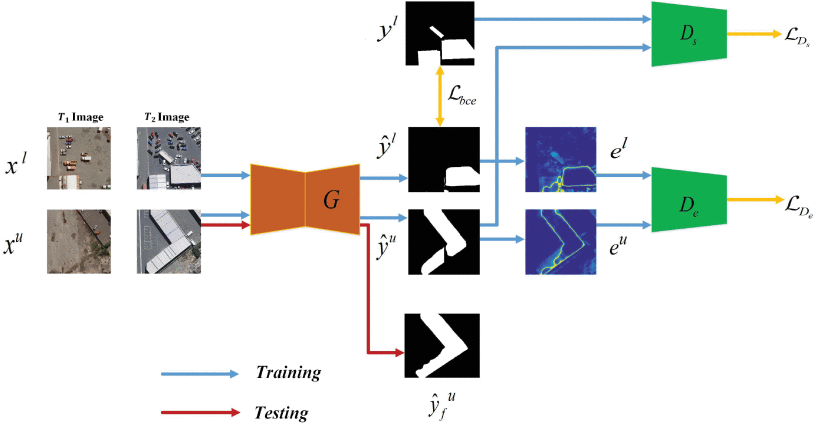
\includegraphics[scale=0.45]{images/SemiCDNetframe.png}
  \caption{
    SemiCDNet网络框架\cite{peng2021SemiCDNet}
  }
  \label{fig:SemiCDNetfram}
\end{figure}

(2)损失函数

主要通过三种损失来训练生成器网络和鉴别器网络,即在标记数据上的加权二值交叉熵损失以及在无标记数据上的分割对抗损失和熵对抗损失。

\textbf{加权二值交叉熵损失}:
为了克服变化检测中变化像素和不变像素之间的样本偏差问题,采用简单的加权二值交叉熵损失。这是一种标准的监督的像素级的分割损失,仅在标记数据上计算这种损失。计算方式可以表示为:
\begin{equation}
  \label{eq:SemiCDNetLossce}
  \begin{aligned}
    \mathcal{L}_{\text {bce }}=-\frac{1}{M}\left[\beta \sum_{j \in y_{+}^{\prime}} \log ( \right. & \left.P\left(y_{j}=1\right)\right)
    & \left.+(1-\beta) \sum_{j \in y_{-}^{l}} \log \left(P\left(y_{j}=0\right)\right)\right]
    \end{aligned}
\end{equation}

其中$\beta$和$1 - \beta$分别表示标记图像的真实标签变化和不变的像素数,$P\left(\cdot\right)$是生成器在像素$j$上的预测输出。

\textbf{分割对抗损失}:
$D_s$用于判断分割图是来自生成器在无标记样本上的预测,还是来自有标注的真实标签,促使生成器$G$在无标记样本的预测$G(x^u)$的特征分布与有标注样本的真实标签$y^l$的特征分布对齐。分割对抗损失计算公式如下:
\begin{equation}
  \label{eq:SemiCDNetLossDs}
  \begin{aligned}
    \mathcal{L}_{D_{s}}=\frac{1}{M} \sum_{x^{l}, y^{l} \in \mathcal{D}_{\mathcal{L}}} \mathcal{L}_{D}\left(y^{l}\right. & \left.\oplus x^{l}, 1\right) \\
    & +\frac{1}{N} \sum_{x^{u} \in \mathcal{D}_{\mathcal{U}}} \mathcal{L}_{D}\left(G\left(x^{u}\right) \oplus x^{u}, 0\right)
    \end{aligned}
\end{equation}

其中$\oplus$表示堆叠拼接操作,$\mathcal{L}_{D}$表示二元交叉熵损失函数,其目的是最小化预测$G(x^u)$与真实$y^l$分布之间的差异。

此外,为了与鉴别器对抗,使用以下对抗损失对分割网络进行优化:
\begin{equation}
  \label{eq:SemiCDNetLossDsadv}
  \mathcal{L}_{\mathrm{adv}}^{D_{s}}=\frac{1}{N} \sum_{x^{u} \in \mathcal{D}_{\mathcal{U}}} \mathcal{L}_{D}\left(G\left(x^{u}\right) \oplus x^{u}, 1\right)
\end{equation}

\textbf{熵对抗损失}:
通常生成器倾向于对标记数据进行低熵、高确定性的预测,而对未标记数据进行的预测具有高熵、低确定性。因此可以对无标记数据进行低熵值的约束。其中熵图(Entropy map)被定义为:
\begin{equation}
  \label{eq:SemiCDNetEntropy}
  E(x)=G(x) \bullet \log [G(x)]
\end{equation}

其中$\bullet$表示点积的操作。$D_s$被训练用于判断熵图是来自有标记数据还是无标记样本上的预测,通过对齐$E(x^u)$和$E(x^l)$之间的特征分布,还可以抑制无标记数据熵图的高不确定性。因此判别器的熵对抗损失通过以下公式计算:
\begin{equation}
  \label{eq:SemiCDNetLossDe}
  \begin{array}{l}
    \mathcal{L}_{D_{e}}=\frac{1}{M} \sum_{x^{l}, y^{\prime} \in \mathcal{D}_{\mathcal{L}}} \mathcal{L}_{D}\left(E\left(x^{l}\right) \oplus x^{l}, 1\right) \\
    +\frac{1}{N} \sum_{x^{u} \in \mathcal{D}_{\mathcal{u}}} \mathcal{L}_{D}\left(E\left(x^{u}\right) \oplus x^{u}, 0\right)
    \end{array}
\end{equation}

生成器的熵对抗损失为:
\begin{equation}
  \label{eq:SemiCDNetLossDeadv}
  \mathcal{L}_{\mathrm{adv}}^{D_{e}}=\frac{1}{N} \sum_{x^{u} \in \mathcal{D}_{\mathcal{u}}} \mathcal{L}_{D}\left(E\left(x^{u}\right) \oplus x^{u}, 1\right)
\end{equation}

于是,SemiCDNet的总体损失为:
\begin{equation}
  \label{eq:SemiCDNetLosstotal}
  \mathcal{L}_{G}=\mathcal{L}_{\text {bce }}+\lambda_{s} \mathcal{L}_{\text {adv }}^{D_{s}}+\lambda_{e} \mathcal{L}_{\mathrm{adv}}^{D_{e}}
\end{equation}
其中$\lambda_{s}$和$\lambda_{e}$分别表示分割对抗损失和熵对抗损失的自定义权重。
\subsection{RCR}
RCR(Revisiting Consistency Regularization)是由Bandara等人\cite{bandara2022RCR}提出的,它们基于聚类假设构建了一个更加广阔的特征扰动空间,这种特征扰动一致性正则化使得模型具有更加强大的泛化能力。本文的研究工作的代码是基于RCR的变化检测网络和训练框架以及前文提到的平均教师模型改进实现的,因而有必要在本小节详细介绍RCR方法。

(1)网络框架

总体框架如图\ref{fig:RCRfram}所示,主要包括三个模块:
1)编码器,用于提取前时相图像和后时相图像的隐藏特征表示;
2)特征差分模块,用于获取变化前和变化后图像的隐藏特征表示Fd的差异;
3)解码器,从隐藏的差异特征表示预测变化掩膜。
\begin{figure}[htb]
  \centering
  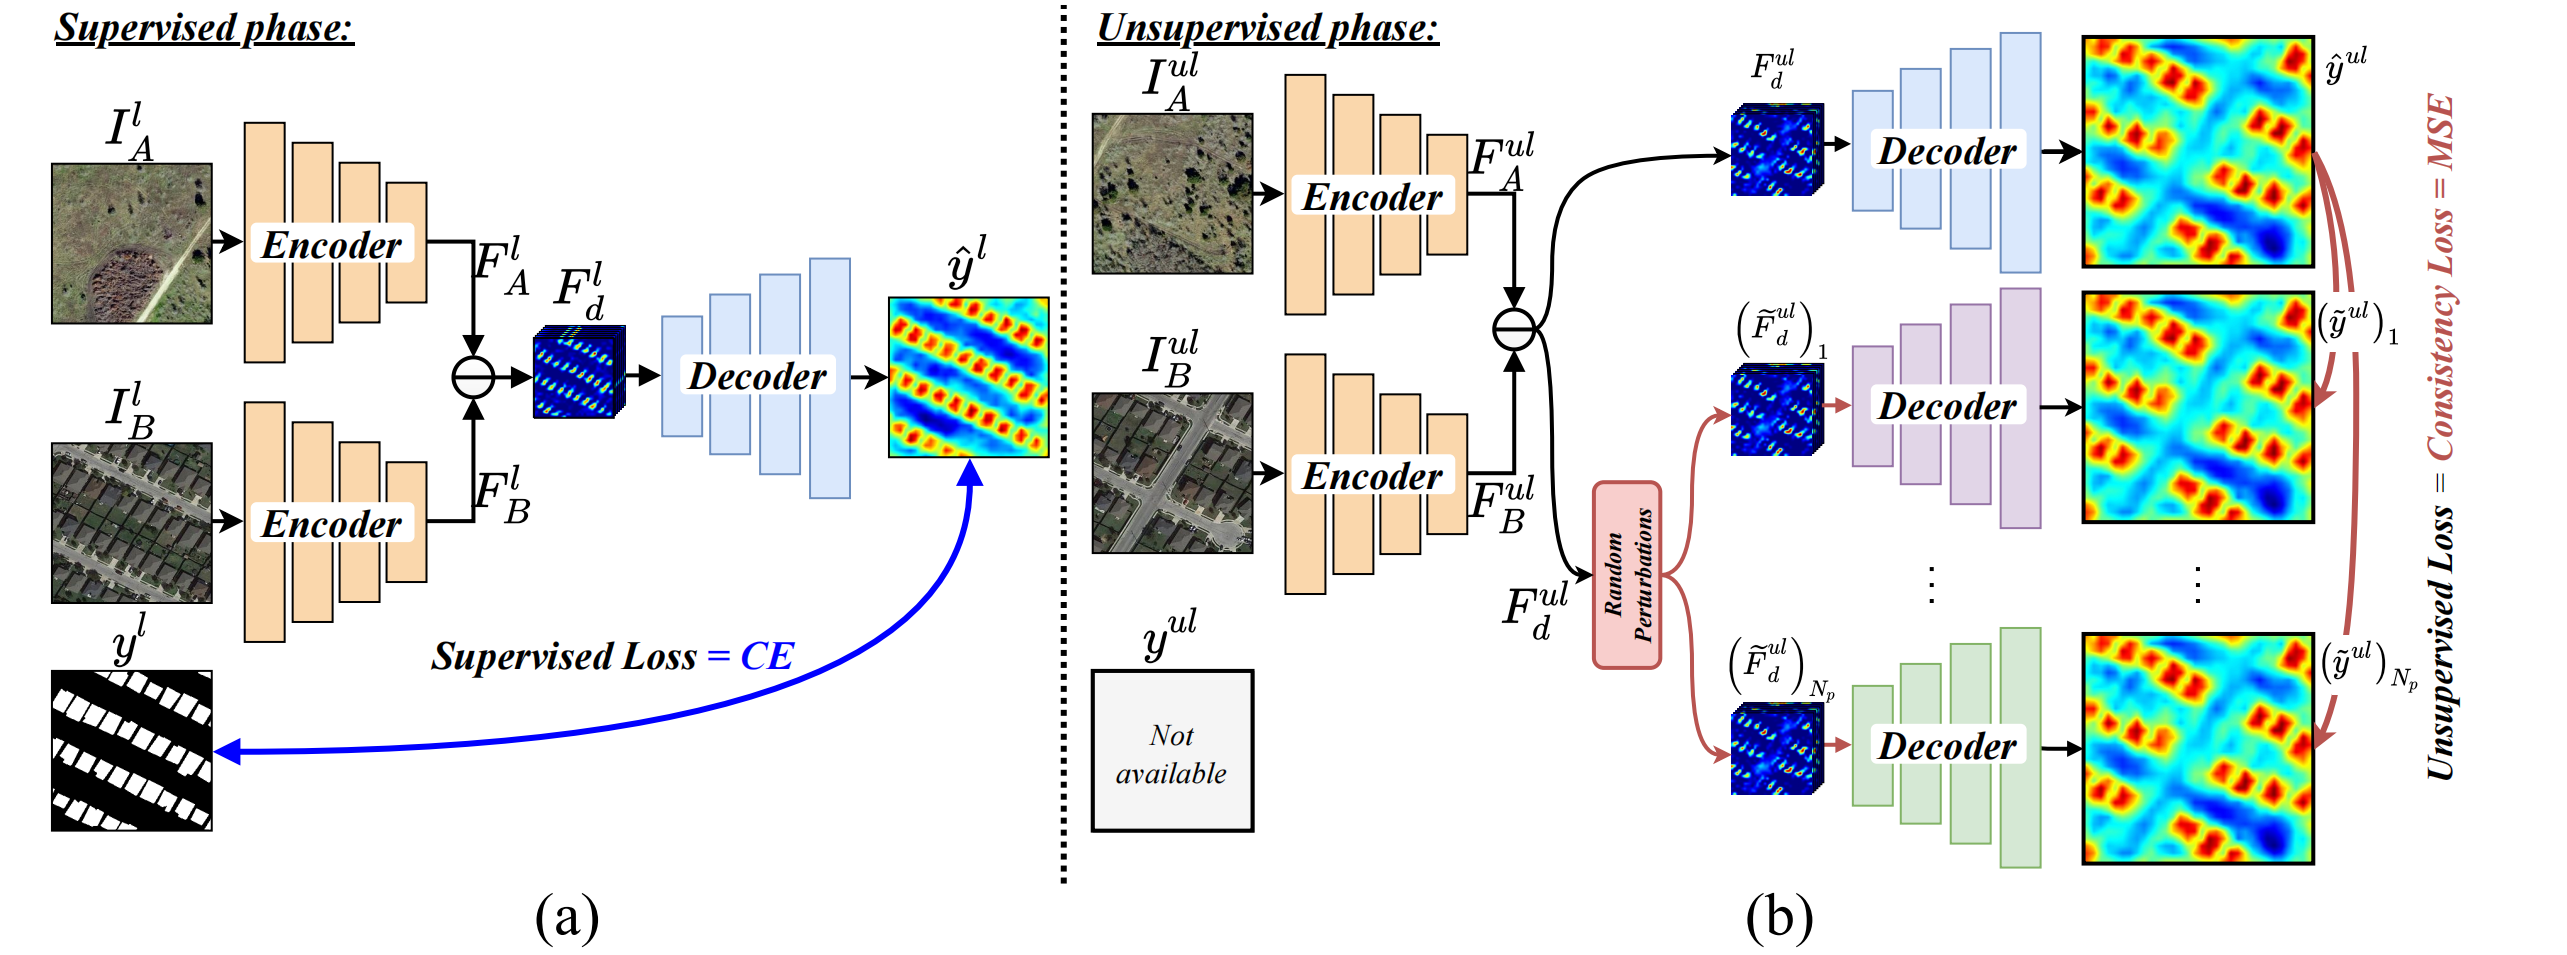
\includegraphics[scale=0.45]{images/RCRframe.png}
  \caption{
    RCR网络框架\cite{bandara2022RCR}
  }
  \label{fig:RCRfram}
\end{figure}

\textbf{编码器$f_{e}$}。对于编码器,RCR使用预训练的ResNet50\cite{He2015ResNet}。编码器的输出是2048维的特征矩阵,空间分辨率为$\frac{H}{4} \times \frac{W}{4}$,其中H和W分别为输入双时相图像$\left \{ I_A, I_B \right \} $的高度和宽度。在孪生网络架构中使用共享权重的双分支编码器,以分别提取两幅图像的隐藏特征表示$F_A$和$F_B$,数学公式表示为:
\begin{equation}
  \label{eq:RCRencode}
  \begin{array}{l}
  F_{A}=f_{e}\left(I_{A}\right), \\
  F_{B}=f_{e}\left(I_{B}\right)
  \end{array}
\end{equation}

\textbf{特征差分模块}。一旦从编码器获得给定双时相图像$\left \{ I_A, I_B \right \} $的隐藏特征表示$F_A$和$F_B$,RCR通过简单地计算$F_A$和$F_B$之间的绝对差值以获得隐藏特征的差分表示$F_d$,随后通过特征金字塔池化模块(Pyramid Pooling Module,PPM)\cite{zhao2017PPM} $f_{PPM}$对其进行处理,以有效地获取不同尺度的变化。用数学方法将特征差分模块内部的过程表示为:
\begin{equation}
  \label{eq:RCRppm}
  F_{d}=f_{\mathrm{PPM}}\left(\left|F_{A}-F_{B}\right|_{1}\right)
\end{equation}

\textbf{编码器$f_{d}$}。解码器的目的是从隐藏的差分特征$F_d$中估计输出的变化概率图$\hat{y} $。j解码器中通过一系列亚像素卷积上采样模块\cite{shi2016upsample},直到特征达到输入双时图像的空间分辨率$H \times w$。解码器内部的过程可以用数学表达为:
\begin{equation}
  \label{eq:RCRdecode}
  \hat{y}=f_{d}\left(F_{d}\right)
\end{equation}

(2)训练管道

训练以上变化检测的过程包含两个部分,一部分是在少量标注样本上进行的监督训练,另一部分则是在大量无标注样本上进行的无监督训练。

\textbf{监督训练}。
在这一阶段,RCR只预测标记训练数据所隐含的兴趣变化:$\mathcal{D}_{l}=\left\{\left\{I_{A, i}^{l}, I_{B, i}^{l}\right\}, y_{i}^{l}\right\}_{i=1}^{N_{l}}$, 其中$\left\{I_{A, i}^{l}, I_{B, i}^{l}\right\}$表示第$i$个双时相图像对,$y_{i}^{l}$是相应的真实变化掩码标注,${N_{l}}$是标记数据集的大小。利用预测值与真实标签之间计算的交叉熵(Cross Entropy, CE)损失\cite{murphy2012CE}作为监督损失$L_{sup}$,如公式\ref{eq:RCRLosssup}所示:
\begin{equation}
  \label{eq:RCRLosssup}
  \mathcal{L}_{\text {sup }}=\operatorname{CE}\left(\hat{y}_{i}^{l}, y_{i}^{l}\right)
\end{equation}

整个过程如图\ref{fig:RCRfram}-a所示。

\textbf{无监督训练}。
在这一阶段,除了标记数据$\mathcal{D}_{l}$,我们还使用未标记的双时相图像对$\mathcal{D}_{u}=\left\{I_{A, i}^{ul}, I_{B, i}^{ul}\right\}_{i=1}^{N_{ul}}$,其中$\left\{I_{A, i}^{ul}, I_{B, i}^{ul}\right\}$是第i个未标记的双时相图像对,$N_{ul}$是未标记数据集的大小,通常假设它大于标记数据集的大小(即$N_{u l} \gg N_{l}$)。为了有效地利用这些容易获得的未标记双时相图像来提高变化检测模型$f_{C D}(\cdot)$的性能,RCR提出了一个基于未标记数据的无监督损失$L_{unsup}$,它提供了一个额外的训练信号来优化$f_{C D}(\cdot)$的参数。所提出的无监督损失基于半监督学习中的聚类假设,其中RCR强制$f_{C D}(\cdot)$的预测在深度特征差分图$F_d$上施加不同随机扰动下依然保持一致,如图\ref{fig:RCRfram}-b所示。

定义$\left\{\left(\widetilde{F}_{d, i}^{u l}\right)_{1}, \cdots,\left(\widetilde{F}_{d, i}^{u l}\right)_{p}, \cdots,\left(\widetilde{F}_{d, i}^{u l}\right)_{p=N_{p}}\right\}$作为第i个未标记双时相图像对$\left\{I_{A, i}^{ul}, I_{B, i}^{ul}\right\}$的隐藏差分特征$F_{d, i}^{u l}$的随机扰动版本集合。接下来,RCR通过主解码器$f_d(\cdot)$对$F_{d, i}^{u l}$进行处理,得到预测的变化概率图为:
\begin{equation}
  \label{eq:RCRpredict}
  \hat{y}_{i}^{u l}=f_{d}\left(F_{d, i}^{u l}\right)
\end{equation}

以及通过一组与$f_d(\cdot)$设计相似的辅助解码器处理隐藏特征差分图的每个扰动版本,得到它们对应的预测$\left(\widetilde{y}_{i}^{u l}\right)_{p}$为:
\begin{equation}
  \label{eq:RCRauxpredict}
  \left(\widetilde{y}_{i}^{u l}\right)_{p}=f_{d}^{p}\left(\left(\widetilde{F}_{d, i}^{u l}\right)_{p}\right), \text { where } p=1, \ldots, N_{p}
\end{equation}

接下来,RCR通过定义无监督损失$L_{unsup}$来强制$\left\{\left(\widetilde{y}_{i}^{u l}\right)_{p}\right\}_{p=1}^{N_{p}}$与$\hat{y}_{i}^{u l}$一致,如下公式所示:
\begin{equation}
  \label{eq:RCRLossu}
  \mathcal{L}_{\text {unsup }}=\sum_{p=1}^{N_{p}} \mathbf{d}\left(\left(\widetilde{y}_{i}^{u l}\right)_{p}, \hat{y}_{i}^{u l}\right)
\end{equation}

其中$d(\cdot)$是距离度量,用于测量预测之间的不相似性,在RCR中Bandara等人使用均方误差(Mean Squares Error,MSE)作为$d(\cdot)$。

(3)扰动方式

在RCR中,在输入特征上采取的扰动方式有以下几种:

1)随机特征噪声:随机生成一个三维噪声张量,然后根据$F_{d, i}^{u l}$中值的大小对其进行缩放,并将其添加到隐藏特征差分图中,得到一个扰动版本。

2)随机特性丢弃:首先通过阈值从特性差异图中选取出10$\%$到40$\%$的最需要的区域,生成掩膜,然后沿着通道维度,将潜在差分特征和该掩膜进行逐像素相乘,从而丢弃掉那些不需要的区域特征。

3)引导特征剪切:我们基于预测的变化图,从差分特征图中随机取零,得到扰动特征图。

4)内容和对象覆盖:基于变化检测网络的输出对变化类或不变类保持不变的假设,通过变化掩码掩盖隐藏差分特征图中的变化区域,或者通过不变掩膜掩盖隐藏差分特征图中的不变区域,创建隐藏差分特征图的两个扰动版本。

5)特征VAT\cite{2019VAT}:在变化最大的方向上对差分特征图应用对抗性扰动。
\subsection{FPA}
FPA(Feature-Prediction Alignment)是张等人\cite{Zhang2023FPA}2023年提出的半监督变化检测框架。FPA提出了两种对齐策略,来有效地利用未标记的双时相图像对进行训练。首先,设计了一种类感知特征对齐(Feature Alignment,FA)策略,将从不同未标记图像对(即跨区域)中提取的区域级变化/无变化特征进行对齐,以减少同一类内的特征差异。其次,设计了一种像素级预测对齐(Pixel- wise Prediction Alignment, PA)方法,将强增强未标记图像对的像素级变化预测与弱增强对应的伪标签进行对齐,以降低各种具有物理意义的图像对变换的预测不确定性。其总体框架如图\ref{fig:FPAfram}所示。其中使用的变化检测网络和监督训练过程都和RCR\cite{bandara2022RCR}相同,因此以下内容主要介绍其新颖的无监督训练部分。
\begin{figure}[htb]
  \centering
  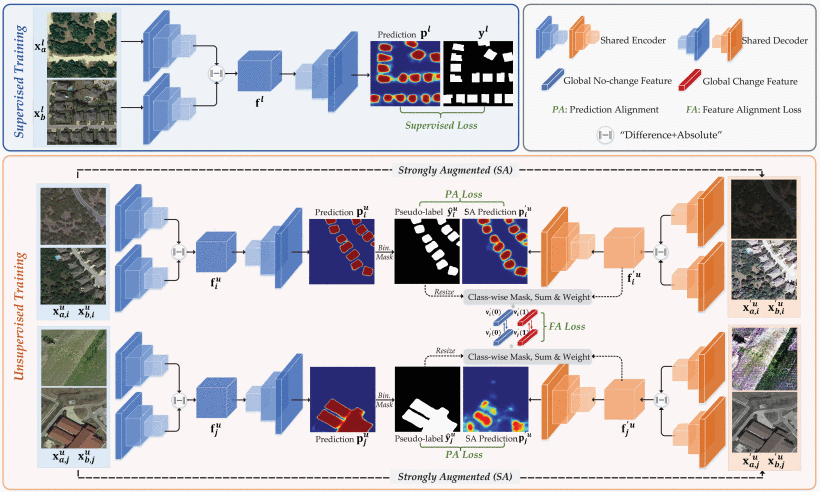
\includegraphics[scale=0.55]{images/FPAframe.png}
  \caption{
    FPA网络框架\cite{Zhang2023FPA}
  }
  \label{fig:FPAfram}
\end{figure}

(1)类感知特征对齐

类感知特征对齐目的是在训练阶段实现小批量内不同未标记图像对的类内全局特征对齐。具体说来,首先对原始的无标记图像对施加弱增强操作,得到一个弱增强无标记图像对$\left\{\mathbf{x}_{a}^{u}, \mathbf{x}_{b}{ }^{u}\right\}$,并进一步继续对其施加强增强操作得到其对应的强增强图像对$\left\{\mathbf{x'}_{a}^{u}, \mathbf{x'}_{b}{ }^{u}\right\}$:
\begin{equation}
  \label{eq:FPAaug}
  \begin{aligned}
    \mathbf{x}_{a}^{\prime}{ }^{u} & =\operatorname{RandAugment}\left(\mathbf{x}_{a}{ }^{u}\right), \\
    \mathbf{x}_{b}^{\prime}{ }^{u} & =\operatorname{RandAugment}\left(\mathbf{x}_{b}{ }^{u}\right)
  \end{aligned}
\end{equation}

其中$RandAugment(\cdot)$表示从预定义的增强列表中随机抽样两个连接的强增强操作,增强列表如图\ref{fig:FPAstrongAug}所示,包括Identity,Contrast,Autocontrast,Brightness,,Color,,Equalize,Sharpness,Posterize和Solarize等9种常用增强方式,其中a-g分别是(a)原始图像;(b)Identity;(c)Contrast;(d)Autocontrast;(e)Brightness;(f)Color;(g)Equalize;(h)Sharpness;(i)Posterize;(j)Solarize。
\begin{figure}[htb]
  \centering
  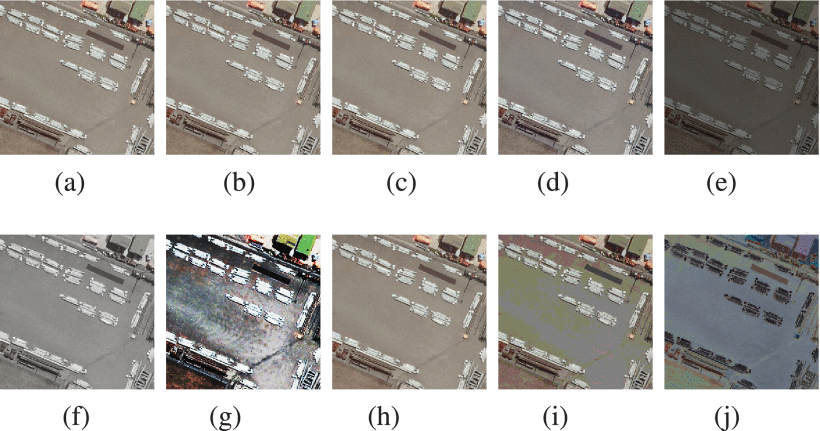
\includegraphics[scale=0.55]{images/Strong_aug.png}
  \caption{
    FPA使用的强增强操作列表\cite{Zhang2023FPA}
  }
  \label{fig:FPAstrongAug}
\end{figure}

然后,通过编码器分别从$\left\{\mathbf{x}_{a}^{u}, \mathbf{x}_{b}^{u}\right\}$和$\left\{\mathbf{x'}_{a}^{u}, \mathbf{x'}_{b}{ }^{u}\right\}$中提取特征映射$f^u$和强增强特征映射$f'^u$。为了模型训练的鲁棒性,以解码器从$f^u$中提取的弱增强预测映射$p^u$作为伪标签参考,指导在强增强特征图$f'^u$上进行特征对齐操作。为了实现这一步,通过固定阈值筛选掉$p^u$中部分含噪较高的像素预测值:
\begin{equation}
  \label{eq:FPAthresh}
  \mathbf{m}^{u f}(i, j, k)=\left\{\begin{array}{ll}
    1, & \text { if } \quad \mathbf{p}^{u}(i, j, k)>\tau \\
    0, & \text { else }
    \end{array}\right.
\end{equation}

接下来对$m^{u f}$进行最近邻下采样为$\mathbf{m}^{u f} \in \mathbb{R}^{H / s \times W / s \times 2}$以适应强增强特征图$f'^u$的空间分辨率。如此一来便可以基于预测掩码$m^{u f}$和强增强特征映射$f'^u$,提取出分类全局特征向量,记为$\mathbf{v}^{\prime} \in \mathbb{R}^{2 \times C}$,以上过程用公司可表示为如下:
\begin{equation}
  \label{eq:FPAmetafeat}
  \mathbf{v}^{\prime}(k)=\frac{1}{\boldsymbol{w}(k)} * \sum_{i=1}^{H / s} \sum_{j=1}^{W / s} \mathbf{f}^{u}(i, j) * \mathbf{m}^{u f}(i, j, k)
\end{equation}

其中$*$表示逐像素点积运算,$\boldsymbol{w}(k)$为类权像素和,即变化类别的像素总数,计算过程如\ref{eq:FPAsum},$\epsilon = 1e-8$是一个很小的余量,以避免每个类的权重可能为零。
\begin{equation}
  \label{eq:FPAsum}
\boldsymbol{w}(k)=\sum_{i=1}^{H / s} \sum_{j=1}^{W / s} \mathbf{m}^{u f}(i, j, k)+\epsilon
\end{equation}

最后为了实现跨区域的类内特征对齐,FPA通过增加它们的余弦相似度约束来使一个小批中的所有分类全局特征向量彼此对齐,无监督特征对齐损失计算如下:
\begin{equation}
  \label{eq:FPALossf}
  \begin{aligned}
    \mathcal{L}_{u}^{F A}= & \frac{1}{2 B B} \sum_{k=1}^{2} \sum_{i=1}^{B} \sum_{j=1}^{B} \mathbb{I}\left(\boldsymbol{w}_{i}(k)>0, \boldsymbol{w}_{j}(k)>0\right) \\
    & \cdot \frac{1}{2}\left(1-\frac{\mathbf{v}_{i}^{\prime}(k) * \mathbf{v}_{j}^{\prime}(k)}{\left\|\mathbf{v}_{i}^{\prime}(k)\right\|\left\|\mathbf{v}_{j}^{\prime}(k)\right\|+\epsilon}\right)
    \end{aligned}
\end{equation}

其中,$\mathbf{v}_{i}^{\prime}(k)$和$\mathbf{v}_{j}^{\prime}(k)$分别表示当前小批量(B为小批量大小)中第i和第j个未标记图像对的第k类全局特征向量。$\left(\mathbf{v}_{i}^{\prime}(k) * \mathbf{v}_{j}^{\prime}(k) /\left\|\mathbf{v}_{i}^{\prime}(k)\right\|\left\|\mathbf{v}_{j}^{\prime}(k)\right\|\right)$表示$\mathbf{v}_{i}^{\prime}(k)$与$\mathbf{v}_{j}^{\prime}(k)$之间第k类全局特征的余弦相似度,其本身取值范围为[−1,1],为了便于训练FPA将其重映射到了[0,1]。

(2)像素级预测对齐

像素级预测对齐的目的是使强增强图像对的输出与弱增强图像对的输出保持一致,从而使模型获得鲁棒的特征提取能力。为此,FPA中引入了\cite{sohn2020fixmatch}的置信度一致性学习策略,从半监督图像分类任务适用到SSCD的像素级任务。对于从弱增强图像对获取到的像素级的变化概率图$\mathbf{p}^{u}$,按以下方式生成伪标签映射$\hat{\mathbf{y}}^{u} \in \mathbb{R}^{H \times W}$:
\begin{equation}
  \label{eq:FPApesudo}
  \hat{\mathbf{y}}^{u}(i, j)=\underset{k=\{0,1\}}{\arg \max } \mathbf{p}^{u}(i, j, k)
\end{equation}

同样,为了减少噪声伪标签的干扰,对从$\mathbf{p}^{u}$生成的基于置信度的变化掩码$\mathbf{m}^{u p}\in \mathbb{R}^{H \times W}$基于一个固定阈值仅筛选出那些最为可信的预测像素。
\begin{equation}
  \label{eq:FPAfilter}
  \mathbf{m}^{u p}(i, j)=\left\{\begin{array}{ll}
    1, & \text { if } \quad \mathbf{p}^{u}\left(i, j, \hat{\mathbf{y}}^{u}(i, j)\right)>\tau \\
    0, & \text { else. }
    \end{array}\right.
\end{equation}

其中$\tau$是固定阈值的取值,在FPA中默认设置为0.95。

因此,第k个图像对的像素级预测对齐损失,可以表示为公式\ref{eq:FPALossp}和公式\ref{eq:FPALosspavg}:
\begin{equation}
  \label{eq:FPALossp}
  \mathcal{L}_{u}^{P A}(k)=\frac{1}{H W} \sum_{i=1}^{H} \sum_{j=1}^{W} \operatorname{CE}\left(\mathbf{p}^{\prime u}(i, j), \hat{\mathbf{y}}^{u}(i, j)\right) * \mathbf{m}^{u p}(i, j),
\end{equation}
\begin{equation}
  \label{eq:FPALosspavg}
  \mathcal{L}_{u}^{P A}=\frac{1}{B} \sum_{k=1}^{B} \mathcal{L}_{u}^{P A}(k)
\end{equation}

最终整个无监督训练的损失函数即为类感知特征对齐损失和像素级预测对齐损失的求和:
\begin{equation}
  \label{eq:FPALossu}
  \mathcal{L}_{u}=\mathcal{L}_{u}^{F A}+\mathcal{L}_{u}^{P A}
\end{equation}
\section{实验指标}
为了更好地衡量所有模型的性能,我们引入了2个广泛使用的变化检测评价指标,包括交并比(Intersection over Union,IoU)和总体精确度(Overall Accuracy,OA)。IoU、OA的取值范围均为0-100($\%$)。对于所有这些指标,该值越大,变化检测性能就越好,但是在变化检测任务中,由于二分类和不平衡的类别不平衡,OA总体上都是一个很高的值。它们的计算表述如下:
\begin{equation}
  \label{eq:IoU}
  I o U=\frac{T P}{T P+F P+F N},
\end{equation}
\begin{equation}
  \label{eq:OA}
  O A=\frac{T P+T N}{T P+T N+F N+F P}
\end{equation}

其中$TP$和$TN$分别表示正确识别的变化像素数和未变化像素数。相反,$FP$表示未发生变化的像素被错误地分类为变化的像素的数量,$FN$表示发生变化的像素被错误地识别为未变化的像素的数量。此外,由于我们更关注变化区域的预测性能,并且变化类和背景类极度不平衡,因此在实验中使用变化类别区域的平均交并比 ($IoU^c$)作为评价指标。
\section{实验数据集介绍}
本文中所有方法都在十个基准公开变化检测数据集上进行了实验,分别是LEVIR-CD\cite{chen2020levircd}、LEVIR-CD+\cite{chen2020levircd}、WHU-CD\cite{ji2018whu}、EGY-CD\cite{holail2023EGYCD}、HRCUS-CD\cite{zhang2023HRCUS}、Change Detection Dataset(CDD)\cite{Lebedev2018CDD}、GZ-CD\cite{peng2021SemiCDNet}、DSIFN-CD\cite{zhang2020dsifn}、SYSU-CD\cite{shi2022SYSU}和CL-CD\cite{liu2022CLCD}。其中,这些数据集涵盖了不同的分辨率(0.03m-2.0m)、不同的数据大小(2400至20000对)、不同的标注类别(二值建筑物或多类)、不同的图像对时间跨度(1年-16年),汇总如表\ref{datasets}所示,二值建筑物变化检测数据集部分样例展示如图\ref{fig:building_sample}所示,多类变化检测数据集部分样例展示如图\ref{fig:mutil_sample}所示。
\begin{table*}[!htbp]
  \centering
  \caption{本文所使用的公开数据集}
  \begin{tabular}{c|c|c|c|c|c|c}
  \toprule[1pt]
  % \rowcolor[HTML]{DAE8FC}
  \rowcolor[HTML]{ECF4FF}
  \textbf{变化类别} &
    \textbf{数据集} &
    \textbf{空间分辨率} &
    \textbf{大小} &
    \textbf{样本数量} &
    \textbf{时间跨度} &
    \textbf{链接}
    \\
    % \hline
    \midrule
   & LEVIR-CD  \cite{chen2020levircd}  & 0.5m & 1024 $\times$ 1024   & 637 & 5到14年 &\href{https://justchenhao.github.io/LEVIR/}{\textcolor{blue}{Link}} \\
   \cline{2-7}
   & LEVIR-CD+ \cite{chen2020levircd}  & 0.5m & 1024 $\times$ 1024   & 985  & 5到14年
  &\href{https://justchenhao.github.io/LEVIR/}{\textcolor{blue}{Link}}\\
   \cline{2-7}
    &WHU-CD \cite{ji2018whu}&
    0.2m &
    15354$\times$32507 &
    1 &
    2012年至2016年
  &\href{http://study.rsgis.whu.edu.cn/pages/download/building_dataset.html}{\textcolor{blue}{Link}}\\
  \cline{2-7}
   & GZ-CD \cite{peng2021SemiCDNet}&
    0.55m &
    Varying &
    19 &
    2006年至2019年
  &\href{https://github.com/daifeng2016/Change-Detection-Dataset-for-High-Resolution-Satellite-Imagery}{\textcolor{blue}{Link}}\\
  \cline{2-7}
     & EGY-BCD \cite{holail2023EGYCD}&
    0.25m &
    256 $\times$ 256 &
    6091 &
    2015年至2022年
  &\href{https://github.com/oshholail/EGY-BCD}{\textcolor{blue}{Link}}\\
  \cline{2-7}
  \multirow{-5}{*}{\textbf{\begin{tabular}[c]{@{}c@{}} 建筑物\end{tabular}}} &
  HRCUS-CD \cite{zhang2023HRCUS}&
    0.5m &
    256 $\times$ 256 &
    11388 &
    混合
  &\href{https://github.com/zjd1836/AERNet}{\textcolor{blue}{Link}}\\
    \midrule
    % \hline
   & CDD\cite{Lebedev2018CDD}   & 0.03m-1.0m & 256$\times$256  & 16000    & 混合
   &\href{https://drive.google.com/uc?id=0B-IG2NONFdciOWY5QkQ3OUgwejQ&export=download}{\textcolor{blue}{Link}} \\
   \cline{2-7}
   & DSIFN-CD \cite{zhang2020dsifn} &Unknown & 512$\times$512   & 3940    & 未知
  &\href{https://github.com/GeoZcx/A-deeply-supervised-image-fusion-network-for-change-detection-in-remote-sensing-images/tree/master/dataset}{\textcolor{blue}{Link}} \\
   \cline{2-7}
   & SYSU-CD\cite{shi2022SYSU} &0.5m & 256$\times$256 & 20000  & 2007年至2014年
   &\href{https://github.com/liumency/SYSU-CD}{\textcolor{blue}{Link}} \\
   \cline{2-7}
  \multirow{-4}{*}{\textbf{\begin{tabular}[c]{@{}c@{}} 多类\end{tabular}}}
   & CL-CD \cite{liu2022CLCD} &0.5-2.0m & 512$\times$512 & 600  & 2017年至2019年
   &\href{https://github.com/liumency/CropLand-CD}{\textcolor{blue}{Link}} \\
  \midrule
  \end{tabular}
  \label{datasets}
  \end{table*}

\textbf{LEVIR-CD数据集}:该数据集是一个综合性的遥感建筑变化检测数据集,由637对超高分辨率的谷歌地球图像块组成,每个块的空间分辨率为0.5m,尺寸为$1024\times1024$像素。这些双时相图像来自美国德克萨斯州七个城市的20个不同地点,双时相图像拍摄于2002年至2018年间,时间跨度在5到14年。经过切割之后,该数据集的分布是这样的:训练集占比为70$\%$(7120对),验证集占比为10$\%$(1024对),测试集占另外20$\%$(2048对)。
\begin{figure}[!htb]
  \centering
  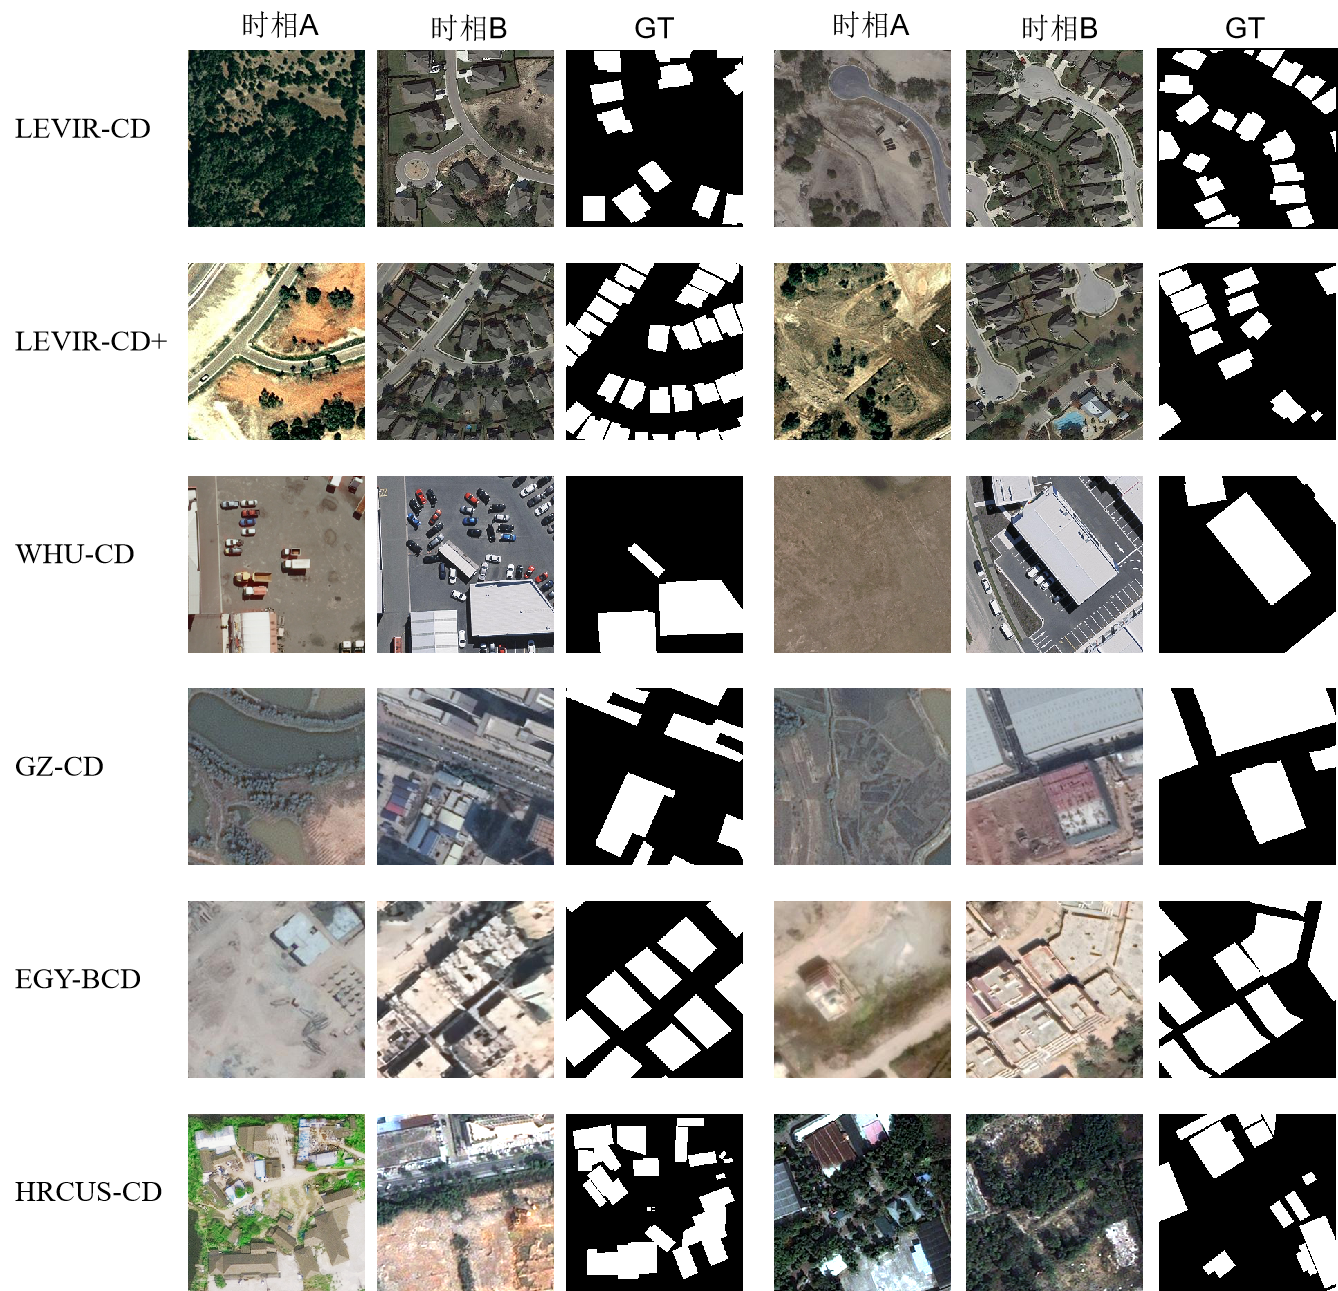
\includegraphics[scale=0.65]{images/building_sample.png}
  \caption{
    建筑物变化检测数据集部分样例图
  }
  \label{fig:building_sample}
\end{figure}

\textbf{LEVIR-CD+数据集}:LEVIR-CD+是对现有LEVIR-CD数据集的一个扩展版本,包含的样本数量扩充到985对$1024\times1024$像素的图像对,其中来自LEVIR-CD的637对用于训练,我们将其中的10$\%$用于验证,其余扩展的385对用于测试。

\textbf{WHU-CD数据集}:原始数据集由单个双时相图像对组成,其中包括2012年和2016年拍摄的新西兰克赖斯特彻奇的两张航拍图像。以同样的切割方式,我们将其分成7434个不重叠的图像对,每个图像对的大小为$256\times256$像素。训练、验证和测试数据集分别由5947、743和744对图像组成。

\textbf{GZ-CD数据集}:GZ-CD数据集的双时相图像收集于2006年至2019年,覆盖中国广州郊区。共收集了19幅不同尺寸的红、绿、蓝波段空间分辨率为0.55m的超分辨率图像,注释集中在建筑物变化上。经过切割成统一尺寸之后,共包含3603对样本,其中训练样本2882对,验证样本360对,测试样本361对。

\textbf{EGY-BCD数据集}:EGY-CD数据集包含6091张2015 - 2022年拍摄的$256 \times 256$像素的图像对,空间分辨率为0.25m/像素,主要标注了埃及4个城市和沿海地区的建筑变化区域。不用额外处理,我们将其中70$\%$用于训练,20$\%$用于验证,剩下的10$\%$用于测试。

\textbf{HRCUS-CD数据集}:该数据集由11388对高分辨率遥感图像组成,裁剪为$256 \times 256$像素,空间分辨率为0.5m。主要分为两个征集区,一个是城市建成区,时间跨度从2019年到2022年,建筑变化面积较少;另一个是正在建设的新城区,从2010年到2018年,包含农田、山地等多种地貌,建筑物变化面积较大。

\textbf{CDD数据集}:CDD数据集包含16000对$256\times256$像素的双时相图像对,像素分辨率从0.03到1米不等。所有这些双时间图像都是从谷歌地球收集的7对$4725\times2700$像素的季节性变化图像对中裁剪出来的。分别有10000对、3000对和3,000对用于训练、验证和测试。

\textbf{DSIFN-CD数据集}:DSIFN-CD是在谷歌地球上人工采集的,它由覆盖中国6个城市(北京、成都、深圳、重庆、武汉、西安)的6幅大型双时相超高分辨率图像组成。其中五个大图像对(北京、成都、深圳、重庆、武汉)被裁剪成394个子图像对,大小为$512\times512$像素。经过数据增强后,得到3940对双相图像。将西安图像对裁剪为48个子图像对进行测试。最终切割为统一的$256\times256$像素之后,训练数据集中有14400对图像,验证数据集中有1360对图像,测试数据集中有192对图像。

\textbf{SYSU-CD数据集}:该数据集由2007年至2014年在香港拍摄的20000对$256\times256$像素、 空间分辨率为0.5米航拍图像组成。数据集中的主要变化类型包括:(a)新建城市建筑;(b)郊区扩张;(c)施工前基础工作;(d)植被变化;(e)扩大道路;(f)近海建筑。我们将其中70$\%$的样本用于训练,20$\%$的样本用于验证,剩下的10$\%$的样本集用于测试。

\textbf{CL-CD数据集}:CL-CD数据集由600对农田变化样本图像组成,其中320对用于训练,120对用于验证,120对用于测试。CL-CD的双时相影像是2017年和2019年由中国广东省高分二号卫星采集的,空间分辨率范围为0.5-2 m。每组样本由两个$512 \times 512$像素图像和对应的字段变化的二进制标签组成。CL-CD中指出的主要变化类型包括建筑物、道路、湖泊和裸露的土地。我们将训练、验证、测试集都切割为$256\times256$大小之后进行使用。
\begin{figure}[!htb]
  \centering
  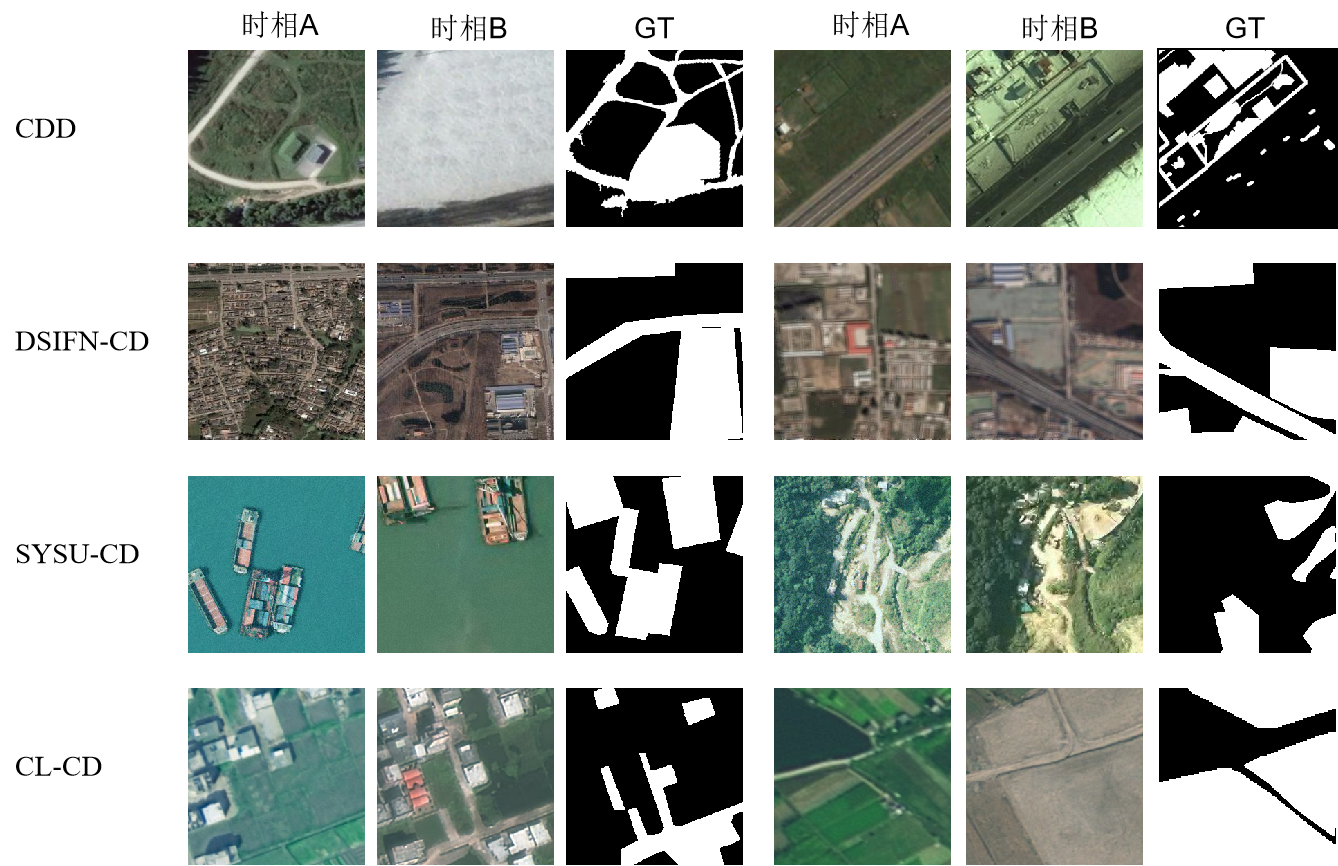
\includegraphics[scale=0.65]{images/mutil_sample.png}
  \caption{
    多类变化检测数据集部分样例图
  }
  \label{fig:mutil_sample}
\end{figure}

\section{本章小结}
本章主要介绍了本文研究内容的相关技术,首先简要介绍了本研究用到的ResNet卷积神经网络,随后阐述了与之相关的Vison Transformer模型的架构和原理。接着大致介绍了本文研究中进行对比实验的几种半监督变化检测SOTA方法。以及实验中使用的变化检测的两种种最常用的评价指标。最后介绍了本文使用的十个公开数据集,所有实验均在这十个数据集上进行训练和验证。
\cleardoublepage
\chapter{基于自适应动态阈值的半监督变化检测算法}
\section{引言}
半监督变化检测方法中基于伪标记和一致性正则化的方法取得了巨大的成功,其关键思想在于模型应该根据半监督学习中的平滑假设和低密度假设,在不同的扰动下对相同的未标记数据产生类似的预测或相同的伪标签。然而,这种方法在利用未标记数据时存在明显局限性。由于它们要么采用固定阈值,要么依赖临时性的阈值调整方案,仅能筛选出部分可信的未标记样本用于训练。更重要的是,这些方法缺乏针对不同数据分布的自适应调整机制,导致模型性能欠佳且收敛速度缓慢。

通常情况下,为保证伪标签的质量,需要设定一个高阈值。然而,固定的高阈值可能导致早期训练阶段的数据利用率低,并且忽略了不同类别的学习难度差异。Dash\cite{xu2021dash}和admatch\cite{berthelot2021adamatch}等半监督学习方法提出随着训练的进行,逐渐增加固定的全局阈值(特定于数据集)。虽然这些方法提高了对未标记数据的利用率,但这种特设阈值调整方案是由超参数进行控制,因此与模型的学习过程脱节。FlexMatch\cite{zhang2021flexmatch}表明,不同的类应该有不同的局部阈值(特定于类别)。虽然局部阈值考虑了不同类别的学习差异,但它们仍然是从预定义的固定全局阈值映射出来的。Adsh\cite{guo2022adash}通过优化每个类的伪标签数量,从预定义的非平衡半监督学习阈值中获得自适应阈值。总而言之,这些方法在根据模型的学习进度调整阈值方面均存在一些不足之处,从而阻碍了训练过程,特别是当标记数据过于稀缺而无法提供足够的监督时。

此外,此前的基于伪标签的半监督变化检测方法中,对于那些被筛选掉的低置信度预测都是直接丢弃,而这样可能造成的问题就是,训练后的模型可能会过度拟合到容易学习的样本上,而忽略了难学习的样本,从而产生“马太效应”,即本来就强的变得更强,本来就弱的变得更弱。

因此,我们认为需要根据模型的学习状态来自适应地确定阈值。具体来说,使用一个较低的全局阈值来利用更多的未标记数据,并在模型早期训练阶段加快收敛速度。随着训练过程的进行,预测置信度不断增加,此时使用更高的全局阈值来过滤掉错误的伪标签来减轻确认偏差。此外,由于变化检测中前景和背景类别的极度不平衡,还应该根据模型对变化和不变类预测的置信度,分别为前景、背景定义一个局部阈值,以减轻类别不平衡带来的预测偏差。并且我们增加了一个低置信度学习模块,旨在最大限度地利用整个未标记数据集,以提高训练过程中的泛化程度。具体来说,我们将来自低置信度预测的软伪标签中可能存在的正确信息通过一致性约束利用起来,以提高模型的性能和表征能力,最终提出了AdTSemiCD(Semi-supervised change detection with an adaptive dynamic thresholding)半监督变化检测框架。

本章介绍了基于自适应动态阈值的半监督变化检测算法——AdTSemICD,首先整体性的阐述了算法的框架和训练流程,随后详细介绍了基于预测概率分布的全局动态阈值和类别动态阈值,以及设计的低置信度学习模块。最后在实验部分报告了本章方法在十个公开数据集上取得的实验结果,从定性和定量两个角度进行了全方位的对比,以及全面的消融实验分析,验证了AdTSemiCD的有效性。
\section{基于自适应动态阈值的半监督变化检测框架}
\subsection{整体框架}
图\ref{fig:AdT_frame}展示了AdTSemiCD的网络框架。半监督变化检测的任务描述如下:给定一个标记数据集$D_{l}=\left\{\left\{x_{a, i}^{l}, x_{b, i}^{l}\right\}, y_{i}^{l}\right\}_{i=1}^{m}$,一个无标注数据集$D_{u}=\left\{x_{a, j}^{u}, x_{b, j}^{u}\right\}_{j=1}^{n}$,其中$\left\{\left\{x_{a, i}^{l}, x_{b, i}^{l}\right\}, y_{i}^{l}\right\}$代表第i个双时相图像对和真实标签,以及$\left\{x_{a, j}^{u}, x_{b, j}^{u}\right\}$代表第i对未标记图像对,下标a和b分别是用于标识双时相图像对的前、后时相的图像,标注数据集和无标注数据集的样本数量分别是n和m, 并且$n \gg m$,模型不仅可以从$D_{l}$中提取有意义的信息,还可以通过利用$D_{u}$中大量未标记的训练样本来捕获更广泛的特征,以提高模型的泛化能力。
\begin{figure}[!htbp]
	\centering
	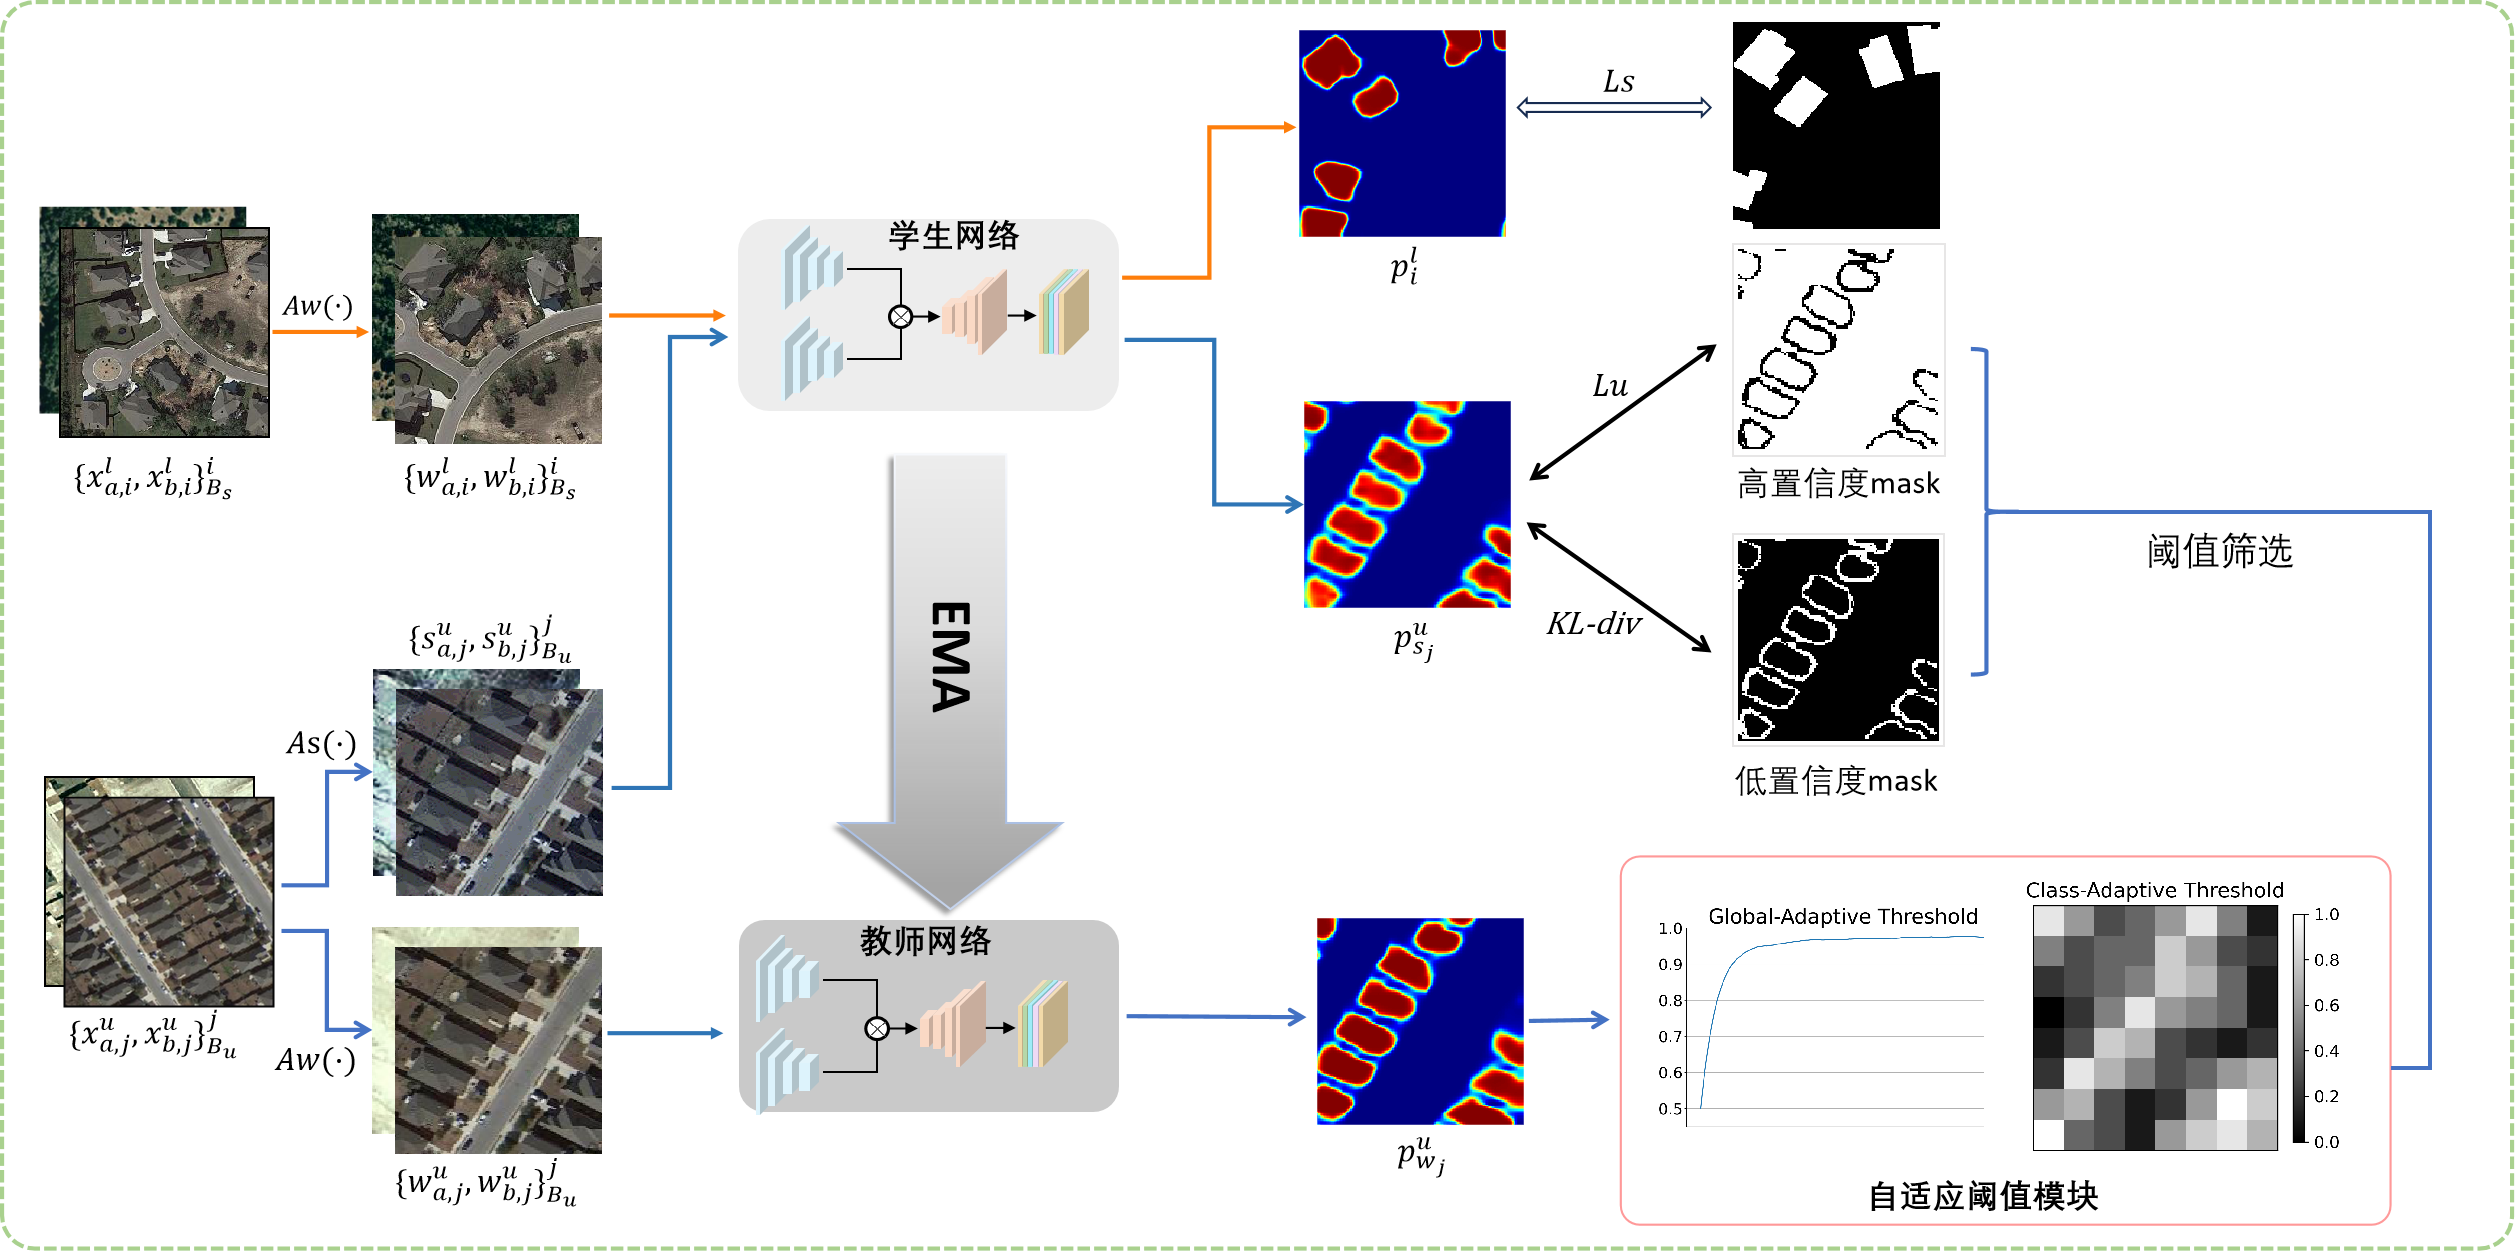
\includegraphics[scale=0.35]{images/AdTFrame.png}
	\caption{
		AdTSemiCD算法的整体框架
	}
	\label{fig:AdT_frame}
\end{figure}

\textbf{模型架构}:在本研究中,我们采用广泛应用的平均师生框架来完成半监督变化检测任务。该网络由两个组件组成,学生模型$M_{stu}$和教师模型$M_{tea}$具有相同的网络结构,分别由$\theta_s$和$\theta_t$参数化。其权重通过梯度下降方法进行优化,训练学生模型从少量标记样本和大量未标记样本中提取变化特征。相反,而教师模型$M_{tea}$用于生成伪标签来指导学生学习未标记的数据,教师模型通过EMA方法更新参数。

无标记样本在输入到教师和学生网络之前会分别经历弱增强$A_{w}(\cdot)$以及进一步的强增强$A_{s}(\cdot)$过程,以提供输出一致性正则化项。

\textbf{训练目标}:目标是最小化模型在$D_{l}$上训练的监督损失$L_s$和在$D_{u}$上训练的无监督损失$L_u$。在训练过程中,样本以随机打乱的小批次(标记样本批次$B_l$和无标记样本批次$B_u$)的形式输入网络。一个小批次内在标记样本上的$L_s$损失计算为模型对其输出的预测概率$P_{i}^{l}$与真实标签$y_{i}^{l}$(Ground Truth,GT)之间的交叉熵(Cross Entropy,CE):
\begin{equation}
  \label{eq:MTLossS}
  \mathcal{L}_{s}=\frac{1}{\left|\mathcal{B}_{l}\right|} \sum_{i=1}^{\left|\mathcal{B}_{l}\right|} \mathrm{CE}\left(p_{i}^{l}, y_{i}^{l}\right)
\end{equation}

其中$\left|\mathcal{B}_{l}\right|$表示标记样本批次的大小,$p_{i}^{l}=M_{stu}^{\theta}\left(x_{a,i}^{l}, x_{b,i}^{l}\right)$表示学生模型对第i对标注图像对的预测概率。

一个批次内在未标记样本上的无监督损失$L_u$也类似,这里我们使用来自$M_{tea}$的伪标签作为监督,因此$L_u$计算为:
\begin{equation}
  \label{eq:MTLossU}
  \mathcal{L}_{u}=\frac{1}{\left|\mathcal{B}_{u}\right|} \sum_{j=1}^{\left|\mathcal{B}_{u}\right|} \mathrm{CE}\left(p_{s, j}^{u}, \hat{y}^{u}_{j}\right),
\end{equation}
\begin{equation}
  \label{eq:MTpesudo}
  \hat{y}^{u}_{j}={\arg \max } \left(p_{w, j}^{u}\right)>\tau
\end{equation}
其中$\left|\mathcal{B}_{u}\right|$表示未标记样本小批次的大小,$p_{w, j}^{u}=M_{t e a}^{\theta}\left(w_{a, j}^{u}, w_{b, j}^{u}\right)$表示教师模型对第i对弱增强未标记图像对的变化的预测概率结果,进一步利用$\arg \max$算子对其进行取最大运算得到伪标签$\hat{y}^{u}_{j}$,如公式\ref{eq:MTpesudo}所示,$p_{s, j}^{u}=M_{s t u}^{\theta}\left(s_{a, j}^{u}, s_{b, j}^{u}\right)$表示教师模型对第i对强增强未标记图像对的变化检测预测概率,$\tau$为固定的筛选阈值,用于剔除低置信的预测。

综上所述,AdaSemiCD训练过程总的损失为:
\begin{equation}
  \label{eq:EMALoss}
  \mathcal{L}=\mathcal{L}_{s}+\lambda(\cdot) \mathcal{L}_{u}
\end{equation}

在本研究中,为了加快模型收敛速度,与以往的研究\cite{sohn2020fixmatch}\cite{transformation_medical}保持一致,$\lambda(\cdot)$采用固定超参数表示。

\textbf{训练策略}:学生网络的参数$\theta$通过随机梯度下降(SGD)技术最小化总训练损失来优化,以最小化总体损失$\mathcal{L}$。而教师网络的参数$\theta'$通过学生模型参数$\theta$在训练时间序列上的指数移动平均来更新,如\ref{eq:ema}所示。超参数$\beta$作为动量参数,$\beta$值越大,移动指数平均的窗口越宽。通常,$\beta$选择接近1.0的数字,例如在本研究中,选择0.996。
\begin{equation}
  \label{eq:ema}
  \theta^{\prime}=\beta \theta^{\prime}+(1-\beta) \theta
\end{equation}

\textbf{问题定义}:
监督学习过程即通过最小化学生模型预测概率与真实样本标签之间的交叉熵损失来优化模型的参数;无监督学习过程通常情况下将教师模型的输出作为训练指导,对于教师模型在无标记样本上的输出概率,通过一个阈值来筛选出可信的预测作为伪标签,然后最小化学生模型输出概率和伪标签之间的交叉熵损失来优化学生模型的参数。教师模型的参数更新则由学生模型参数的移动指数平均累计得到。此外通常情况下,在此框架中还引入了一致性正则化,即对无标记样本分别进行弱增强以及在此之上的进一步的强增强,分别作为教师模型和学生模型的输入,基于低密度假设和平滑假设,二者的输出结果应该保持一致。通过一致性正则化,能够进一步提高模型的泛化能力。

很明显,生成伪标签过程中的阈值筛选是一个非常重要的过程,阈值过高会导致对无标记数据的利用率不足,而阈值过低又会导致引入错误标签。并且对于不同数据分布,最佳阈值的选择往往不相同,需要通过实验来验证。因此,我们设计了一种自适应的动态阈值调整机制,根据模型在不同数据上的预测概率分布,动态更新模型对于前景和背景的概率筛选阈值,即公式\ref{eq:pesudo}中的$\tau$为自适应动态改变的。此外,还设计了一个额外的低置信度学习模块,进一步提高对无标记数据的利用率。我们将在下面的小节中分别对这些设计进行详细阐述。
\subsection{全局自适应阈值}
在我们的自适应阈值机制中,首先估计一个全局阈值作为模型置信度的均线。当训练开始时,阈值较低,此时接受更多可能正确的样本进入训练以加快模型的收敛速度。随着模型预测变得更加自信,全局阈值自适应地增加,以过滤掉可能不正确的样本,减少确认偏差。
\begin{figure}[htb]
  \centering
  \hspace*{\fill} % 左侧留空
  \begin{subfigure}[t]{0.46\textwidth} % 左图占45%宽度
      \centering
      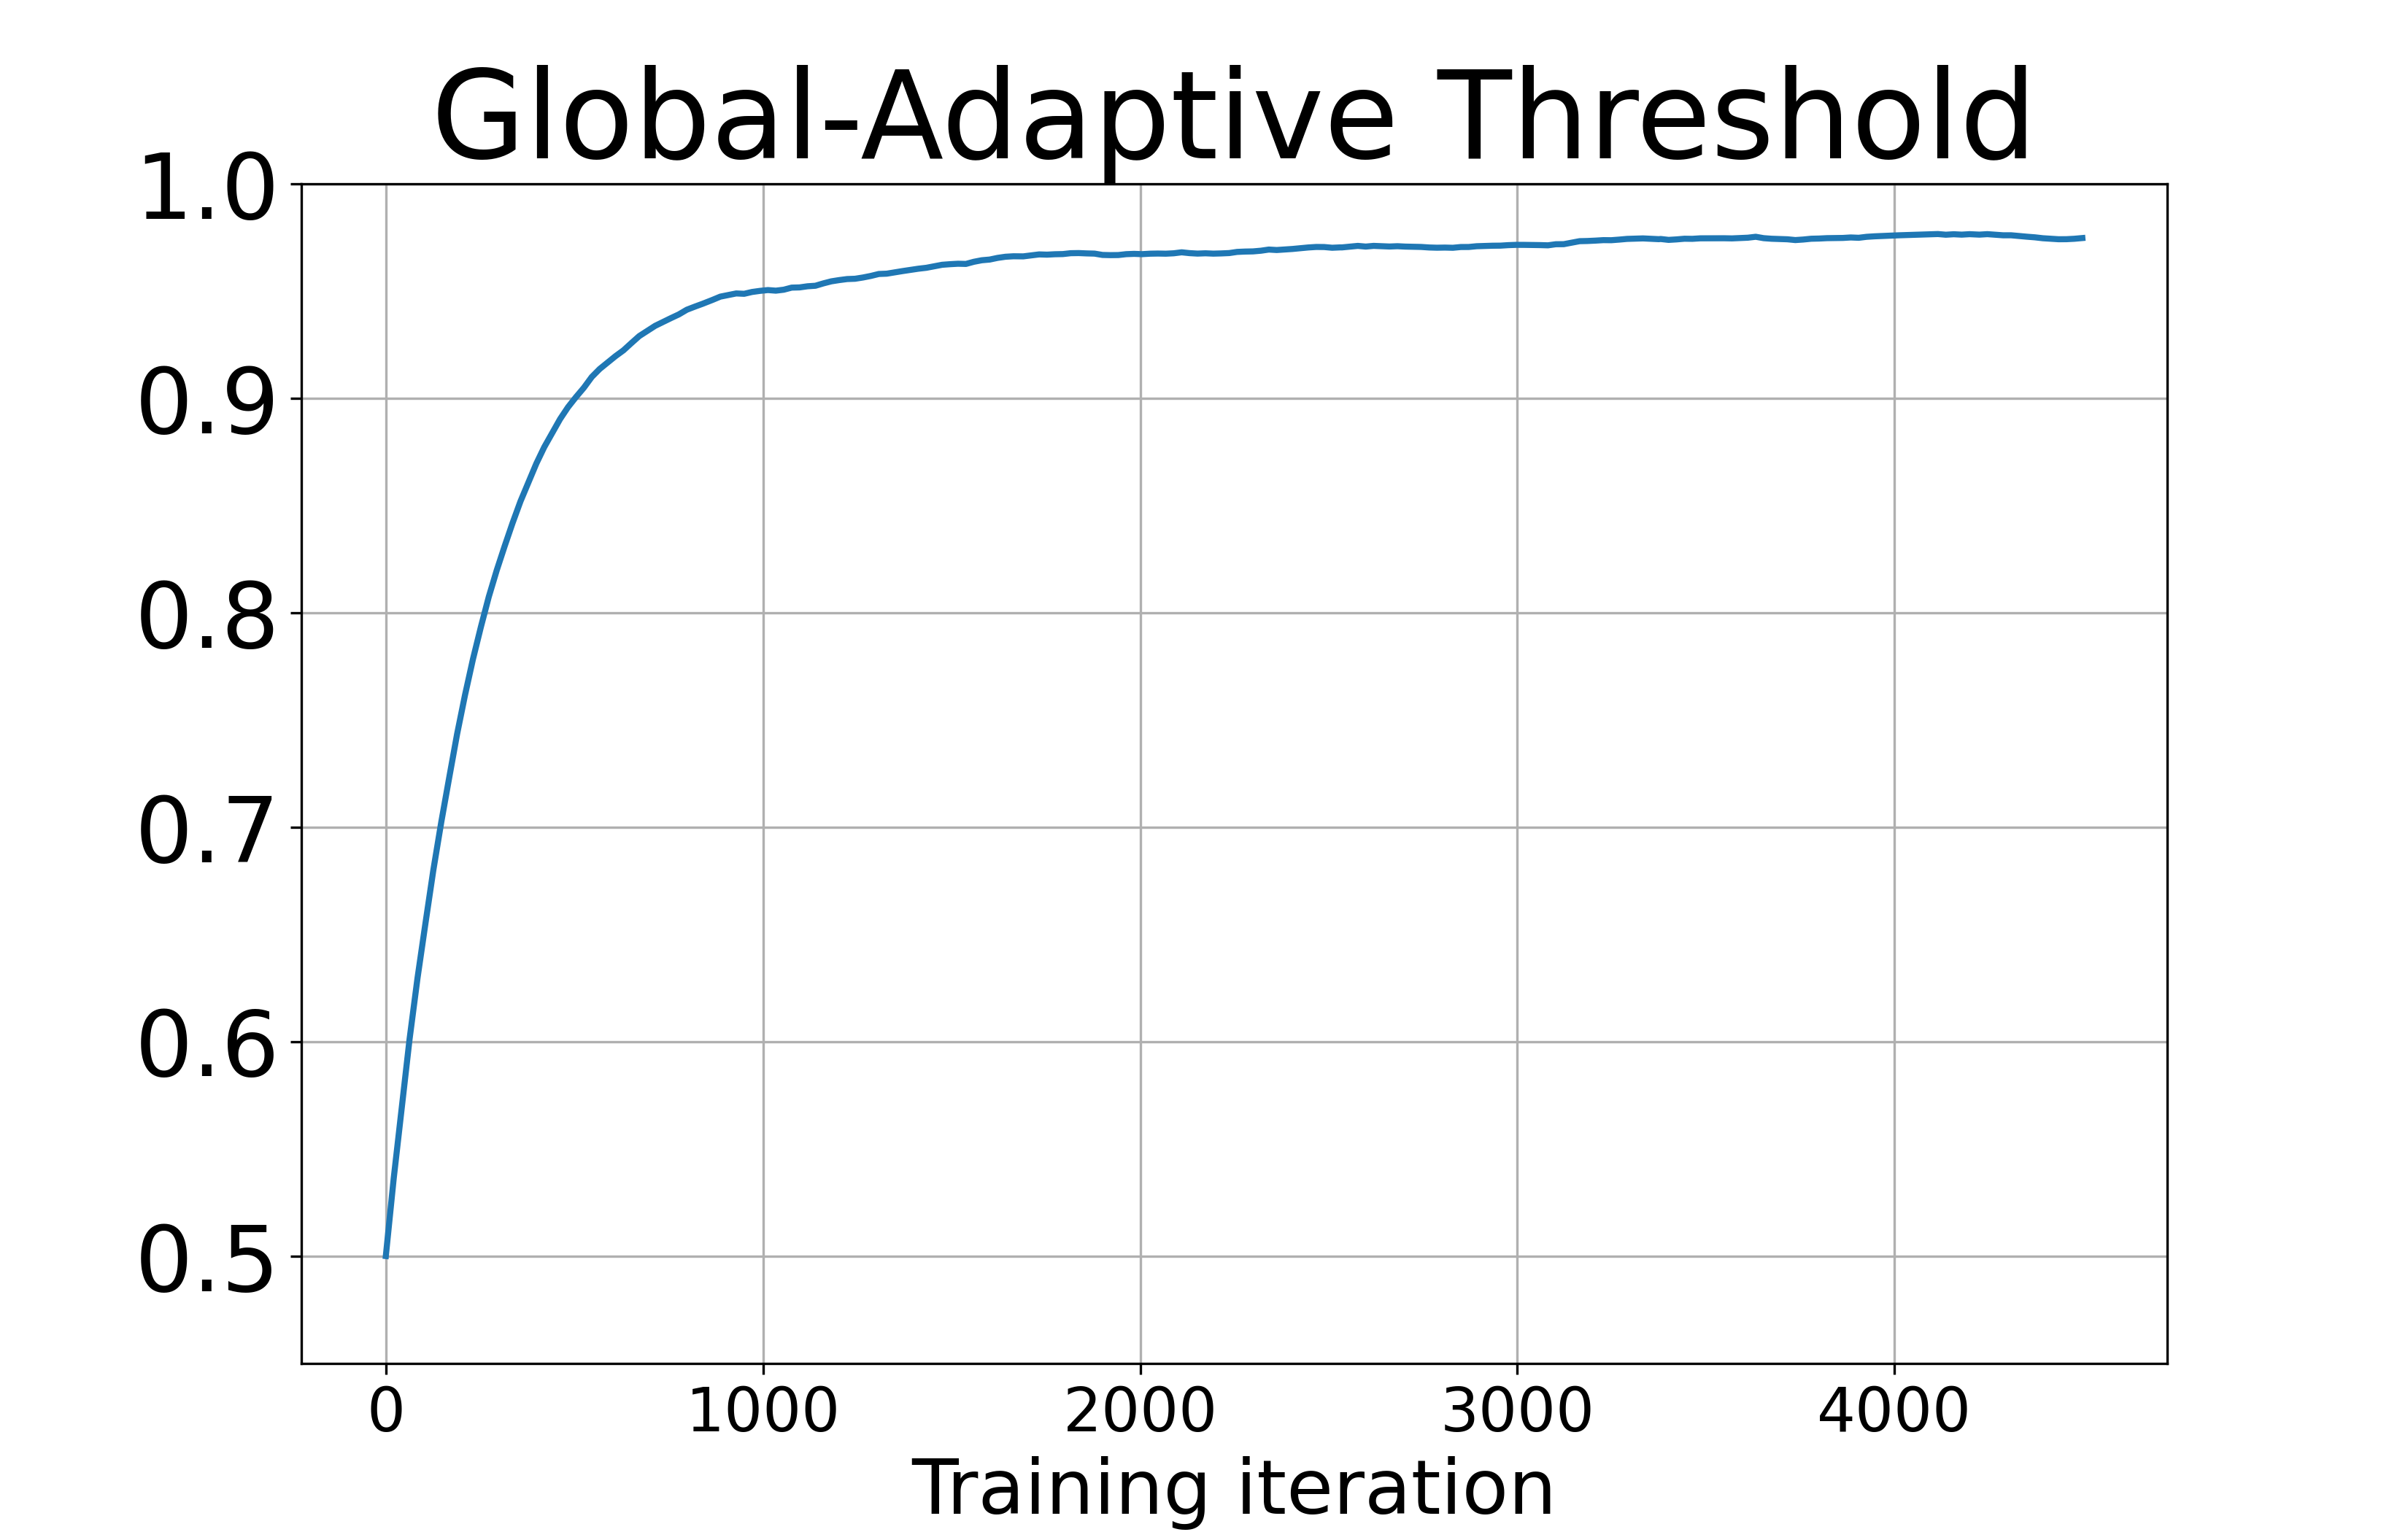
\includegraphics[scale=0.27]{images/adath_plot.png}
      \caption{全局自适应阈值}
      \label{fig:globalTh_left}
  \end{subfigure}
  \hfill % 两图之间留空
  \begin{subfigure}[t]{0.46\textwidth} % 右图占45%宽度
      \centering
      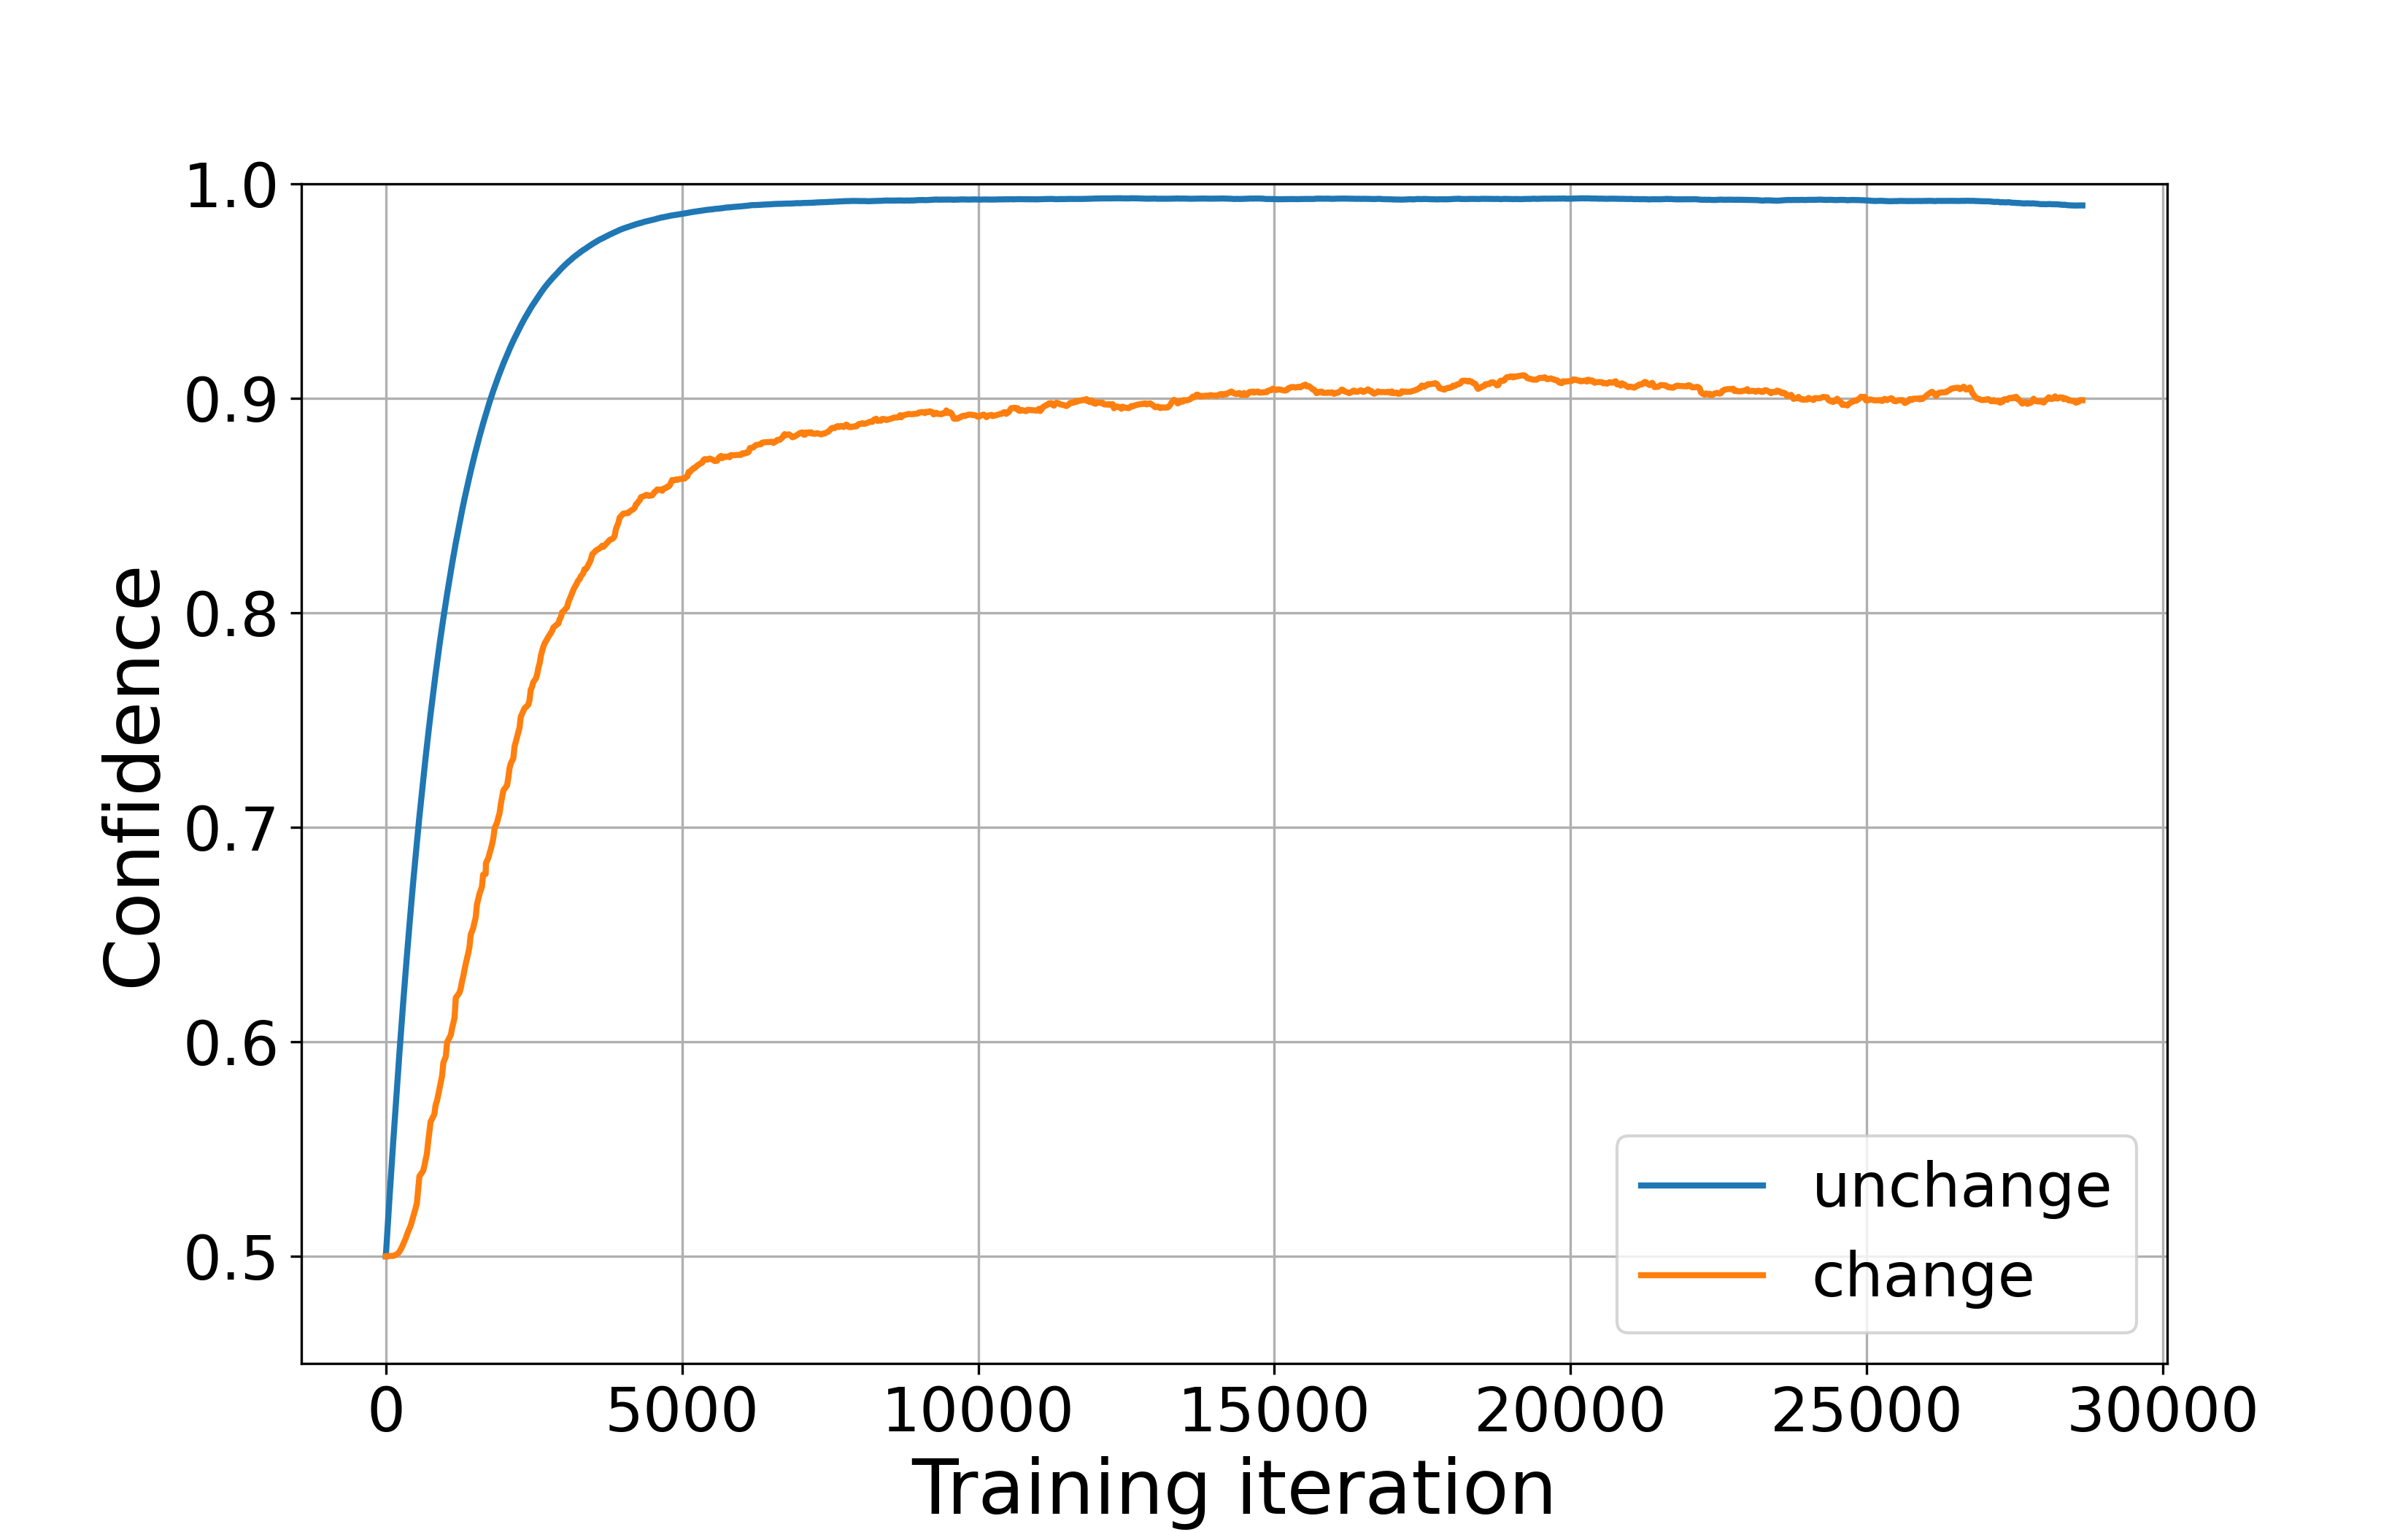
\includegraphics[scale=0.27]{images/prob_ema.png} % 替换为右图路径
      \caption{两种类别的预测置信度} % 修改为右图的标题
      \label{fig:classTh_right}
  \end{subfigure}
  \hspace*{\fill} % 左侧留空
  \caption{训练过程中的全局阈值和两种类别的置信度变化情况}
  \label{fig:AdaTh_combined}
\end{figure}
具体说来,我们基于以下两个原则设计全局阈值。首先,全局阈值应该与模型对未标记数据预测的概率分布相关,要尽可能地反映模型的整体学习状况。此外,全局阈值应该在训练过程中稳定地增加,以确保丢弃错误的伪标签。考虑到以上两点,我们将全局阈值$\tau_t$设置为模型对未标记数据的平均置信度,其中$t$表示第$t$个迭代轮次。为了使得阈值保持平滑,我们将全局置信度估计为每个训练时间步的置信度的指数移动平均(EMA),并且在训练初始时间将全局阈值设置为每种类别的平均预测概率,即0.5。综上,全局动态阈值的计算公式如\ref{eq:Adath_global}所示:
\begin{equation}
    \label{eq:Adath_global}
    \tau_{t}=\left\{\begin{array}{ll}
      0.5, & \text { if } t=0 \\
      \beta \tau_{t-1}+(1-\beta) \frac{1}{\left|\mathcal{B}_{u}\right|} \sum_{b=1}^{\left|\mathcal{B}_{u}\right|} \max \left(p_{w, j}^{u}\right), & \text { otherwise }
      \end{array}\right.
\end{equation}

其中,$p_{w, j}^{u}$为教师模型在弱增强输入图像上的预测概率输出,$\beta$与公式\ref{eq:ema}中一致,为EMA的衰减动量。
\subsection{类别自适应阈值}
如图\ref{fig:Adasemicd_imbalance}所示,变化检测任务存在严重的类别失衡问题,模型在背景类别上的预测必然更加自信。类别动态阈值旨在以特定于前景变化类别和背景不变类的方式调节各自的阈值,以考虑类内多样性和两种类别的差异性。我们分别计算模型对两种类别的预测概率分布的期望,以此来估计模型特定于类别的学习状态,具体地说,就是基于模型特定于类别的平均置信度,动态调整全局置信度在每个类别上的表示。同样地,我们也是将类别平均置信度估计为在每个训练时间步的置信度的指数移动平均(EMA),并且在训练初始时间将类别置信度设置为一个均匀分布,即(0.5,0.5)。计算公式如下:
\begin{figure}[htb]
  \centering
  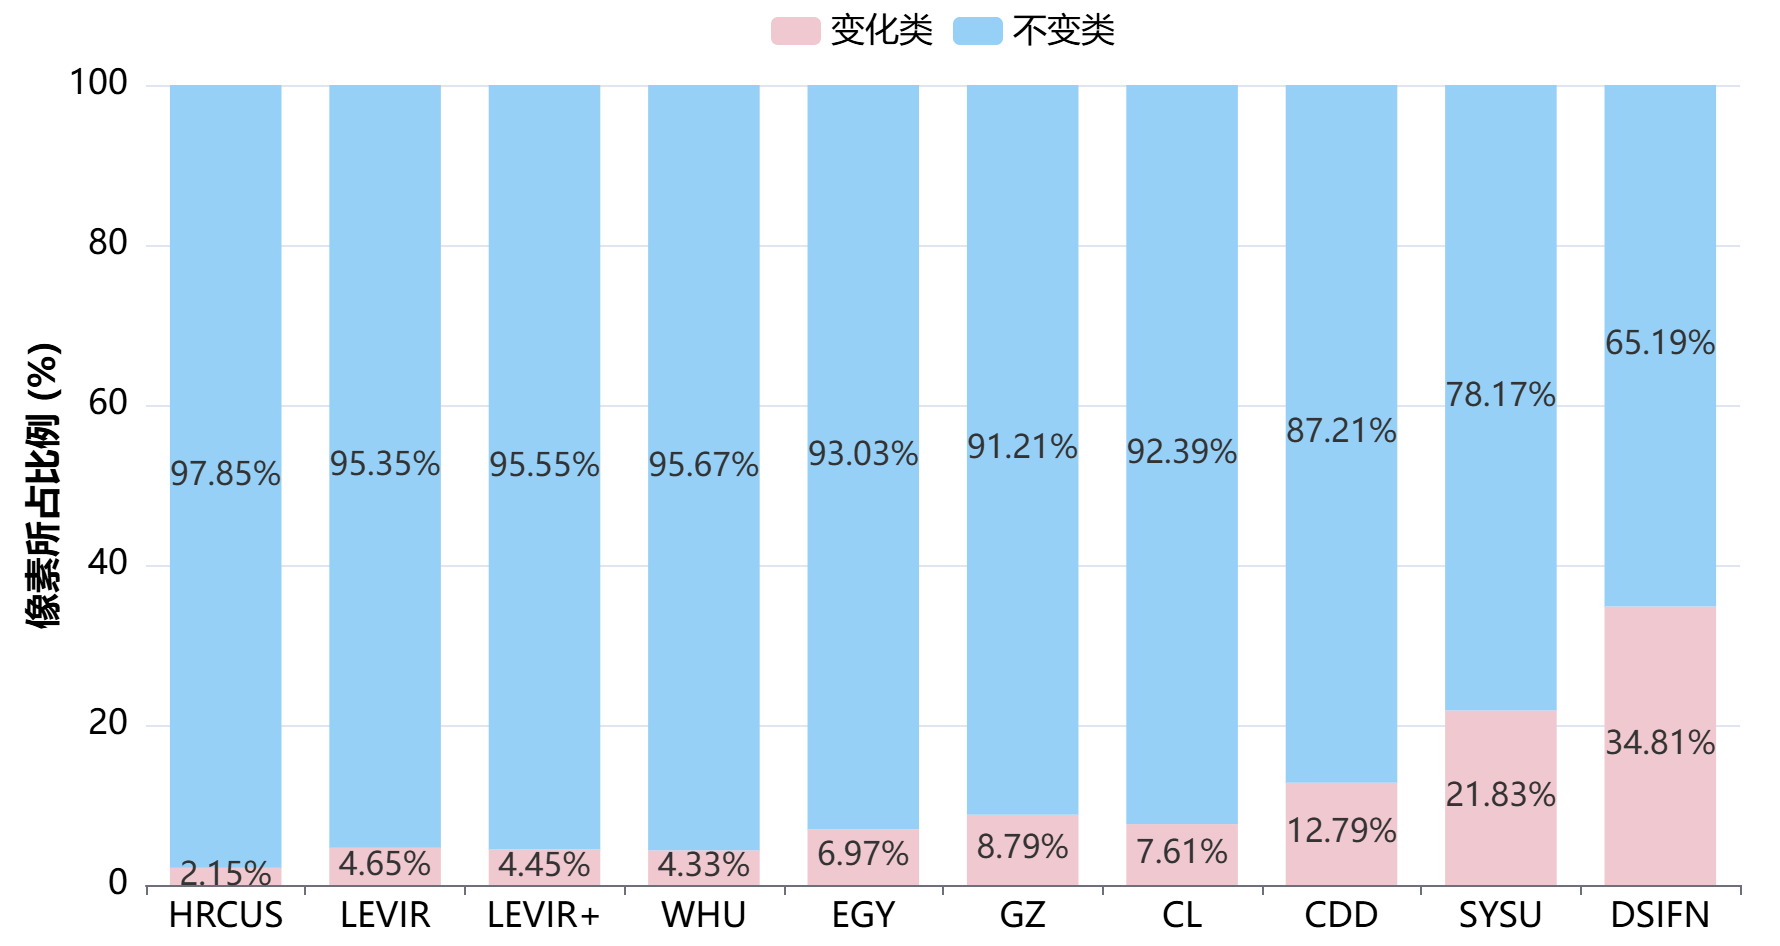
\includegraphics[scale=0.25]{images/imbalance.png}
  \caption{
    公开变化检测数据集的类别不平衡统计
  }
  \label{fig:Adasemicd_imbalance}
\end{figure}
\begin{equation}
    \label{eq:Adath_pmodel}
    \tilde{p}_{t}(c)=\left\{\begin{array}{ll}
      0.5, & \text { if } t=0 \\
      \lambda \tilde{p}_{t-1}(c)+(1-\lambda) \frac{1}{\left|\mathcal{B}_{u}\right|} \sum_{b=1}^{\left|\mathcal{B}_{u}\right|} p_{w, j}^{u}(c), & \text { otherwise }
      \end{array}\right.
\end{equation}

其中$\tilde{p}_{t} = [\tilde{p}_{t}[0], \tilde{p}_{t}[1]]$是包含前景和背景类别的预测概率分布的期望。然后对其进行一个最大归一化,将归一化后的值作为类别阈值权重,最终特定于类别的自适应动态阈值结合了全局动态阈值和类别置信度期望,公式表示为:
\begin{equation}
  \label{eq:Adath_weight}
  \mathcal{W}(c)=\frac{\tilde{p}_{t}(c)}{\max \left\{\tilde{p}_{t}(c): c \in[0, 1]\right\}},
\end{equation}
\begin{equation}
  \label{eq:Adath_localTh}
  \tau_{t}(c)=\mathcal{W}(c) \times \tau_{t}
\end{equation}

则式\ref{eq:MTLossU}中的伪标签$\hat{y}_{i}^{u}$的筛选机制被优化为:
\begin{equation}
  \label{eq:Adath_argmax}
  \hat{y}_{i}^{u}=p_{w, j}^{u}(\arg \max \left(p_{w, j}^{u} \right)) \ge \tau_{t}\left(\arg \max \left(p_{w, j}^{u} \right)\right),
\end{equation}
\subsection{低置信度学习}
在上一步的筛选过程中,剔除掉了许多低置信度的标签,仅使用高置信度的预测作为硬伪标签。这一做法基于这样一种假设:高置信度的标签都是正确的,而低置信度的标签都是错误的。但是我们在研究中发现,被筛选掉的一部分低置信度标签中也包含着正确的标签信息,但是在模型学习过程中没有得到充分的利用。因此我们将这部分低置信的标签并不完全丢弃,而是将其作为软伪标签,利用强弱增强图像对之间的输出一致性正则化对其进行学习。具体地,我们使用KL散度作为低置信度学习的损失函数,计算公式如下:
\begin{equation}
  \label{eq:Adath_lossSoft}
  \mathcal{L}_{\mathrm{KL}}=\frac{1}{\left|\mathcal{B}_{u}\right|} \sum_{b=1}^{\left|\mathcal{B}_{u}\right|}D_{\mathrm{KL}}\left(p_{s, j}^{u}, p_{w, j}^{u}\right) \cdot \left(p_{w, j}^{u}(\arg \max \left(p_{w, j}^{u} \right))<\tau_{t}\left(\arg \max \left(p_{w, j}^{u}\right)\right)\right)
\end{equation}

综上,我们的AdTSemiCD的总体损失被重新定义为:
\begin{equation}
  \label{eq:Adath_losstotal}
  \mathcal{L}_{total}=\mathcal{L}_{s}+\lambda_{u} \mathcal{L}_{u}+\lambda_{k} \mathcal{L}_{KL}
\end{equation}

$\lambda_{u}$和$\lambda_{k}$分别是硬标签交叉熵损失和软标签KL散度损失的权重超参数,我们会在消融实验部分对其取值选择进行探究。
\begin{figure}[htb]
  \centering
  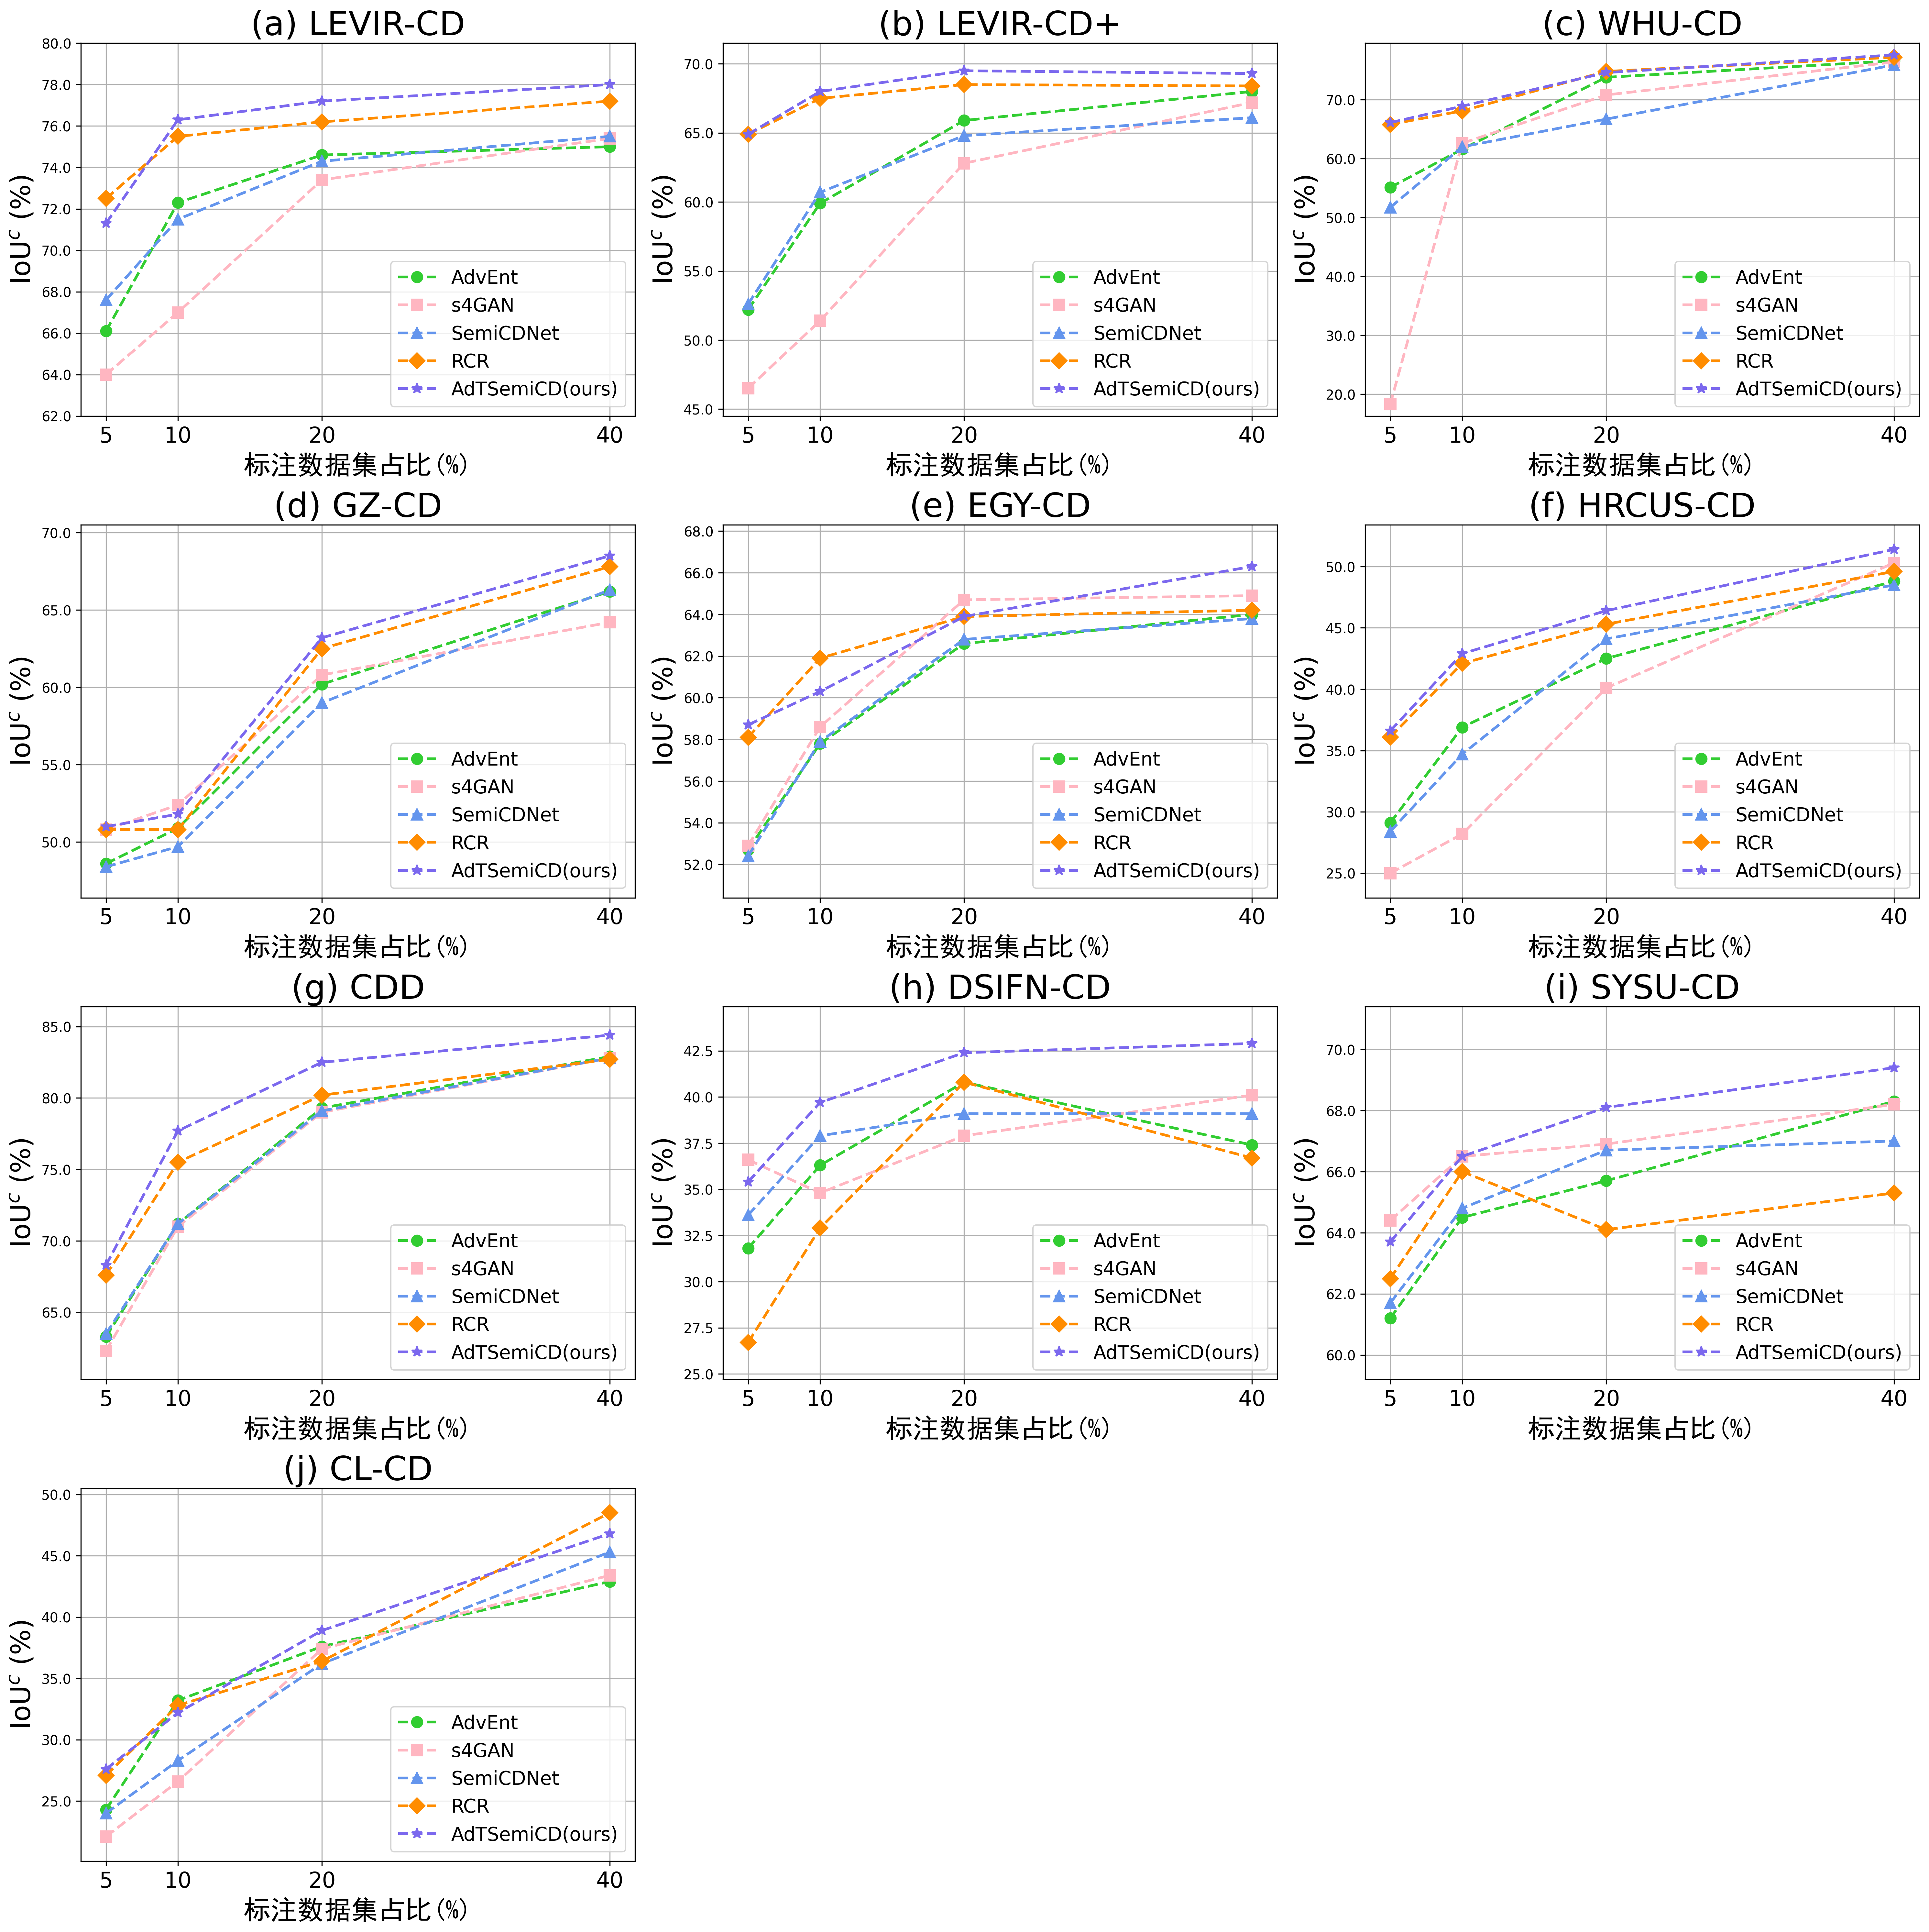
\includegraphics[scale=0.30]{images/AdTvis_plot.png}
  \caption{
    AdTSemiCD与SOTA方法在10个数据集上的性能对比折线图
  }
  \label{fig:AdTiou_plot}
\end{figure}
\section{实验结果及分析}
\textbf{数据划分}:我们对所有数据集遵循相同的划分规则,定义了四种半监督设置,我们分别选择训练集中5$\%$,10$\%$,20$\%$和40$\%$作为标记样本训练集,训练集中其他样本均视作无标记样本,在训练过程中不使用任何真实标注信息。其中在LEVIR-CD和WHU-CD两个数据集上我们遵循\cite{bandara2022RCR}\cite{Zhang2023FPA}中现有的半监督划分,在其他数据集上我们进行了随机划分,但在所有方法的对比实验上我们都是使用此相同的训练样本集,以进行公平和科学的实验对比。

\textbf{实现细节}:为了防止网络结构带来的性能差异影响我们的结论,我们所有对比方法均使用ResNet50+PPM网络作为我们的变化检测网络。我们将初始学习率设置为0.01,它以0.9的动量随训练进程逐渐线性降低到1e-4,并使用SGD优化器训练所有方法。所有的模型都进行了80个epoch的训练,每个批次的标记和未标记每次迭代的小批次大小均设置为8。此外,所采用的弱增强包括随机翻转、随机缩放、随机裁剪,强增强包括\cite{cubuk2020randaugment}中引用的9种强增强方式。此外,对于全局动态阈值,我们设定了与对比试验中固定阈值(0.95)一样的上限,到达上限之后就保持此阈值不再变化。所有的实验均利用PyTorch框架实现并且在4块Tesla V100-SXM2-32GB GPU上进行模型训练和验证。
\subsection{对比试验}
我们与RCR等几种半监督变化检测算法和s4GAN等半监督语义分割方法进行了全方位的对比实验,包括以$IoU^c$和$OA$为指标的定量实验结果对比,以及在每个数据集的测试集上的推理结果可视化对比,并且AdTSemiCD都取得了优异的结果。
\subsubsection{定量对比}
\begin{table}[!htbp]
  \centering
  % \tiny
  \scriptsize
  \caption{不同CD方法在二值建筑物变化检测数据集上的平均定量性能对比}
  \resizebox{0.9\textwidth}{!}{
  \begin{tabular}{p{20mm}p{25mm}p{8mm}p{8mm}cp{8mm}p{8mm}cp{8mm}p{8mm}cp{8mm}p{8mm}} %
      \toprule
      \multirow{2}{*}{数据集} & \multirow{2}{*}{方法} & \multicolumn{2}{c}{5\%} & & \multicolumn{2}{c}{10\%} & & \multicolumn{2}{c}{20\%} & & \multicolumn{2}{c}{40\%}\\
      \cmidrule{3-4} \cmidrule{6-7} \cmidrule{9-10} \cmidrule{12-13}
      & & {$IoU^c$} & {OA} && {$IoU^c$} & {OA} & & {$IoU^c$} & {OA} &&{$IoU^c$} & {OA}\\
      \midrule
      \multirow{8}{*}{LEVIR-CD}
      & 仅监督   &   61.0 & 97.60 && 66.8 & 98.13 && 72.3 & 98.44 && 74.9 & 98.60 \\ %40
      & AdvEnt\cite{vu2019advent}& 66.1 & 98.08 && 72.3 & 98.45 && 74.6 & 98.58 && 75.0 & 98.60 \\ %40
      & s4GAN\cite{mittal2019semi}& 64.0 & 97.89 && 67.0 & 98.11 && 73.4 & 98.51 && 75.4 & 98.62 \\
      & SemiCDNet\cite{peng2021SemiCDNet} & 67.6 & 98.17 && 71.5 & 98.42 && 74.3 & 98.58 && 75.5 & 98.63 \\ %40
      & RCR\cite{bandara2022RCR}& \cellcolor{mycyan}\textbf{72.5} & \cellcolor{mycyan}\textbf{98.47} && \underline{75.5} & \underline{98.63} && \underline{76.2} & \underline{98.68} && \underline{77.2} & \underline{98.72} \\
      \rowcolor{mycyan}
      \multirow{-8}{*}{\cellcolor{white}}& \cellcolor{white}AdTSemiCD   &   \cellcolor{white}\underline{71.3} & \cellcolor{white}\underline{98.40} && \textbf{76.3} & \textbf{98.66} && \textbf{77.2} & \textbf{98.75} && \textbf{78.0} & \textbf{98.79} \\%40
      \cline{2-13}
      & Oracle & \multicolumn{11}{c}{$ IoU^c$=\textcolor{red}{\bf 77.9} and OA=\textcolor{red}{\bf 98.77}} \\
      \bottomrule
      %\midrule
      \multirow{8}{*}{LEVIR-CD+}
      & 仅监督   &   52.0 & 97.72 && 58.4 & 98.06 && 66.1 & 98.31 && 66.2 & 98.42 \\ %40
      & AdvEnt\cite{vu2019advent}& 52.2 & 97.68 && 59.9 & 98.11 && 65.9 & 98.37 && 68.0 & 98.51 \\ %40
      & s4GAN\cite{mittal2019semi}& 46.5 & 97.25 && 51.4 & 97.66 && 62.8 & 98.18 && 67.2 & 98.46 \\
      & SemiCDNet\cite{peng2021SemiCDNet} & 52.6 & 97.66 && 60.7 & 98.24 && 64.8 & 98.37 && 66.1 & 98.38 \\ %40
      & RCR\cite{bandara2022RCR}& \underline{64.9} & \underline{98.25} && \underline{67.5} & \underline{98.45} && \underline{68.5} & \underline{98.52} && \underline{68.4} & \underline{98.51} \\
      \rowcolor{mycyan}
      \multirow{-8}{*}{\cellcolor{white}}& \cellcolor{white}AdTSemiCD   &   \textbf{64.9} & \textbf{98.26} && \textbf{68.0} & \textbf{98.48} && \textbf{69.5} & \textbf{98.59} && \textbf{69.3} & \textbf{98.60} \\%40
      \cline{2-13}
      & Oracle & \multicolumn{11}{c}{$ IoU^c$=\textcolor{red}{\bf 70.5} and OA=\textcolor{red}{\bf 98.63}} \\
      \bottomrule
      % \midrule
      \multirow{8}{*}{WHU-CD}
      & 仅监督   &   50.0 & 97.48 && 55.7 & 97.53 && 65.4 & 98.20 && 76.1 & 98.94 \\ %40
      & AdvEnt\cite{vu2019advent}& 55.1 & 97.90 && 61.6 & 98.11 && 73.8 & 98.80 && 76.6 & 98.94 \\ %40
      & s4GAN\cite{mittal2019semi}& 18.3 & 96.69 && 62.6 & 98.15 && 70.8 & 98.60 && 76.4 & 98.96 \\
      & SemiCDNet\cite{peng2021SemiCDNet} & 51.7 & 97.71 && 62.0 & 98.16 && 66.7 & 98.28 && 75.9 & 98.93 \\ %40
      & RCR\cite{bandara2022RCR}& \underline{65.8} & \underline{98.37} && \underline{68.1} & \underline{98.47} && \cellcolor{mycyan}\textbf{74.8} & \cellcolor{mycyan}\textbf{98.84} && \underline{77.2} & \underline{98.96} \\
      \rowcolor{mycyan}
      \multirow{-8}{*}{\cellcolor{white}}& \cellcolor{white}AdTSemiCD   &   \textbf{66.1} & \textbf{98.41} && \textbf{68.9} & \textbf{98.54} && \cellcolor{white}\underline{74.6} & \cellcolor{white}\underline{98.83} && \textbf{77.6} & \textbf{99.03} \\%40
      \cline{2-13}
      & Oracle & \multicolumn{11}{c}{$ IoU^c$=\textcolor{red}{\bf 85.5} and OA=\textcolor{red}{\bf 99.38}} \\
      \bottomrule
      % \midrule
      \multirow{8}{*}{GZ-CD}
      & 仅监督   &   47.5 & 93.56 && 51.4 & 94.26 && 58.0 & 95.65 && 66.3 & \underline{96.62} \\ %40
      & AdvEnt\cite{vu2019advent}& 48.6 & \underline{94.39} && 50.9 & 94.89 && 60.2 & 95.79 && 66.2 & 96.58 \\ %40
      & s4GAN\cite{mittal2019semi}& \underline{50.8} & 94.38 && \cellcolor{mycyan}\textbf{52.4} & \cellcolor{mycyan}\textbf{94.98} && 60.8 & 95.94 && 64.2 & 96.39 \\
      & SemiCDNet\cite{peng2021SemiCDNet} & 48.4 & 93.58 && 49.7 & 94.79 && 59.0 & 95.66 && 66.3 & 96.57 \\ %40
      & RCR\cite{bandara2022RCR}& \underline{50.8} & 93.82 && 50.8 & 94.69 && \underline{62.5} & \underline{96.07} && \underline{67.8} & 96.61 \\
      \rowcolor{mycyan}
      \multirow{-8}{*}{\cellcolor{white}}& \cellcolor{white}AdTSemiCD   &   \cellcolor{mycyan}\textbf{51.0} & \cellcolor{mycyan}\textbf{94.47} && \cellcolor{white}\underline{51.8} & \cellcolor{white}\underline{94.93} && \cellcolor{mycyan}\textbf{63.2} & \textbf{96.26} && \textbf{68.5} & \textbf{96.81} \\%40
      \cline{2-13}
      & Oracle & \multicolumn{11}{c}{$ IoU^c$=\textcolor{red}{\bf 69.0} and OA=\textcolor{red}{\bf 96.93}} \\
      \bottomrule
      \multirow{8}{*}{EGY-CD}
      & 仅监督   &   49.8 & 95.73 && 54.6 & 96.38 && 61.4 & 96.83 && \underline{65.1} & 97.25 \\ %40
      & AdvEnt\cite{vu2019advent}& 52.7 & 96.01 && 57.8 & 96.58 && 62.6 & 96.86 && 64.0 & 97.19 \\ %40
      & s4GAN\cite{mittal2019semi}& 52.9 & 95.94 && 58.6 & 96.50 && \cellcolor{mycyan}\textbf{64.7} & \cellcolor{mycyan}\textbf{97.09} && 64.9 & \underline{97.27} \\
      & SemiCDNet\cite{peng2021SemiCDNet} & 52.4 & 96.00 && 57.9 & 96.31 && 62.8 & 96.95 && 63.8 & 97.19 \\ %40
      & RCR\cite{bandara2022RCR}& \underline{58.1} & \underline{96.50} && \underline{59.9} & \underline{96.77} && \underline{63.9} & \underline{97.08} && 64.2 & 97.18 \\
      \rowcolor{mycyan}
      \multirow{-8}{*}{\cellcolor{white}}& \cellcolor{white}AdTSemiCD   &   \textbf{58.7} & \textbf{96.55} && \textbf{60.3} & \textbf{96.80} && \cellcolor{white}\underline{63.9} & \cellcolor{white}97.05 && \textbf{66.3} & \textbf{97.41} \\%40
      \cline{2-13}
      & Oracle & \multicolumn{11}{c}{$ IoU^c$=\textcolor{red}{\bf 67.6} and OA=\textcolor{red}{\bf 97.54}} \\
      \bottomrule
      \multirow{8}{*}{HRCUS-CD}
      & 仅监督   &   29.5 & 98.11 && 36.0 & 98.45 && 43.4 & 98.68 && 48.9 & 98.84 \\ %40
      & AdvEnt\cite{vu2019advent}& 29.1 & 98.11 && 36.9 & 98.40 && 42.5 & 98.61 && 48.8 & 98.71 \\ %40
      & s4GAN\cite{mittal2019semi}& 25.0 & 97.86 && 28.2 & 98.24 && 40.1 & 98.62 && \underline{50.3} & \underline{98.85} \\
      & SemiCDNet\cite{peng2021SemiCDNet} & 28.4 & 98.00 && 34.7 & 98.44 && 44.1 & 98.68 && 48.5 & 98.74 \\ %40
      & RCR\cite{bandara2022RCR}& \underline{36.1} & \underline{98.36} && \underline{42.1} & \underline{98.69} && \underline{45.3} & \underline{98.76} && 49.6 & 98.66 \\
      \rowcolor{mycyan}
      \multirow{-8}{*}{\cellcolor{white}}& \cellcolor{white}AdTSemiCD   &  \textbf{36.6} & \cellcolor{mycyan}\textbf{98.43} && \textbf{42.9} & \textbf{98.72} && \textbf{46.4} & \textbf{98.81} && \textbf{51.4} & \textbf{98.85} \\%40
      \cline{2-13}
      & Oracle & \multicolumn{11}{c}{$ IoU^c$=\textcolor{red}{\bf 59.0} and OA=\textcolor{red}{\bf 99.06}} \\
      \bottomrule
  \end{tabular}
  }
  \label{tab:AdT-building}
\end{table}
表\ref{tab:AdT-building}和表\ref{tab:AdT-mutil}分别展示了我们在六个二值建筑物变化检测数据集和四个多类别变化检测数据集上的定量实验结果,其中蓝色高亮标注并且加粗显示的数值为最优结果,下划线标注的数值为次优结果。此外,Oracle表示在整个训练数据集上以100$\%$标注率进行训练的结果,为我们对比的上界。
\begin{table}[!htbp]
  \centering
  % \tiny
  \scriptsize
  \caption{不同CD方法在多类变化检测数据集上的平均定量性能对比}
  \resizebox{0.9\textwidth}{!}{
     \begin{tabular}{p{20mm}p{25mm}p{8mm}p{8mm}cp{8mm}p{8mm}cp{8mm}p{8mm}cp{8mm}p{8mm}} %
      \toprule
      \multirow{2}{*}{数据集} & \multirow{2}{*}{方法} & \multicolumn{2}{c}{5\%} & & \multicolumn{2}{c}{10\%} & & \multicolumn{2}{c}{20\%} & & \multicolumn{2}{c}{40\%}\\
      \cmidrule{3-4} \cmidrule{6-7} \cmidrule{9-10} \cmidrule{12-13}
      & & {$IoU^c$} & {OA} && {$IoU^c$} & {OA} & & {$IoU^c$} & {OA} &&{$IoU^c$} & {OA}\\
      \midrule
      \multirow{8}{*}{CDD-CD}
      & 仅监督   &   60.4 & 94.25 && 67.9 & 95.46 && 75.6 & 96.59 && 82.3 & 97.56 \\ %40
      & AdvEnt\cite{vu2019advent}& 63.3 & 94.65 && 71.2 & 96.01 && 79.3 & 97.14 && \underline{82.9} & \underline{97.66} \\ %40
      & s4GAN\cite{mittal2019semi}& 62.3 & 94.69 && 71.0 & 95.94 && 79.0 & 97.10 && 82.8 & 97.63 \\
      & SemiCDNet\cite{peng2021SemiCDNet} & 63.5 & 94.68 && 71.2 & 95.99 && 79.1 & 97.13 && 82.8 & 97.63 \\ %40
      & RCR\cite{bandara2022RCR}& \underline{67.6} & \underline{95.40} && \underline{75.5} & \underline{96.57} && \underline{80.2} & \underline{97.26} && 82.7 & 97.61 \\
      \rowcolor{mycyan}
      \multirow{-8}{*}{\cellcolor{white}}& \cellcolor{white}AdTSemiCD   &   \textbf{68.3} & \textbf{95.52} && \textbf{77.7} & \textbf{96.92} && \textbf{82.5} & \textbf{97.54} && \textbf{84.4} & \textbf{97.77} \\%40
      \cline{2-13}
      & Oracle & \multicolumn{11}{c}{$ IoU^c$=\textcolor{red}{\bf 87.8} and OA=\textcolor{red}{\bf 98.10}} \\
      \bottomrule
      %\midrule
      \multirow{8}{*}{DSIFN-CD}
      & 仅监督   &   34.8 & 78.34 && \underline{38.9} & 83.41 && 40.2 & 87.00 && 39.6 & 87.00 \\ %40
      & AdvEnt\cite{vu2019advent}& 31.8 & 77.83 && 36.3 & 83.86 && \underline{40.8} & 85.92 && 37.4 & 86.31 \\ %40
      & s4GAN\cite{mittal2019semi}& \cellcolor{mycyan}\textbf{36.6} & \cellcolor{mycyan}\textbf{84.10} && 34.8 & \cellcolor{mycyan}\textbf{86.87} && 37.9 & \underline{87.69} && \underline{40.1} & 86.52 \\
      & SemiCDNet\cite{peng2021SemiCDNet} & 33.6 & 78.60 && 37.9 & 84.18 && 39.1 & 86.77 && 39.1 & \underline{87.05} \\ %40
      & RCR\cite{bandara2022RCR}& 26.7 & \underline{83.78} && 32.9 & \underline{86.05} && \underline{40.8} & 86.70 && 36.7 & 86.08 \\
      \rowcolor{mycyan}
      \multirow{-8}{*}{\cellcolor{white}}& \cellcolor{white}AdTSemiCD   &   \cellcolor{white}\underline{35.4} & \cellcolor{white}79.83 && \textbf{39.7} & \cellcolor{white}{84.58} && \textbf{42.4} & \textbf{87.74} && \textbf{42.9} & \textbf{87.90} \\%40
      \cline{2-13}
      & Oracle & \multicolumn{11}{c}{$ IoU^c$=\textcolor{red}{\bf 58.1} and OA=\textcolor{red}{\bf 90.82}} \\
      \bottomrule
      % \midrule
      \multirow{8}{*}{SYSU-CD}
      & 仅监督   &   62.9 & 89.57 && 64.4 & 90.18 && 66.0 & 90.82 && 66.4 & 90.93 \\ %40
      & AdvEnt\cite{vu2019advent}& 61.2 & 89.36 && 64.5 & 90.18 && 65.7 & 90.35 && \underline{68.3} & 91.24 \\ %40
      & s4GAN\cite{mittal2019semi}& \cellcolor{mycyan}\textbf{64.4} & \cellcolor{mycyan}\textbf{90.02} && \underline{66.5} & 90.48 && \underline{66.9} & 90.26 && 68.2 & \underline{91.51} \\
      & SemiCDNet\cite{peng2021SemiCDNet} & 61.7 & 89.32 && 64.8 & 90.25 && 66.7 & \underline{90.97} && 67.0 & 91.08 \\ %40
      & RCR\cite{bandara2022RCR}& 62.5 & 89.76 && 66.0 & \underline{90.75} && 64.1 & 90.22 && 65.3 & 90.56 \\

      \rowcolor{mycyan}
      \multirow{-8}{*}{\cellcolor{white}}& \cellcolor{white}AdTSemiCD   &   \cellcolor{white}\underline{63.7} & \cellcolor{white}\underline{89.92} && \textbf{66.5} & \textbf{90.89} && \textbf{68.1} & \textbf{91.26} && \textbf{69.4} & \textbf{91.96} \\%40
      \cline{2-13}
      & Oracle & \multicolumn{11}{c}{$ IoU^c$=\textcolor{red}{\bf 68.2} and OA=\textcolor{red}{\bf 91.64}} \\
      \bottomrule
      % \midrule
      \multirow{8}{*}{CL-CD}
      & 仅监督   &   18.1 & 91.90 && 31.4 & 92.42 && 37.2 & \underline{93.32} && 45.9 & 94.98 \\ %40
      & AdvEnt\cite{vu2019advent}& 24.3 & 92.13 && \cellcolor{mycyan}\textbf{33.2} & 93.01 && \underline{37.6} & \underline{93.59} && 42.9 & 94.06 \\ %40
      & s4GAN\cite{mittal2019semi}& 22.1 & 92.00 && 26.6 & 93.09 && 37.4 & \underline{93.59} && 43.4 & 93.87 \\
      & SemiCDNet\cite{peng2021SemiCDNet} & 24.0 & \underline{92.20} && 28.3 & \cellcolor{mycyan}\textbf{93.42} && 36.2 & 92.41 && 45.3 & 94.22 \\ %40
      & RCR\cite{bandara2022RCR}& \underline{27.1} & 91.63 && \underline{32.8} & 92.99 && 36.4 & 93.07 && \cellcolor{mycyan}\textbf{48.5} & \underline{94.94} \\

      \rowcolor{mycyan}
      \multirow{-8}{*}{\cellcolor{white}}& \cellcolor{white}
      AdTSemiCD   &   \textbf{27.6} & \textbf{92.32} && \cellcolor{white}32.2 & \cellcolor{white}\underline{93.13} && \textbf{38.9} & \textbf{93.75} && \cellcolor{white}\underline{46.8} & \textbf{95.09} \\%40
      \cline{2-13}
      & Oracle & \multicolumn{11}{c}{$ IoU^c$=\textcolor{red}{\bf 50.1} and OA=\textcolor{red}{\bf 95.66}} \\
      \bottomrule
  \end{tabular}
  }
  \label{tab:AdT-mutil}
\end{table}

我们的AdTSemiCD在几乎所有二值变化检测数据集上都取得了最好的结果,如表\ref{tab:AdT-building}所示。尤其是在LEVIR-CD+和HRCUS-CD两个数据集上在所有实验设置下都达到了最佳,在$IoU^c$上分别获得了0.6和0.9和百分点的提升。在其余数据集上除了个别半监督实验设置下,整体上相比于所有对比方法也都取得了一定的提升效果。但是,需要说明的情况是,我们的方法在标注率极低(例如5$\%$时),我们设计的自适应动态阈值带来的改进效果比较微弱,这可能是由于标记数据的极端稀少导致模型的检测分割质量比较差,而由此导致的结果就是整体预测置信度较低,从而自适应动态阈值在训练初期长时间保持较低的值,因此虽然提高了标签利用率但是引入了更多的噪声。而当标记数据量增加时,模型能够生成更加可信的预测概率,在提高标签利用率的同时,能够保证其正确性。因此表现在实验结果就是,在更高的标记率下,AdTSemiCD可以更加稳定和高效地提升变化检测性能。

在多类别变化检测数据集上,我们的方法是能够在有限的标记数据上,能够通过额外的无标记训练样本稳定地提升变化检测的性能,如表\ref{tab:AdT-mutil}所示。而其余的对比方法在某些场景下会失效,性能甚至低于仅在有限的标记样本上进行监督训练的基线,例如表中DSIFN-CD和SYSU-CD数据集上5$\%$标记率下,除s4GAN和我们的AdTSemiCD之外,其余方法都比基线更差。这是由于多类别变化检测任务其本身比单类变化检测更加复杂模型在其中某一类上的性能表现好坏会对整体性能产生影响,而我们的方法在阈值调整时,考虑了类别的预测置信度,对于欠学习的变化特征,会通过调整阈值来强化对该类别的学习。总体来看,AdTSemiCD虽然没能够在所有实验设置下都达到最佳,但是总体上还是达到了性能优化的目的。
\subsubsection{定性对比}
我们对所有数据集上的对比实验在相应的测试集上所取得的变化检测结果都进行了可视化,以更加直观地对比不同方法的变化检测效果。表\ref{fig:AdTLevir-vis}、表\ref{fig:AdTWhu-vis}、表\ref{fig:AdTCdd-vis}、表\ref{fig:AdTCl-vis}分别展示了在5$\%$标记样本训练下,不同半监督方法在LEVIR-CD、WHU-CD、CDD、CL-CD四个数据集上的预测可视化结果,每组结果中的第一行为预测概率热力图表示是,第二行为预测结果,红色表示变化区域,其余为背景区域。
\begin{figure}[!htbp]
  \centering
  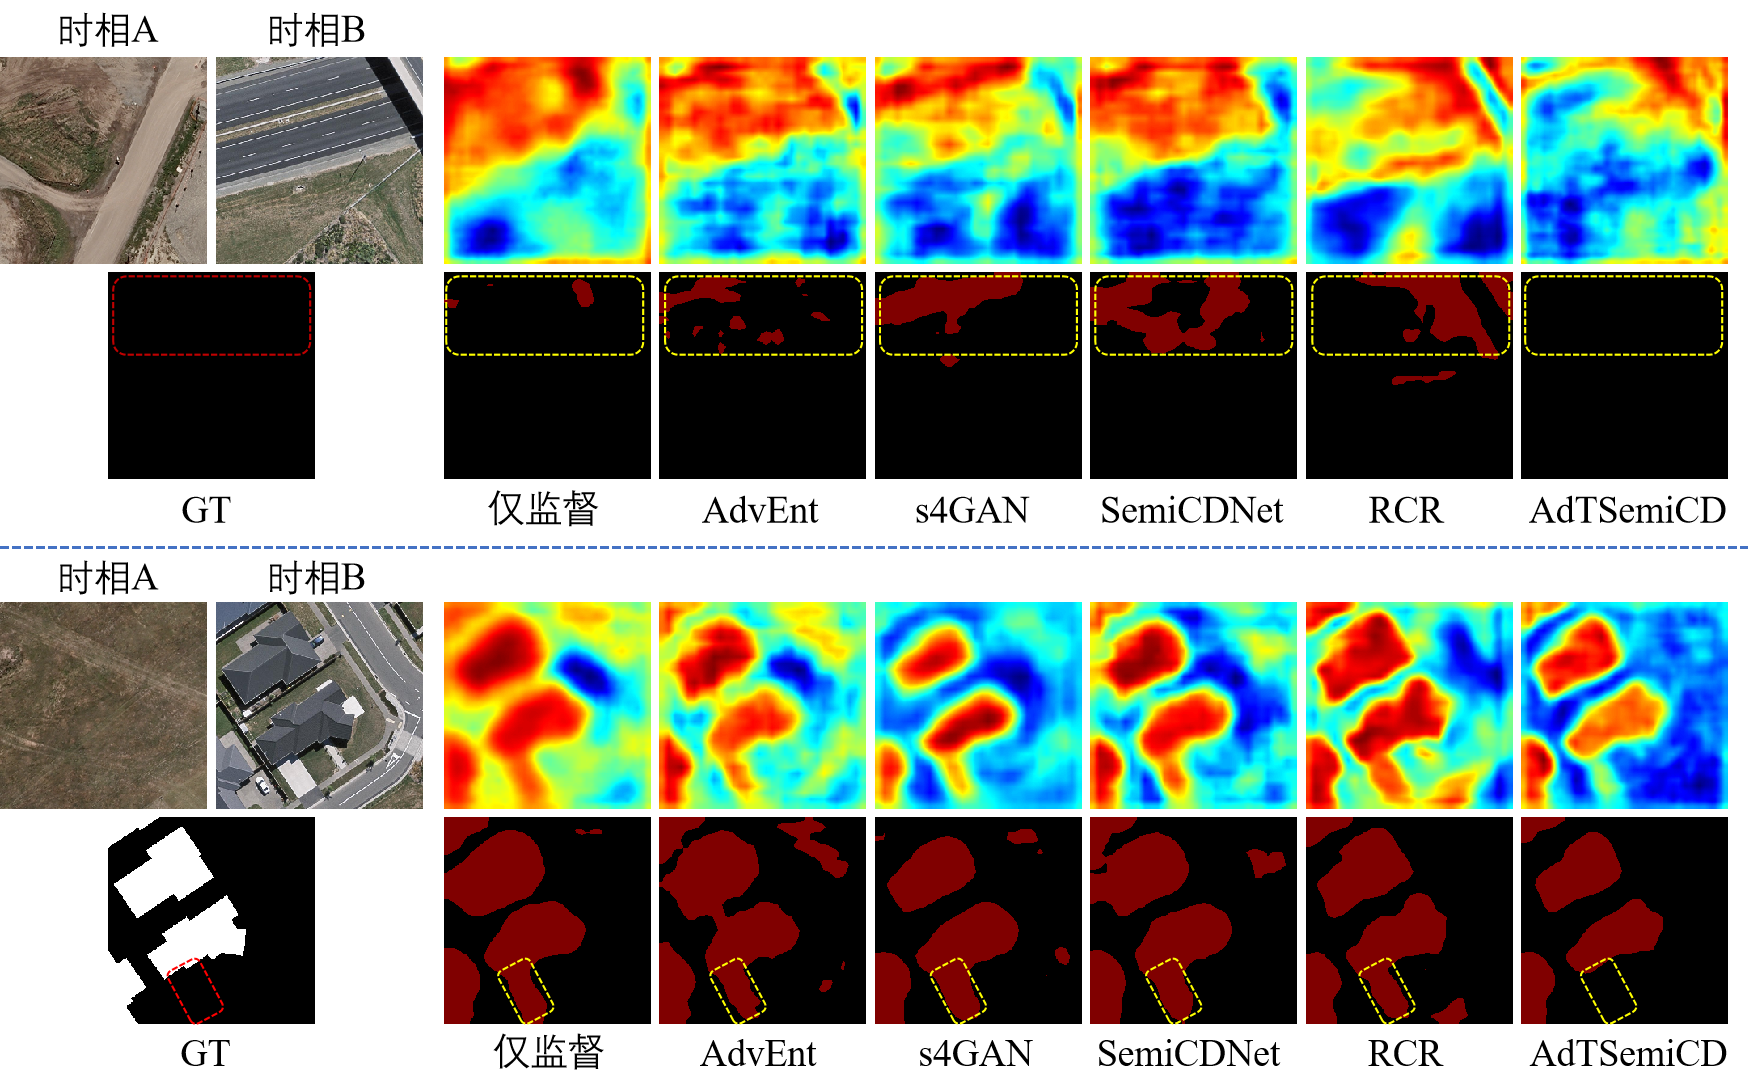
\includegraphics[scale=0.45]{images/AdTwhu-vis.png}
  \caption{
    5$\%$标记训练样本下AdTSemiCD与SOTA方法在WHU-CD测试集上的可视化对比图
  }
  \label{fig:AdTWhu-vis}
\end{figure}

显然在LEVIR-CD数据集上,我们的AdTSemiCD能够能够更好地识别边界,并且从热力图可以看出我们的方法在变化类别和不变类别上的预测置信度都比较高,区分度比较明显,这是因为我们提出的类别自适应阈值能够保证模型对两种类别的学习比较平衡并且充分学习到更多的上下文知识。在WHU-CD数据集上,我们的AdTSemiCD更好地排除了建筑物变化目标之外的干扰项,例如图\ref{fig:AdTWhu-vis}中的高速公路和水泥地,这些类型与建筑物比较相似,并且由于训练的标记样本稀少,进一步提高了准确识别建筑物变化检测的挑战性。AdTSemiCD更加充分地挖掘了样本中的隐藏信息,进而提升了在这些区域的识别能力。在CDD数据集上,本章方法的一个特点就是在细节上表现更佳,比如第一组可视化结果中草地间的土路。而CL-CD数据集上,所有方法比较容易出现的问题就是大面的错检、漏检,这对定量结果中$IoU$指标的影响比较剧烈,问题原因同样是标记样本的稀少,CL-CD数据集是十个数据集中数据规模最小的,在半监督设置下就更加稀少了。我们的方法在这些情况下表现良好,虽然边界识别可能并非完全准确,存在一些误差,但是总体上表现尚可,从热力图上可以看出,相比其他半监督方法,AdTSemiCD能够正确的判定出变化目标。
\begin{figure}[!htbp]
  \centering
  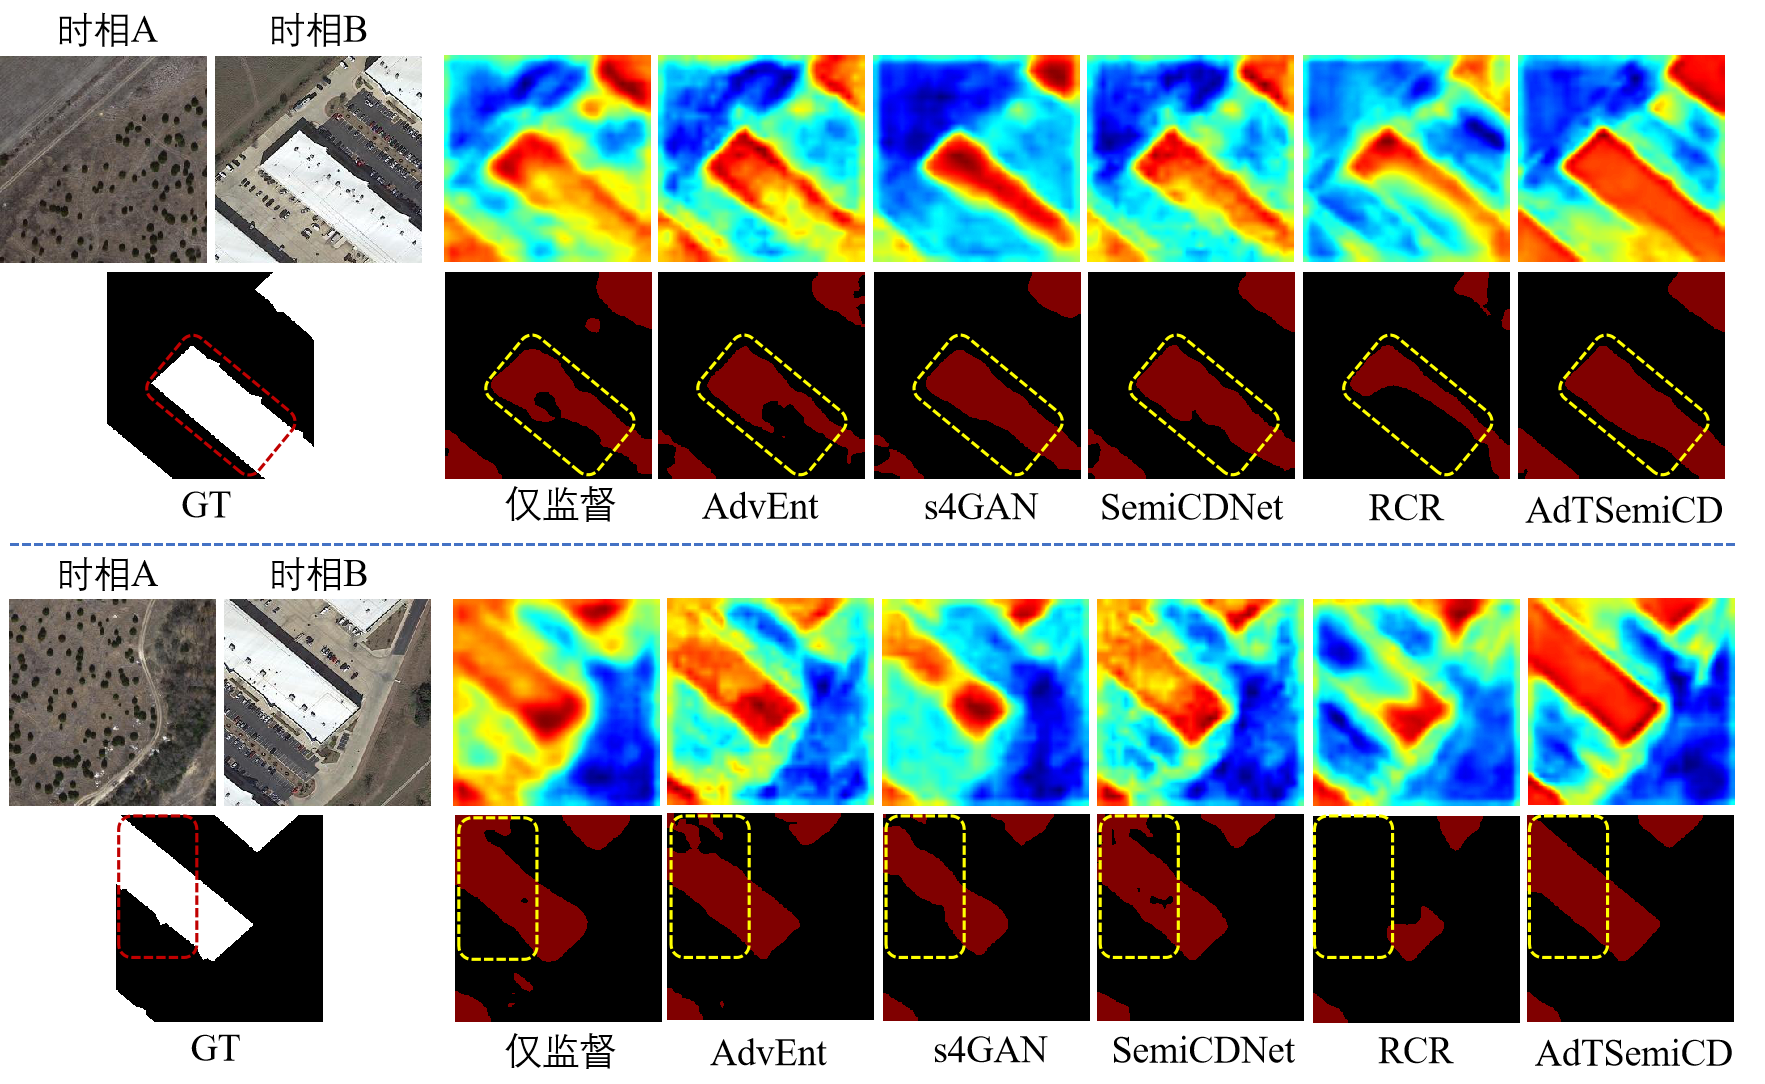
\includegraphics[scale=0.45]{images/AdTlevir-vis.png}
  \caption{
    5$\%$标记训练样本下AdTSemiCD与SOTA方法在LEVIR-CD测试集上的可视化对比图
  }
  \label{fig:AdTLevir-vis}
\end{figure}

图\ref{fig:AdTdiffLevir-vis}展示了不同标记率下训练的模型在相同测试样本上的变化检测可视化结果。可以看到随着标记训练样本的增多,模型的检测效果越好,尤其是在一些细节处的表现,并且我们的半监督变化检测算法仅在40$\%$甚至更少的标记需求下就取得了与Oracle相当的性能。
\begin{figure}[!htbp]
  \centering
  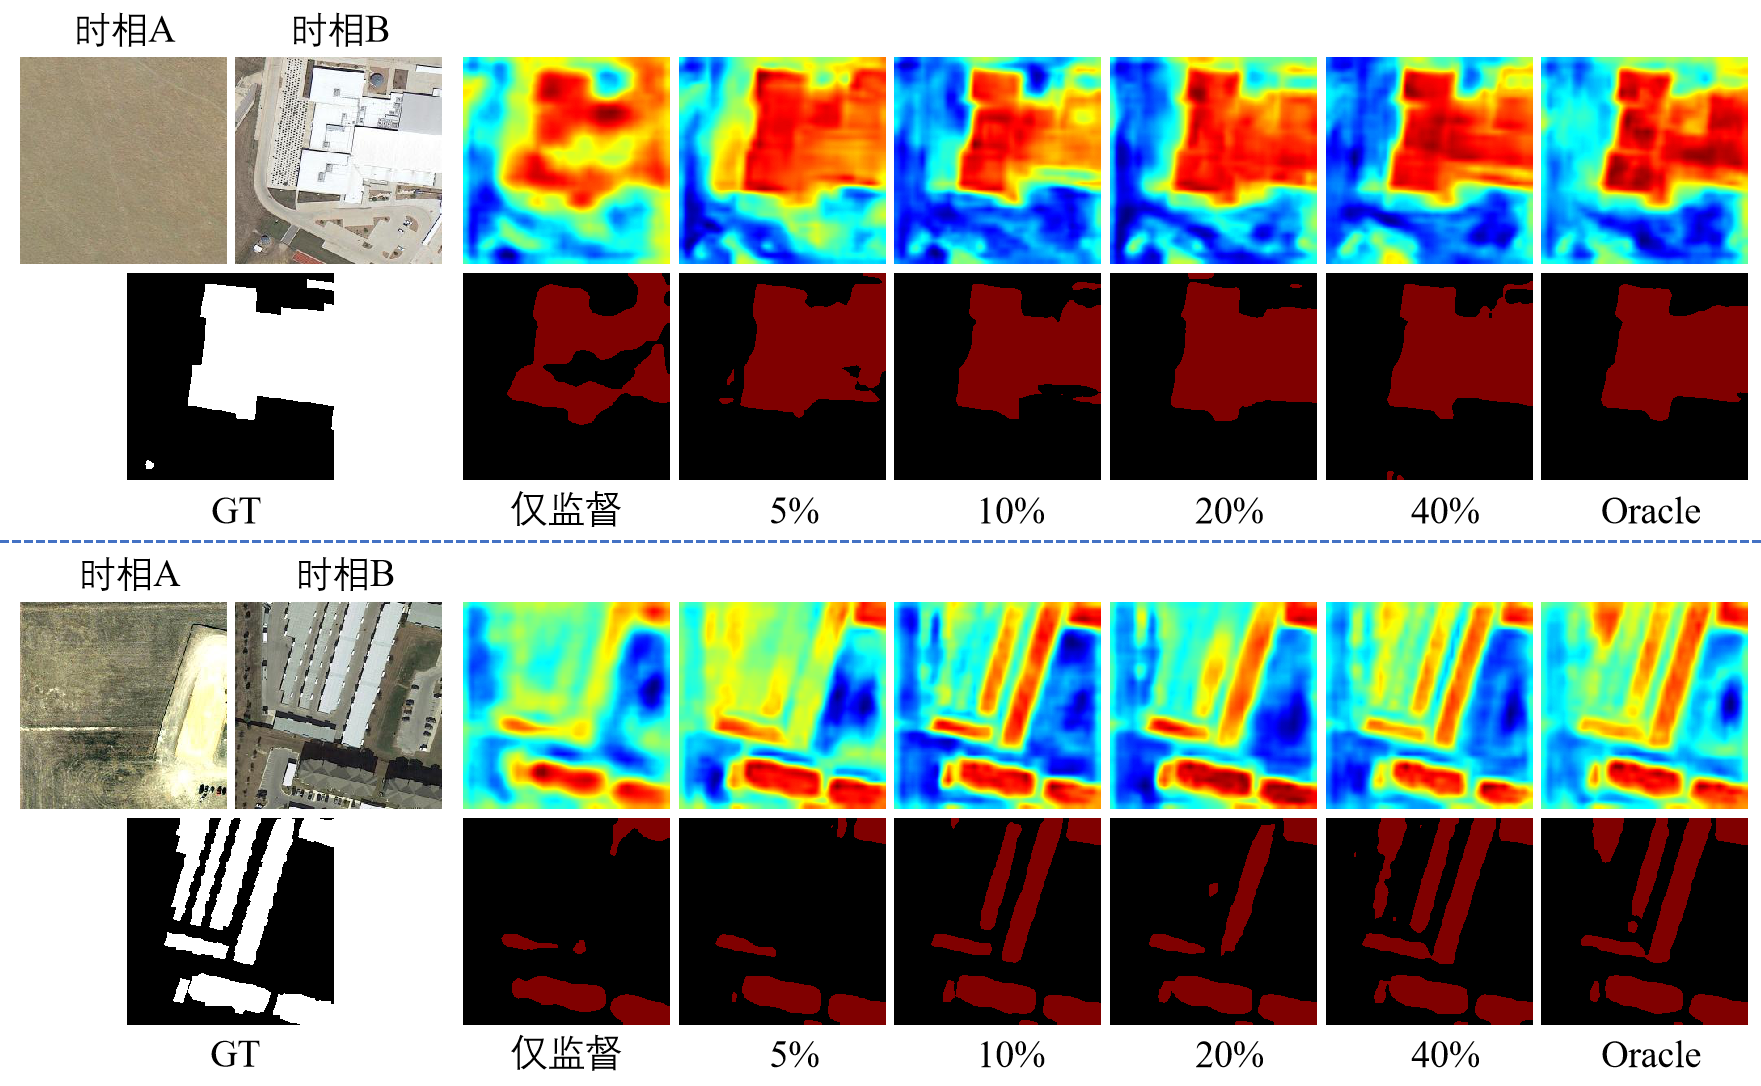
\includegraphics[scale=0.45]{images/AdTdiff_vis.png}
  \caption{
   不同标记率下AdTSemiCD在LEVIR-CD测试集上的可视化对比图
  }
  \label{fig:AdTdiffLevir-vis}
\end{figure}
除给出的可视化示例之外,在其余数据集以及其余样本上,我们的方法也表现出了与定性实验结果一致的优异性能。总而言之,自适应阈值使得我们的方法能够更加充分和平衡地学习到无标注样本的特征分布,低置信度学习进一步减小了错误伪标签带来的影响,因此在一些复杂区域、细节区域以及稀少样本类型上,我们的AdTSemiCD展现了其强大的判别能力。
\begin{figure}[!htbp]
  \centering
  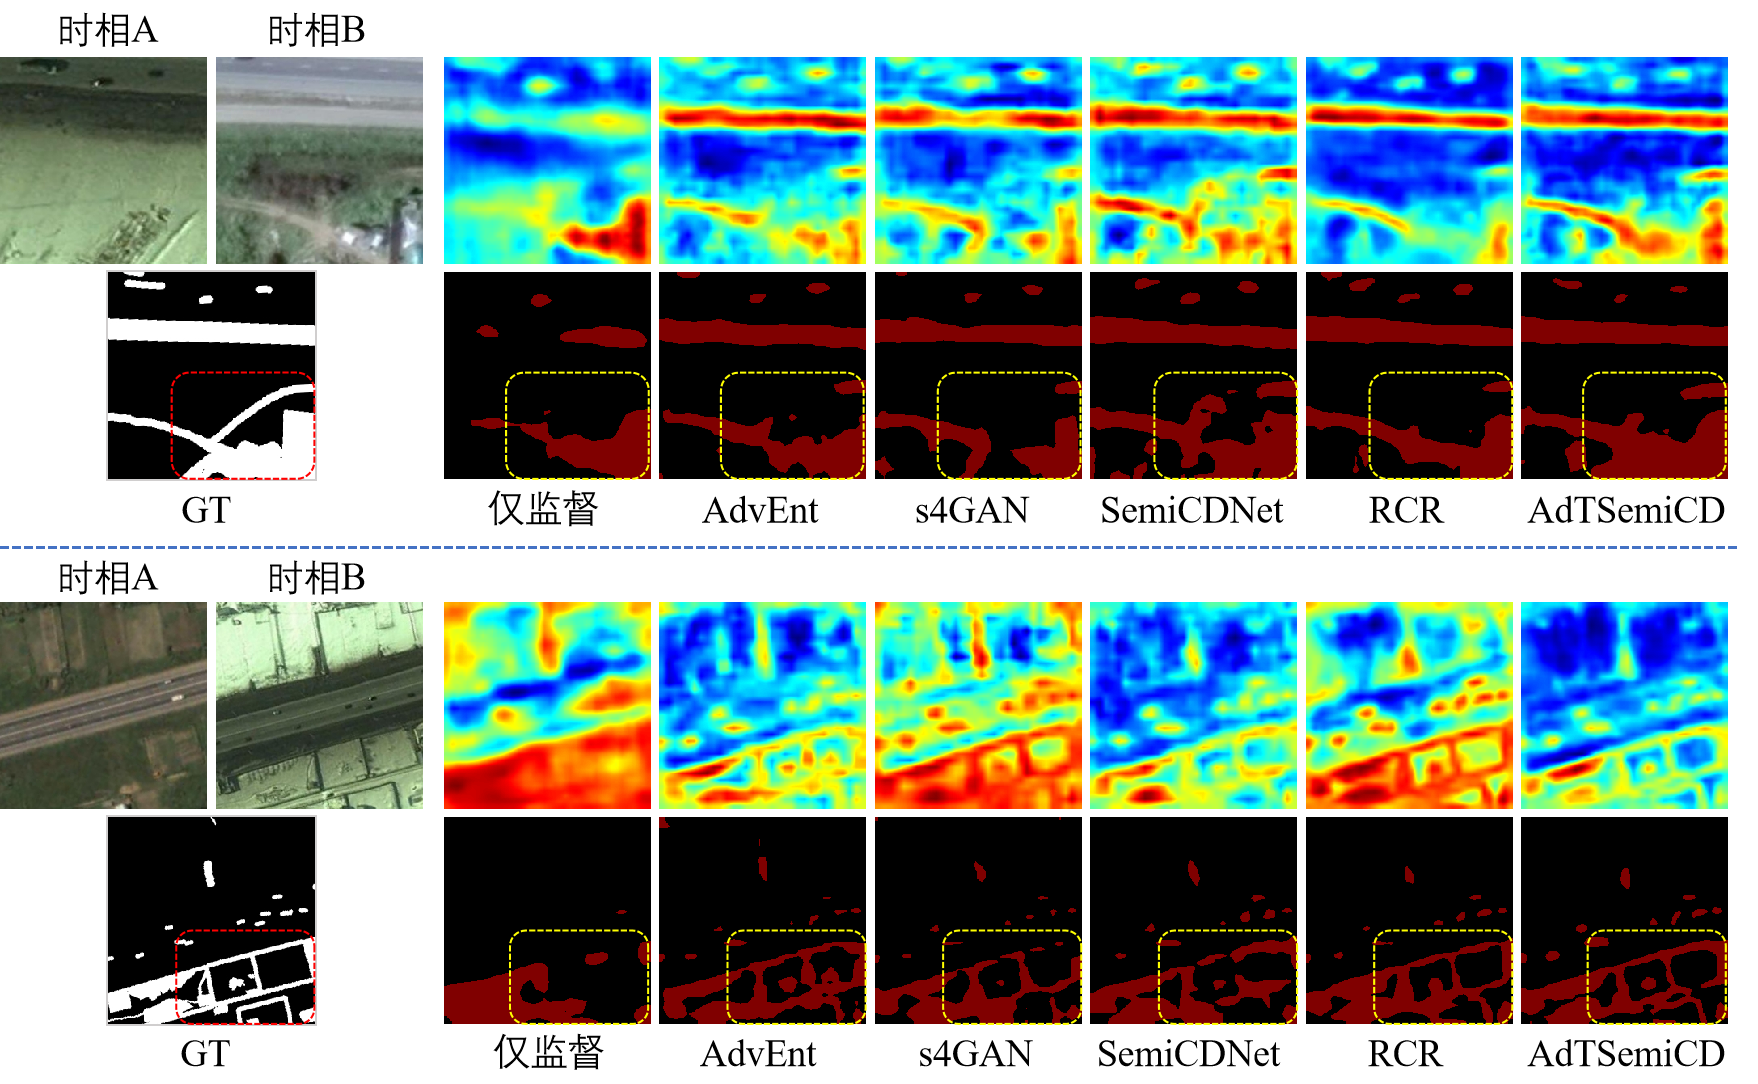
\includegraphics[scale=0.45]{images/AdTcdd-vis.png}
  \caption{
    5$\%$标记训练样本下AdTSemiCD与SOTA方法在CDD测试集上的可视化对比图
  }
  \label{fig:AdTCdd-vis}
\end{figure}
\begin{figure}[!htbp]
  \centering
  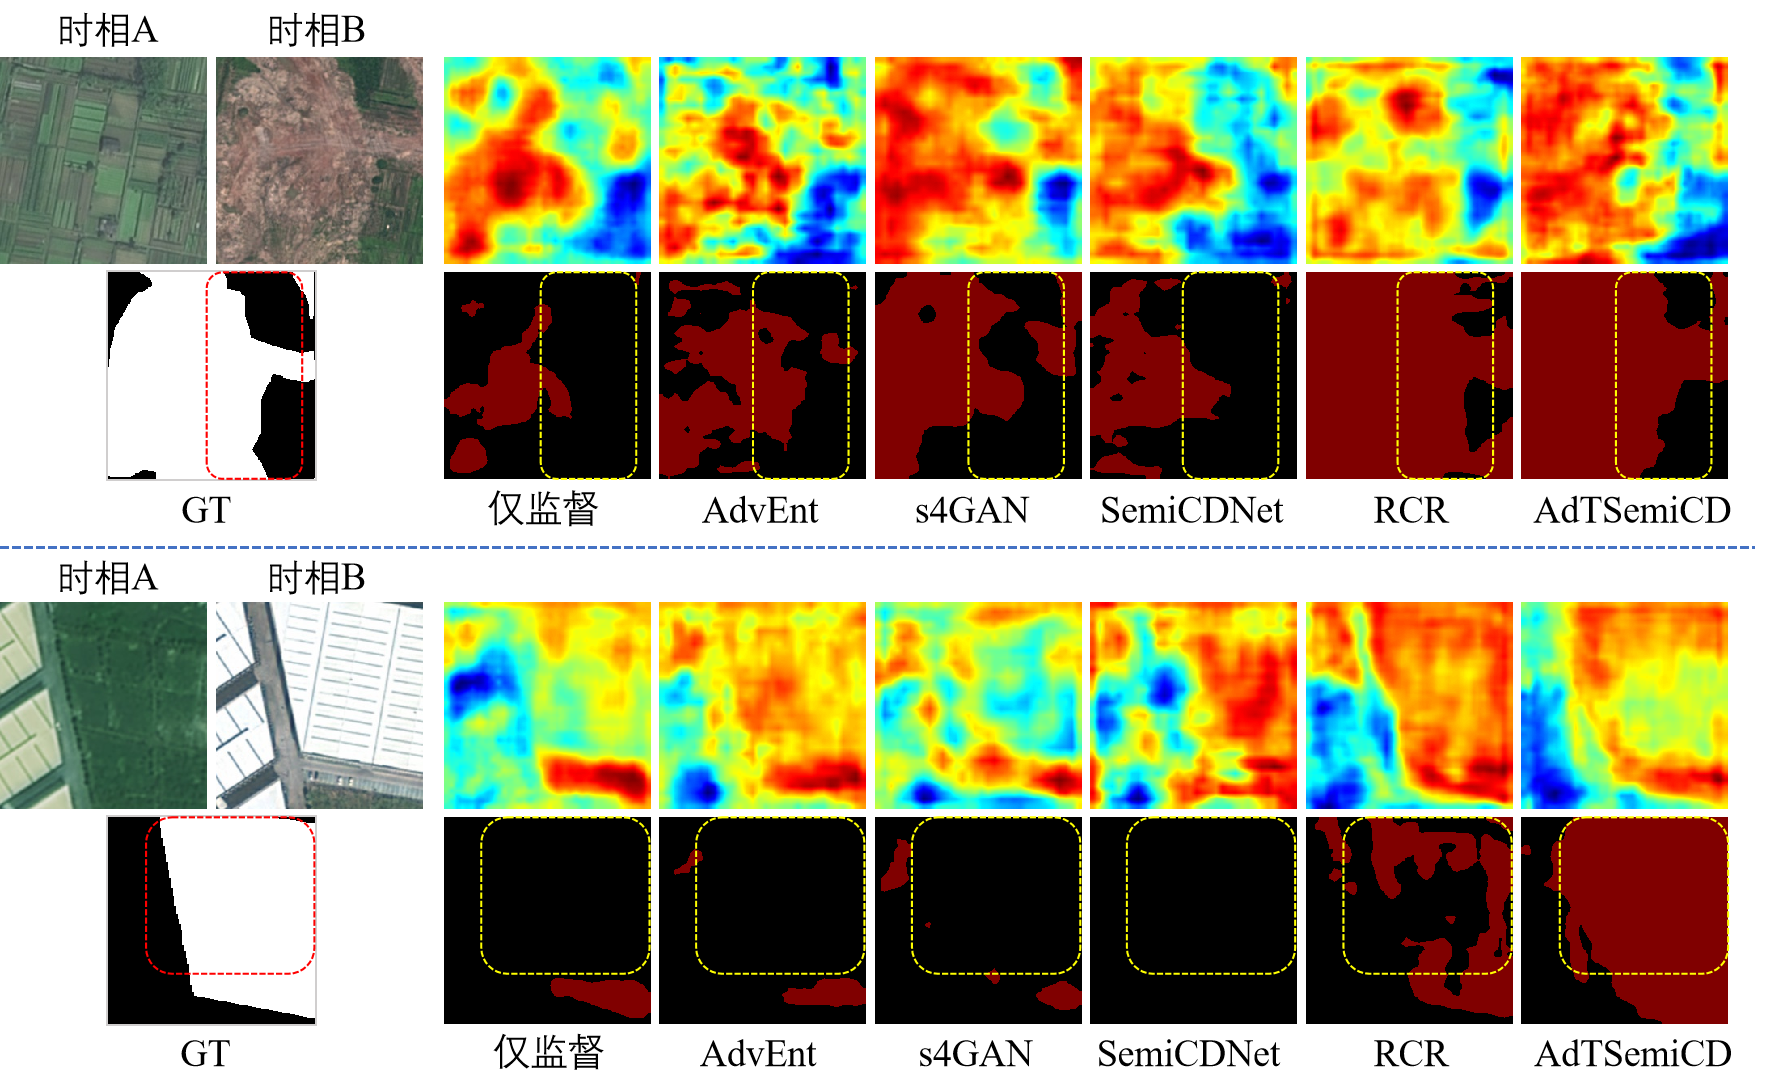
\includegraphics[scale=0.45]{images/AdTcl-vis.png}
  \caption{
    5$\%$标记训练样本下AdTSemiCD与SOTA方法在CL-CD测试集上的可视化对比图
  }
  \label{fig:AdTCl-vis}
\end{figure}
\subsection{消融实验}
\begin{table*}[!htbp]
  % \renewcommand\arraystretch{1.2}
\centering
% \tiny
\caption{在LEVIR-CD数据集上的自适应动态阈值消融研究}
   \resizebox{0.9\textwidth}{!}{
   % \setlength{\tabcolsep}{9pt}
\begin{tabular}{p{30mm}p{20mm}p{20mm}cp{20mm}p{20mm}cp{20mm}p{20mm}cp{20mm}p{20mm}} %
  \toprule
  \multirow{2}{*}{\parbox[c]{.2\linewidth}{Method}} & \multicolumn{2}{c}{5\%} & & \multicolumn{2}{c}{10\%} & & \multicolumn{2}{c}{20\%} & & \multicolumn{2}{c}{40\%}\\
  \cmidrule{2-3} \cmidrule{5-6} \cmidrule{8-9} \cmidrule{11-12}
  & {$IoU^c$} & {OA} && {$IoU^c$} & {OA} & & {$IoU^c$} & {OA} &&{$IoU^c$} & {OA}\\
  \midrule
  仅监督   &   61.0 & 97.60 && %5
                  66.8 & 98.13 && %10
                  72.3 & 98.44 && %20
                  74.9 & 98.60 \\ %40
    MT+NT      &   61.8 {\color{red} (+1.8)} & 98.66 {\color{red} (+0.06)} &&
                  67.9 {\color{red} (+1.1)} & 98.30 {\color{red} (+0.17)} &&
                  74.6 {\color{red} (+2.3)} & 98.59 {\color{red} (+0.15)}&&
                  76.4 {\color{red} (+1.5)} & 98.70 {\color{red} (+0.10)} \\
      MT+FT     &   67.1 {\color{red} (+6.1)} & 98.14 {\color{red}(+0.54)} &&
                  75.0 {\color{red} (+8.2)} & 98.63 {\color{red} (+0.50)} &&
                  76.6 {\color{red} (+4.3)} & 98.71 {\color{red} (+0.27)}&&
                  77.0 {\color{red} (+2.1)} & 98.73 {\color{red} (+0.13)} \\

      MT+AT &  69.9 {\color{red} (+8.9)} & 98.38 {\color{red} (+0.78)} && %5
                  75.3 {\color{red} (+8.5)} & 98.67 {\color{red} (+0.54)} && %10
                76.9 {\color{red} (+4.6)} & 98.74 {\color{red} (+0.30)} && %20
                  77.8 {\color{red} (+2.9)} & 98.79 {\color{red} (+0.19)} \\ %40
  \bottomrule
\end{tabular}
  }
% \normalsize
\label{tab:ablation_AdThresh}
\end{table*}
为了验证本章所提出的自适应动态阈值和低置信度学习的有效性,我们在LEVIR-CD数据集所有标记率下进行了消融实验,实验结果如表\ref{tab:ablation_AdThresh}和表\ref{tab:ablation_AdTModel}所示。其中,表中的缩写及其含义解释如下:

MT:Mean-Teacher,平均教师半监督学习框架。

NT:No Threshold,无阈值筛选,即将所有标签均视为可信标签。

FT:Fixed Threshold,固定阈值筛选,固定阈值设置为0.95。

AT:Adaptive Threshold,自适应阈值筛选。

LL:Low confidence Learning,低置信度学习。

在关于自适应动态阈值筛选的消融实验中,当对教师模型生成的伪标签不进行阈值筛选而直接指导学生模型训练时,相比基线,大量的无标记样本带来的提升却是微乎其微,这也说明了阈值筛选的重要性。使用0.95的固定高阈值能够带来巨大的改进,这是因为过滤掉了那些不可信的标签,仅使用高置信度的可靠伪标签指导模型的训练,这种自训练能够极大地扩充模型学习到的样本特征空间。最后,使用我们的基于模型学习状态的自适应动态阈值筛选机制,在固定阈值筛选的基础上进一步提升了模型的性能。得益于动态调整过程,模型在不同训练阶段使用了不同数量和质量的伪标签,不仅加快了模型的收敛速度,还提高了模型的泛化性。
\begin{table*}[!htbp]
  % \renewcommand\arraystretch{1.2}
\centering
% \tiny
\caption{AdTSemiCD在LEVIR-CD数据集上的消融实验}
   \resizebox{0.9\textwidth}{!}{
   % \setlength{\tabcolsep}{9pt}
\begin{tabular}{p{30mm}p{20mm}p{20mm}cp{20mm}p{20mm}cp{20mm}p{20mm}cp{20mm}p{20mm}} %
  \toprule
  \multirow{2}{*}{\parbox[c]{.2\linewidth}{Method}} & \multicolumn{2}{c}{5\%} & & \multicolumn{2}{c}{10\%} & & \multicolumn{2}{c}{20\%} & & \multicolumn{2}{c}{40\%}\\
  \cmidrule{2-3} \cmidrule{5-6} \cmidrule{8-9} \cmidrule{11-12}
  & {$IoU^c$} & {OA} && {$IoU^c$} & {OA} & & {$IoU^c$} & {OA} &&{$IoU^c$} & {OA}\\
  \midrule
  仅监督   &   61.0 & 97.60 && %5
                  66.8 & 98.13 && %10
                  72.3 & 98.44 && %20
                  74.9 & 98.60 \\ %40
  MT+FT      &   67.1 {\color{red} (+6.1)} & 98.14 {\color{red}           (+0.54)} &&
                  75.0 {\color{red} (+8.2)} & 98.63 {\color{red} (+0.50)} &&
                  76.6 {\color{red} (+4.3)} & 98.71 {\color{red} (+0.27)}&&
                  77.0 {\color{red} (+2.1)} & 98.73 {\color{red} (+0.13)} \\
  MT+AT     &   69.9 {\color{red} (+8.9)} & 98.38 {\color{red}           (+0.78)} && %5
                  75.5 {\color{red} (+8.7)} & 98.64 {\color{red} (+0.50)} && %10
                  76.8 {\color{red} (+4.5)} & 98.72 {\color{red} (+0.28)} && %20
                  77.7 {\color{red} (+2.8)} & 98.75 {\color{red} (+0.15)} \\ %40
  MT+FT+LL &  68.3 {\color{red} (+7.3)} & 98.21 {\color{red} (+0.61)} && %5
                  75.7 {\color{red} (+8.9)} & 98.64 {\color{red} (+0.51)} && %10
                77.0 {\color{red} (+4.7)} & 98.72 {\color{red} (+0.28)} && %20
                  77.3 {\color{red} (+2.4)} & 98.75 {\color{red} (+0.15)} \\ %40
  AdTSemiCD   &   71.3 {\color{red} (+10.3)} & 98.40 {\color{red} (+0.80)} &&
                  76.3 {\color{red} (+9.5)} & 98.66 {\color{red} (+0.53)} &&
                  77.2 {\color{red} (+4.9)} & 98.75 {\color{red} (+0.31)} &&
                  78.0 {\color{red} (+3.1)} & 98.79 {\color{red} (+0.19)} \\
  \bottomrule
\end{tabular}
  }
% \normalsize
\label{tab:ablation_AdTModel}
\end{table*}

在表\ref{tab:ablation_AdTModel}的AdTSemiCD的整体消融实验中,我们一方面在经典的平均教师半监督学习框架基线上,逐步替换和增加我们所设计的自适应动态阈值和低置信度学习模块,其中每个部分都取得了预期的提升效果,见表中第三行、第五行与仅监督基线的指标提升对比。另一方面,我们通过在两种不同的阈值方案上添加我们的低置信度学习模块,独立地证明了这一模块设计的有效性,见表中第二行与第四行以及表中第三行与第五行的指标提升对比,低置信模块分别在固定阈值筛选和自适应动态阈值筛选上取得了0.65和0.73个百分点的$IoU^c$提升,并且值得注意的是,低置信度学习在标记率越少的情况下效果越好,很显然这是因为标记数据越少,模型的预测更加不可信,因此那些被筛选掉的伪标签包含真实语义的概率也就越大,通过低置信度学习这种软伪标签可以将过滤掉的语义信息加以利用。
\begin{table*}[!htbp]
  % \renewcommand\arraystretch{1.2}
\centering
% \tiny
\caption{损失权重消融实验结果}
   \resizebox{0.9\textwidth}{!}{
   % \setlength{\tabcolsep}{9pt}
\begin{tabular}{p{10mm}p{20mm}p{5mm}cp{10mm}p{5mm}cp{10mm}p{5mm}cp{10mm}p{5mm}cp{10mm}p{5mm}} %
  \toprule
  \multirow{2}{*}{\parbox[c]{.1\linewidth}{$\lambda_{u}$}} & \multirow{2}{*}{$\lambda_{w}$} & \multicolumn{2}{c}{LEVIR-CD} & & \multicolumn{2}{c}{WHU-CD} & & \multicolumn{2}{c}{CDD} & & \multicolumn{2}{c}{CL-CD}\\
  \cmidrule{3-4} \cmidrule{6-7} \cmidrule{9-10} \cmidrule{12-13}
  && {$IoU^c$} & {OA} && {$IoU^c$} & {OA} & & {$IoU^c$} & {OA} && {$IoU^c$} & {OA}\\
  \midrule
  0  & 0 (Sup.Only) &   61.0 & 97.60 && %LEVIR-CD
                  50.0 & 97.48 && %WHU-CD
                  60.4 & 94.25 && %CDD
                  18.1 & 91.90 \\  %CL-CD
  0.5 & 0 &   68.1 & 98.20 && %5
                  62.9 & 98.17 && %WHU-CD
                  64.3 & 94.76 &&  %CDD
                  23.5 & 92.08 \\  %CL-CD
  1.0 & 0   &   69.9 & 98.38 && %LEVIR-CD
                  65.0 & 98.32 && %WHU-CD
                  65.7 & 94.96 &&  %CDD
                  25.9 & 92.14 \\  %CL-CD
  2.0 & 0   &   67.2 & 98.15 && %LEVIR-CD
                  63.8 & 98.24 && %WHU-CD
                  64.6 & 94.87 &&  %CDD
                  25.8 & 92.15 \\  %CL-CD
  1.0 & 0.5   &  70.6 & 98.35 && %LEVIR-CD
  \underline{\textbf{66.1}} & \underline{\textbf{98.41}} && %WHU-CD
                  67.9 & 95.37 &&  %CDD
                  27.6 & 91.90 \\  %CL-CD
  1.0 & 1.0   &   \underline{\textbf{71.3}} &         \underline{\textbf{98.40}} && %LEVIR-CD
                  66.0 & 98.41 && %10
                  \underline{\textbf{68.3}} & \underline{\textbf{95.52}} && %40
                  26.5 & 92.27 \\  %CL-CD
  1.0 & 2.0   &   71.0 & 98.39 && %LEVIR-CD
                  65.2 & 98.34 && %WHU-CD
                  67.7 & 95.42 &&  %CDD
                  \underline{\textbf{27.6}} & \underline{\textbf{92.32}} \\  %CL-CD
  \bottomrule
\end{tabular}
  }
% \normalsize
\label{tab:AdTPram_ablation}
\end{table*}

自适应动态阈值伪标签筛选的设计初衷在于提高无标记样本的利用率,因此我们进行了消融实验,在同样的半监督学习框架之上,以及固定阈值和自适应动态阈值两种方案下对无标记样本的利用率进行了对比,如图\ref{fig:AdT_util}所示,我们的自适应动态阈值筛选能够更大程度地挖掘无标记样本富含的信息,利用率从训练初期到训练完成均高于固定阈值筛选方法。此外还可以观察到的一点就是,在这种筛选机制下,能够更好地遏制由于少量标记样本造成的过拟合现象,在模型中后期仍然能够在无标记样本上生成可靠的伪标签。

此外,在总体损失公式\ref{eq:Adath_losstotal}中,无监督损失$\mathcal{L}_u$和低置信度学习损失$\mathcal{L}_KL$的权重分别为超参数$\lambda_u$和$\lambda_k$,我们对其取值进行了消融实验。表\ref{tab:AdTPram_ablation}展示了我们在四个数据集上以5$\%$标记率进行训练时的消融实验结果,其中在LEVIR-CD和CDD数据集上,当$\lambda_u$和$\lambda_k$分别取值为1.0、1.0时取得了最优结果;而在WHU-CD上,当$\lambda_u$和$\lambda_k$分别取值为1.0、0.5时取得了最优结果;以及在CL-CD上,当$\lambda_u$和$\lambda_k$分别取值为1.0、2.0时取得了最优结果。并且$\lambda_k$在CDD、CL-CD数据集上选择更加敏感。但整体都围绕(1.0,1.0)的参数组合上下略微波动,因此我们在其余数据集上均选择这两个数值作为两部分损失的权重。
\begin{figure}[!htbp]
  \centering
  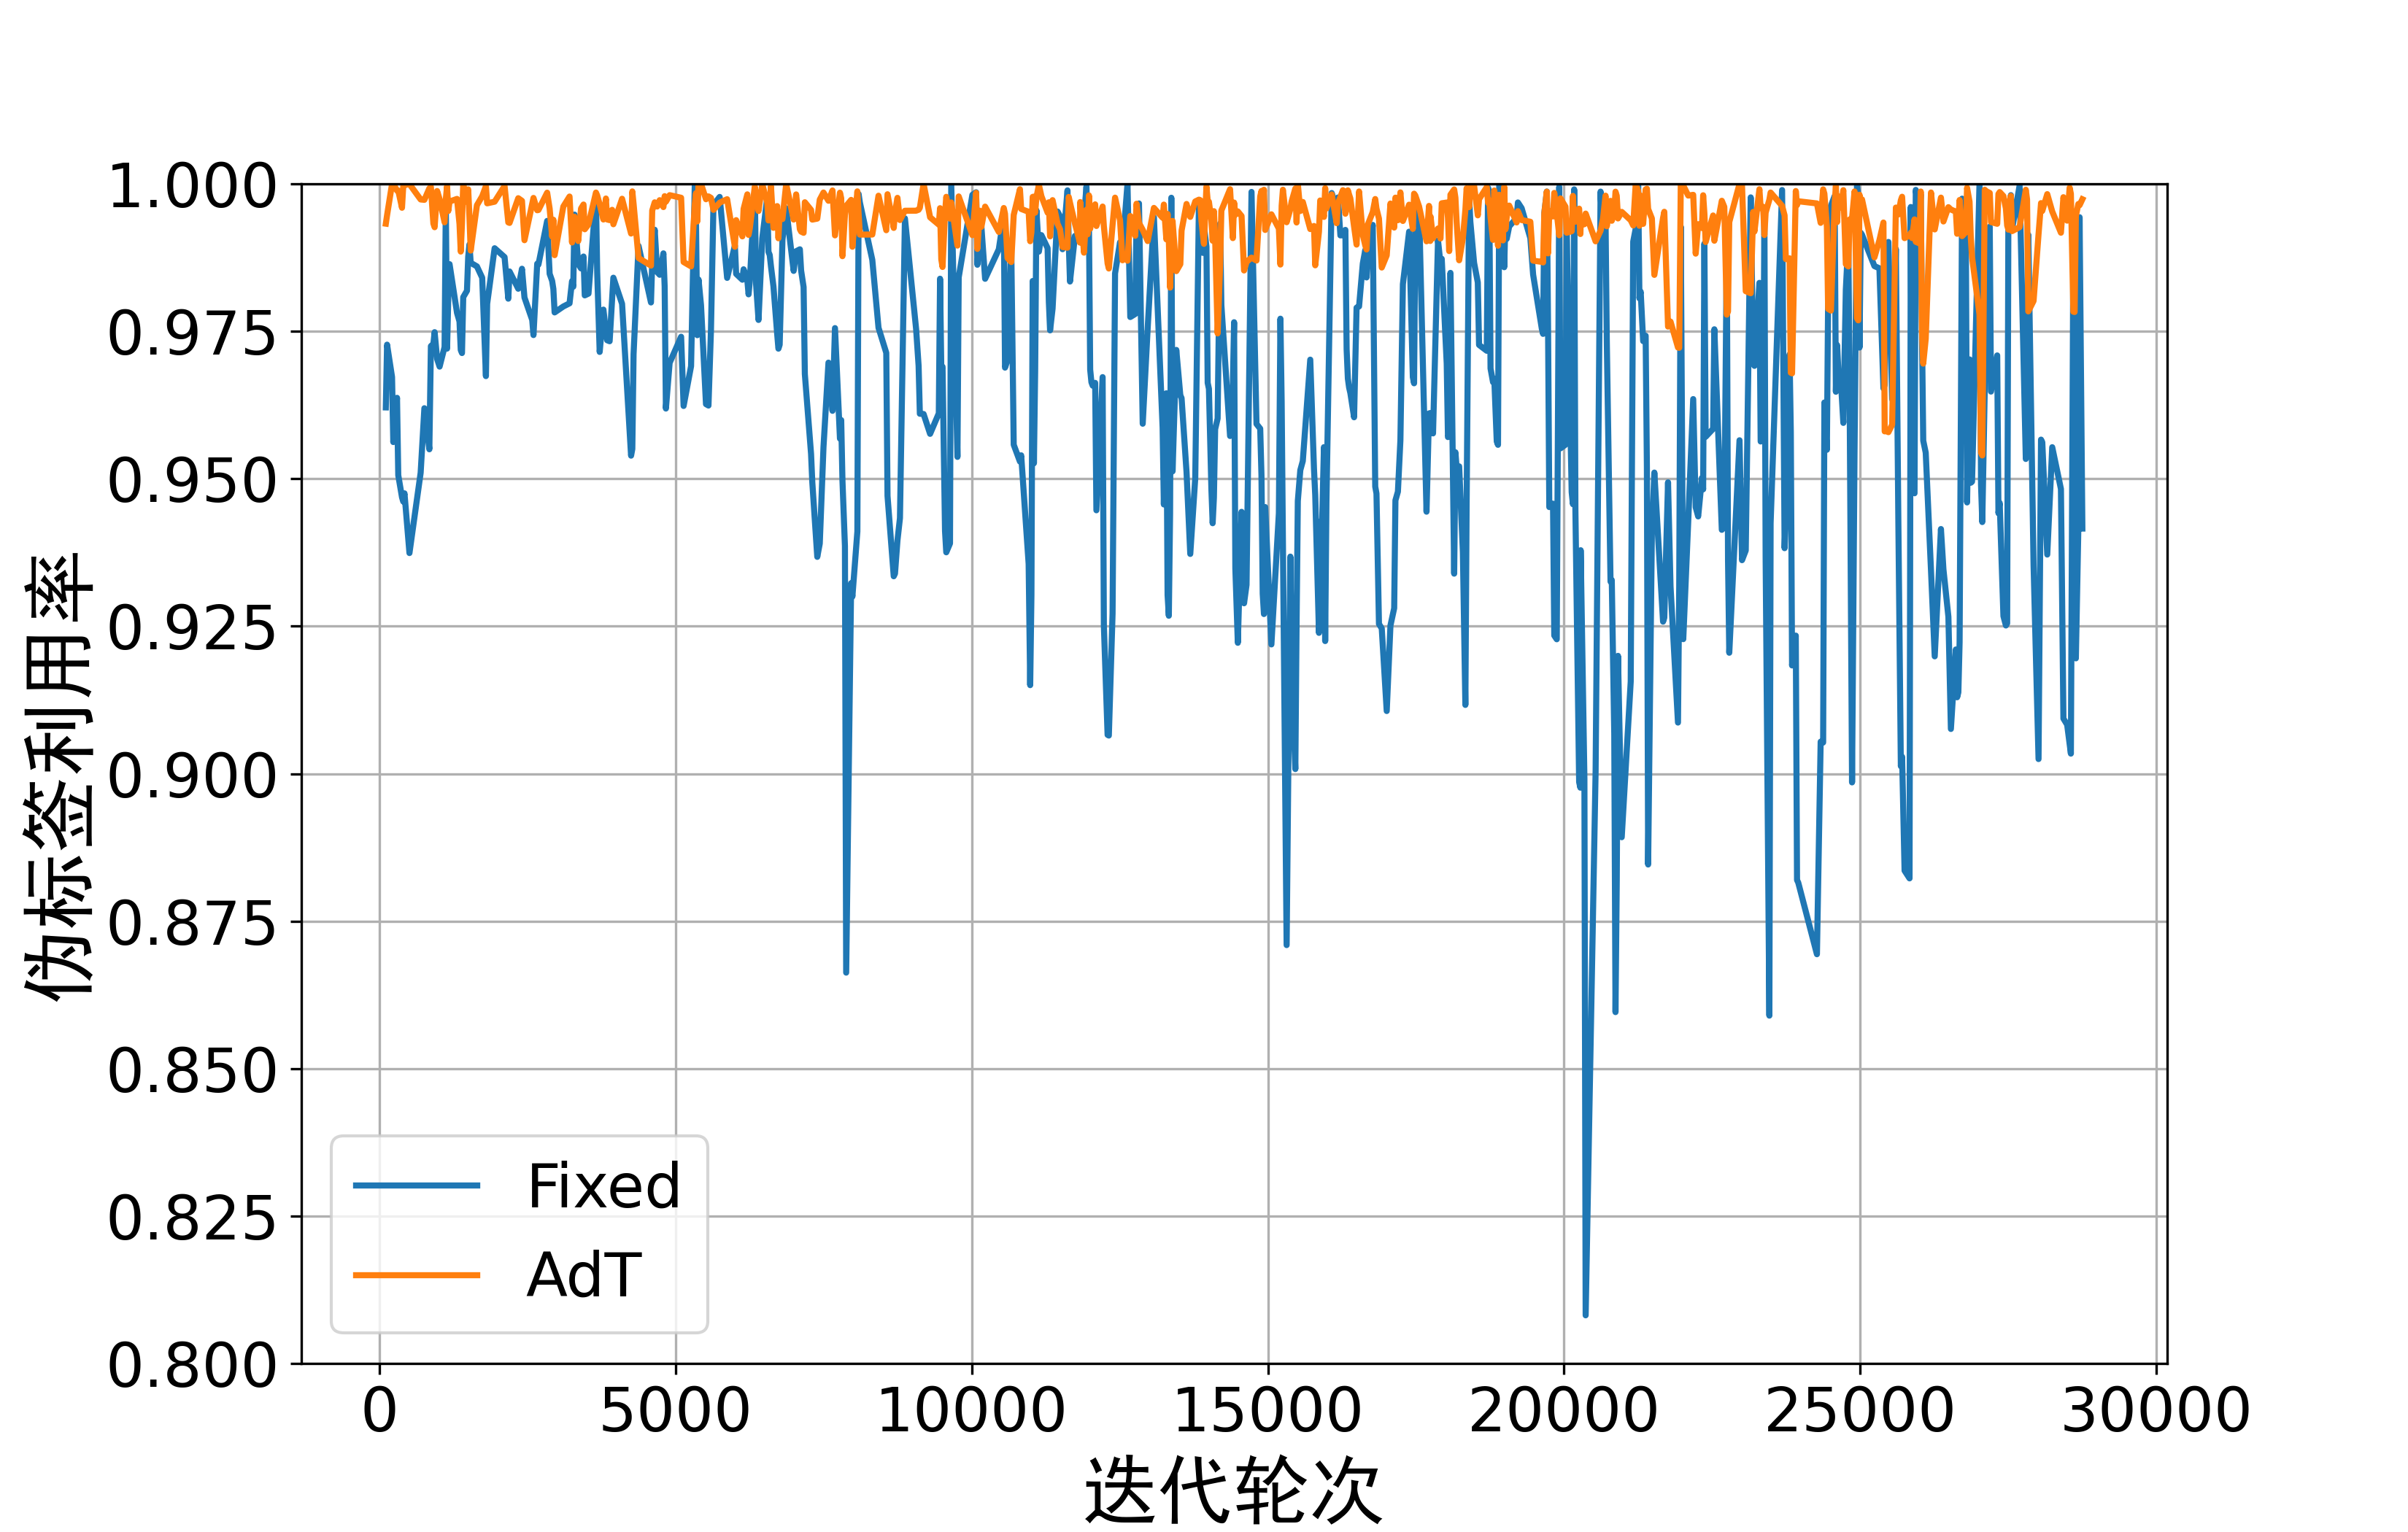
\includegraphics[scale=0.35]{images/AdTutil_ratio.png}
  \caption{
    训练过程中的伪标签利用率
  }
  \label{fig:AdT_util}
\end{figure}
\section{本章小结}
本章提出了基于自适应动态阈值的半监督变化检测算法,首先在引言部分分析了此前的阈值方法存在的局限性,针对模型对无标记样本学习不够充分的问题,提出了设计自适应阈值的必要性。之后详细介绍了本章的方法,从整体框架入手,再分别介绍了自适应动态阈值调整方法和低置信度学习模块。最后在所有十个数据集上进行了实验验证,从定性和定量两个角度验证了本章方法与其他几种对比半监督方法的性能,以及进行了消融实验证明本章方法中每个部分设计的合理性和有效性。
\cleardoublepage
\chapter{基于伪标签评估的自适应半监督变化检测算法}
\section{引言}
变化检测是遥感的一个重要领域,其主要重点是确定卫星在同一区域以不同间隔拍摄的双时相图像对中的变化区域。考虑到为变化检测任务准确标注掩码的过程是劳动密集型的,半监督变化检测是更有前景的方法。半监督变化检测的范式通常是通过利用有限的可用标签和大量未标记的样本来提高变化检测性能。对未标记的数据生成伪标签,这些伪标签通常是具有较高预测概率的临时预测掩码,将其作为训练过程中的指导信号,通过混合训练具有实际标签的有限数据和具有伪标签的丰富数据,学生模型可以学习到更多重要的特征,从而显著提高性能。最流行的方法是平均教师\cite{Tarvainen2017teacher}框架,它使用一个教师模型来生成伪标签,在训练过程中为学生模型提供指导。随后使用学生模型的指数移动平均(EMA)更新教师模型。

虽然这些方法已经获得了一定的成功,但仍然存在重大问题:即模型以同样的方式处理所有样本,而不考虑不同样本之间必然存在的差异性,并且训练过程缺乏灵活性。首先,很明显,未标记的样本可能并不总是能够胜任“教师”角色。模型在为复杂的样本生成可靠的高质量伪标签时经常遇到困难,这反过来又引入了额外的噪声,可能会误导模型的训练。

此外,EMA更新过程也没有考虑这种噪声干扰。考虑到训练批次中可能存在偏差或包含噪声,动态确定训练更新有助于训练过程的稳定性。这些因素强调需要更精确的监督方法,否则可能会对模型的训练产生负面影响。在本研究中,我们引入了一种自适应动态学习策略AdaSemiCD,旨在提高伪标签的准确性并简化训练过程。我们的框架结合了传统的半监督训练方法,并辅以两个创新的功能模块AdaFusion和AdaEMA。首先,我们利用AdaFusion在单个样本水平上抑制噪声,从而提高伪标签的准确性。与之前依赖于完全随机融合区域的Augseg\cite{AugSeg}或CutMix\cite{yun2019cutmix}等方法相反,我们的AdaFusion模块主动识别可能最不确定的区域,并将其替换为来自高质量标记数据集或未标记数据集的可靠内容。在此之后,我们通过AdaEMA模块动态调整师生模型的参数更新选择批次,以确保提高稳定性。虽然传统的EMA有效地减轻了模型参数的波动从而提高了稳定性,但它在每次训练迭代后都统一的更新参数,在处理一系列训练样本时忽略了模型在不同迭代中的不同学习效果。如果未标记的样本包含大量错误信息,它可能会误导模型的训练。因此,我们的AdaEMA引入了模型级参数更新的自适应选择过程,使模型能够充分集成优越的参数。

本章阐述了基于伪标签评估的自适应半监督变化检测算法——AdaSemiCD,首先介绍了模型的整体框架以及训练流程,随后详细介绍了设计的伪标签评估指标,以及基于此指标设计的两个自适应模块。最后在实验部分报告了该研究方法在十个公开数据集上取得的实验结果,并与其他经典半监督变化检测算法在定性和定量两个维度进行了公平的对比,证明了我们的方法优越性。最后通过消融实验证明了每个模块的有效性。
\section{基于伪标签评估的自适应半监督变化检测框架}
\subsection{整体框架}
AdaSemiCD的整体框架如图\ref{fig:Ada_fram}所示,与第三章AdTSemiCD类似,也才应平均教师模型作为主体框架。不同之处在于,AdaSemiCD基于教师模型对无标记样本的输出结果,在无标记样本对上进行了进一步的样本融合操作,以及在教师模型权重更新时采用了AdaEMA方式。
\begin{figure}[!htbp]
  \centering
  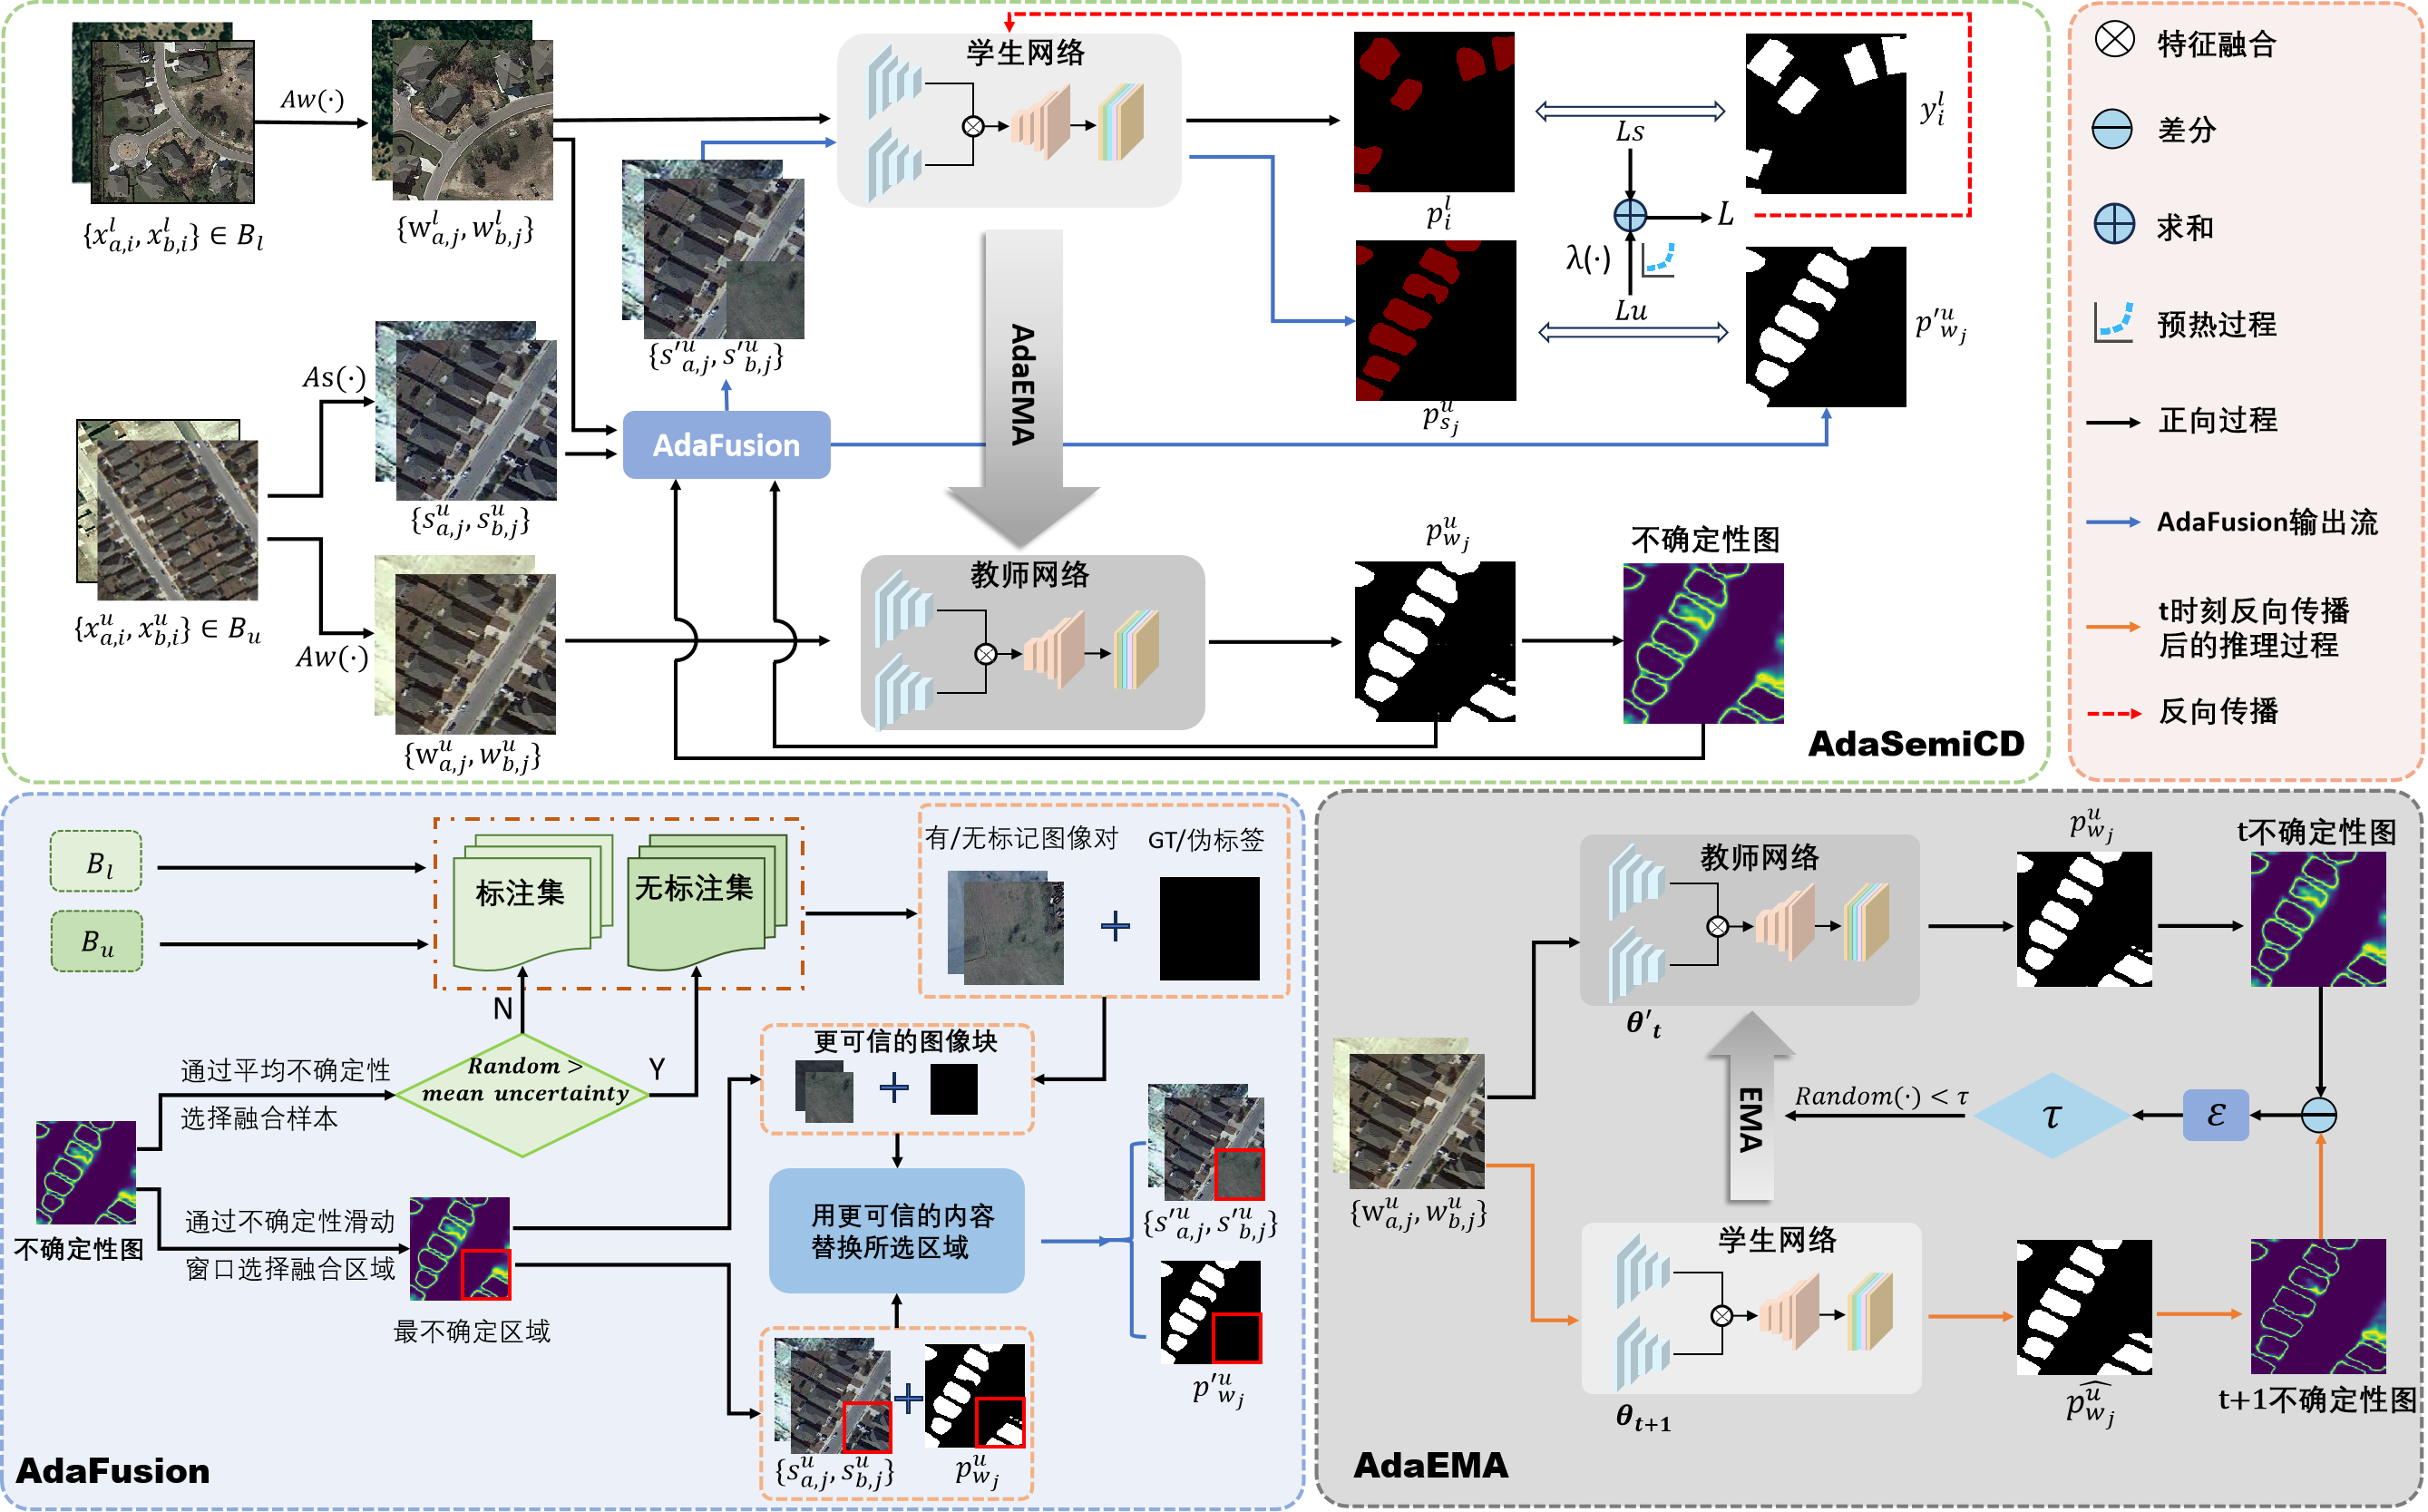
\includegraphics[scale=0.35]{images/AdaFrame.png}
  \caption{
    AdasemiCD的整体框架图
  }
  \label{fig:Ada_fram}
\end{figure}

此外,在初始训练阶段,我们的模型对未标记的样本生成的伪标签是高度不可靠的;在这个阶段过度依赖无监督训练可能会引入严重的噪声。相反,随着训练进入中后期阶段,模型越来越多地从有限的标记数据中学习,伪标签的质量得到提高,这时减少监督训练相对于非监督训练的比例是合理的。为了减轻过拟合现象和增强特征空间,必须实现一个受控过程来动态调整这两个分量在损失函数中的贡献。因此,在AdaSemiCD中我们使用一个预热过程来控制未标记部分的训练速度。$\lambda(\cdot)$为无监督损失随训练步长变化的权值,用于动态调整不同阶段有监督和无监督训练的比例,表达式如\ref{eq:ramp-up}所示。
\begin{equation}
  \label{eq:ramp-up}
  \lambda(\cdot)=w_{\max } \times e^{-\phi \times\left(1-\text { iter }_{\text {cur }} / \text { iter }_{\max }\right)^{2}},
\end{equation}
\begin{equation}
  \label{eq:ramp-upIter}
  { iter }_{\max }=\gamma \times { iter }_{sum }
\end{equation}
其中$w_{\max }$和$\phi$是超参数,$w_{\max }$表示无监督损失的最大可达权重,$\phi$用于控制上升的剧烈程度;$\text { iter }_{\text {cur }}$表示当前迭代周期;$\text { iter }_{\text {max }}$为预热过程的总步长,由\ref{eq:ramp-upIter}计算得到,${ iter }_{sum }$为整个训练过程的总迭代次数,且$0<\gamma<1.0$;在上升过程之后,无监督损失的权重保持为$w_{\max }$不变。在训练的早期,该权值相对较低,无监督训练的作用可以忽略不计,但在训练的中后期,该权值逐渐增大,加权后的无监督损失超过了有监督损失,因此无监督训练占主导。

\textbf{自适应模块}:半监督学习的本质在于伪标签的质量。然而,很明显,前面提到的过程没有考虑到不同样本个体对模型训练的不同影响。本章研究主要关注与伪标签生成直接相关的两个元素:未标记图像对,以及伪标签生成网络(即教师模型)在识别变化方面的性能。为了给未标记信息提供更可靠的监督指导,减少训练的不确定性,我们设计了一种自适应训练策略来解决这两个关键问题。我们首先设计了一个度量标准,用于量化伪标签的不确定性,作为自适应调整的基础。接下来,我们提出图像层面对未标记的训练样本进行自适应改造。此外,还提出在训练阶段对教师网络应用自适应选择性的EMA更新,以集成更加正确的参数,从而产生更一致和更高质量的伪标签。这些努力将在下面的小节中进行详细阐述。
\subsection{伪标签评估指标设计}
为了通过准确测量伪标签的质量来提高其有效性,关键的一步就是评估指标的设计。这个度量将有助于识别可靠的标签和确定每个训练样本的效力。与带有标记图像对的场景不同,可以将真实标签作为基准,通过预测与真是标签的平均交并比、F1分数等来评估模型的推理质量,而伪标签缺乏任何这样的参考,其只能与自己进行比较。

因此,我们专门为伪标签设计了一个可量化的评估指标,旨在总体信息熵的基础之上,同时考虑到类别不平衡和混淆区域等因素。信息熵是一种衡量模型性能的常用指标,计算公式如下:
\begin{equation}
  \label{eq:entropy}
  E\left(x_{i}\right)=-P\left(x_{i}\right) \log _{2} P\left(x_{i}\right)
\end{equation}

其中$P\left(x_{i}\right)$为模型对于样本$x_{i}$的输出概率。我们认为,预测值中的信息熵越低,预测结果的可信度越高。相反,信息熵越高,预测结果的变化越大,同一像素上的预测概率分布越均匀,类别之间的差异越小。

在变化检测任务中,由于类别不平衡带来的巨大挑战,直接应用信息熵通常不会产生良好的结果。如图\ref{fig:Adasemicd_imbalance}所示,我们在10个公开的变化检测数据集上进行了统计分析,变化和不变类别的比例是极度失衡的。这种类别不平衡现象会导致模型在训练过程中学习目标类别不够充分,而过度地拟合不变类别的特征分布。因此,在推理过程中,模型更倾向于将像素分类为背景类。因此,尽管该模型的总体精度(OA)看起来很高,但在目标类别的交并比($IoU^c$)上的性能仍然令人不满意。为了在评估伪标签质量时最大限度地减少这种类别不平衡的影响,我们在计算信息熵时为两个类别分配了不同的权重,如\autoref{eq:balance}所示。
\begin{equation}
  \label{eq:balance}
  E^{\prime}(x_i)=w_{1} \times E\left(x_{i}\right)[0]+w_{0} \times E\left(x_{i}\right)[1]
\end{equation}

其中$w_{0}$和$w_{0}$分别表示当前小批次中属于不变类和变化类别的像素的比例。其计算公式如\autoref{eq:w0}和\autoref{eq:w1}所示。
\begin{equation}
  \label{eq:w0}
  w_{0}=\frac{\sum_{i=1}^{|B u|} \sum_{k=1}^{H \times W}\left(P\left(x_{i}\right)==0\right)}{|B u| \times H \times W},
\end{equation}
\begin{equation}
  \label{eq:w1}
  w_{1}=\frac{\sum_{i=0}^{|B u|} \sum_{k=0}^{H \times W}\left(P\left(x_{i}\right)==0\right)}{|B u| \times H \times W}
\end{equation}

此外,来自边界、目标与背景相似的区域的像素,模型的预测通常具有很大的不确定性,应该得到更多的重视。首先,我们通过计算两类预测概率之差的绝对值来增强这些易混区域的影响:
\begin{equation}
  \label{eq:abs}
  D\left(x_{i}\right)=\operatorname{abs}\left(P\left(x_{i}\right)[1]-P\left(x_{i}\right)[0]\right)
\end{equation}

这里,$\operatorname{abs}$表示取绝对值运算,这是一种用来防止前后时相变化检测不幂问题的措施。然后利用信息熵进行逐像素相乘运算,最终得到图像的不确定性映射图$U\left(x_{i}\right)$:
\begin{equation}
  \label{eq:uncertainty}
  U\left(x_{i}\right)=1-D\left(x_{i}\right) \cdot E^{\prime}\left(x_{i}\right)
\end{equation}

显然,在低信息熵的像素位置,该过程不会导致显著的变化,而在高信息熵的像素位置,其值将显著减小,直接使用该指标与所表达的意义相反。因此,我们采用校正信息熵的逆作为其描述。

综上所述,为了评估变化检测伪标签的质量,我们提出了一个可量化的计算度量$U$来衡量预测不确定性,该度量考虑了类别不平衡等因素并增加了对混淆区域的关注,从而在总体信息熵的基础上表达了更多有价值的信息。
\subsection{自适应样本融合机制}
图像融合经常被用来增强或者改造训练样本以提高样本多样性,CutMix\cite{yun2019cutmix}和MixUp\cite{zhang2017mixup}是典型的融合方法。在本研究中,我们的目标是利用图像融合技术来排除训练样本中的不可靠区域。这个过程包括两个步骤:1)融合区域选择;2)融合图像选择。

\textbf{融合区域的自适应选择}。与传统的随机选择混合区域的CutMix技术不同,我们的方法更加精细。首先我们将初始化一个随机大小的边界框,然后沿着图像坐标滑动窗口,维护一个总体最大不确定性框,最终选择总体不确定性最高的区域作为融合区域。

这些区域通常是边界或复杂的区域,模型在这些区域的检测性能受限,很难准确识别变化目标,因此如果不做处理地直接用于训练,就会引入大量的噪声干扰,这对模型训练有很大的影响。

\textbf{融合内容的自适应选择}。对于最大不确定性的区域,我们可以选择从样本集中选择一个其余更可信的样本替代这部分,可选样本来自标记数据集$B_l$或y有着更高可靠性的未标记数据集$B_u$。这种策略可以防止过度使用仅有的少量标记样本,进一步降低过拟合的风险。这里融合内容使用图像块而不使用实例对象,这是因为我们认为过多的人为干预可能会破坏模型的泛化能力,并且仅替换实例对象可能造成周围像素的失真。

融合内容的选择主要通过自适应调整决策上界来确定融合内容。我们直接使用同一个小批次内计算的不确定性均值作为决策上界,对每个小批次随机生成一个概率值(0到1之间),如果超过不确定性均值,代表当前样本包含的噪声过多,则随机从标记图像批次中选择一对图像作为融合内容。我们会维护根据不确定性排序维护一个批次不确定性队列集合,如果小于此上界,则从此队列集合中均匀选择TopK的未标记的图像对。很容易理解,无标注样本的伪标签质量越高。可以被认为足够可靠。而不确定性越高的样本噪声越大,融合标记样本可以显著降低噪声密度,融合过程如图\ref{fig:Adasemicd_fram}左下角的AdaFusion子图。
\begin{algorithm}[!htbp]
  \caption{AdaEMA算法}
  \label{alg:AdaEMA}
  \begin{algorithmic}[1] % 这个1 表示每一行都显示数字
  \Require ~~\\
    学生模型$M_{stu}^{\theta}$,教师模型$M_{tea}^{\theta}$ \\
    当前批次的训练样本集$\mathcal{B} = \left \{\mathcal{B}_l, \mathcal{B}_u\right \}$
  \Ensure ~~\\
    更新后的教师模型$M_{tea}^{\theta'}$ \\
  \State 在标记样本$\mathcal{B}_l$上根据\ref{eq:AdaLossS}计算监督损失$\mathcal{L}_{s}$;
  \State 在无标记样本$\mathcal{B}_u$上根据\ref{eq:AdaLossU}计算无监督损失$\mathcal{L}_{u}$;
  \State 根据SGD最小化总训练损失来更新学生网络参数$M_{stu}^{\theta}$为$M_{stu}^{\theta'}$;
  \State 根据\ref{eq:uncertainty}计算教师模型在无标记样本上生成的伪标签的不确定性${U}_{tea}$;
  \State 根据\ref{eq:uncertainty}计算更新后的学生模型在无标记样本上的预测结果的不确定性${U}_{stu}$;
  \State 根据公式\ref{eq:varepsilon}和\ref{eq:tau}计算教师模型此次迭代更新概率的上界$\tau$;
  \If{$random(\cdot)<\tau$}
    \State 根据指数移动平均公式\ref{eq:ema}更新教师模型参数为$M_{tea}^{\theta'}$;
  \Else
    \State $M_{tea}^{\theta'} = M_{tea}$;
  \EndIf
  \State \textbf{Return:} $M_{tea}^{\theta'}$;
  \end{algorithmic}
\end{algorithm}
\subsection{自适应师生模型参数更新机制}
在平均教师框架中,通过对学生模型参数在时间序列上的移动指数平均得到教师模型的参数,这种方法与共享权重的孪生网络相比,更加稳定可靠。然而,我们对平均教师模型的期望是达到共同进化的最优状态,在这种状态下,教师模型是不断进化的学生模型的累积表示。实现这种共同进化的关键因素是每次教师模型更新时,学生模型是处于更优状态还是处于波动状态。那么,我们如何评估学生模型的状态呢?这个问题本质上与训练过程的验证阶段类似。通常,在训练几个epoch后,我们评估当前模型,将验证集中的样本输入到模型中进行推理,并将结果与实际标签进行比较以确定模型的表现。然而,如果我们在每次迭代之后都进行这样的验证过程,那样是非常耗费计算资源的,导致训练时间的显著增加,这是一种不现实的方案。降低验证集中的样本数量(仅为几对)可能会解决可行性问题,但样本量太小无法全面准确地评估模型的性能,这会带来新的挑战。那么,有没有一种方法可以将这两个概念融合在一起呢?

在每个训练阶段,我们首先根据第3.3.1小节中描述的训练策略更新学生模型的参数$M^{\theta}_{stu}$,从而得到$M^{\theta'}_{stu}$。接下来,我们在当前的未标记训练样本批次$B_u$上评估更新后的学生模型$M^{\theta'}_{stu}$和教师模型$M^{\theta}_{tea}$。我们根据\ref{eq:uncertainty}计算不确定性图,并将其分别表示为$U_{tea}$和$U_{stu}$。进一步根据\ref{eq:varepsilon}得到不确定性变化值$\varepsilon$。
\begin{equation}
  \label{eq:varepsilon}
  \varepsilon=\frac{\sum U_{s t u}-\sum U_{\text {tea }}}{\left|B_{u}\right|}
\end{equation}

如果$\varepsilon < 0$,则代表模型性能发生退化或处于振荡。相反,当$\varepsilon \geqslant 0$,模型得到正确的训练。最终,只有进化的学生模型被选择参与到教师模型参数的更新中,为了加入一定的动态性,我们据此得到一个更新概率上界,如\autoref{eq:tau}所示,再根据此上界决策此迭代轮次是否更新。
\begin{equation}
  \label{eq:tau}
  \tau=\left\{\begin{array}{ccc}
    \frac{1}{\text { iter }^{2}+\epsilon} & , & \varepsilon \leq 0 \\
    1.0 & , & \varepsilon>0
    \end{array}\right.
\end{equation}

这里,$\epsilon=1e-5$用来防止除数为零,$iter$表示当前的迭代计数。如果模型不确定性变化值$\varepsilon \leqslant 0$,也不会完全丢弃它们。而是赋予一个较低的概率上界去选择更新。有了这个上限规则(范围从0到1),引入了一些随机性来确定教师网络参数更新,进一步的细节可以在算法\ref{alg:AdaEMA}中找到。

\section{实验结果及分析}
\subsection{实验设置}
本章所有实验设置均与第三章相同,因此部分实验数据沿用了第三章取得实验结果。
\subsection{对比试验}
我们与几种最先进的半监督变化检测方法进行了比较,其中SemiCDNet\cite{peng2021SemiCDNet}、RCR\cite{bandara2022RCR}和FPA\cite{Zhang2023FPA}是过去几年出现的获得最优性能的半监督变化检测方法。此外,我们还比较了两种半监督语义分割方法,s4GAN\cite{mittal2019semi}和AdvEnt\cite{vu2019advent}。
\subsubsection{定量对比}
\begin{figure}[H]
  \centering
  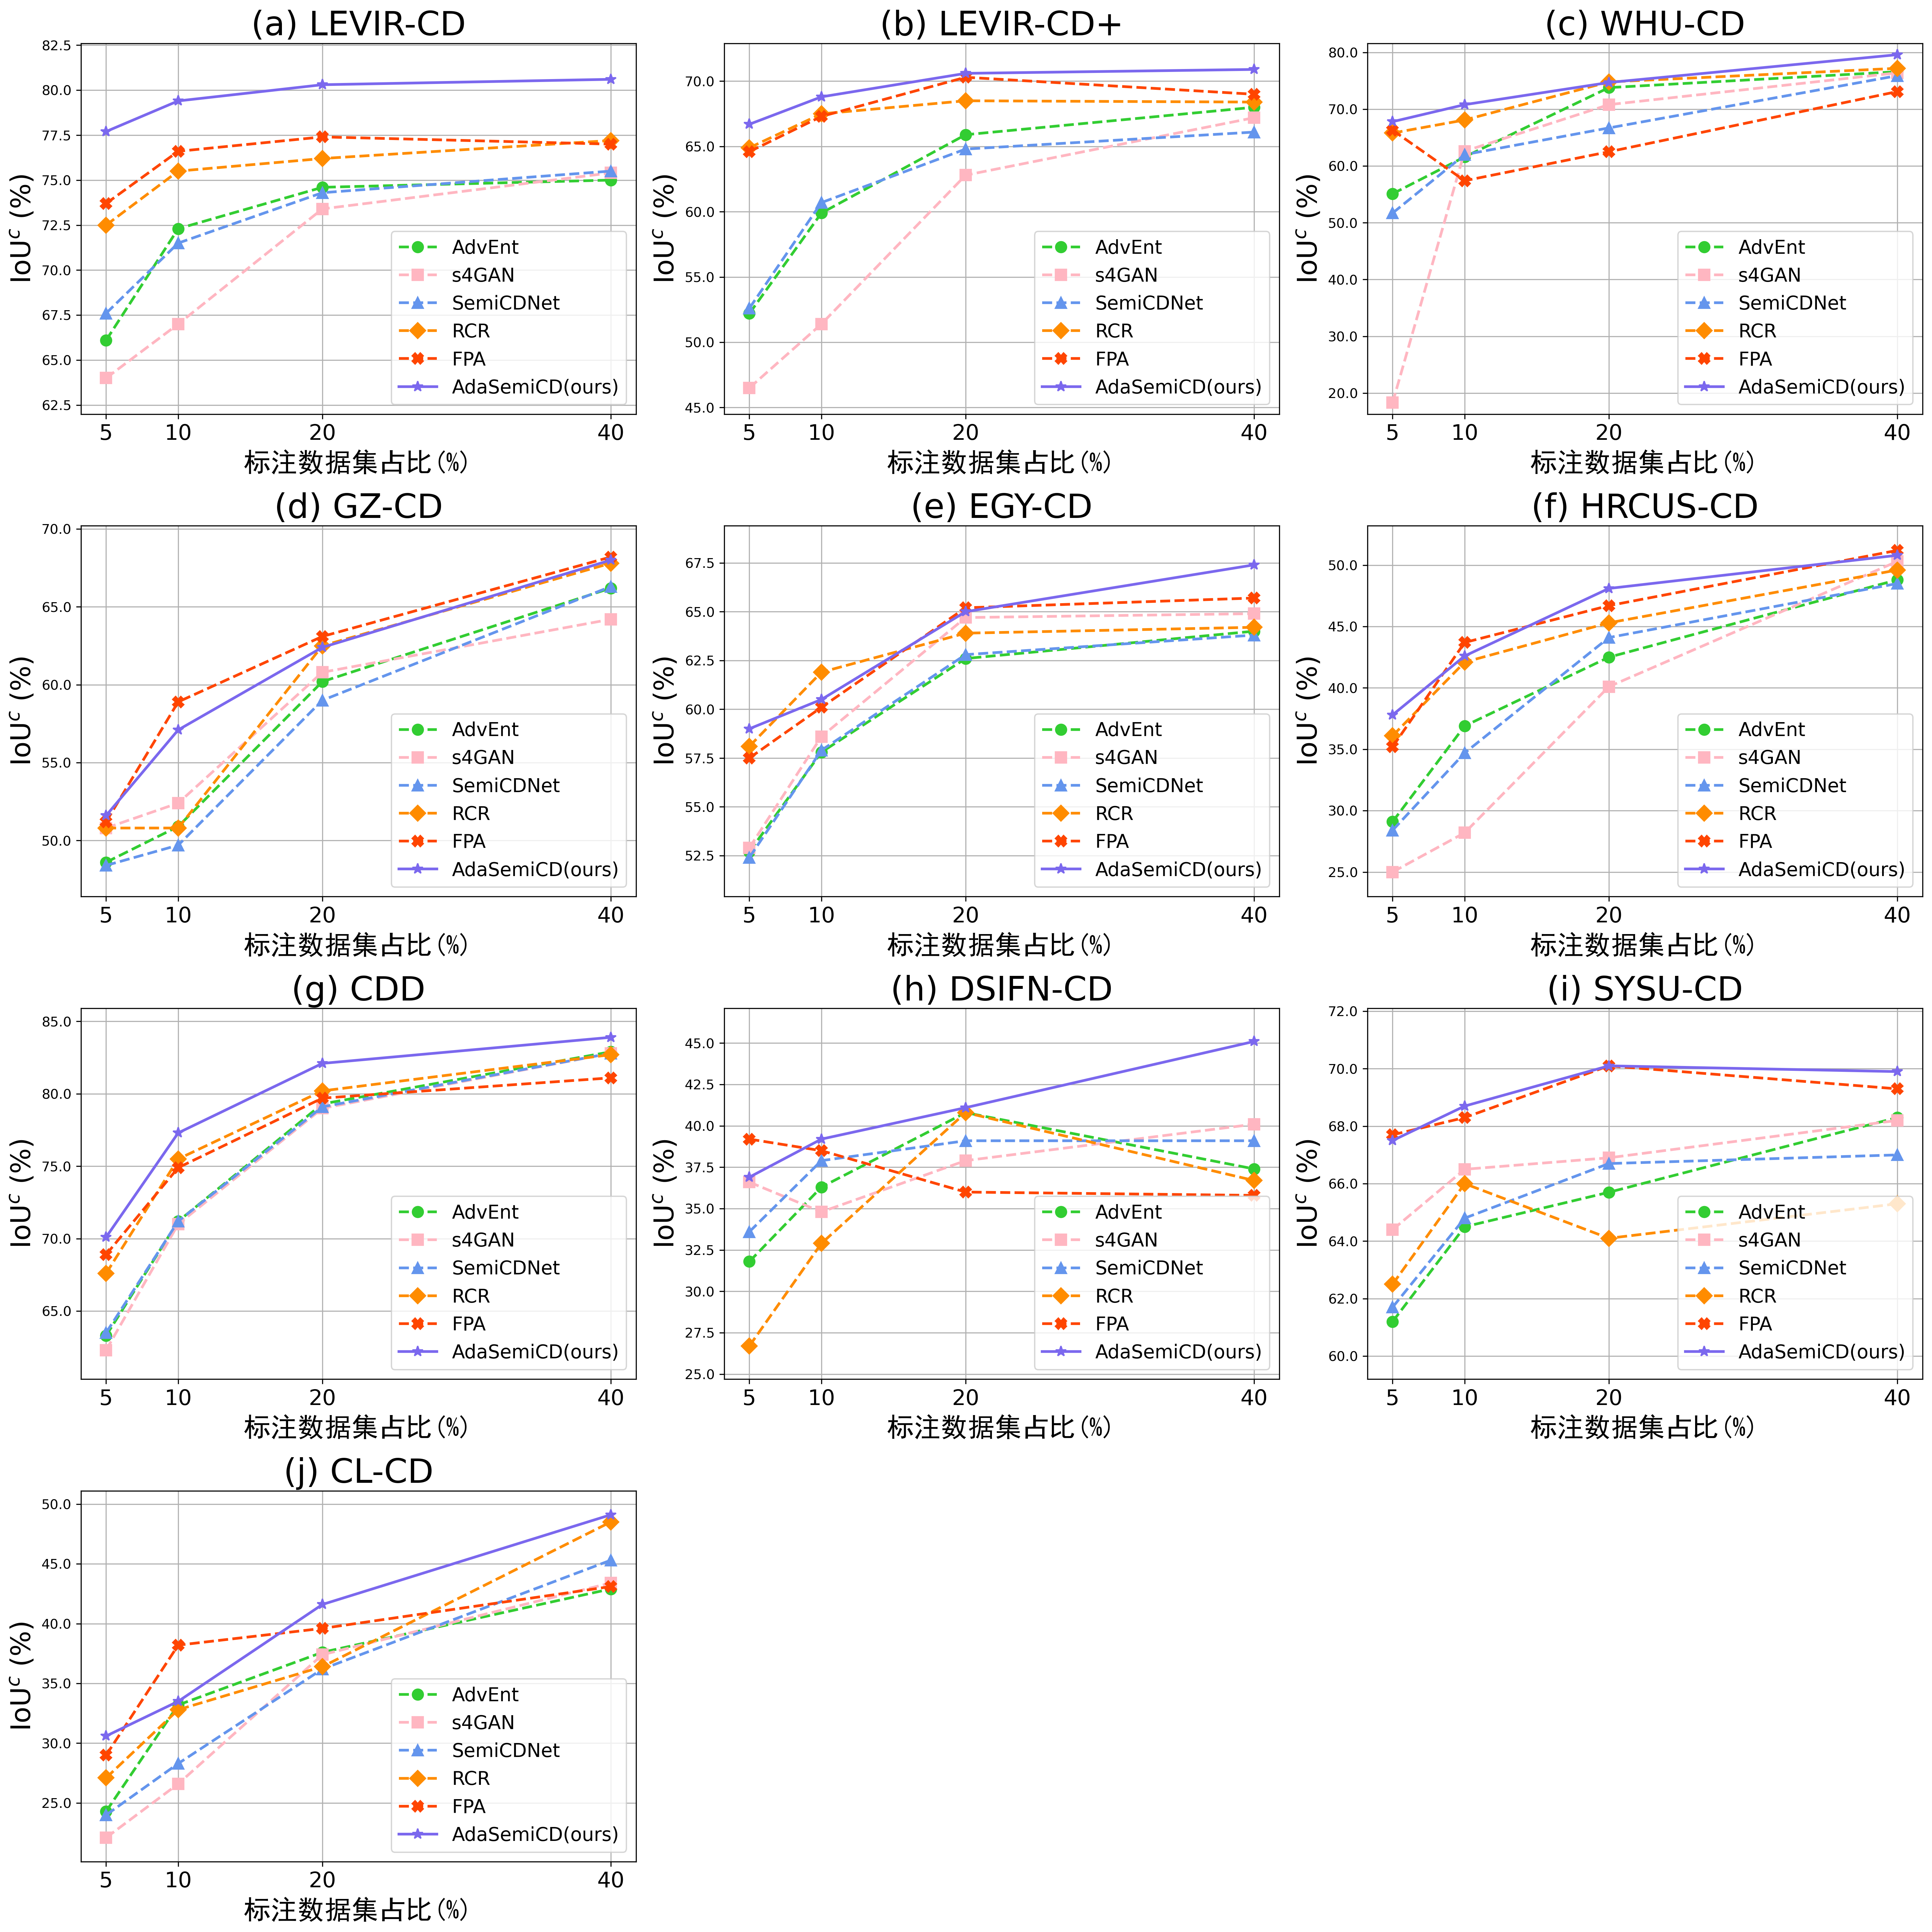
\includegraphics[scale=0.30]{images/Adavis_plot.png}
  \caption{
    AdaSemiCD与SOTA方法在10个数据集上的性能对比折线图
  }
  \label{fig:Adaiou_plot}
\end{figure}
我们在所有10个数据集上进行了实验,表\ref{tab:Ada-building}和表\ref{tab:Ada-mutil}分别报告了我们在建筑物变化检测数据集和多类变化检测数据集上的实验结果。其中,表中的Sup.Only是指仅在有限的标记数据集上进行监督训练,而Oracle是在整个全部训练数据集上进行全监督训练的结果。另外图\ref{fig:Adaiou_plot}更直观地展示了我们的所有实验定量结果。值得注意的是,我们的方法在所有数据集的几乎所有半监督划分设置中都实现了最先进的性能。可以肯定的是,在大多数情况下,所有的半监督变化检测方法在相应的划分设置下都比监督方法表现得更好,这证明了半监督方法在从大量未标记的训练样本中学习到了更多的知识,同时,我们的方法取得的领先证明了我们对于如何高效、正确地从未标记样本集中学习的自适应机制是具有实际意义的。
\begin{table}[!htbp]
  \centering
  % \tiny
  \scriptsize
  \caption{不同CD方法在二值建筑物变化检测数据集上的平均定量性能对比}
  \resizebox{0.9\textwidth}{!}{
  \begin{tabular}{p{20mm}p{25mm}p{8mm}p{8mm}cp{8mm}p{8mm}cp{8mm}p{8mm}cp{8mm}p{8mm}} %
      \toprule
      \multirow{2}{*}{Dataset} & \multirow{2}{*}{\parbox[c]{.2\linewidth}{Method}} & \multicolumn{2}{c}{5\%} & & \multicolumn{2}{c}{10\%} & & \multicolumn{2}{c}{20\%} & & \multicolumn{2}{c}{40\%}\\
      \cmidrule{3-4} \cmidrule{6-7} \cmidrule{9-10} \cmidrule{12-13}
      & & {$IoU^c$} & {OA} && {$IoU^c$} & {OA} & & {$IoU^c$} & {OA} &&{$IoU^c$} & {OA}\\
      \midrule
      \multirow{8}{*}{LEVIR-CD}
      & Sup. only   &   61.0 & 97.60 && 66.8 & 98.13 && 72.3 & 98.44 && 74.9 & 98.60 \\ %40
      & AdvEnt\cite{vu2019advent}& 66.1 & 98.08 && 72.3 & 98.45 && 74.6 & 98.58 && 75.0 & 98.60 \\ %40
      & s4GAN\cite{mittal2019semi}& 64.0 & 97.89 && 67.0 & 98.11 && 73.4 & 98.51 && 75.4 & 98.62 \\
      & SemiCDNet\cite{peng2021SemiCDNet} & 67.6 & 98.17 && 71.5 & 98.42 && 74.3 & 98.58 && 75.5 & 98.63 \\ %40
      & RCR\cite{bandara2022RCR}& 72.5 & 98.47 && 75.5 & 98.63 && 76.2 & 98.68 && 77.2 & 98.72 \\
      & FPA\cite{Zhang2023FPA}& \underline{73.7} & \underline{98.57} && \underline{76.6} & \underline{98.72} && \underline{77.4} & \underline{98.75} && \underline{77.0} & \underline{98.74} \\
      \rowcolor{mycyan}
      \multirow{-8}{*}{\cellcolor{white}}& \cellcolor{white}AdaSemiCD   &   \textbf{77.7} & \textbf{98.78} && \textbf{79.4} & \textbf{98.87} && \textbf{80.3} & \textbf{98.92} && \textbf{80.6} & \textbf{98.93} \\%40
      \cline{2-13}
      & Oracle & \multicolumn{11}{c}{$ IoU^c$=\textcolor{red}{\bf 77.9} and OA=\textcolor{red}{\bf 98.77}} \\
      \bottomrule
      %\midrule
      \multirow{8}{*}{LEVIR-CD+}
      & Sup. only   &   52.0 & 97.72 && 58.4 & 98.06 && 66.1 & 98.31 && 66.2 & 98.42 \\ %40
      & AdvEnt\cite{vu2019advent}& 52.2 & 97.68 && 59.9 & 98.11 && 65.9 & 98.37 && 68.0 & 98.51 \\ %40
      & s4GAN\cite{mittal2019semi}& 46.5 & 97.25 && 51.4 & 97.66 && 62.8 & 98.18 && 67.2 & 98.46 \\
      & SemiCDNet\cite{peng2021SemiCDNet} & 52.6 & 97.66 && 60.7 & 98.24 && 64.8 & 98.37 && 66.1 & 98.38 \\ %40
      & RCR\cite{bandara2022RCR}& \underline{64.9} & 98.25 && \underline{67.5} & \underline{98.45} && 68.5 & 98.52 && 68.4 & 98.51 \\
      & FPA\cite{Zhang2023FPA}& 64.6 & \underline{98.30} && 67.3 & 98.40 && \underline{70.3} & \cellcolor{mycyan}\textbf{98.64} && \underline{69.0} & \underline{98.59} \\
      \rowcolor{mycyan}
      \multirow{-8}{*}{\cellcolor{white}}& \cellcolor{white}AdaSemiCD   &   \textbf{66.7} & \textbf{98.49} && \textbf{68.8} & \textbf{98.51} && \textbf{70.6} & \cellcolor{white}\underline{98.63} && \textbf{70.9} & \textbf{98.64} \\%40
      \cline{2-13}
      & Oracle & \multicolumn{11}{c}{$ IoU^c$=\textcolor{red}{\bf 70.5} and OA=\textcolor{red}{\bf 98.63}} \\
      \bottomrule
      % \midrule
      \multirow{8}{*}{WHU-CD}
      & Sup. only   &   50.0 & 97.48 && 55.7 & 97.53 && 65.4 & 98.20 && 76.1 & 98.94 \\ %40
      & AdvEnt\cite{vu2019advent}& 55.1 & 97.90 && 61.6 & 98.11 && 73.8 & 98.80 && 76.6 & 98.94 \\ %40
      & s4GAN\cite{mittal2019semi}& 18.3 & 96.69 && 62.6 & 98.15 && 70.8 & 98.60 && 76.4 & 98.96 \\
      & SemiCDNet\cite{peng2021SemiCDNet} & 51.7 & 97.71 && 62.0 & 98.16 && 66.7 & 98.28 && 75.9 & 98.93 \\ %40
      & RCR\cite{bandara2022RCR}& 65.8 & 98.37 && \underline{68.1} & \underline{98.47} && \cellcolor{mycyan}\textbf{74.8} & \underline{98.84} && \underline{77.2} & \underline{98.96} \\
      & FPA\cite{Zhang2023FPA}& \underline{66.3} & \underline{98.45} && 57.4 & 97.69 && 62.5 & 98.48 && 73.1 & 98.69 \\
      \rowcolor{mycyan}
      \multirow{-8}{*}{\cellcolor{white}}& \cellcolor{white}AdaSemiCD   &   \textbf{67.8} & \textbf{98.62} && \textbf{70.8} & \textbf{98.70} && \cellcolor{white}\underline{74.7} & \textbf{98.86} && \textbf{79.6} & \textbf{99.13} \\%40
      \cline{2-13}
      & Oracle & \multicolumn{11}{c}{$ IoU^c$=\textcolor{red}{\bf 85.5} and OA=\textcolor{red}{\bf 99.38}} \\
      \bottomrule
      % \midrule
      \multirow{8}{*}{GZ-CD}
      & Sup. only   &   47.5 & 93.56 && 51.4 & 94.26 && 58.0 & 95.65 && 66.3 & 96.62 \\ %40
      & AdvEnt\cite{vu2019advent}& 48.6 & 94.39 && 50.9 & 94.89 && 60.2 & 95.79 && 66.2 & 96.58 \\ %40
      & s4GAN\cite{mittal2019semi}& 50.8 & 94.38 && 52.4 & 94.98 && 60.8 & 95.94 && 64.2 & 96.39 \\
      & SemiCDNet\cite{peng2021SemiCDNet} & 48.4 & 93.58 && 49.7 & 94.79 && 59.0 & 95.66 && 66.3 & 96.57 \\ %40
      & RCR\cite{bandara2022RCR}& 50.8 & 93.82 && 50.8 & 94.69 && 62.5 & 96.07 && 67.8 & 96.61 \\
      \rowcolor{mycyan}
      \multirow{-7}{*}{\cellcolor{white}}& \cellcolor{white}
      FPA\cite{Zhang2023FPA}& \cellcolor{white}51.2 & \cellcolor{white}93.92 && \textbf{58.9} & \textbf{95.78} && \textbf{63.1} & \textbf{96.26} && \textbf{68.2} & \textbf{96.82} \\
      \multirow{-8}{*}{\cellcolor{white}}& \cellcolor{white}AdaSemiCD   &   \cellcolor{mycyan}\textbf{51.6} & \cellcolor{mycyan}\textbf{94.56} && \underline{57.1} & \underline{95.57} && \underline{62.4} & \underline{96.21} && \underline{68.0} & \underline{96.75} \\%40
      \cline{2-13}
      & Oracle & \multicolumn{11}{c}{$ IoU^c$=\textcolor{red}{\bf 69.0} and OA=\textcolor{red}{\bf 96.93}} \\
      \bottomrule
      \multirow{8}{*}{EGY-CD}
      & Sup. only   &   49.8 & 95.73 && 54.6 & 96.38 && 61.4 & 96.83 && 65.1 & 97.25 \\ %40
      & AdvEnt\cite{vu2019advent}& 52.7 & 96.01 && 57.8 & 96.58 && 62.6 & 96.86 && 64.0 & 97.19 \\ %40
      & s4GAN\cite{mittal2019semi}& 52.9 & 95.94 && 58.6 & 96.50 && 64.7 & 97.09 && 64.9 & 97.27 \\
      & SemiCDNet\cite{peng2021SemiCDNet} & 52.4 & 96.00 && 57.9 & 96.31 && 62.8 & 96.95 && 63.8 & 97.19 \\ %40
      & RCR\cite{bandara2022RCR}& \underline{58.1} & 96.50 && \underline{61.9} & 96.77 && 63.9 & 97.08 && 64.2 & 97.18 \\

      \multirow{-7}{*}{\cellcolor{white}}& \cellcolor{white}
      FPA\cite{Zhang2023FPA}& 57.5 & \underline{96.52} && 60.1 & \cellcolor{mycyan}\textbf{96.86} &\cellcolor{mycyan}& \cellcolor{mycyan}\textbf{65.2} & \cellcolor{mycyan}\textbf{97.25} && \underline{65.7} & \underline{97.34} \\

      \rowcolor{mycyan}
      \multirow{-8}{*}{\cellcolor{white}}& \cellcolor{white}AdaSemiCD   &   \textbf{59.0} & \textbf{96.55} && \textbf{60.5} & \cellcolor{white}\underline{96.80} & \cellcolor{white} & \cellcolor{white}\underline{65.0} & \cellcolor{white}\underline{97.20} & \cellcolor{white}& \textbf{67.4} & \textbf{97.39} \\%40
      \cline{2-13}
      & Oracle & \multicolumn{11}{c}{$ IoU^c$=\textcolor{red}{\bf 67.6} and OA=\textcolor{red}{\bf 97.54}} \\
      \bottomrule
      \multirow{8}{*}{HRCUS-CD}
      & Sup. only   &   29.5 & 98.11 && 36.0 & 98.45 && 43.4 & 98.68 && 48.9 & 98.84 \\ %40
      & AdvEnt\cite{vu2019advent}& 29.1 & 98.11 && 36.9 & 98.40 && 42.5 & 98.61 && 48.8 & 98.71 \\ %40
      & s4GAN\cite{mittal2019semi}& 25.0 & 97.86 && 28.2 & 98.24 && 40.1 & 98.62 && 50.3 & 98.85 \\
      & SemiCDNet\cite{peng2021SemiCDNet} & 28.4 & 98.00 && 34.7 & 98.44 && 44.1 & 98.68 && 48.5 & 98.74 \\ %40
      & RCR\cite{bandara2022RCR}& \underline{36.1} & 98.36 && 42.1 & \underline{98.69} && 45.3 & 98.76 && 49.6 & 98.66 \\

      & FPA\cite{Zhang2023FPA}& 35.2 & \underline{98.37} && \cellcolor{mycyan}\textbf{43.7} & 98.65 && \underline{46.7} & \underline{98.82} && \cellcolor{mycyan}\textbf{51.2} & \textbf{98.81} \\

      \rowcolor{mycyan}
      \multirow{-8}{*}{\cellcolor{white}}& \cellcolor{white}AdaSemiCD   &  \textbf{37.8} & \cellcolor{mycyan}\textbf{98.59} && \cellcolor{white}\underline{42.6} & \textbf{98.70} && \textbf{48.1} & \textbf{98.84} && \cellcolor{white}\underline{50.8} & \underline{98.87} \\%40
      \cline{2-13}
      & Oracle & \multicolumn{11}{c}{$ IoU^c$=\textcolor{red}{\bf 59.0} and OA=\textcolor{red}{\bf 99.06}} \\
      \bottomrule
  \end{tabular}
  }
  \label{tab:Ada-building}
\end{table}

\textbf{建筑物变化检测}:
如表\ref{tab:Ada-building}所示,其中蓝色高亮部分代表着最优结果,下划线标注的是次优结果。我们所提出的AdaSemiCD框架在几乎所有建筑物变化检测数据集上都表现出了出色的性能。值得注意的是,在LEVIR-CD、LEVIR-CD+和WHU-CD数据集上,AdaSemiCD在$IoU^c$上实现了全面的、显著的改进,分别提高了3.1、1.3和1.7个百分点。在EGY-CD和HRCUS-CD数据集上,AdaSemiCD总体上相较于之前的最佳方法有所提升,分别平均提高了0.75和0.4个百分点。然而,在某些实验设置下,其性能略低于之前表现最好的方法。这可以归因于这些数据集带来的独特挑战:EGY-CD数据集存在大量的过度曝光问题,这经常导致建筑物与背景混合在一起,增加了准确区分的难度。同样,HRCUS-CD数据集也受到了某些建筑物变化区域存在的植被遮挡的影响。这些挑战阻碍了模型在用有限的真实标签进行训练时生成可靠的伪标签的能力。

显然,AdaSemiCD在GZ-CD数据集上遇到了严峻的挑战,除了在5$\%$标记率的半监督设置下保持领先之外,其余大多数实验设置下的性能表现都逊于FPA。我们将其归因于该数据集的固有特性和我们方法的固有局限性。首先,在所有进行实验的数据集中,GZ-CD数据集的空间分辨率最低。这种限制,再加上小建筑物的普遍存在,导致在这种分辨率下很难准确辨别出变化目标,即使是对人类观察者用肉眼来检测也是如此。其次,该数据集的人工注释非常粗糙,当然这也与我们前边的推测相同。如图\ref{fig:building_sample}所示,对于具有多个目标的区域,Ground Truth中通常是直接将一整块直接标注为变化区域,而这其中包含大部分背景区域。这会在标记的数据中引入大量噪声,特别是对于建筑物变化检测任务。最后,数据集采集的背景也带来了额外的挑战,该数据集采集于城市郊区,而在超过五年的时间跨度内,城市的快速发展和扩张导致了前后两幅时相的图像之间存在巨大差异,除了带注释的建筑变化区域之外。背景的变化也非常显著,例如整片区域的植被变为裸土,以至于很难确定两幅图像之间的关系,这引入了大量非目标类别变化,严重干扰了模型关注建筑物变化区域的能力。然而,与AdaSemiCD不同,FPA和RCR并不完全依赖单一硬标签。相反,它们利用特征一致性约束指导模型训练,这很大程度上有效地缓解了这个问题。

此外,从实验结果来看,由于背景类占多数,所有方法在这些二值建筑物变化检测数据集上的总体准确率(OA)都很高。OA往往直接映射着平均交并比$IoU^c$, 即便是小幅度的OA提升,$IoU^c$就会有比较明显的改善。我们的AdaSemiCD在几乎所有的数据集上都取得了提高,因为它有效地降低了噪声,最大限度地减少了错误信号的影响,从而在像素级实现了更准确的预测。

\textbf{多类变化检测}:
值得注意的是,在CDD数据集的所有实验设置上都取得了最优的结果,IoUc和OA分别平均增加了1.8个百分点和0.25个百分点,这可以归因于其异常准确的标注,如图3所示。这种高质量的标注对于基于伪标签的半监督方法特别有利。此外,AdaSemiCD在SYSU-CD和CL-CD数据集上的整体性能有所提高。然而,在某些实验配置中,它的性能略低于SOTA结果。这可以归因于在识别这些数据集中存在的一些山脉和土地变化方面的固有挑战。这些变化通常是大规模的,这些地区的错误分类可能会导致性能指标的波动。
\begin{table}[H]
  \centering
  % \tiny
  \scriptsize
  \caption{不同CD方法在多类变化检测数据集上的平均定量性能对比}
  \resizebox{0.9\textwidth}{!}{
  \begin{tabular}{p{20mm}p{25mm}p{8mm}p{8mm}cp{8mm}p{8mm}cp{8mm}p{8mm}cp{8mm}p{8mm}} %
      \toprule
      \multirow{2}{*}{Dataset} & \multirow{2}{*}{\parbox[c]{.2\linewidth}{Method}} & \multicolumn{2}{c}{5\%} & & \multicolumn{2}{c}{10\%} & & \multicolumn{2}{c}{20\%} & & \multicolumn{2}{c}{40\%}\\
      \cmidrule{3-4} \cmidrule{6-7} \cmidrule{9-10} \cmidrule{12-13}
      & & {$IoU^c$} & {OA} && {$IoU^c$} & {OA} & & {$IoU^c$} & {OA} &&{$IoU^c$} & {OA}\\
      \midrule
      \multirow{8}{*}{CDD-CD}
      & Sup. only   &   60.4 & 94.25 && 67.9 & 95.46 && 75.6 & 96.59 && 82.3 & 97.56 \\ %40
      & AdvEnt\cite{vu2019advent}& 63.3 & 94.65 && 71.2 & 96.01 && 79.3 & 97.14 && \underline{82.9} & \underline{97.66} \\ %40
      & s4GAN\cite{mittal2019semi}& 62.3 & 94.69 && 71.0 & 95.94 && 79.0 & 97.10 && 82.8 & 97.63 \\
      & SemiCDNet\cite{peng2021SemiCDNet} & 63.5 & 94.68 && 71.2 & 95.99 && 79.1 & 97.13 && 82.8 & 97.63 \\ %40
      & RCR\cite{bandara2022RCR}& 67.6 & 95.40 && \underline{75.5} & \underline{96.57} && \underline{80.2} & \underline{97.26} && 82.7 & 97.61 \\
      & FPA\cite{Zhang2023FPA}& \underline{68.9} & \underline{95.66} && 74.9 & 96.55 && 79.7 & 97.20 && 81.1 & 97.37 \\
      \rowcolor{mycyan}
      \multirow{-8}{*}{\cellcolor{white}}& \cellcolor{white}AdaSemiCD   &   \textbf{70.1} & \textbf{95.89} && \textbf{77.3} & \textbf{96.89} && \textbf{82.1} & \textbf{97.56} && \textbf{83.9} & \textbf{97.80} \\%40
      \cline{2-13}
      & Oracle & \multicolumn{11}{c}{$ IoU^c$=\textcolor{red}{\bf 87.8} and OA=\textcolor{red}{\bf 98.10}} \\
      \bottomrule
      %\midrule
      \multirow{8}{*}{DSIFN-CD}
      & Sup. only   &   34.8 & 78.34 && \underline{38.9} & 83.41 && 40.2 & 87.00 && 39.6 & 87.00 \\ %40
      & AdvEnt\cite{vu2019advent}& 31.8 & 77.83 && 36.3 & 83.86 && 40.8 & 85.92 && 37.4 & 86.31 \\ %40
      & s4GAN\cite{mittal2019semi}& 36.6 & \underline{84.10} && 34.8 & \underline{86.87} && 37.9 & \cellcolor{mycyan}\textbf{87.69} && \underline{40.1} & 86.52 \\
      & SemiCDNet\cite{peng2021SemiCDNet} & 33.6 & 78.60 && 37.9 & 84.18 && 39.1 & 86.77 && 39.1 & \underline{87.05} \\ %40
      & RCR\cite{bandara2022RCR}& 26.7 & 83.78 && 32.9 & 86.05 && 40.8 & 86.70 && 36.7 & 86.08 \\
      & FPA\cite{Zhang2023FPA}& \cellcolor{mycyan}\textbf{39.2} & \cellcolor{mycyan}\textbf{84.27} && 38.5 & \cellcolor{mycyan}\textbf{87.12} && 36.0 & \underline{87.41} && 35.8 & 86.50 \\
      % \rowcolor{mycyan}
      \multirow{-8}{*}{\cellcolor{white}}& \cellcolor{white}AdaSemiCD   &   \cellcolor{white}\underline{36.9} & \cellcolor{white}80.46 && \cellcolor{mycyan}\textbf{39.2} & 82.94 && \cellcolor{mycyan}\textbf{41.1} & 85.45 && \cellcolor{mycyan}\textbf{45.1} & \cellcolor{mycyan}\textbf{87.12} \\%40
      \cline{2-13}
      & Oracle & \multicolumn{11}{c}{$ IoU^c$=\textcolor{red}{\bf 58.1} and OA=\textcolor{red}{\bf 90.82}} \\
      \bottomrule
      % \midrule
      \multirow{8}{*}{SYSU-CD}
      & Sup. only   &   62.9 & 89.57 && 64.4 & 90.18 && 66.0 & 90.82 && 66.4 & 90.93 \\ %40
      & AdvEnt\cite{vu2019advent}& 61.2 & 89.36 && 64.5 & 90.18 && 65.7 & 90.35 && 68.3 & 91.24 \\ %40
      & s4GAN\cite{mittal2019semi}& 64.4 & 90.02 && 66.5 & 90.48 && 66.9 & 90.26 && 68.2 & 91.51 \\
      & SemiCDNet\cite{peng2021SemiCDNet} & 61.7 & 89.32 && 64.8 & 90.25 && 66.7 & 90.97 && 67.0 & 91.08 \\ %40
      & RCR\cite{bandara2022RCR}& 62.5 & 89.76 && 66.0 & 90.75 && 64.1 & 90.22 && 65.3 & 90.56 \\
      & FPA\cite{Zhang2023FPA}& \cellcolor{mycyan}\textbf{67.7} & 90.95 && \underline{68.3} & \underline{91.09} && \underline{70.1} & \underline{92.01} && \underline{69.3} & \cellcolor{mycyan}\textbf{91.97} \\
      \rowcolor{mycyan}
      \multirow{-8}{*}{\cellcolor{white}}& \cellcolor{white}AdaSemiCD   &   \cellcolor{white}\underline{67.5} & \textbf{91.16} && \textbf{68.7} & \textbf{91.59} && \textbf{70.1} & \textbf{92.03} && \textbf{69.9} & \cellcolor{white}\underline{91.90} \\%40
      \cline{2-13}
      & Oracle & \multicolumn{11}{c}{$ IoU^c$=\textcolor{red}{\bf 68.2} and OA=\textcolor{red}{\bf 91.64}} \\
      \bottomrule
      % \midrule
      \multirow{8}{*}{CL-CD}
      & Sup. only   &   18.1 & 91.90 && 31.4 & 92.42 && 37.2 & 93.32 && 45.9 & \underline{94.98} \\ %40
      & AdvEnt\cite{vu2019advent}& 24.3 & 92.13 && 33.2 & 93.01 && 37.6 & 93.59 && 42.9 & 94.06 \\ %40
      & s4GAN\cite{mittal2019semi}& 22.1 & 92.00 && 26.6 & 93.09 && 37.4 & 93.59 && 43.4 & 93.87 \\
      & SemiCDNet\cite{peng2021SemiCDNet} & 24.0 & \underline{92.20} && 28.3 & \underline{93.42} && 36.2 & 92.41 && 45.3 & 94.22 \\ %40
      & RCR\cite{bandara2022RCR}& 27.1 & 91.63 && 32.8 & 92.99 && 36.4 & 93.07 && \underline{48.5} & 94.94 \\
      & FPA\cite{Zhang2023FPA}& \underline{29.0} & 91.00 && \cellcolor{mycyan}\textbf{38.2} & \cellcolor{mycyan}\textbf{93.37} && \underline{39.6} & \underline{93.88} && 43.1 & 94.15 \\
      \rowcolor{mycyan}
      \multirow{-8}{*}{\cellcolor{white}}& \cellcolor{white}AdaSemiCD   &   \textbf{30.6} & \textbf{92.52} && \cellcolor{white}\underline{33.5} & \cellcolor{white}{92.40} && \textbf{41.6} & \textbf{94.21} && \textbf{49.1} & \textbf{95.85} \\%40
      \cline{2-13}
      & Oracle & \multicolumn{11}{c}{$ IoU^c$=\textcolor{red}{\bf 50.1} and OA=\textcolor{red}{\bf 95.55}} \\
      \bottomrule
  \end{tabular}
  }
  \label{tab:Ada-mutil}
\end{table}

如表\ref{tab:Ada-mutil}所示,我们的AdaSemiCD同样在几乎所有多类数据集和所有划分设置上都实现了最佳性能,只是提升程度低于在简单的建筑物变化检测数据集上所取得的,这是由于多类别变化检测任务本身的复杂性,最明显的一点是,在某些情况下,之前的一些半监督的变化检测方法完全失效了,比监督基线的检测性能更差。然而,我们的半监督变化检测方法仍然可以利用额外的未标记样本来提高性能。值得注意的是,在CDD数据集的所有实验设置下AdaSemiCD都取得了最优的结果,$IoU^c$和$OA$分别平均提高了1.8和0.25个百分点,这可以归因于其准确的手工标注,如图\ref{fig:mutil_sample}所示。这种高质量的标注对基于伪标签自训练的半监督方法极为有利。此外,AdaSemiCD在SYSU-CD和CL-CD数据集上的整体性能有所提高。然而,在某些实验配置中,它的性能略低于最优结果。这可以归因于在识别这些数据集中存在的一些山脉或土地变化方面的固有挑战。这些变化通常是大规模的,这些地区的错误分类可能会导致性能指标的波动。

另一点值得注意的是,在这些多类变化检测数据集中,所有方法的整体精度都降低了,$OA$和$IoU^c$不再直接对应。其中一个现象是$IoU^c$达到了最高,而OA没有,这是由于其侧重点不同。OA更注重全局精度,在背景类占主导的数据集下就是优先背景类的检测,而$IoU^c$更关注目标类别的检测,在变化检测中我们更加关注于目标对象的检测,因此$IoU^c$更加重要。从DSIFN-CD数据集的实验结果中可以看到,我们的方法在一些设置下尽管在$OA$上表现不佳,但是在$IoU^c$上取得了最好的结果。

在所有此类数据集中,我们的方法在DSIFN-CD上表现出最差的性能。虽然它在关键指标$IoU^c$上表现良好,但在$OA$上的表现并不是最优的。这可以归因于DSIFN-CD和GZ-CD的相似之处,因为这两个数据集都具有人工标注粗糙和低空间分辨率这两个特点,如图\ref{fig:mutil_sample}所示。此外,DSIFN-CD类别不平衡现象基本消失,如图\ref{fig:Adasemicd_imbalance}所示,其变化类别的比例高达34.81$\%$。因此,我们设计的类别重平衡策略的增益有限,并且可能导致预测向前景倾斜,从而对背景像素预测错误,这或许就是$OA$表现不佳的直接原因。
\subsection{定性对比}
\begin{figure}[!htbp]
  \centering
  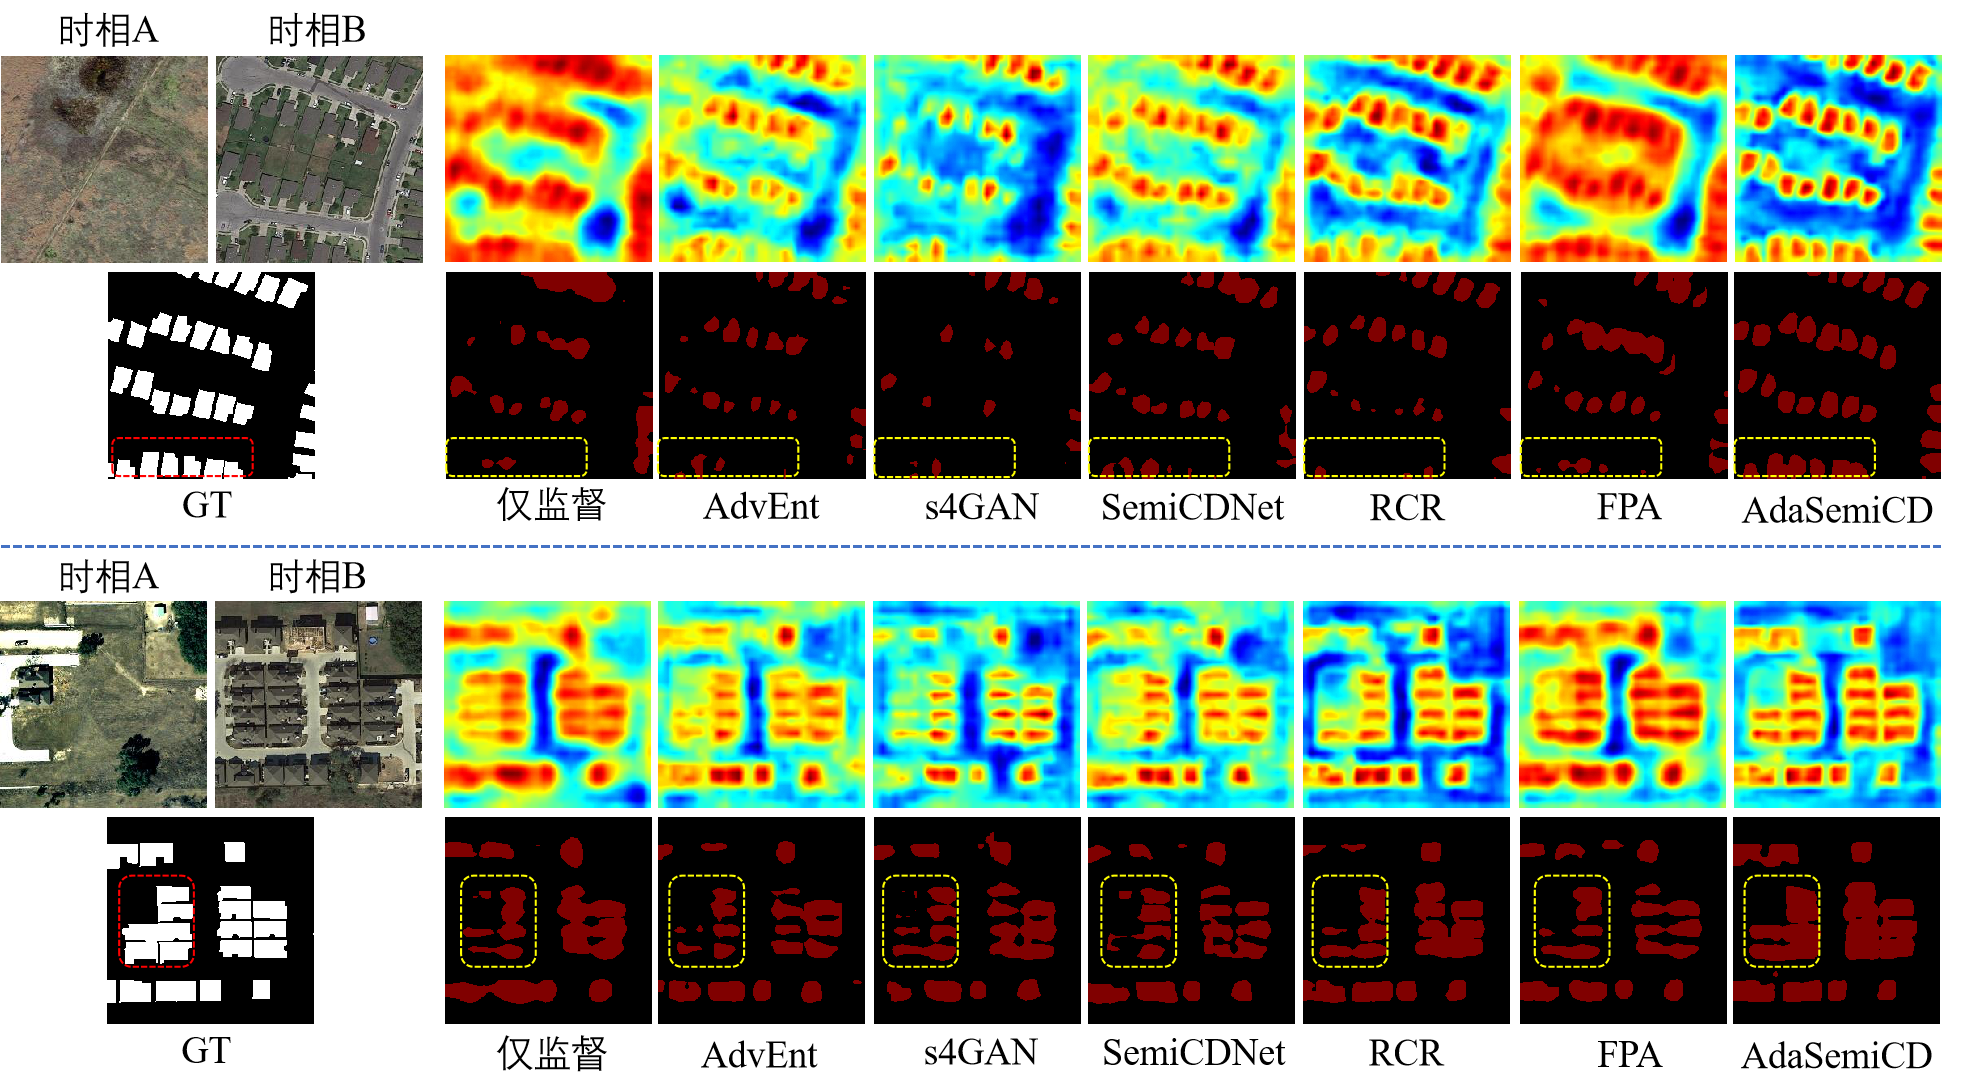
\includegraphics[scale=0.45]{images/Adalevir-vis.png}
  \caption{
    AdaSemiCD与SOTA方法在LEVIR-CD测试集上的变化检测结果可视化对比
  }
  \label{fig:AdaLevir-vis}
\end{figure}
\begin{figure}[!htbp]
  \centering
  \includegraphics[scale=0.45]{images/Adawhu-vis.png}
  \caption{
    AdaSemiCD与SOTA方法在WHU-CD测试集上的变化检测结果可视化对比
  }
  \label{fig:AdaWhu-vis}
\end{figure}
为了更清楚地说明我们提出的方法的变化检测性能提升,我们在所有十个不同的数据集的测试集上都进行了可视化,我们展示了部分可视化样例,其中图\ref{fig:AdaLevir-vis}、图\ref{fig:AdaWhu-vis}、图\ref{fig:AdaCdd-vis}以及图\ref{fig:AdaCl-vis}分别展示了在LEVIR-CD、WHU-CD、CDD、CL-CD数据集的测试集上的预测结果可视化示例。图中用方框标注的区域是容易出错的区域。显然,在这些数据集上,我们的方法显著减少了遗漏和错误检测的常见问题。在具有挑战性的场景中,我们的方法仍然可以有效地识别出感兴趣的变化目标。
\begin{figure}[!htbp]
  \centering
  \includegraphics[scale=0.45]{images/Adacdd-vis.png}
  \caption{
    AdaSemiCD与SOTA方法在CDD测试集上的变化检测结果可视化对比
  }
  \label{fig:AdaCdd-vis}
  \end{figure}

在具有挑战性的场景下,半监督变化检测方法可能会遇到错误引导的问题,从而导致这种偏差在训练过程中被进一步放大。因此,在这种情况下,从可视化图中可以看出,一些半监督方法可能比仅监督训练的基线方法表现得更差。然而,我们的模型在训练阶段通过自适应融合,一定程度上排除了部分噪声,并在整个训练过程中自适应地集成完成进化的模型参数,在这些复杂的情况下,伪标签的质量会逐渐提高,直到它们达到可靠的标准,从而为模型训练提供准确的信号。因此,我们的方法在这些具有挑战性的领域表现出了优越的性能,如图\ref{fig:AdaWhu-vis}和图\ref{fig:AdaCdd-vis}中强调的区域。
\begin{figure}[!htbp]
  \centering
  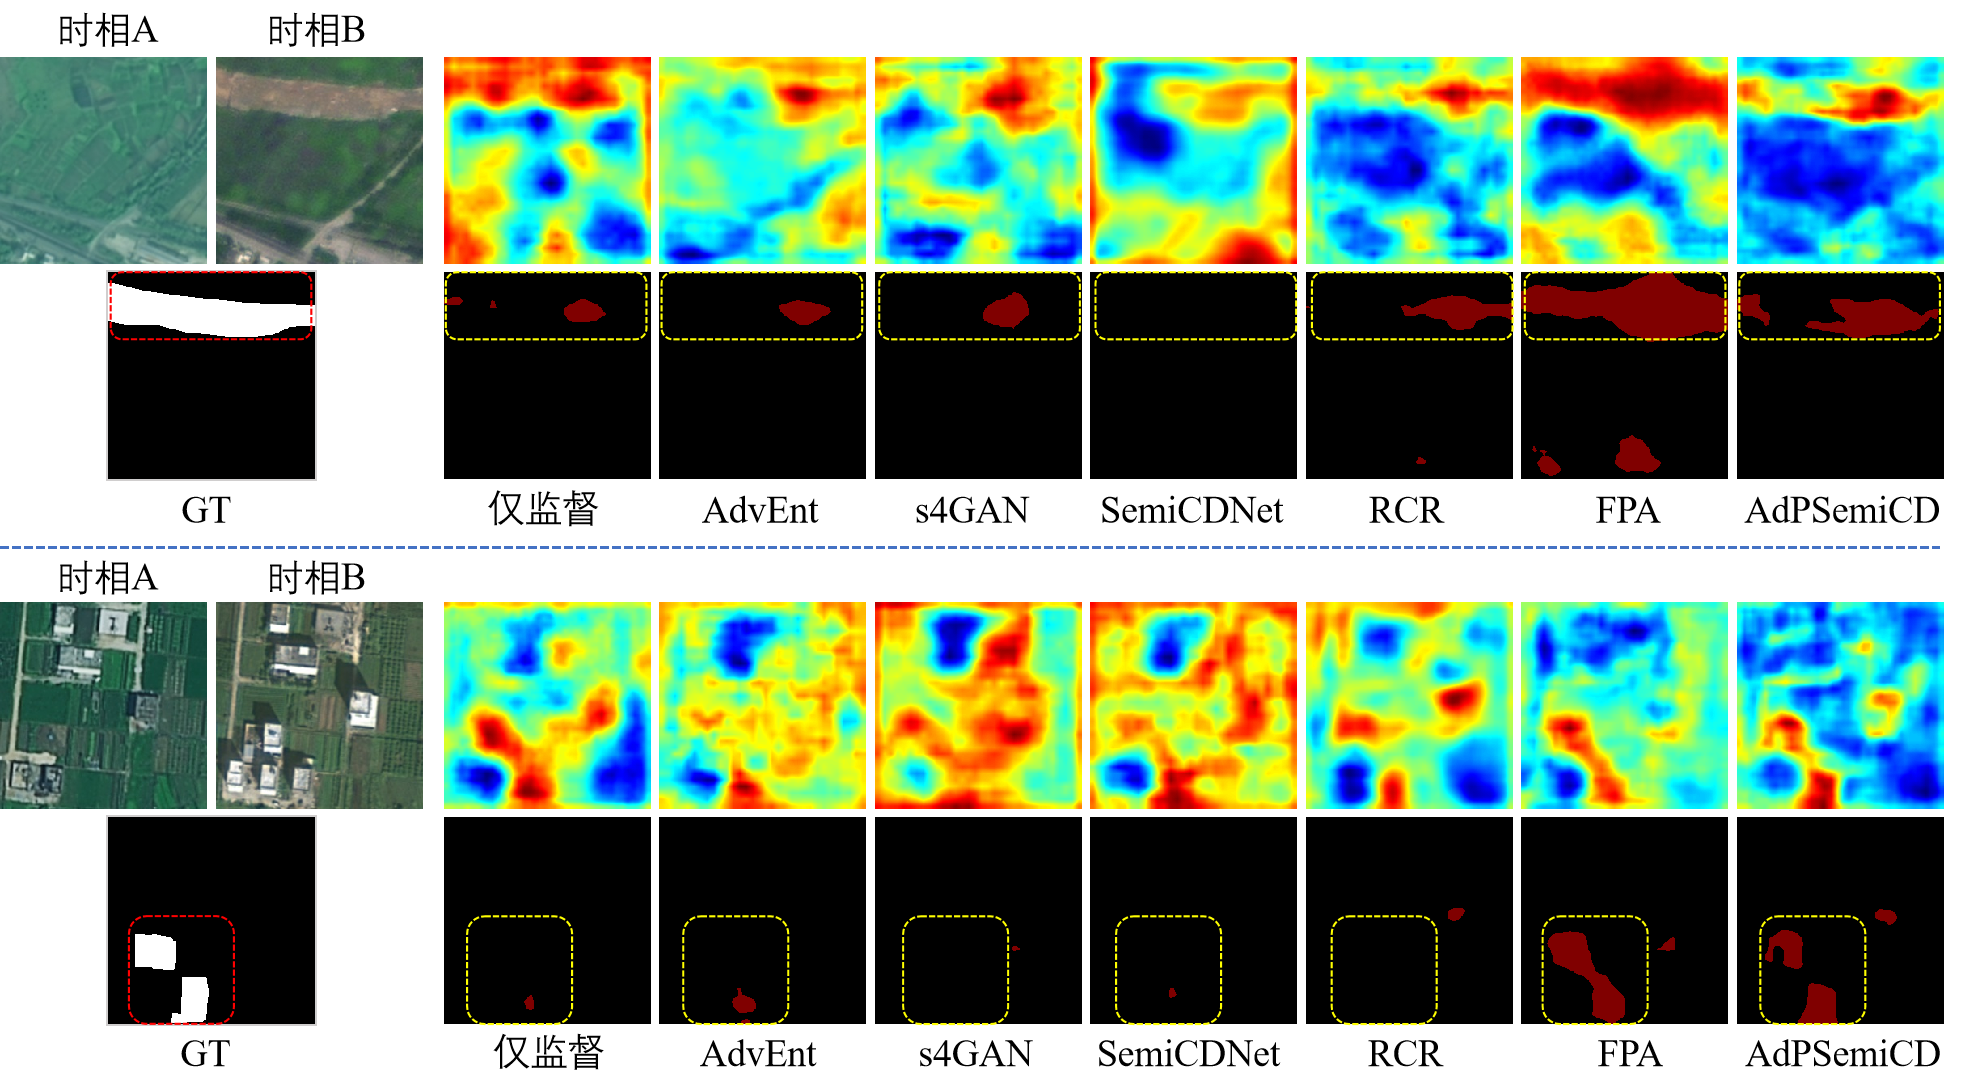
\includegraphics[scale=0.45]{images/AdaCl-vis.png}
  \caption{
    AdaSemiCD与SOTA方法在CL-CD测试集上的变化检测结果可视化对比
  }
  \label{fig:AdaCl-vis}
  \end{figure}
\subsection{消融实验}
在本小节中,我们进行了消融研究,主要是为了验证每个模块在我们提出的方法中的作用,并探索我们在实验中的一些超参数选择。

\subsubsection{自适应机制有效性}
由于对比的半监督方法与本文模型结构的差异,我们一开始并没有急于验证我们所提出的自适应机制的优越性。相反,我们首先使用经典的平均教师框架作为基线进行了实验,除了为其设置的固定超参数来控制无监督损失的权重外,其余的数据增强和变化检测网络与所有方法保持相同。与单模型和共享权值的双分支网络相比,平均教师框架的优势非常明显。这也证明了扰动一致性和移动指数平均的有效性,在此基础上我们探讨了所提出的自适应机制的效力,此实验在LEVIR-CD数据集上进行。
\begin{table*}[ht]
  % \renewcommand\arraystretch{1.2}
\centering
% \tiny
\caption{AdaSemiCD在LEVIR-CD数据集上的消融研究}
   \resizebox{0.9\textwidth}{!}{
   % \setlength{\tabcolsep}{9pt}
\begin{tabular}{p{30mm}p{20mm}p{20mm}cp{20mm}p{20mm}cp{20mm}p{20mm}cp{20mm}p{20mm}} %
  \toprule
  \multirow{2}{*}{\parbox[c]{.2\linewidth}{Method}} & \multicolumn{2}{c}{5\%} & & \multicolumn{2}{c}{10\%} & & \multicolumn{2}{c}{20\%} & & \multicolumn{2}{c}{40\%}\\
  \cmidrule{2-3} \cmidrule{5-6} \cmidrule{8-9} \cmidrule{11-12}
  & {$IoU^c$} & {OA} && {$IoU^c$} & {OA} & & {$IoU^c$} & {OA} &&{$IoU^c$} & {OA}\\
  \midrule
  仅监督   &   61.0 & 97.60 && %5
                  66.8 & 98.13 && %10
                  72.3 & 98.44 && %20
                  74.9 & 98.60 \\ %40
    MT-EMA      &   67.1 {\color{red} (+6.1)} & 98.14 {\color{red}(+0.54)} &&
                  75.0 {\color{red} (+8.2)} & 98.63 {\color{red} (+0.50)} &&
                  76.6 {\color{red} (+4.3)} & 98.71 {\color{red} (+0.27)}&&
                  77.0 {\color{red} (+2.1)} & 98.73 {\color{red} (+0.13)} \\
      MT-AEMA     &   68.9 {\color{red} (+7.9)}& 98.23 {\color{red} (+0.63)} &&
                  76.1 {\color{red} (+9.3)} & 98.66 {\color{red} (+0.53)} &&
                      77.7 {\color{red} (+5.4)} & 98.78 {\color{red} (+0.34)} &&
                  77.8 {\color{red} (+2.9)} & 98.78 {\color{red} (+0.18)} \\
      (MT-EMA)+AF* &  72.0 {\color{red} (+11.0)} & 98.43 {\color{red} (+0.83)} && %5
                  76.8 {\color{red} (+10.0)} & 98.72 {\color{red} (+0.59)} && %10
                77.5 {\color{red} (+5.2)} & 98.74 {\color{red} (+0.30)} && %20
                  78.5 {\color{red} (+3.6)} & 98.80 {\color{red} (+0.20)} \\ %40
  (MT-EMA)+AF &   77.0 {\color{red} (+16.0)} & 98.72 {\color{red} (+1.12)} && %5
                  78.8 {\color{red} (+12.0)} & 98.83 {\color{red} (+0.70)} && %10
                80.4 {\color{red} (+8.1)} & 98.91 {\color{red} (+0.47)} && %20
                  80.0 {\color{red} (+5.1)} & 98.90 {\color{red} (+0.30)} \\ %40
      AdaSemiCD   &   77.7 {\color{red} (+16.7)} & 98.78 {\color{red} (+1.18)} &&
                  79.4 {\color{red} (+12.6)} & 98.87 {\color{red} (+0.74)} &&
                  80.3 {\color{red} (+8.0)} & 98.92 {\color{red} (+0.48)} &&
                  80.6 {\color{red} (+5.7)} & 98.93 {\color{red} (+0.33)} \\
  \bottomrule
\end{tabular}
  }
% \normalsize
\label{tab:AdaModule_ablation}
\end{table*}

我们将所提出的AdaEMA模块和AdaFusion模块分别添加到平均教师框架中,在$IoU^c$上分别取得了1.2和5.1个百分点的平均改进,如表\ref{tab:AdaModule_ablation}所示。表中的*表示,在AdaFusion中,采用自适应机制判断是否进行融合,而在选择融合区域时采用随机选择策略。这与AdaFusion自适应融合之间在性能上存在明显的差距。最后,完整的方法在任意单个模块的性能上去的了进一步的提升,这表明我们提出的两个模块是解耦的,模型体系结构是合理的。

\begin{table*}[!htbp]
  % \renewcommand\arraystretch{1.2}
\centering
% \tiny
\caption{在LEVIR-CD数据集上伪标签量化指标的消融研究}
   \resizebox{0.9\textwidth}{!}{
   % \setlength{\tabcolsep}{9pt}
\begin{tabular}{p{30mm}p{20mm}p{20mm}cp{20mm}p{20mm}cp{20mm}p{20mm}cp{20mm}p{20mm}} %
  \toprule
  \multirow{2}{*}{\parbox[c]{.2\linewidth}{Method}} & \multicolumn{2}{c}{5\%} & & \multicolumn{2}{c}{10\%} & & \multicolumn{2}{c}{20\%} & & \multicolumn{2}{c}{40\%}\\
  \cmidrule{2-3} \cmidrule{5-6} \cmidrule{8-9} \cmidrule{11-12}
  & {$IoU^c$} & {OA} && {$IoU^c$} & {OA} & & {$IoU^c$} & {OA} &&{$IoU^c$} & {OA}\\
  \midrule
  仅监督   &   61.0 & 97.60 && %5
                  66.8 & 98.13 && %10
                  72.3 & 98.44 && %20
                  74.9 & 98.60 \\ %40
   Entropy      &   73.2 {\color{red} (+12.2)} & 98.50 {\color{red}(+0.90)} &&
                  77.4 {\color{red} (+10.6)} & 98.75 {\color{red} (+0.62)} &&
                  78.6 {\color{red} (+6.3)} & 98.81 {\color{red} (+0.37)}&&
                  79.2 {\color{red} (+4.3)} & 98.89 {\color{red} (+0.29)} \\
      Entropy+rebalance     &   76.0 {\color{red} (+15.0)}& 98.63 {\color{red} (+1.03)} &&
                  78.7 {\color{red} (+11.9)} & 98.82 {\color{red} (+0.69)} &&
                      79.6 {\color{red} (+7.3)} & 98.85 {\color{red} (+0.41)} &&
                  79.6 {\color{red} (+4.7)} & 98.86 {\color{red} (+0.26)} \\
      Entropy+confusion &  74.6 {\color{red} (+13.6)} & 98.61 {\color{red} (+1.01)} && %5
                  78.0 {\color{red} (+11.2)} & 98.79 {\color{red} (+0.66)} && %10
                79.2 {\color{red} (+6.9)} & 98.82 {\color{red} (+0.38)} && %20
                  79.8 {\color{red} (+4.9)} & 98.87 {\color{red} (+0.27)} \\ %40
      Uncertainty   &   77.7 {\color{red} (+16.7)} & 98.78 {\color{red} (+1.18)} &&
                  79.4 {\color{red} (+12.6)} & 98.87 {\color{red} (+0.74)} &&
                  80.3 {\color{red} (+8.0)} & 98.92 {\color{red} (+0.48)} &&
                  80.6 {\color{red} (+5.7)} & 98.93 {\color{red} (+0.33)} \\
  \bottomrule
\end{tabular}
  }
% \normalsize
\label{tab:ablation_metric}
\end{table*}
\subsubsection{伪标签评估指标}
如前面小节所述,我们提出的伪标签评估度量基于信息熵,并通过类重新平衡和混淆区域放大来增强其表示能力。为了验证该方设计的有效性,我们首先仅使用信息熵对伪标签进行评估,然后逐步地加入类别重平衡和易混淆区域放大,最后使用完整的不确定性指标进行评估,通过不同评估指标下对模型最终性能的影响来验证我们的设计。

实验结果如表\ref{tab:ablation_metric}所示。当仅使用信息熵作为实现自适应训练机制的评估指标时,性能已经得到了显著的提高,这很大程度上归功于我们设计的AdaFusion和AdaEMA模块。结合类别重平衡和混淆区域放大之后都进一步提高了性能,表明这些改进能够在训练过程中更准确地对伪标签作出评估,从而促进更精确的自适应操作。值得注意的是,类别重平衡带来的改进超过了易混淆区域放大所带来的改进。这主要是因为,在类别重平衡的影响下,伪标签的评估更加强调前景,在一定程度上忽略了背景的识别,从而允许AdaFusion更多地关注前景中的不可靠区域。此外,随着标记数据量的增加,易混淆区域放大产生了更大的正向影响。最后,使用包含以上所有部分的不确定性作为评估指标,进一步的在各自的基础上提升了性能,这表明这两个改进是相互独立的,可以有效地结合在一起以进行更准确的评估。

\begin{figure}[!htbp]
  \centering
  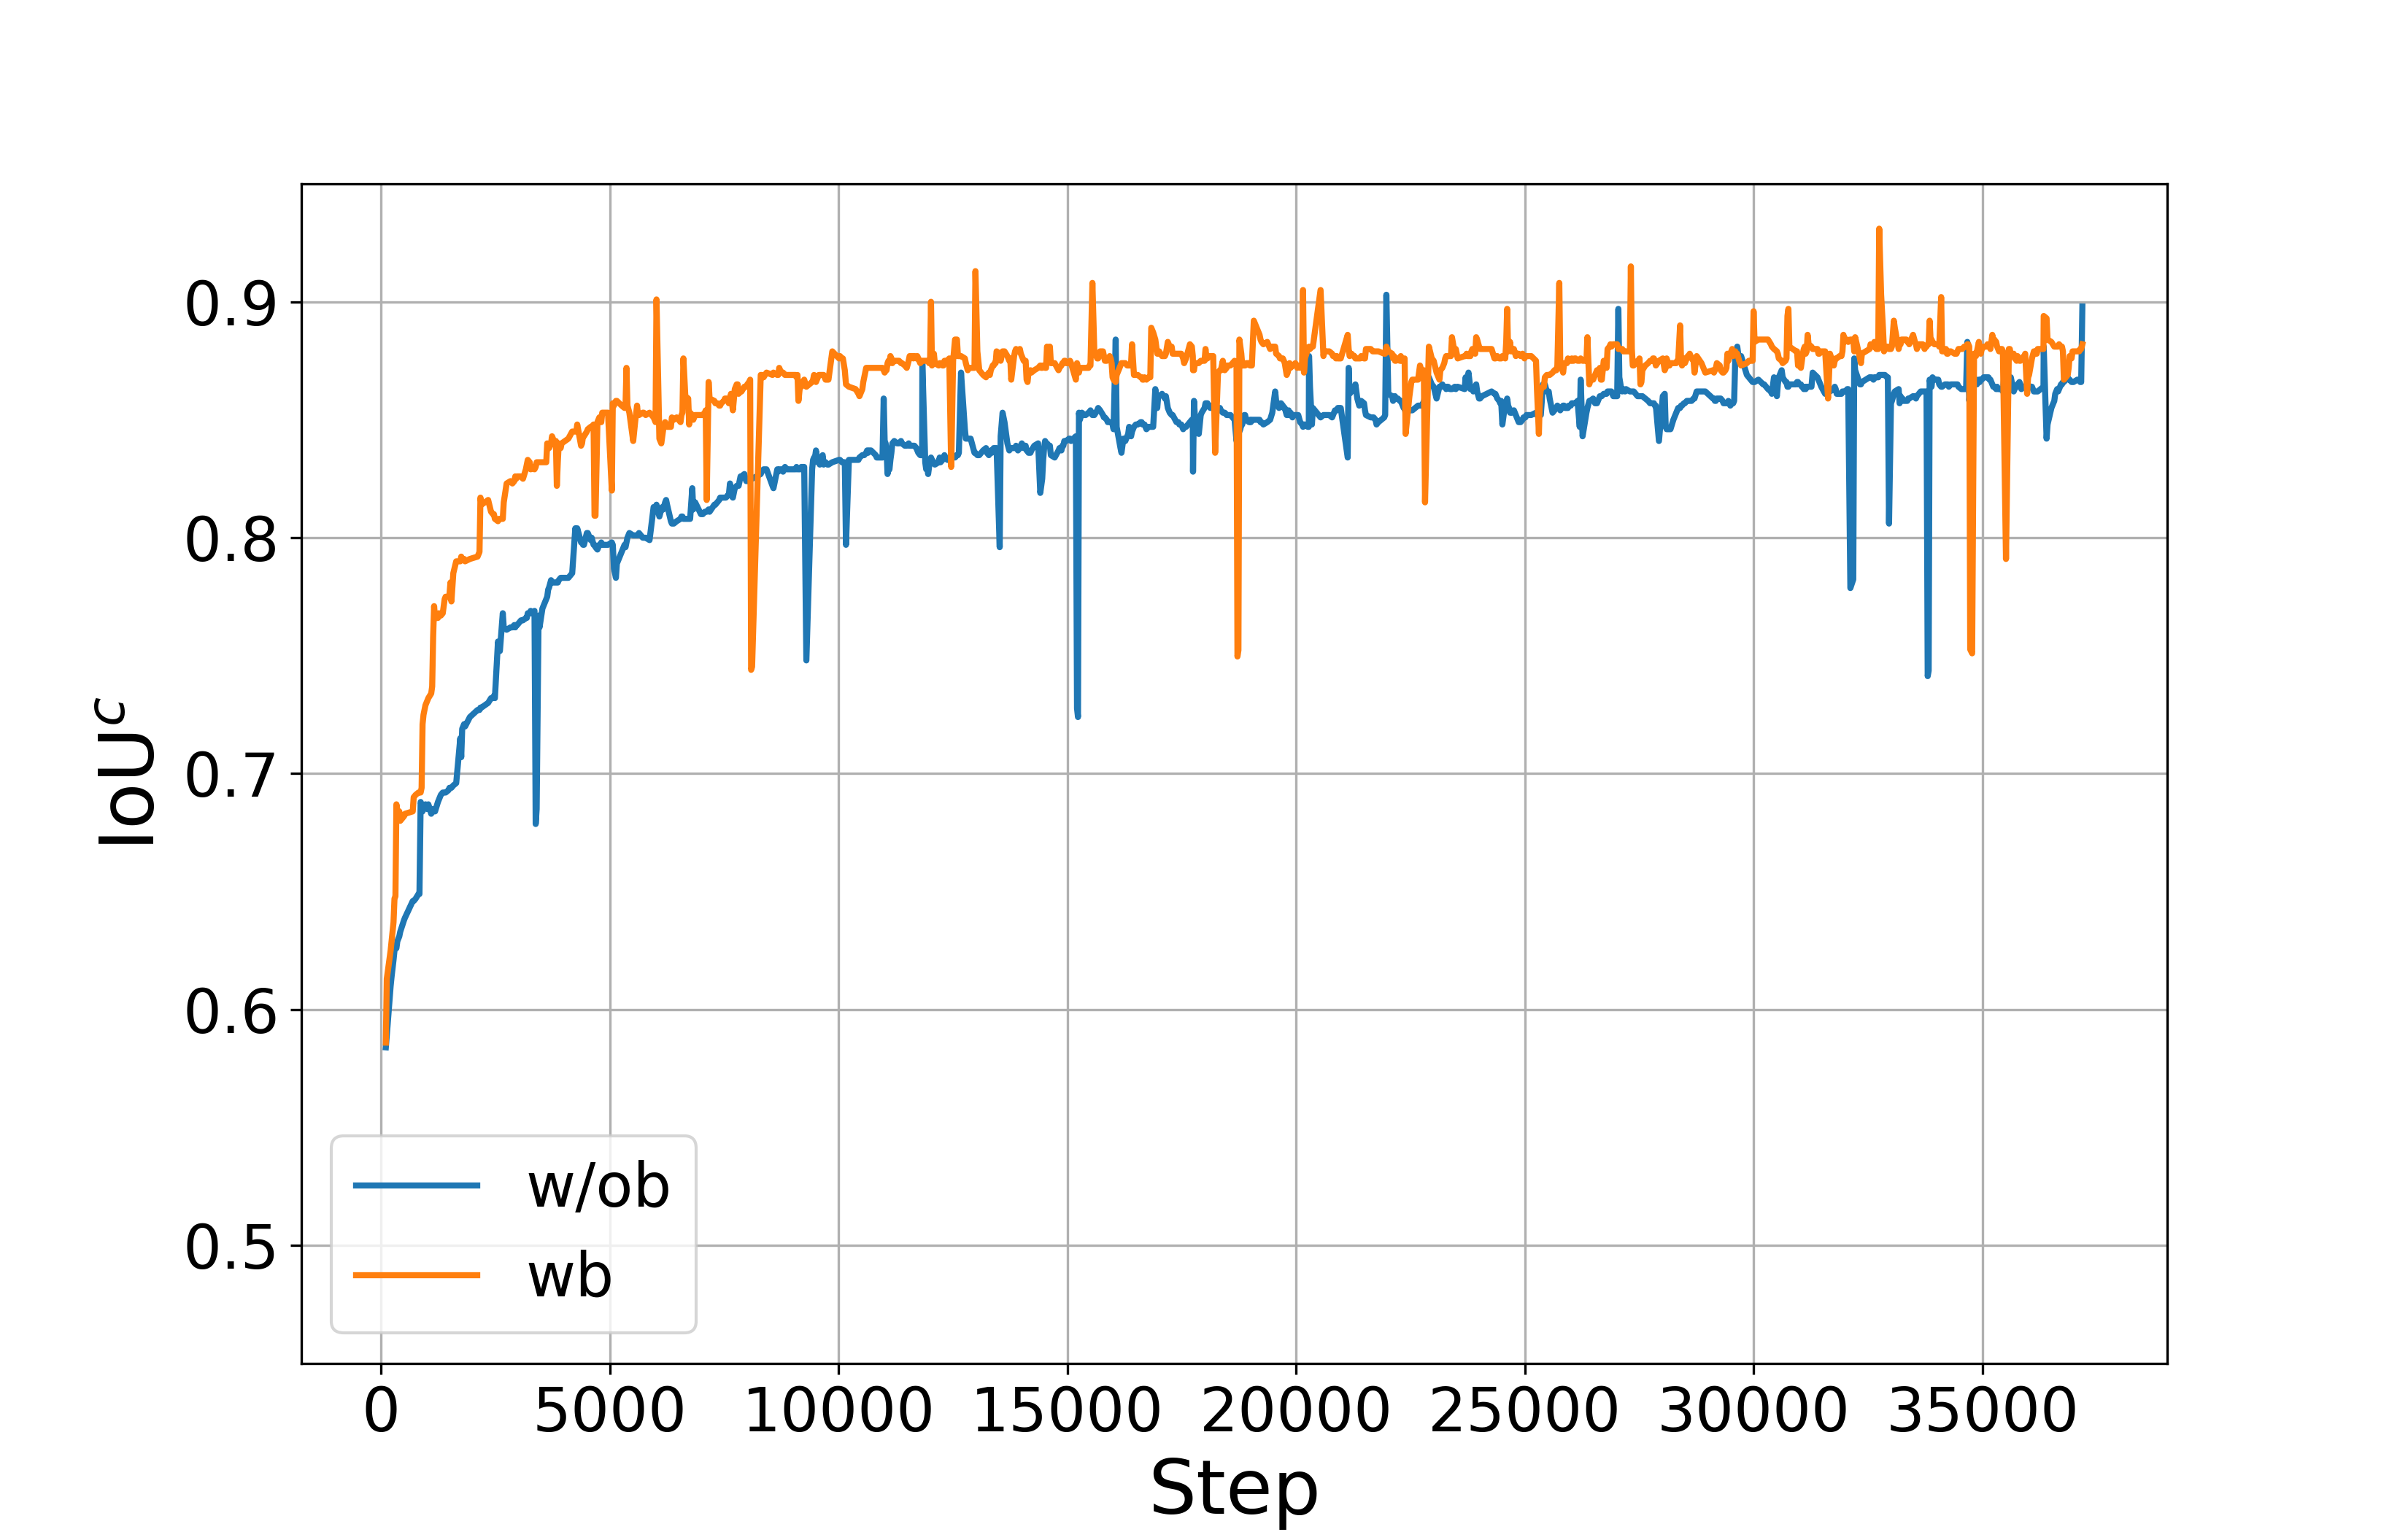
\includegraphics[scale=0.35]{images/AdAwob_unIoU.png}
  \caption{
      类别重平衡对训练中未标记样本生成的伪标签质量的影响
  }
  \label{fig:Adawob_unIOU}
\end{figure}
此外,我们对训练过程中生成的伪标签进行了存储,图\ref{fig:Adawob_unIOU}展示了在整个训练过程中,伪标签评估指标中是否进行类别重平衡的情况下,伪标签和对应的Ground Truth之间计算的$IoU^c$(注意:这里使用的Ground Truth仅用于计算$IoU^c$,而不涉及训练过程中的任何其他方面)。显然,尽管类别重平衡不直接作用于改进伪标签,但它能够更准确地评估伪标签,从而在后续的自适应训练机制中间接地提高了伪标签质量,使它们更接近真正的标签。
\subsubsection{超参数选择}
无监督损失权重的预热过程对AdaSemiCD在半监督变化检测上的性能有重大影响。因此,我们对控制预热过程的两个超参数($\gamma$ 和 $w_{max}$) 的选择进行了消融实验。如表\ref{tab:AdaPram_ablation}所示,在参数(0.1,10)、(0.1,0.1)和(0.1,1.0)的组合下,我们的方法在LEVIR-CD、WHU-CD、CDD三个数据集上的性能最佳。而且,我们的方法对该超参数敏感,参数选择不当会造成较大的性能差异。这是因为我们的方法同时对标记样本进行监督训练和对未标记样本进行无监督训练。如果不能很好地平衡两者之间的关系,就会导致标记样本的过拟合或未标记样本的过多噪声干扰。我们剩下的所有实验都是在这个超参数设置下进行的,比较方法的超参数与原论文中的最佳设置一致。但总的来说,通过经验积累发现,$\gamma$我们总是设置为0.1,$w_{max}$可以在{0.1,1.0,10.0,30.0}中进行尝试,由于深度学习的黑盒性,单阶段半监督学习中监督和无监督的互相影响因素较多,我们暂时无法得出一组在所有情况下都适用的最优参数。在其余数据集上我们仅进行了轻微的超参调整就取得了可观的实验结果,我们将$w_{max}$分别设置为:LEVIR-CD+:10.0;GZ-CD:5.0;EGY-CD:5.0;HRCUS-CD:1.0;DSIFN-CD:10.0;SYSU-CD:1.0;CL-CD:1.0。
\begin{table*}[!htbp]
  % \renewcommand\arraystretch{1.2}
\centering
% \tiny
\caption{超参数敏感性消融实验结果}
   \resizebox{0.9\textwidth}{!}{
   % \setlength{\tabcolsep}{9pt}
\begin{tabular}{p{10mm}p{20mm}p{10mm}cp{15mm}p{10mm}cp{15mm}p{10mm}cp{15mm}p{10mm}} %
  \toprule
  \multirow{2}{*}{\parbox[c]{.1\linewidth}{$\gamma$}} & \multirow{2}{*}{$w_{max}$} & \multicolumn{2}{c}{LEVIR-CD} & & \multicolumn{2}{c}{WHU-CD} & & \multicolumn{2}{c}{CDD}\\
  \cmidrule{3-4} \cmidrule{6-7} \cmidrule{9-10}
  && {$IoU^c$} & {OA} && {$IoU^c$} & {OA} & & {$IoU^c$} & {OA} \\
  \midrule
  0  & 0 (Sup.Only) &   66.8 & 98.13 && %LEVIR-CD
                  55.7 & 97.53 && %WHU-CD
                  67.9 & 95.46 \\  %CDD
  0.05  & 1.0 &   67.2 & 98.17 && %5
                  53.8 & 97.02 && %WHU-CD
                  74.4 & 96.35 \\  %CDD
    0.1   & 1.0   &   71.8 & 98.32 && %LEVIR-CD
                  61.0 & 98.10 && %WHU-CD
                  \underline{\textbf{77.3}} & \underline{\textbf{96.89}} \\  %CDD
      0.3   & 1.0   &   69.9 & 98.26 && %LEVIR-CD
                  59.4 & 98.03 && %WHU-CD
                  76.2 & 96.56 \\  %CDD
      0.5   & 1.0   &  68.7 & 98.15 && %LEVIR-CD
                60.9 & 98.25 && %WHU-CD
                  76.3 & 96.58 \\  %CDD
  1.0   & 1.0   &   67.3 & 98.13 && %LEVIR-CD
                  60.5 & 98.18 && %10
                  72.3 & 95.98 \\ %40
      0.1   & 0.1   &   65.2 & 97.60 && %LEVIR-CD
                  \underline{\textbf{70.8}} & \underline{\textbf{98.70}} && %WHU-CD
                  71.6 & 95.77 \\  %CDD
      0.1   & 0.5   &   68.3 & 98.14 && %LEVIR-CD
                  66.9 & 98.54 && %WHU-CD
                  75.8 & 96.67 \\  %CDD
      0.1   & 5.0   &   73.9 & 98.75 && %LEVIR-CD
                  60.1 & 98.00 && %WHU-CD
                  69.1 & 95.51 \\  %CDD
      0.1   & 10.0   & \underline{\textbf{79.4}} & \underline{\textbf{98.87}} && %LEVIR-CD
                  52.4 & 97.40 && %WHU-CD
                  68.2 & 95.50 \\  %CDD
      0.1   & 30.0   &   71.9 & 98.42 && %LEVIR-CD
                  50.34 & 97.12 && %WHU-CD
                  65.4 & 95.20 \\  %CDD0
  \bottomrule
\end{tabular}
  }
% \normalsize
\label{tab:AdaPram_ablation}
\end{table*}
\subsubsection{计算资源}
虽然引入了额外的自适应机制有效地提高了检测性能,但是一个不可避免的问题就是增加了额外的计算资源消耗,如果耗费了大量的资源而仅仅带来了有限的提升,则得不偿失,因此我们进行了计算资源耗费的实验验证。

实验结果如表\ref{tab:Ada_compute}所示,由于我们对所有实验方法都公平地采用了相同的变化检测网络,因此训练参数数量(46.85M)和计算量(585.85 GFLOPs)都保持相同,我们的AdaSemiCD推理时间方面与其他方法相当。训练时间较长的主要原因是每次训练迭代过程中需要生成和评估两次伪标签,经过统计这一步大约需要0.3s左右,而融合和EMA参数更新分别只需要0.006s和0.03s左右。我们的模型仅仅是前期训练时间增加了25$\%$,但是取得了显著的性能优势,很好地平衡了性能和计算耗费,这对其实际应用具有重要的意义。
\begin{table}[ht]
  \centering
  % \renewcommand\arraystretch{1.2}
  \tiny
  % \caption{Comparison of parameters, computing complexity, training time and inference time of different SSCD methods.}
  \caption{LEVIR-CD数据集上不同方法的参数、计算复杂度和训练时间的比较}
  % 表格标题
  \label{tab:Ada_compute} % 表格标签,用于引用
   \resizebox{0.9\textwidth}{!}{
  \begin{tabular}{p{25mm}p{20mm}p{20mm}p{25mm}p{30mm}p{10mm}} %
  \toprule % 上边框线
  Method & Params(M) & FLOPs(G) & Training Time(s) &Inference Time(ms) &$IoU^c$\\
  \midrule % 中间分割线
  Sup.Only & \hspace{0.3cm}46.85 & \hspace{0.20cm}585.85 & \hspace{1.0cm}77 & \hspace{1.3cm}56 & 61.0\\
  AdvEnt\cite{vu2019advent} & \hspace{0.3cm}46.85 & \hspace{0.20cm}585.85 & \hspace{1.0cm}405 & \hspace{1.3cm}63 & 66.1\\
  s4GAN\cite{mittal2019semi} & \hspace{0.3cm}46.85 & \hspace{0.20cm}585.85 & \hspace{1.0cm}585 & \hspace{1.3cm}58 & 64.0\\
  SemiCDNet\cite{peng2021SemiCDNet} & \hspace{0.3cm}46.85 & \hspace{0.20cm}585.85 & \hspace{1.0cm}408 & \hspace{1.3cm}75 & 67.6\\
  RCR\cite{bandara2022RCR} & \hspace{0.3cm}46.85 & \hspace{0.20cm}585.85 & \hspace{1.0cm}742 & \hspace{1.3cm}59 & 72.5\\
  FPA\cite{Zhang2023FPA} & \hspace{0.3cm}46.85 & \hspace{0.20cm}585.85 & \hspace{1.0cm}727 & \hspace{1.3cm}68 & 73.7\\
  AdaSemiCD & \hspace{0.3cm}46.85 & \hspace{0.20cm}585.85 & \hspace{1.0cm}915 & \hspace{1.3cm}67 &   \textbf{77.7}\\
  \hline
  Oracle & \hspace{0.3cm}46.85 &
  \hspace{0.20cm}585.85 & \hspace{1.0cm}293 & \hspace{1.3cm}55 & 77.9 \\
  \bottomrule % 下边框线
\end{tabular}
}
\end{table}

\begin{figure}[!htbp]
  \centering
  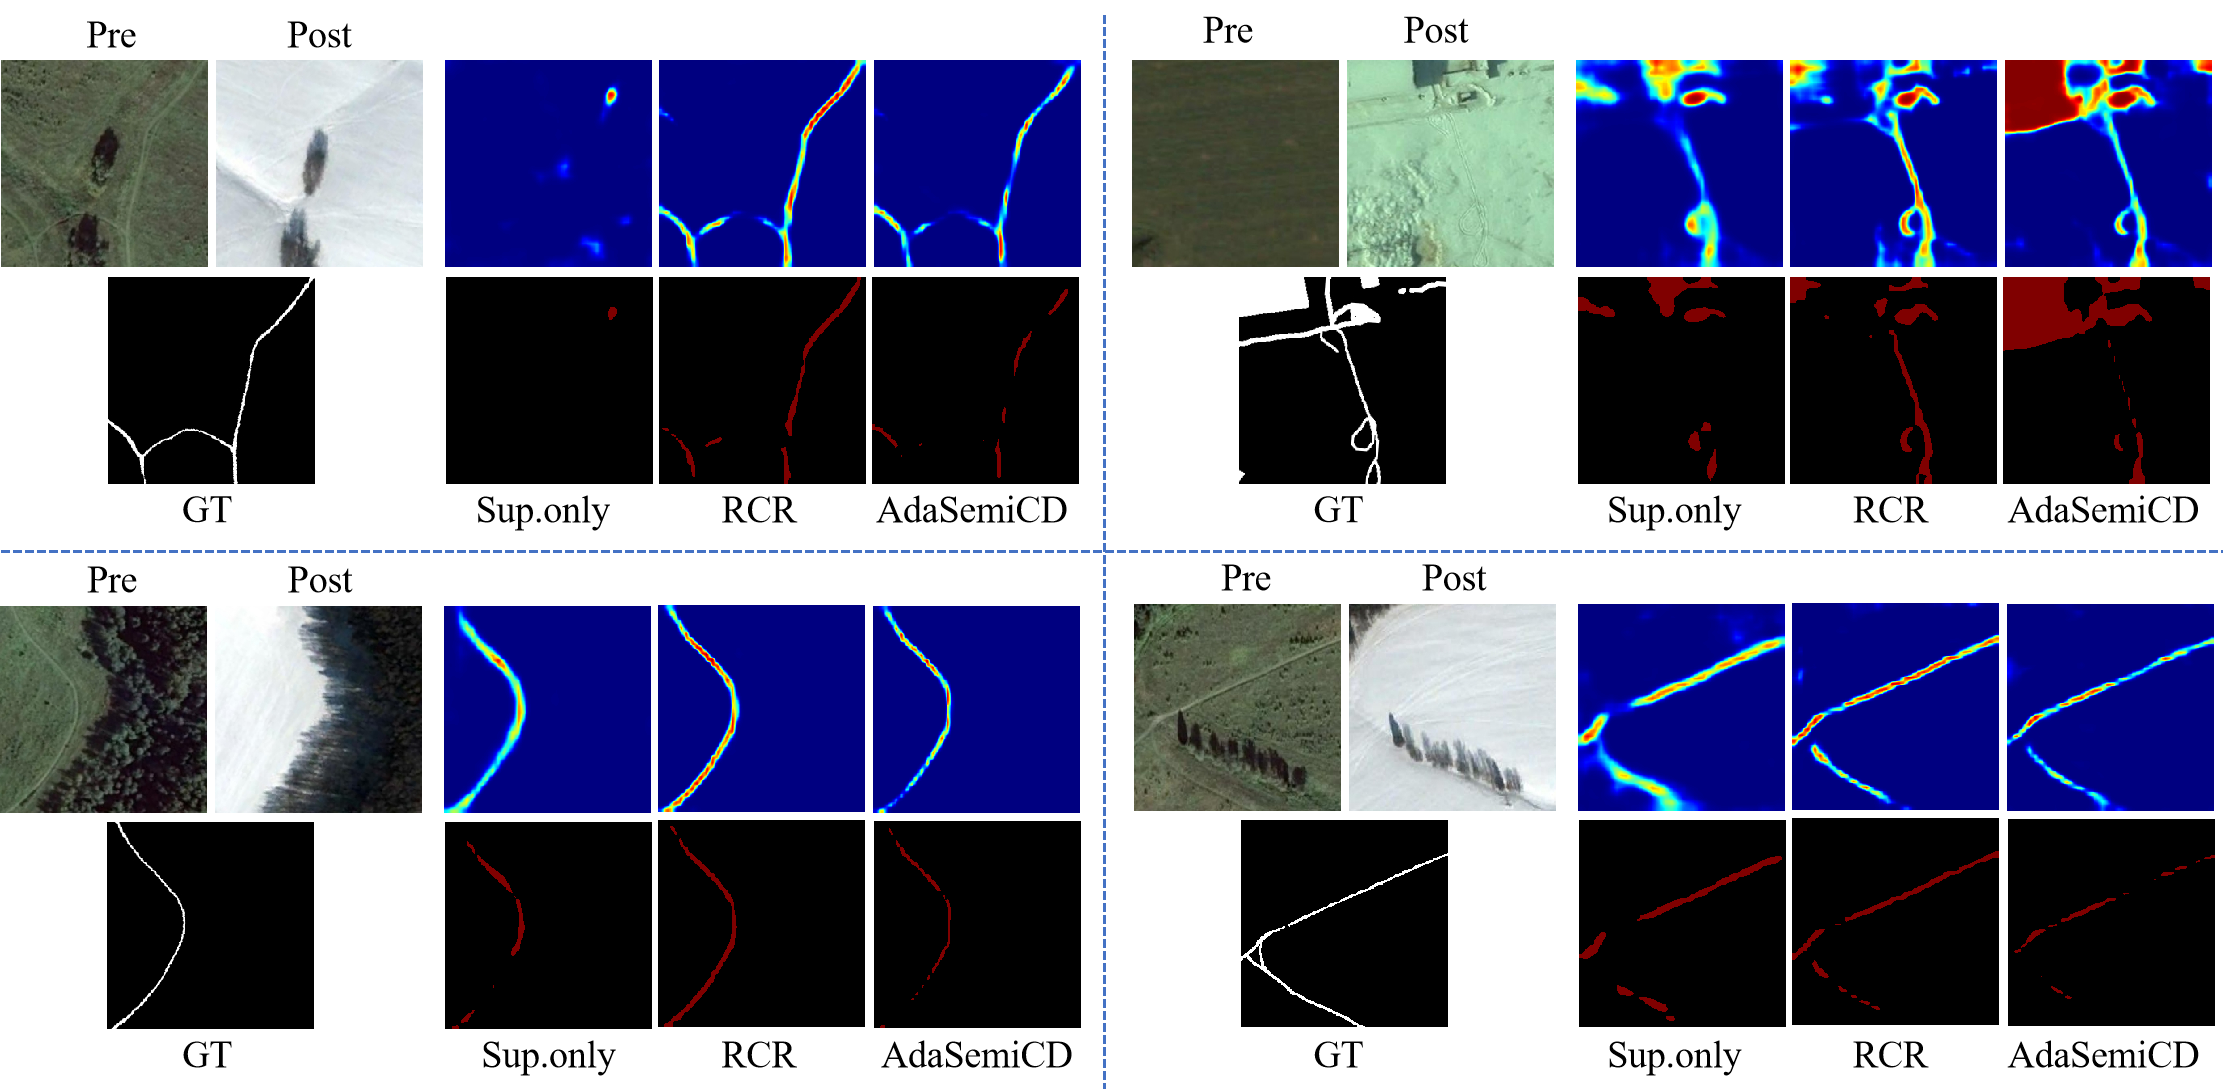
\includegraphics[scale=0.4]{images/AdAerrorVis.png}
  \caption{
    AdASemiCD的一些失效场景
  }
  \label{fig:AdaError}
\end{figure}

\subsection{局限性分析}
虽然我们的方法在大多数情况下都是非常有效的,但我们在实验中也发现在一些特殊场景下依然存在一定的局限性。如图\ref{fig:AdaError}所示,在检测一些细长状变化区域时,我们的方法表现比较挣扎,甚至相比监督基线表现更差。而在识别和检测块状变化区域方面具有很大的优势,如图中右上角的例子所示。这是因为当我们的AdaFusion进行样本融合时,它是patch到patch的融合,很容易截断图像中这种细长状变化的区域,而这种变化类型带有标注的真实训练数据太少,导致没有有效的知识可供学习。

因此,或许更有针对性的融合方法可以避免这种信息丢失。例如,将变化区域视为一个实例,在实例级别进行样本融合。这样,在去除噪声、引入额外的监督信息、扩大样本多样性的同时,可以在很大程度上保留不同变化类型的特征。
\section{本章小结}
本章提出了基于伪标签评估的自适应半监督变化检测算法,首先介绍了基于平均教师模型的整体半监督变化检测框架,包括监督训练、基于一致性正则化的无监督训练两个部分,介绍了总体的损失函数。具体来说,我们对教师模型对未标记训练样本生成的伪标签质量进行评估,并根据评估结果对样本进行自适应的融合,提出了AdaFusion模块,以及对模型参数更新进行自适应的选择,提出了AdaEMA模块,最终提出了AdaSemiCD自适应半监督框架。随后我们介绍了统一的实验设置,与其他几种方法进行了对比实验,从定量和定性两个维度证明了AdaSemiCD的先进性,并设计消融实验验证了各个自适应模块的有效性以及我们的方法中超参数的最优选择。最后从性能和计算开销方面进行了实验探究,我们的方法仅增加了微弱的训练时间开销,而取得了性能上的巨大提升,证明我们的方法是具有实际应用意义的。


\chapter{基于自适应扰动的半监督变化检测算法}
\section{引言}
在此前的的研究中,半监督变化检测领域的最佳方法是基于一致性正则化+自训练的整体方法,它假设对未标记的图像进行准确的预测,使得扰动不会将图像特征推到真实(隐藏)分类决策边界的错误侧。但是其中存在的两个关键问题就是:(1)模型对未标记图像的预测并不总是足够准确的;(2)对无标记图像施加的扰动并不总是对模型训练有效的。

针对问题一,我们在第四章的工作从样本融合方面入手,一定程度地排除了错误伪标签。但这种基于图像块融合的方法还是产生了一些不可避免的问题,即丢失掉了一些变化类型(例如河流、公路)的特征,使得模型在这些类型上的检测效果不佳。我们考虑采用更加准确的融合方式,例如实例级融合,然而这还涉及额外的双时相图像实例分割以及相应的边缘平滑处理运算,这会导致计算资源的耗费成倍数增加。于是我们从RCR\cite{bandara2022RCR}以及经典的半监督分类算法FixMatch\cite{sohn2020fixmatch}中受到启发,采用模型在图像及其扰动版本下的预测概率分布差异作为一致性约束,而不使用单一硬标签作为训练指导,从而减轻错误预测的影响。

半监督学习中的数据扰动主要作用于使得模型在相同的输入上产生预测不一致,从而扩充模型学习从一张样本上能够学习到的特征空间,但是这种扰动没有恒定和具体的目标,能确定的仅有预先定义的离散搜索空间,造成的影响就是有可能造成过大的确认偏差,即在扰动前后模型对其预测概率分布差异较大时进行强行拉近,这反而会破坏模型的泛化性,进而学习到无关或错误的信息,特别是在模型的预测置信度较低的情况下。因此针对问题二,对特征扰动进行精确的调整以更好地适应半监督训练是有必要的。最终我们提出了AdPSemiCD(Semi-supervised change detection algorithm based on sample level adaptive feature perturbation),我们的基本思想是:对模型在无标记样本上的预测进行评估,基于评估结果为每个样本生成一个受限制的特定离散扰动范围,包括特征扰动的数量以及每种扰动的扰动强度。从而在实现一定程度的可控随机性扰动,减少模型的确认偏差,并且提供更加有效的一致性约束,提高模型的泛化性能。

本章介绍了基于自适应特征扰动的半监督变化检测算法——AdPSemiCD,首先从全局角度阐述了算法的框架和流程,随后具体地介绍了我们设计的基于无标记样本预测评估的自适应特征扰动方法。最后在实验部分报告了我们在十个公开数据集上对本章方法进行实验验证取得的实验结果,包括定量实验指标和定性可视分析,此外还对本章提出的自适应扰动模块进行了消融分析,证明了本章研究的有效性。
\section{基于自适应扰动的半监督变化检测框架}
\subsection{整体框架}
与第三章和第四章的研究相同,本章的研究仍然建立在平均教师模型这种简单的半监督学习框架之上,虽然简单但是有效,整体框架如图\ref{fig:AdPFrame}所示。
\begin{figure}[htb]
  \centering
  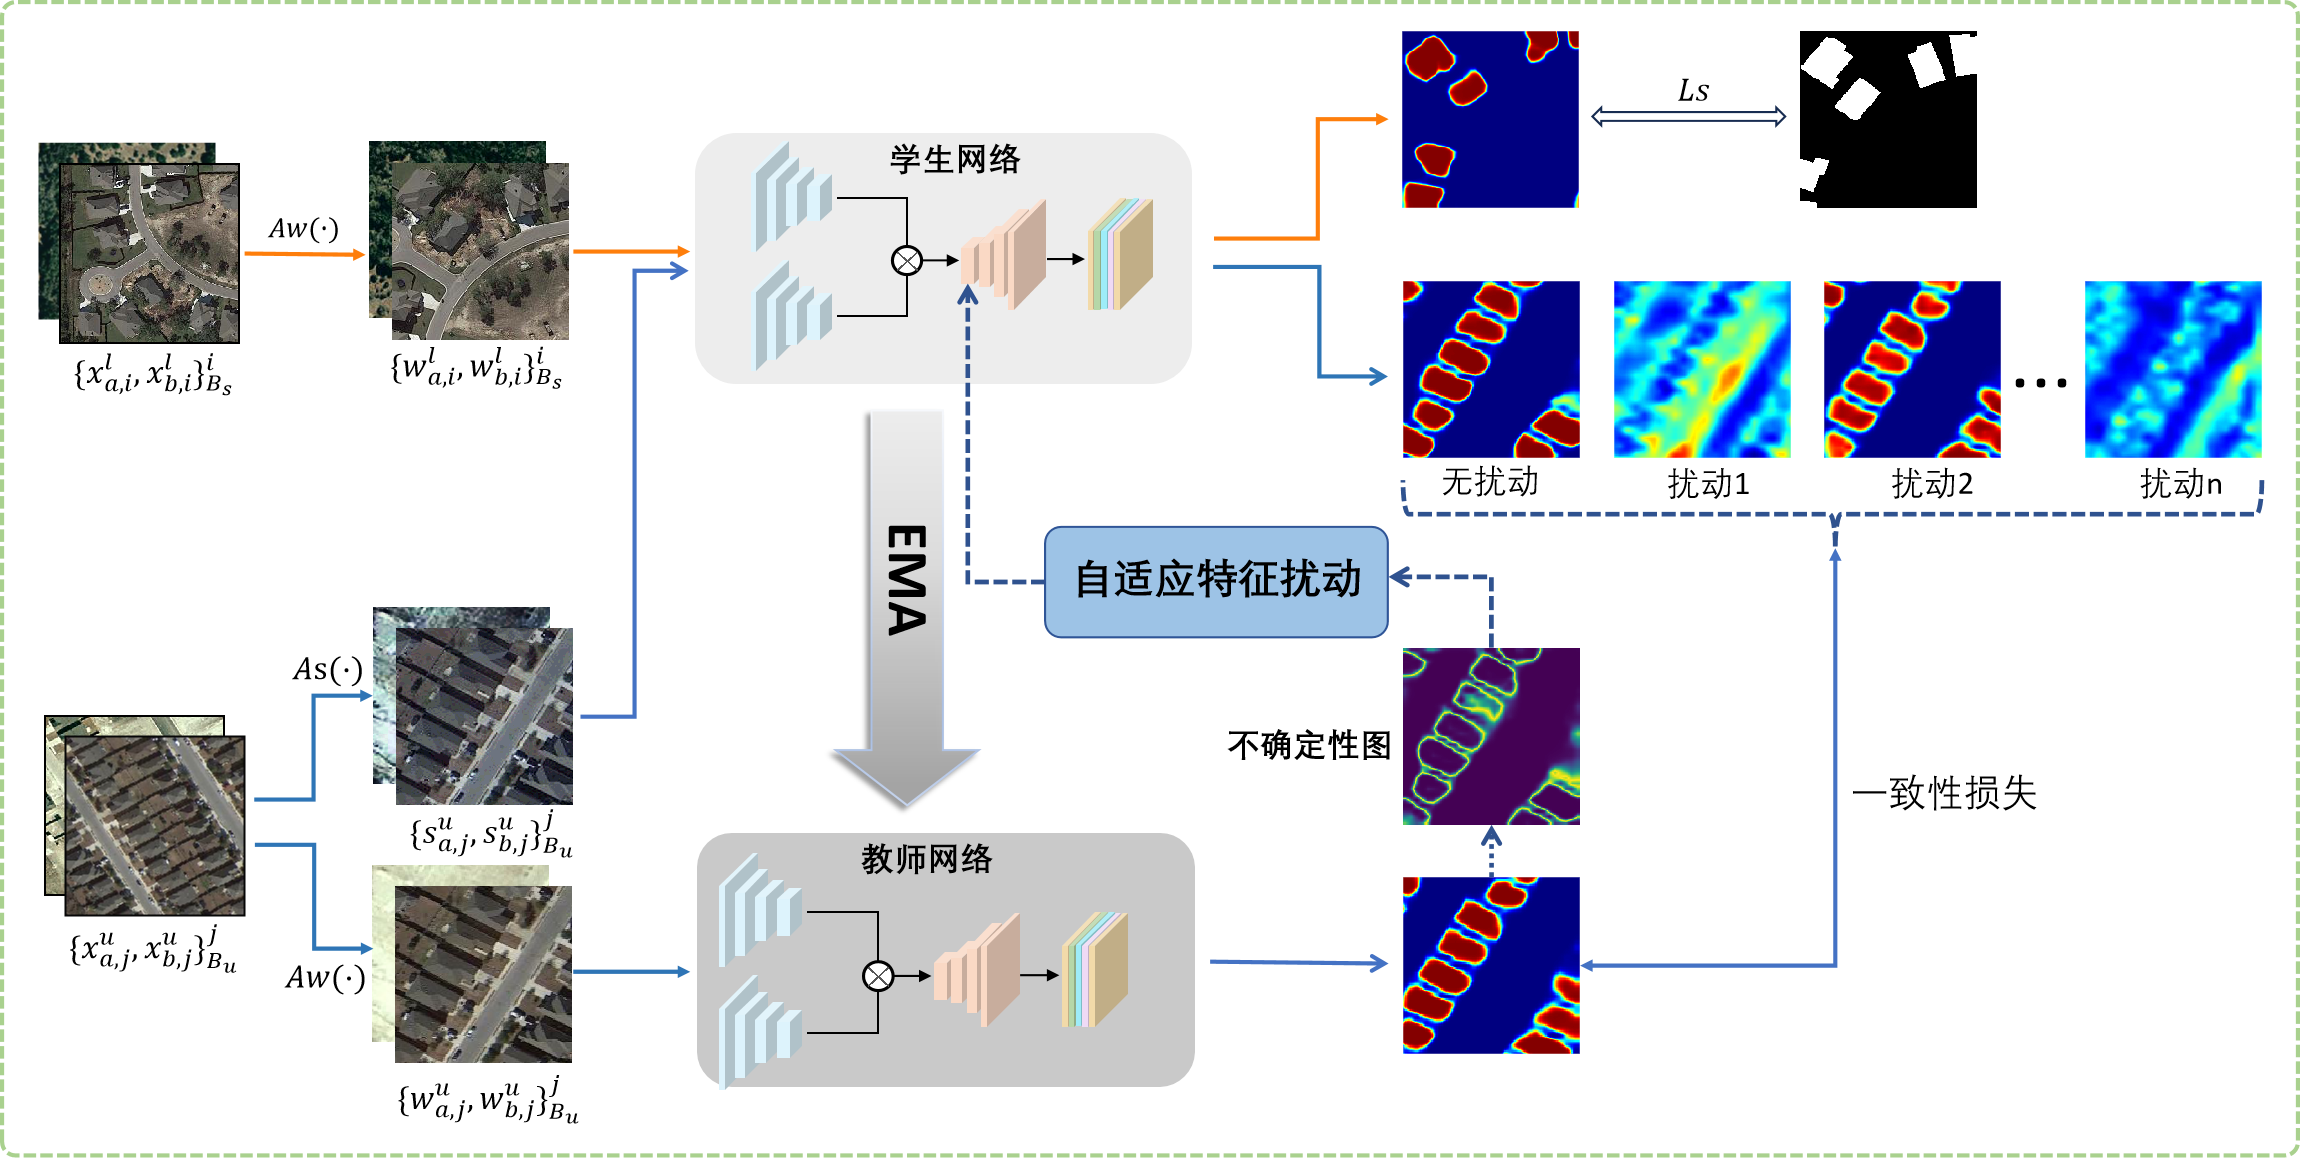
\includegraphics[scale=0.4]{images/AdPFrame.png}
  \caption{
      AdPSemiCD算法的整体框架
  }
  \label{fig:AdPFrame}
\end{figure}

该框架由学生模型和教师模型组成,分别由$\theta_{s}$和$\theta_{t}$进行参数化。具体地说,教师模型能够对无标记图像对进行预测并对其进行评估,教师模型的参数权重通过学生模型权重的指数移动平均来平滑地进行更新,公式表示如下:
\begin{equation}
  \label{eq:AdPema}
  \theta_{t} = \beta \theta_{t}+(1-\beta) \theta_{s}
\end{equation}

其中,$\beta$是常用的动量参数,在本章方法中默认设置为0.996。

另外,在每次训练迭代中,给定一批标记样本$B_{l}=\left\{\left\{x_{a, i}^{l}, x_{b, i}^{l}\right\}, y_{i}^{l}\right\}_{i=1}^{|B_l|}$和一批未标记样本$B_{u}=\left\{x_{a, i}^{u}, x_{b, i}^{u}\right\}_{i=1}^{|B_u|}$,$|B_u|$和$|B_u|$分别是标记样本批次和无标记样本批次的样本数量。我们的训练目标是同时最小化有监督损失$\mathcal{L}_s$和无监督一致性损失$\mathcal{L}_u$来训练学生模型。因此,学生模型的总训练损失是:
\begin{equation}
  \label{eq:AdPLoss}
  \mathcal{L}=\mathcal{L}_{s}+\lambda_{u} \mathcal{L}_{u}
\end{equation}

其中$\lambda_{u}$为无监督损失的权重,在本章中采取与第四章相同的预热函数作为动态调整方案。与大多数图像分割算法相同,我们选择标准的交叉熵损失作为监督训练损失,其计算如下:
\begin{equation}
  \label{eq:AdPLoss_s}
  \mathcal{L}_{s}=\frac{1}{\left|\mathcal{B}_{l}\right|} \sum_{i=1}^{\left|\mathcal{B}_{l}\right|} \mathcal{L}_{ce}\left(M(\theta_s,(x_{a,i}^l,x_{b,i}^l)), y_{i}^{l}\right)
\end{equation}

这里的$y_{i}$和$\hat{y}_{i}$分别表示真实二值标签和模型预测概率。

对于无监督损失,我们需要的是衡量模型在特征扰动前后预测的相似性。因此选择均方误差(Mean Squared Error, MSE),它的核心思想是计算预测值与真实值之间的平方差的平均值,其计算如下:
\begin{equation}
  \label{eq:AdPLoss_mse}
  \mathcal{L}_{MSE}=\frac{1}{\left|\mathcal{B}_{u}\right|} \sum_{i=1}^{\left|\mathcal{B}_{u}\right|}\left(y_{i}-\hat{y}_{i}\right)^{2}
\end{equation}

其中$y_{i}$和$\hat{y}_{i}$分别表示无特征扰动和施加特征扰动之后的模型预测概率,其具体定义我们将在下一小节给出。

最后,对于正则化常数$\lambda_{u}$,我们采用和第四章相同的预热函数,该权重随着训练进程从初始权值0不断增大直至达到预定的最大权重。
\subsection{自适应特征扰动}
在现有的大多数半监督学习研究中,无论是在分类任务中还是在分割任务中,各种扰动技术得到了广泛应用。在半监督学习中,数据扰动的目标是从同一幅图像生成两个不同的视图,其中不需要特定的最优增强策略。此外,正如文献\cite{yuan2021simple}中所讨论的,过度失真的扰动会损害数据分布,降低半监督学习的效果。因此对于每个训练样本,我们应该限定一个扰动空间的范围,以达到最佳的效果。为此,我们设计了一种基于评估无标记样本预测结果的自适应特征扰动方法。

首先我们继续沿用在第四章中设计的伪标签评估指标,对模型在无标记样本上的预测结果进行评估,但不同之处在于我们为了方便利用此评估计算自适应扰动的扰动数量和扰动强度,我们对第四章中的评估指标进行了逆变换,即计算所得从不确定性图变为了确定性图,计算公式如下:
\begin{equation}
  \label{eq:certainty}
  C\left(y_{i}\right)=D\left(y_{i}\right) \cdot E^{\prime}\left(y_{i}\right)
\end{equation}
其中$y_{i}$表示教师模型在无标记样本上的预测概率,此外$D(\cdot)$和$E^{\prime}(\cdot)$计算公式如\ref{eq:entropy}、\ref{eq:balance}以及\ref{eq:abs}。

接下来对整个无标记样本批次内的样本确定性图$\{ C_j \}_{j=1}^{|\mathcal{B}_u|}$进行归一化得到$\{C_j^{\prime} \}_{j=1}^{|\mathcal{B}_u|}$,在此我们使用最大归一化,公式如下:
\begin{equation}
  \label{eq:normalC}
  C_j^{\prime}=\frac{C_j-C_{\min }}{C_{\max }-C_{\min }}
\end{equation}

其中$C_j^{\prime} \in [0,1]$,接下来将其作为一个缩放因子,来计算得到每对样本的特征扰动数量,如公式\ref{eq:numpfperturb},其中$Num$表示扰动池中的扰动方法总数。最后从扰动池中为该样本随机抽取相应数量的扰动方法作用于其在学生模型上融合后的高维特征。
\begin{equation}
  \label{eq:numpfperturb}
  num_j=C_j^{\prime} \times Num
\end{equation}
其中扰动池包含以下七种特征扰动,扰动名称、扰动方式以及主要参数和其预定义取值范围见表\ref{tab:feature_perturb}。
\begin{table}[h!]
  \centering
  \caption{AdPSemiCD使用的特征扰动方法}
  \begin{tabular}{@{}lp{8cm}l@{}}
  \toprule
  \textbf{扰动名称} & \textbf{作用描述} & \textbf{主要参数}\\ \midrule
  无扰动 & 保留原始特征 & ——\\
  特征加噪声 & 添加噪声,干扰特征表示 & $uniform_{range} \in [0, 1.0]$\\
  特征丢弃 & 丢弃部分特征 & $ threshold \in [0, 1.0]$\\
  特征裁剪 & 仅保留一定范围内的特征 & $ threshold \in [0, 1.0]$\\
  引导特征遮挡 & 遮挡部分背景特征区域 & $ erase \in [0, 1.0]$ \\
  特征模糊 & 通过平滑操作使特征值分布更加均匀 & $ \sigma \in [0.5, 2.0]$ \\
  通道扰动 & 不同通道的特征进行互换 & $ num \in [10, 50]$ \\
  对抗扰动 & 对部分区域特征施加对抗扰动 & $ \epsilon \in [1.0, 5.0]$ \\
  \bottomrule
  \end{tabular}
  \label{tab:feature_perturb}
\end{table}

对于选中的扰动,我们同样使用归一化后的确定性作为缩放因子,为每对样本计算所选取扰动的参数,来自适应地控制扰动的强度。计算公式如下:
\begin{equation}
  \label{eq:parmpfperturb}
  \theta_j^i=C_j^{\prime} \times \theta^i
\end{equation}

$\left \{{\theta^i}\right \}_{i=1}^{Num}$即所有扰动的预定义参数集合,如表\ref{tab:feature_perturb}中所列举。

最后,将每对样本自适应选择的扰动施加到相应样本经过学生模型编码器和特征差异模块之后的融合特征值上,扰动后的特征再经过解码器进行上采样从而输出为扰动版本的预测概率。假设经过编码器和特征差异模块之后的图像特征为${\mathcal{F}}_{s,j}$,则扰动过程可表示为:
\begin{equation}
  \label{eq:perturb-process}
  {\hat{\mathcal{F}}}_{s,j} = {\mathcal{F}}_{s,j} \oplus {\mathcal{P}}_i(\theta^i)
\end{equation}

得到$num_j$个扰动特征$ \left \{(\hat{\mathcal{F}}_{s,j})_n\right \}_{n=1}^{num_j}$,再分别输入解码器中得到$num_i$个扰动预测概率$ \left \{(\hat{p}_{s,j})_n\right \}_{n=1}^{num_j}$,
\begin{equation}
  \label{eq:perturb-decode}
  \hat{p}_{s,j}={f_d}(\hat{\mathcal{F}}_{s,j})
\end{equation}

当然此外还有一个无扰动版本的学生模型输出,即$p_{s,j}=f_d(\mathcal{F}_{s,j})$。于是,在一致性约束之下,我们在无标记样本上的无监督训练目标就是拉近这些扰动版本输出和无扰动版本输出已经教师模型在弱增强样本上的输出之间的距离,最小化输出概率分布之间的差异。无监督损失计算如下:
\begin{equation}
  \label{eq:AdPLoss_u}
  \mathcal{L}_{\text {u}}= \frac{1}{\left|\mathcal{B}_{u}\right|}\sum_{j=1}^{|\mathcal{B}_u |}\left(\sum_{i=1}^{num_{j}} \mathcal{L}_{MSE}\left(\left(\hat{p}_{s,j}\right)_{i}, p_{w,j}\right)+ \\
  \mathcal{L}_{MSE}\left(\left(p_{s,j}\right)_{i}, p_{w,j}\right)\right)
\end{equation}
\section{实验结果及分析}
\subsection{实验设置}
本章所有实验数据集划分以及共同的实现细节部分均与第四章保持一致。
\subsection{对比实验}
为了验证本章提出的AdPSemiCD的有效性,与第四章类似,我们在十个数据集上与三种半监督变化检测算法与两种半监督语义分割算法进行了全方位的对比实验,包括实验指标对比和可视化结果对比。
\begin{figure}[H]
  \centering
  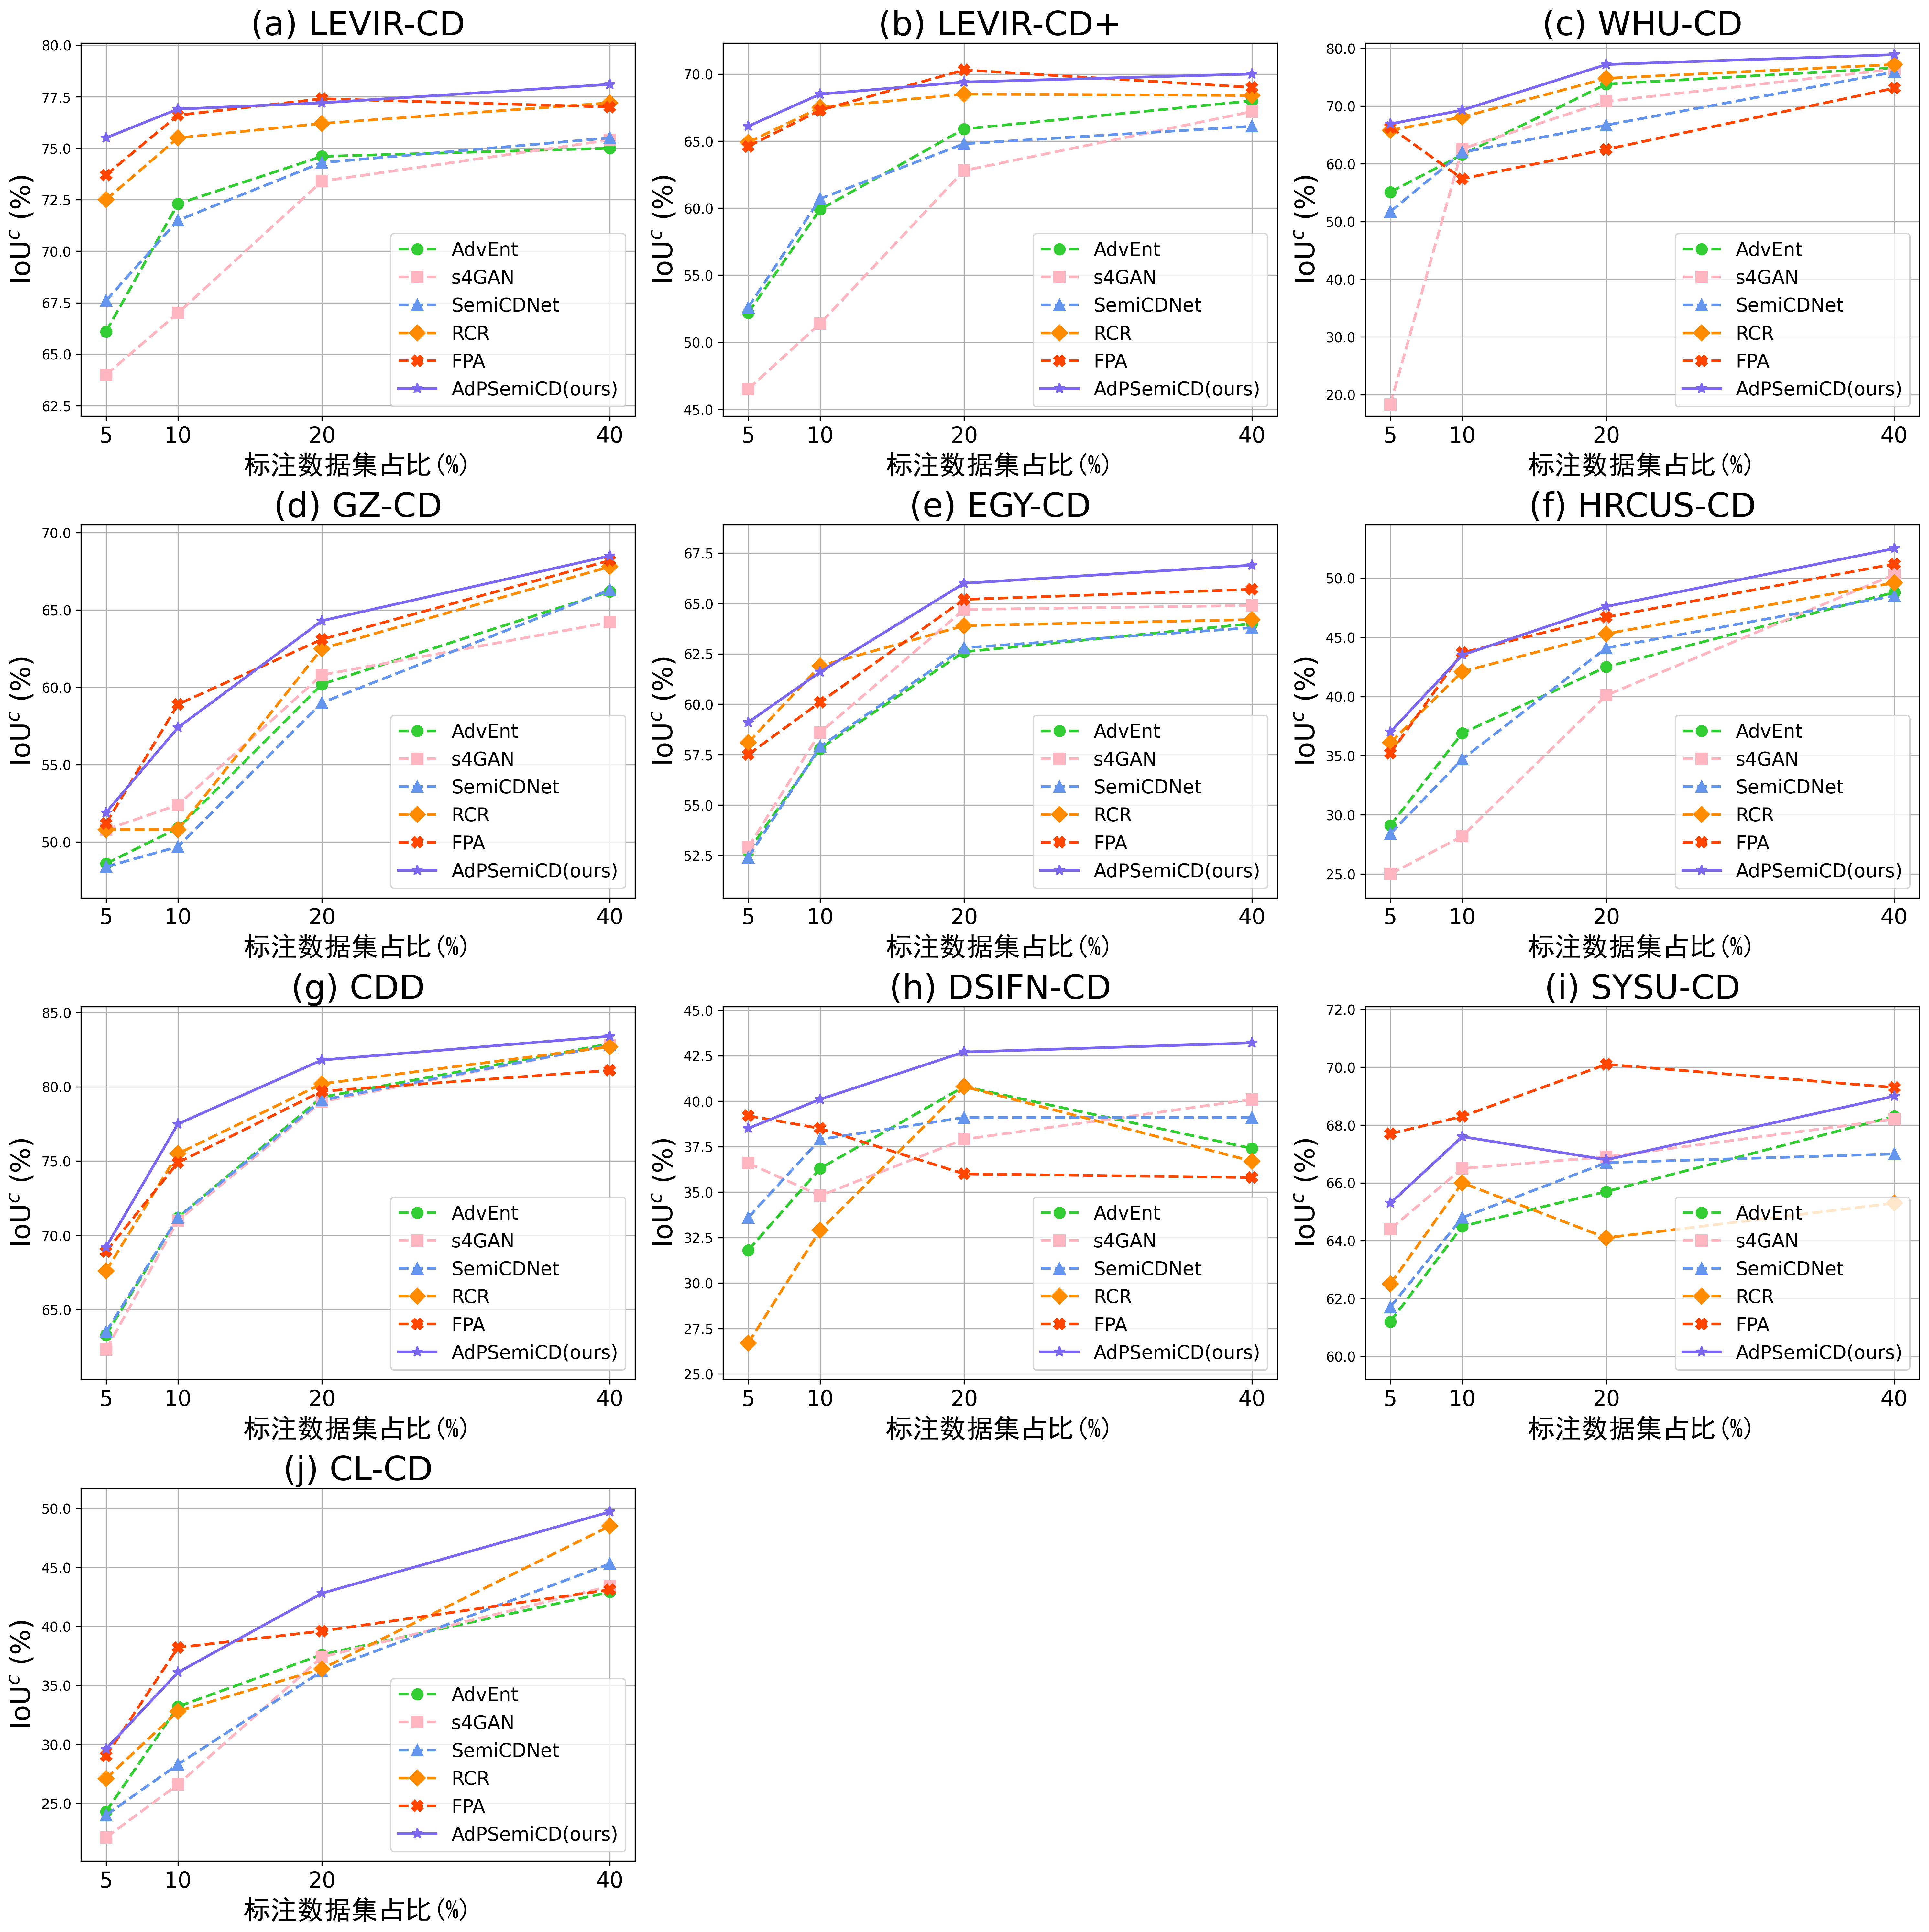
\includegraphics[scale=0.30]{images/AdPvis_plot.png}
  \caption{
    AdPSemiCD与SOTA方法在10个数据集上的性能对比折线图
  }
  \label{fig:AdPiou_plot}
\end{figure}
\subsubsection{定量对比}
我们在所有10个数据集上进行了实验,表\ref{tab:AdP-building}和表\ref{tab:AdP-mutil}分别报告了我们在建筑物变化检测数据集和多类变化检测数据集上的实验结果。其中,Oracle是在整个训练数据集上进行全监督训练的结果。另外图\ref{fig:AdPiou_plot}更直观地展示了我们的所有实验定量结果。值得注意的是,我们的方法在所有数据集的几乎所有半监督划分设置中都实现了最先进的性能。在大多数情况下,所有的半监督变化检测方法在相应的划分设置下都比仅监督的基线方法表现得更好,这证明了半监督方法在从大量未标记的训练样本中学习到了更多的知识。

如表\ref{tab:AdP-building}所示,其中蓝色高亮部分代表着最优结果,下划线标注的是次优结果。我们所提出的AdPSemiCD框架在几乎所有建筑物变化检测数据集上都达到了最佳的效果,并且在所有数据集上表现都比RCR更好,这说明我们的自适应特征扰动一致性比RCR中采用的随机特征扰动一致性更加适合半监督变化检测。

\textbf{建筑物变化检测}:
\begin{table}[!htbp]
  \centering
  % \tiny
  \scriptsize
  \caption{不同CD方法在建筑物变化检测数据集上的定量性能对比}
  \resizebox{0.9\textwidth}{!}{
  \begin{tabular}{p{20mm}p{25mm}p{8mm}p{8mm}cp{8mm}p{8mm}cp{8mm}p{8mm}cp{8mm}p{8mm}} %
      \toprule
      \multirow{2}{*}{数据集} & \multirow{2}{*}{方法} & \multicolumn{2}{c}{5\%} & & \multicolumn{2}{c}{10\%} & & \multicolumn{2}{c}{20\%} & & \multicolumn{2}{c}{40\%}\\
      \cmidrule{3-4} \cmidrule{6-7} \cmidrule{9-10} \cmidrule{12-13}
      & & {$IoU^c$} & {OA} && {$IoU^c$} & {OA} & & {$IoU^c$} & {OA} &&{$IoU^c$} & {OA}\\
      \midrule
      \multirow{8}{*}{LEVIR-CD}
      & 仅监督   &   61.0 & 97.60 && 66.8 & 98.13 && 72.3 & 98.44 && 74.9 & 98.60 \\ %40
      & AdvEnt\cite{vu2019advent}& 66.1 & 98.08 && 72.3 & 98.45 && 74.6 & 98.58 && 75.0 & 98.60 \\ %40
      & s4GAN\cite{mittal2019semi}& 64.0 & 97.89 && 67.0 & 98.11 && 73.4 & 98.51 && 75.4 & 98.62 \\
      & SemiCDNet\cite{peng2021SemiCDNet} & 67.6 & 98.17 && 71.5 & 98.42 && 74.3 & 98.58 && 75.5 & 98.63 \\ %40
      & RCR\cite{bandara2022RCR}& 72.5 & 98.47 && 75.5 & 98.63 && 76.2 & 98.68 && \underline{77.2} & 98.72 \\
      & FPA\cite{Zhang2023FPA}& \underline{73.7} & \underline{98.57} && \underline{76.6} & \underline{98.72} && \cellcolor{mycyan}\textbf{77.4} & \cellcolor{mycyan}\textbf{98.75} && 77.0 & \underline{98.74} \\
      \rowcolor{mycyan}
      \multirow{-8}{*}{\cellcolor{white}}& \cellcolor{white}AdPSemiCD   &   \textbf{75.5} & \textbf{98.63} && \textbf{76.9} & \textbf{98.70} && \cellcolor{white}\underline{77.2} & \cellcolor{white}\underline{98.74} && \textbf{78.1}& \textbf{98.80} \\%40
      \cline{2-13}
      & Oracle & \multicolumn{11}{c}{$ IoU^c$=\textcolor{red}{\bf 77.9} and OA=\textcolor{red}{\bf 98.77}} \\
      \bottomrule
      %\midrule
      \multirow{8}{*}{LEVIR-CD+}
      & 仅监督   &   52.0 & 97.72 && 58.4 & 98.06 && 66.1 & 98.31 && 66.2 & 98.42 \\ %40
      & AdvEnt\cite{vu2019advent}& 52.2 & 97.68 && 59.9 & 98.11 && 65.9 & 98.37 && 68.0 & 98.51 \\ %40
      & s4GAN\cite{mittal2019semi}& 46.5 & 97.25 && 51.4 & 97.66 && 62.8 & 98.18 && 67.2 & 98.46 \\
      & SemiCDNet\cite{peng2021SemiCDNet} & 52.6 & 97.66 && 60.7 & 98.24 && 64.8 & 98.37 && 66.1 & 98.38 \\ %40
      & RCR\cite{bandara2022RCR}& \underline{64.9} & 98.25 && \underline{67.5} & \underline{98.45} && 68.5 & 98.52 && 68.4 & 98.51 \\
      & FPA\cite{Zhang2023FPA}& 64.6 & \underline{98.30} && 67.3 & 98.40 && \cellcolor{mycyan}\textbf{70.3} & \cellcolor{mycyan}\textbf{98.64} && \underline{69.0} & \underline{98.59} \\
      \rowcolor{mycyan}
      \multirow{-8}{*}{\cellcolor{white}}& \cellcolor{white}AdPSemiCD   &   \textbf{66.1} & \textbf{98.40} && \textbf{68.5} & \textbf{98.49} && \cellcolor{white}\underline{69.4} & \cellcolor{white}\underline{98.58} && \textbf{70.0} & \textbf{98.62} \\%40
      \cline{2-13}
      & Oracle & \multicolumn{11}{c}{$ IoU^c$=\textcolor{red}{\bf 70.5} and OA=\textcolor{red}{\bf 98.63}} \\
      \bottomrule
      % \midrule
      \multirow{8}{*}{WHU-CD}
      & 仅监督   &   50.0 & 97.48 && 55.7 & 97.53 && 65.4 & 98.20 && 76.1 & 98.94 \\ %40
      & AdvEnt\cite{vu2019advent}& 55.1 & 97.90 && 61.6 & 98.11 && 73.8 & 98.80 && 76.6 & 98.94 \\ %40
      & s4GAN\cite{mittal2019semi}& 18.3 & 96.69 && 62.6 & 98.15 && 70.8 & 98.60 && 76.4 & 98.96 \\
      & SemiCDNet\cite{peng2021SemiCDNet} & 51.7 & 97.71 && 62.0 & 98.16 && 66.7 & 98.28 && 75.9 & 98.93 \\ %40
      & RCR\cite{bandara2022RCR}& 65.8 & 98.37 && \underline{68.1} & \underline{98.47} && \underline{74.8} & \underline{98.84} && \underline{77.2} & \underline{98.96} \\
      & FPA\cite{Zhang2023FPA}& \underline{66.3} & \underline{98.45} && 57.4 & 97.69 && 62.5 & 98.48 && 73.1 & 98.69 \\
      \rowcolor{mycyan}
      \multirow{-8}{*}{\cellcolor{white}}& \cellcolor{white}AdPSemiCD   &   \textbf{66.9} & \textbf{98.54} && \textbf{69.3} & \textbf{98.65} && \textbf{77.2} & \textbf{98.94} && \textbf{78.9} & \textbf{99.09} \\%40
      \cline{2-13}
      & Oracle & \multicolumn{11}{c}{$ IoU^c$=\textcolor{red}{\bf 85.5} and OA=\textcolor{red}{\bf 99.38}} \\
      \bottomrule
      % \midrule
      \multirow{8}{*}{GZ-CD}
      & 仅监督   &   47.5 & 93.56 && 51.4 & 94.26 && 58.0 & 95.65 && 66.3 & 96.62 \\ %40
      & AdvEnt\cite{vu2019advent}& 48.6 & 94.39 && 50.9 & 94.89 && 60.2 & 95.79 && 66.2 & 96.58 \\ %40
      & s4GAN\cite{mittal2019semi}& 50.8 & 94.38 && 52.4 & 94.98 && 60.8 & 95.94 && 64.2 & 96.39 \\
      & SemiCDNet\cite{peng2021SemiCDNet} & 48.4 & 93.58 && 49.7 & 94.79 && 59.0 & 95.66 && 66.3 & 96.57 \\ %40
      & RCR\cite{bandara2022RCR}& 50.8 & 93.82 && 50.8 & 94.69 && 62.5 & 96.07 && 67.8 & 96.61 \\
      & FPA\cite{Zhang2023FPA}& \cellcolor{white}51.2 & \cellcolor{white}93.92 && \cellcolor{mycyan}\textbf{58.9} & \cellcolor{mycyan}\textbf{95.78} && \underline{63.1} & \underline{96.26} && \underline{68.2} & \underline{96.82} \\
      \rowcolor{mycyan}
      \multirow{-8}{*}{\cellcolor{white}}& \cellcolor{white}AdPSemiCD   &   \textbf{51.9} & \textbf{94.58} && \cellcolor{white}\underline{57.4} & \cellcolor{white}\underline{95.59} && \textbf{64.3} & \textbf{96.30} && \textbf{68.5} & \textbf{96.88} \\%40
      \cline{2-13}
      & Oracle & \multicolumn{11}{c}{$ IoU^c$=\textcolor{red}{\bf 69.0} and OA=\textcolor{red}{\bf 96.93}} \\
      \bottomrule
      \multirow{8}{*}{EGY-CD}
      & 仅监督   &   49.8 & 95.73 && 54.6 & 96.38 && 61.4 & 96.83 && 65.1 & 97.25 \\ %40
      & AdvEnt\cite{vu2019advent}& 52.7 & 96.01 && 57.8 & 96.58 && 62.6 & 96.86 && 64.0 & 97.19 \\ %40
      & s4GAN\cite{mittal2019semi}& 52.9 & 95.94 && 58.6 & 96.50 && 64.7 & 97.09 && 64.9 & 97.27 \\
      & SemiCDNet\cite{peng2021SemiCDNet} & 52.4 & 96.00 && 57.9 & 96.31 && 62.8 & 96.95 && 63.8 & 97.19 \\ %40
      & RCR\cite{bandara2022RCR}& \underline{58.1} & 96.50 && 59.9 & 96.77 && 63.9 & 97.08 && 64.2 & 97.18 \\

      \multirow{-7}{*}{\cellcolor{white}}& \cellcolor{white}
      FPA\cite{Zhang2023FPA}& 57.5 & \underline{96.52} && \underline{60.1} & \underline{96.86} && \underline{65.2} & \underline{97.25} && \underline{65.7} & \underline{97.34} \\

      \rowcolor{mycyan}
      \multirow{-8}{*}{\cellcolor{white}}& \cellcolor{white}AdPSemiCD   &   \textbf{59.1} & \textbf{96.58} && \textbf{61.6} & \textbf{96.90}  && \textbf{66.0} & \textbf{97.31} && \textbf{66.9} & \textbf{97.37} \\%40
      \cline{2-13}
      & Oracle & \multicolumn{11}{c}{$ IoU^c$=\textcolor{red}{\bf 67.6} and OA=\textcolor{red}{\bf 97.54}} \\
      \bottomrule
      \multirow{8}{*}{HRCUS-CD}
      & 仅监督   &   29.5 & 98.11 && 36.0 & 98.45 && 43.4 & 98.68 && 48.9 & 98.84 \\ %40
      & AdvEnt\cite{vu2019advent}& 29.1 & 98.11 && 36.9 & 98.40 && 42.5 & 98.61 && 48.8 & 98.71 \\ %40
      & s4GAN\cite{mittal2019semi}& 25.0 & 97.86 && 28.2 & 98.24 && 40.1 & 98.62 && 50.3 & \underline{98.85} \\
      & SemiCDNet\cite{peng2021SemiCDNet} & 28.4 & 98.00 && 34.7 & 98.44 && 44.1 & 98.68 && 48.5 & 98.74 \\ %40
      & RCR\cite{bandara2022RCR}& \underline{36.1} & 98.36 && 42.1 & \underline{98.69} && 45.3 & 98.76 && 49.6 & 98.66 \\

      & FPA\cite{Zhang2023FPA}& 35.2 & \underline{98.37} && \cellcolor{mycyan}\textbf{43.7} & 98.65 && \underline{46.7} & \underline{98.82} && \underline{51.2} & 98.81 \\

      \rowcolor{mycyan}
      \multirow{-8}{*}{\cellcolor{white}}& \cellcolor{white}AdPSemiCD   &  \textbf{37.0} & \cellcolor{mycyan}\textbf{98.49} && \cellcolor{white}\underline{43.5} & \textbf{98.72} && \textbf{47.6} & \textbf{98.85} && \textbf{52.5} & \textbf{98.89} \\%40
      \cline{2-13}
      & Oracle & \multicolumn{11}{c}{$ IoU^c$=\textcolor{red}{\bf 59.0} and OA=\textcolor{red}{\bf 99.06}} \\
      \bottomrule
  \end{tabular}
  }
  \label{tab:AdP-building}
\end{table}

具体来说,我们的AdPSemiCD在LEVIR-CD、LEVIR-CD+、WHU-CD、GZ-CD、EGY-CD、HRCUS-CD上分别在四种半监督比例设置下平均提升了0.70、0.58、1.48、0.28、1.1、0.65个百分点的$IoU^c$。此外,值得说明的是,在第四章AdaSemiCD表现不佳的数据集——GZ-CD上,本章提出的AdPSemiCD取得了更好的效果,在三种半监督实验设置下都超越了FPA方法。正如第四章所分析的,这是由于GZ-CD的分辨率最低并且手工标注比较粗糙,对于AdaSemiCD这样基于伪标签自训练的方法提出了巨大的挑战,而本章的方法并不依赖于二值硬伪标签,而是利用一个可控搜索空间内的扰动一致性作为训练约束,克服了伪标签不准确这一困难。但是在其他相对简单的数据集上,本章AdPSemiCD带来的性能提升相比AdaSemiCD就比较有限了,这是由于在伪标签足够可靠的情况下,一致性正则化+自训练的半监督方法普遍比单纯的一致性正则化方法表现更好。

\textbf{多类变化检测}:
如表\ref{tab:AdP-mutil}所示,与建筑物变化检测数据集上的趋势和规律相同,我们的AdPSemiCD虽然同样在几乎所有多类别变化检测数据集和所有半监督比例设置下都实现了最佳性能,并且在所有实验中都超越了RCR,但是总体上带来的提升相比AdaSemiCD更有限。

具体来说,在CDD数据集上,AdPSemiCD实现了平均1.1个百分点的$IoU^c$提高。在与GZ-CD类似,标注质量低、空间分辨率低的DSIFN-CD上,本章的AdPSemiCD要比AdaSemiCD表现更好,实现了大幅度的性能提升,$IoU^c$平均提高了1.48个百分点,弥补了AdaSemiCD存在的局限性。不难注意到,AdPSemiCD在SYSU-CD数据集上几乎全方位落后于FPA方法,这是由于FPA同时使用了特征对齐和预测对齐,在SYSU-CD这种高质量标注的数据集上能够很好地利用伪标签指导模型学习不同类别的特征。而对于AdPSemiCD和RCR,存在的挑战就是缺乏语义信息,而SYSU-CD中又存在一些非常难以识别的变化类型,例如稀疏的草地变化为裸土,两种类型特征极为相似,导致难以区分。因此FPA在该数据集上领先RCR以及在其基础上改进的本章算法。在CL-CD数据集上,AdPSemiCD平均提高了0.73个百分点的$IoU^c$。
\begin{table}[H]
  \centering
  % \tiny
  \scriptsize
  \caption{不同CD方法在多类变化检测数据集上的平均定量性能对比}
  \resizebox{0.9\textwidth}{!}{
  \begin{tabular}{p{20mm}p{25mm}p{8mm}p{8mm}cp{8mm}p{8mm}cp{8mm}p{8mm}cp{8mm}p{8mm}} %
      \toprule
      \multirow{2}{*}{数据集} & \multirow{2}{*}{方法} & \multicolumn{2}{c}{5\%} & & \multicolumn{2}{c}{10\%} & & \multicolumn{2}{c}{20\%} & & \multicolumn{2}{c}{40\%}\\
      \cmidrule{3-4} \cmidrule{6-7} \cmidrule{9-10} \cmidrule{12-13}
      & & {$IoU^c$} & {OA} && {$IoU^c$} & {OA} & & {$IoU^c$} & {OA} &&{$IoU^c$} & {OA}\\
      \midrule
      \multirow{8}{*}{CDD-CD}
      & 仅监督   &   60.4 & 94.25 && 67.9 & 95.46 && 75.6 & 96.59 && 82.3 & 97.56 \\ %40
      & AdvEnt\cite{vu2019advent}& 63.3 & 94.65 && 71.2 & 96.01 && 79.3 & 97.14 && \underline{82.9} & \underline{97.66} \\ %40
      & s4GAN\cite{mittal2019semi}& 62.3 & 94.69 && 71.0 & 95.94 && 79.0 & 97.10 && 82.8 & 97.63 \\
      & SemiCDNet\cite{peng2021SemiCDNet} & 63.5 & 94.68 && 71.2 & 95.99 && 79.1 & 97.13 && 82.8 & 97.63 \\ %40
      & RCR\cite{bandara2022RCR}& 67.6 & 95.40 && \underline{75.5} & \underline{96.57} && \underline{80.2} & \underline{97.26} && 82.7 & 97.61 \\
      & FPA\cite{Zhang2023FPA}& \underline{68.9} & \underline{95.66} && 74.9 & 96.55 && 79.7 & 97.20 && 81.1 & 97.37 \\
      \rowcolor{mycyan}
      \multirow{-8}{*}{\cellcolor{white}}& \cellcolor{white}AdPSemiCD   &   \textbf{69.2} & \textbf{95.74} && \textbf{77.5} & \textbf{96.90} && \textbf{81.8} & \textbf{97.53} && \textbf{83.4} & \textbf{97.72} \\%40
      \cline{2-13}
      & Oracle & \multicolumn{11}{c}{$ IoU^c$=\textcolor{red}{\bf 87.8} and OA=\textcolor{red}{\bf 98.10}} \\
      \bottomrule
      %\midrule
      \multirow{8}{*}{DSIFN-CD}
      & 仅监督   &   34.8 & 78.34 && \underline{38.9} & 83.41 && 40.2 & 87.00 && 39.6 & 87.00 \\ %40
      & AdvEnt\cite{vu2019advent}& 31.8 & 77.83 && 36.3 & 83.86 && \underline{40.8} & 85.92 && 37.4 & 86.31 \\ %40
      & s4GAN\cite{mittal2019semi}& 36.6 & 84.10 && 34.8 & 86.87 && 37.9 & \underline{87.69} && \underline{40.1} & 86.52 \\
      & SemiCDNet\cite{peng2021SemiCDNet} & 33.6 & 78.60 && 37.9 & 84.18 && 39.1 & 86.77 && 39.1 & \underline{87.05} \\ %40
      & RCR\cite{bandara2022RCR}& 26.7 & 83.78 && 32.9 & 86.05 && \underline{40.8} & 86.70 && 36.7 & 86.08 \\
      & FPA\cite{Zhang2023FPA}& \cellcolor{mycyan}\textbf{39.2} & \underline{84.27} && 38.5 & \underline{87.12} && 36.0 & 87.41 && 35.8 & 86.50 \\
      \rowcolor{mycyan}
      \multirow{-8}{*}{\cellcolor{white}}& \cellcolor{white}AdPSemiCD   &   \cellcolor{white}\underline{38.5} & \textbf{84.65} && \textbf{40.1} & \textbf{87.22} && \textbf{42.7} & \textbf{87.98} && \cellcolor{mycyan}\textbf{43.2} & \cellcolor{mycyan}\textbf{88.13} \\%40
      \cline{2-13}
      & Oracle & \multicolumn{11}{c}{$ IoU^c$=\textcolor{red}{\bf 58.1} and OA=\textcolor{red}{\bf 90.82}} \\
      \bottomrule
      % \midrule
      \multirow{8}{*}{SYSU-CD}
      & 仅监督   &   62.9 & 89.57 && 64.4 & 90.18 && 66.0 & 90.82 && 66.4 & 90.93 \\ %40
      & AdvEnt\cite{vu2019advent}& 61.2 & 89.36 && 64.5 & 90.18 && 65.7 & 90.35 && 68.3 & 91.24 \\ %40
      & s4GAN\cite{mittal2019semi}& 64.4 & 90.02 && 66.5 & 90.48 && \cellcolor{white}\underline{66.9} & 90.26 && 68.2 & 91.51 \\
      & SemiCDNet\cite{peng2021SemiCDNet} & 61.7 & 89.32 && 64.8 & 90.25 && 66.7 & 90.97 && 67.0 & 91.08 \\ %40
      & RCR\cite{bandara2022RCR}& 62.5 & 89.76 && 66.0 & 90.75 && 64.1 & 90.22 && 65.3 & 90.56 \\
      & FPA\cite{Zhang2023FPA}& \cellcolor{mycyan}\textbf{67.7} &\cellcolor{mycyan}\textbf{90.95} &\cellcolor{mycyan}& \cellcolor{mycyan}\textbf{68.3} & \underline{91.09} && \cellcolor{mycyan}\textbf{70.1} & \cellcolor{mycyan}\textbf{92.01} &\cellcolor{mycyan}& \cellcolor{mycyan}\textbf{69.3} & \cellcolor{mycyan}\textbf{91.97} \\
      % \rowcolor{mycyan}
      \multirow{-8}{*}{\cellcolor{white}}& \cellcolor{white}AdPSemiCD   &   \cellcolor{white}\underline{65.3} & \cellcolor{white}\underline{90.78} && \cellcolor{white}\underline{67.6} & \cellcolor{mycyan}\textbf{91.35} &\cellcolor{mycyan}& 66.8 & \cellcolor{white}\underline{91.54} && \cellcolor{white}\underline{69.0} & \cellcolor{white}\underline{91.76} \\%40
      \cline{2-13}
      & Oracle & \multicolumn{11}{c}{$ IoU^c$=\textcolor{red}{\bf 68.2} and OA=\textcolor{red}{\bf 91.64}} \\
      \bottomrule
      % \midrule
      \multirow{8}{*}{CL-CD}
      & 仅监督   &   18.1 & 91.90 && 31.4 & 92.42 && 37.2 & 93.32 && 45.9 & \underline{94.98} \\ %40
      & AdvEnt\cite{vu2019advent}& 24.3 & 92.13 && 33.2 & 93.01 && 37.6 & 93.59 && 42.9 & 94.06 \\ %40
      & s4GAN\cite{mittal2019semi}& 22.1 & 92.00 && 26.6 & 93.09 && 37.4 & 93.59 && 43.4 & 93.87 \\
      & SemiCDNet\cite{peng2021SemiCDNet} & 24.0 & \underline{92.20} && 28.3 & \underline{93.42} && 36.2 & 92.41 && 45.3 & 94.22 \\ %40
      & RCR\cite{bandara2022RCR}& 27.1 & 91.63 && 32.8 & 92.99 && 36.4 & 93.07 && \underline{48.5} & 94.94 \\
      & FPA\cite{Zhang2023FPA}& \underline{29.0} & 91.00 && \cellcolor{mycyan}\textbf{38.2} & 93.37 && \underline{39.6} & \underline{93.88} && 43.1 & 94.15 \\
      \rowcolor{mycyan}
      \multirow{-8}{*}{\cellcolor{white}}& \cellcolor{white}AdPSemiCD   &   \textbf{29.6} & \textbf{92.39} && \cellcolor{white}\underline{36.1} & \textbf{93.55} && \textbf{42.8} & \textbf{94.04} && \textbf{49.7} & \textbf{95.39} \\%40
      \cline{2-13}
      & Oracle & \multicolumn{11}{c}{$ IoU^c$=\textcolor{red}{\bf 50.1} and OA=\textcolor{red}{\bf 95.55}} \\
      \bottomrule
  \end{tabular}
  }
  \label{tab:AdP-mutil}
\end{table}

在多类别变化检测数据集上,可以观察到的一个现象就是,半监督方法的性能似乎存在较大的波动,在某些半监督比例设置下,相比仅监督训练的基线可以大幅度提高性能,而在同样的数据集上另外的半监督比例设置下,可能比基线效果更差,甚至增加了标记训练数据量,反而降低了性能。这都是由于监督训练和无监督训练之间的平衡被破坏。而本章方法总体上表现比较稳定,主要得益于对训练样本在一个有限的可控搜索空间中进行扰动,并且基于样本难易程度自适应调整搜索空间的范围,从而在扩充模型学习的特征空间的同时,能够保证针对性扰动以及整体扰动空间可控,确保了其稳定性。
\subsubsection{定性对比}
\begin{figure}[!htbp]
  \centering
  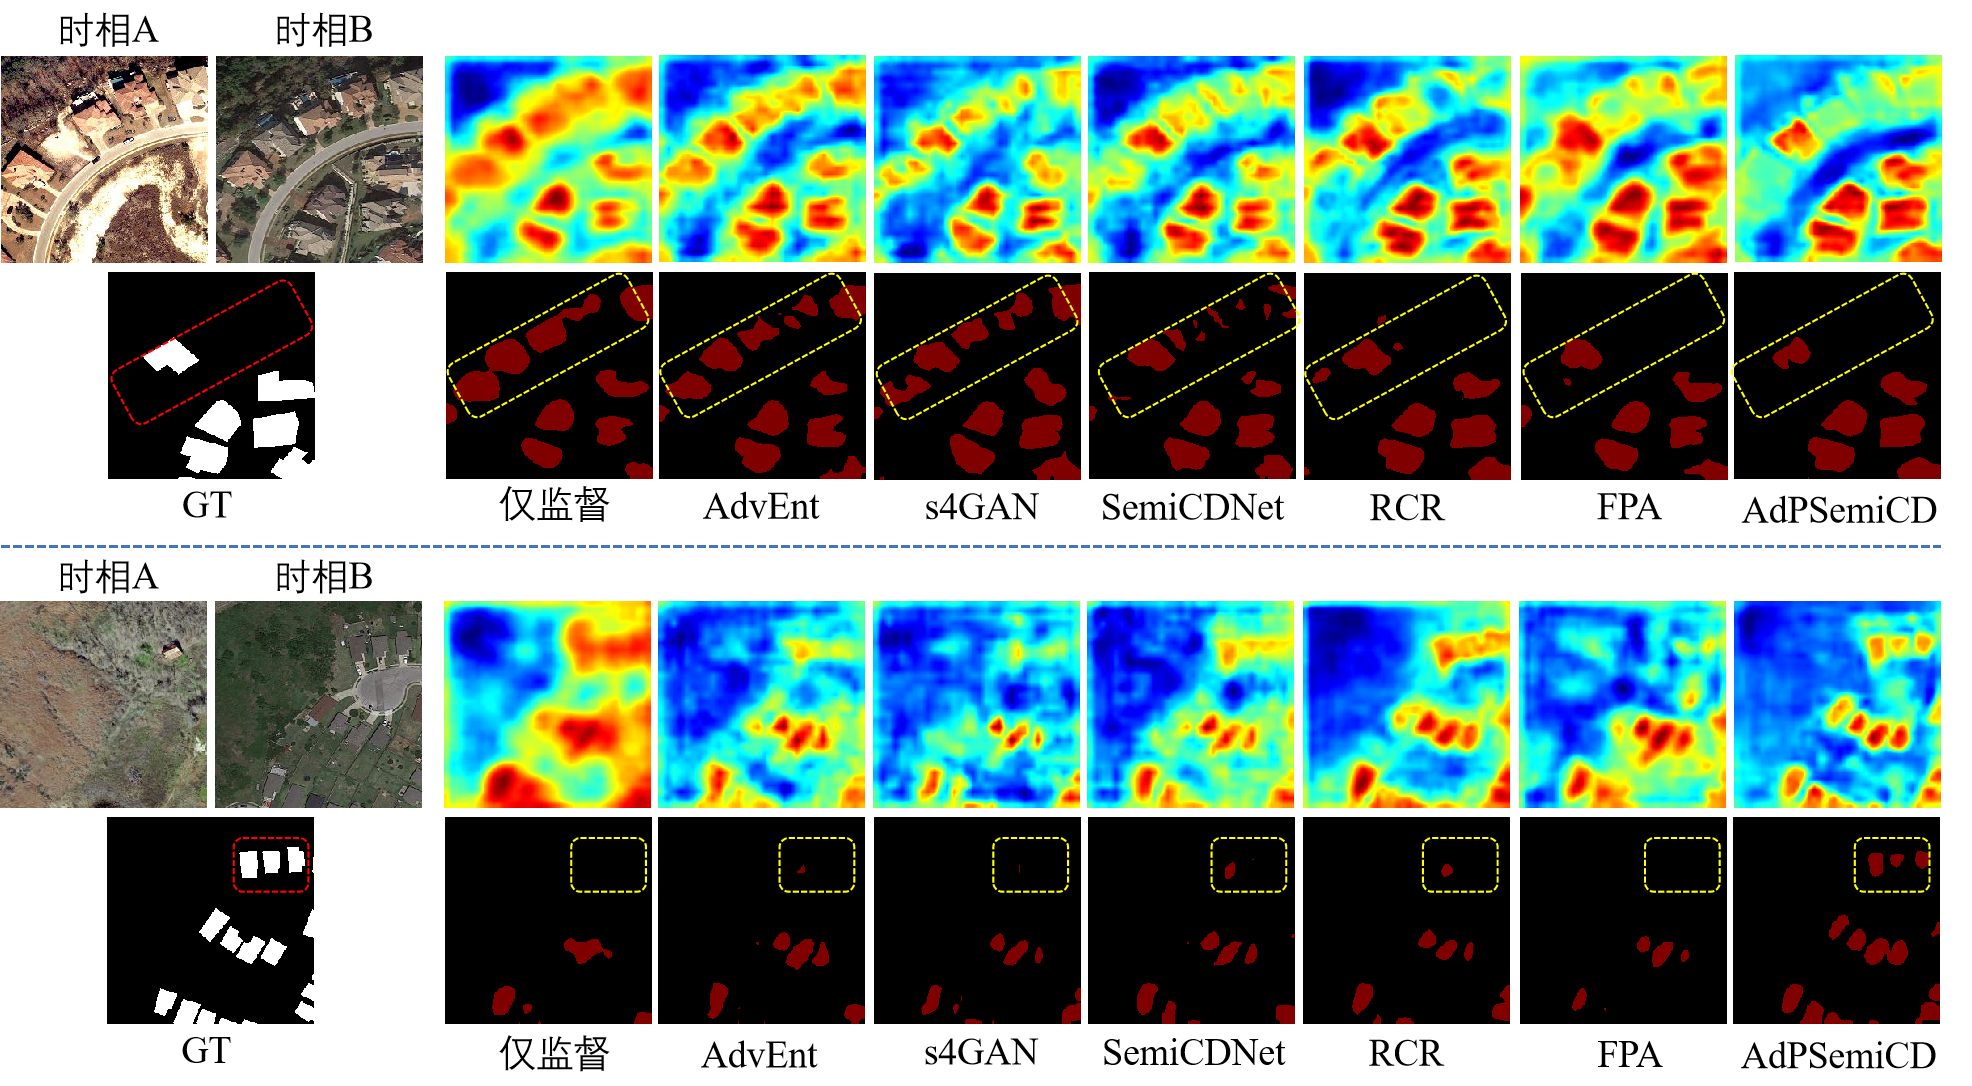
\includegraphics[scale=0.45]{images/AdPlevir-vis.png}
  \caption{
    5$\%$标记训练样本下AdPSemiCD与SOTA方法在LEVIR-CD测试集上的可视化对比图
  }
  \label{fig:AdPLevir-vis}
\end{figure}
\begin{figure}[!htbp]
  \centering
  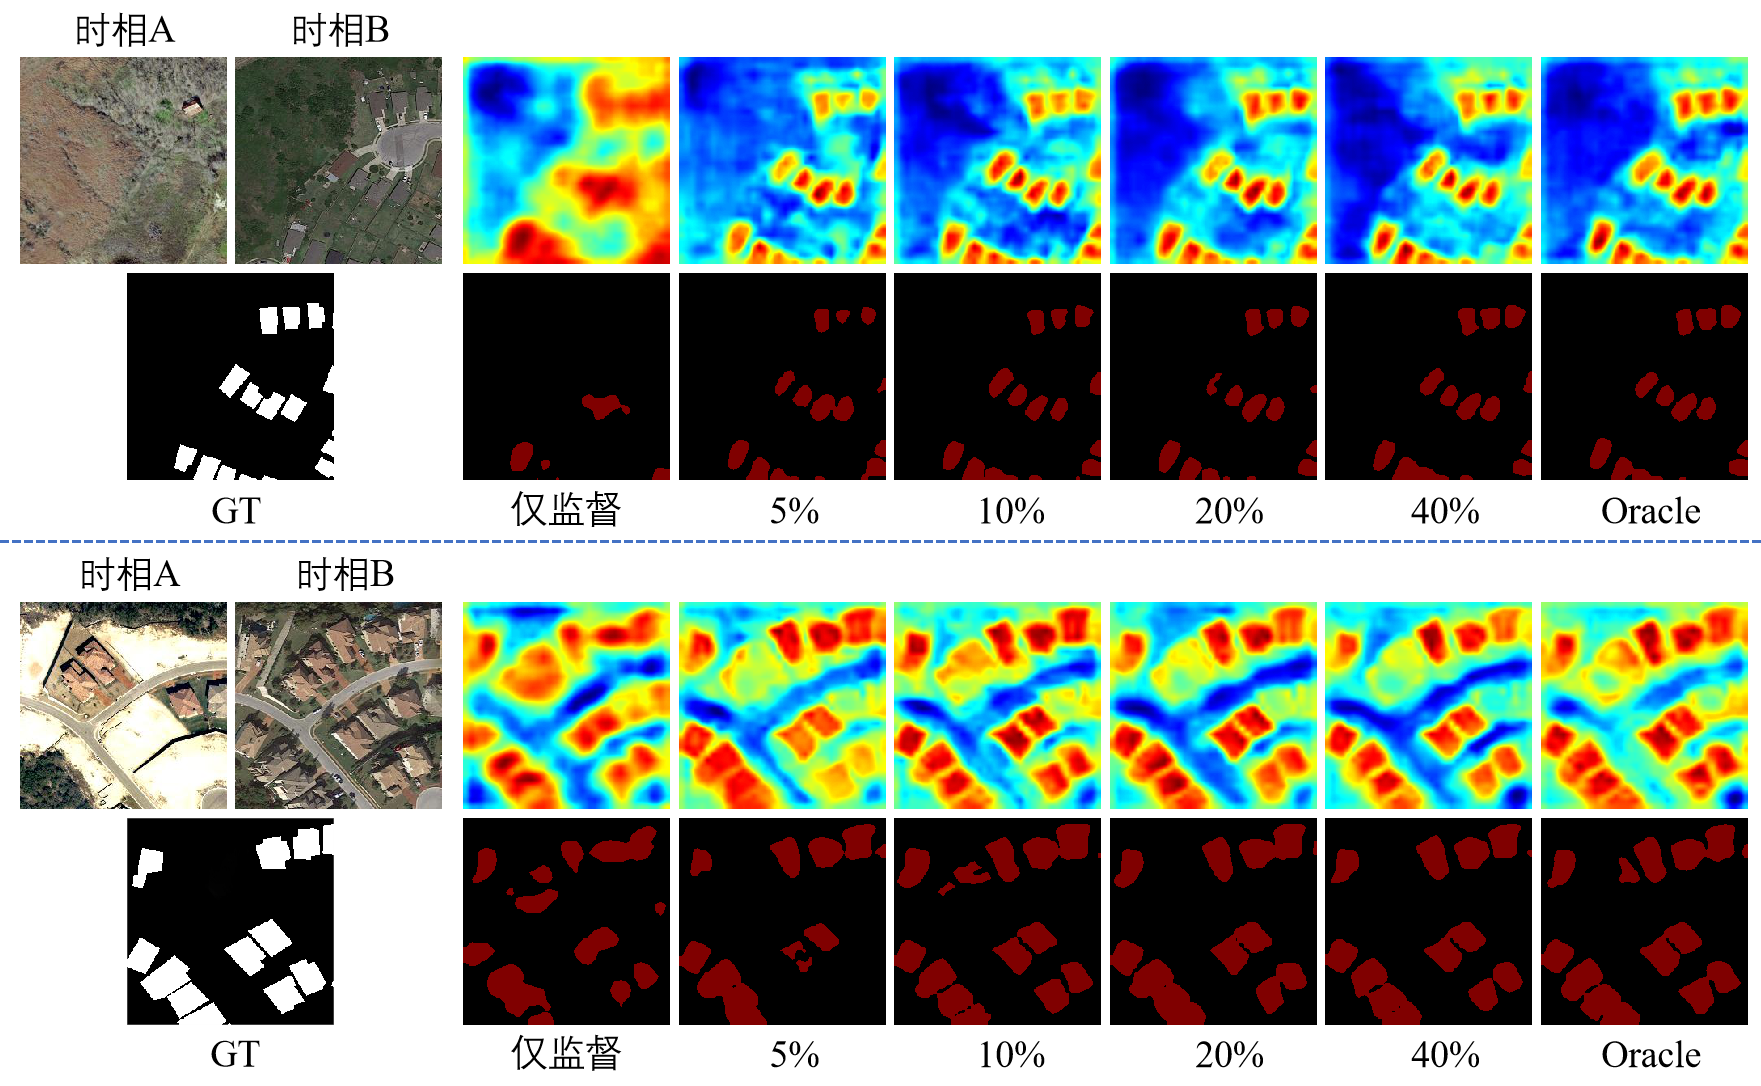
\includegraphics[scale=0.45]{images/AdPdiffSemi.png}
  \caption{
    不同标记率下AdPSemiCD在LEVIR-CD测试集上的可视化对比图
  }
  \label{fig:AdPdiffLEVIR-vis}
\end{figure}
我们还对所有对比实验中的检测结果进行了可视化,图\ref{fig:AdPLevir-vis}、\ref{fig:AdPWhu-vis}、\ref{fig:AdPCdd-vis}、\ref{fig:AdPCl-vis}分别展示了在LEVIR-CD、WHU-CD、CDD、CL-CD四个数据集的测试集上的一些变化检测结果样例,同时以热力图和二值标签的形式对模型预测结果进行了可视化表示。整体看来,本章提出的AdPSemiCD相比其余半监督变化检测方法在检测效果上都表现更佳,尤其是与使用随机特征扰动的RCR方法相比。此外,从热力图分布可以看出,在仅监督训练模式下,模型的预测概率比较分散,进一步可以推断出预测信息熵较高。半监督方法一定程度上可以更加自信地判别出变化和不变区域,表现在热力图上两类区别更加明显,高热区域更加集中,表明了半监督学习利用大量无标记样本的有效性,但是仍然存在一些判别错误的情况,我们的AdPSemiCD有效减轻了这一现象,取得了更好的表现。
\begin{figure}[!htbp]
  \centering
  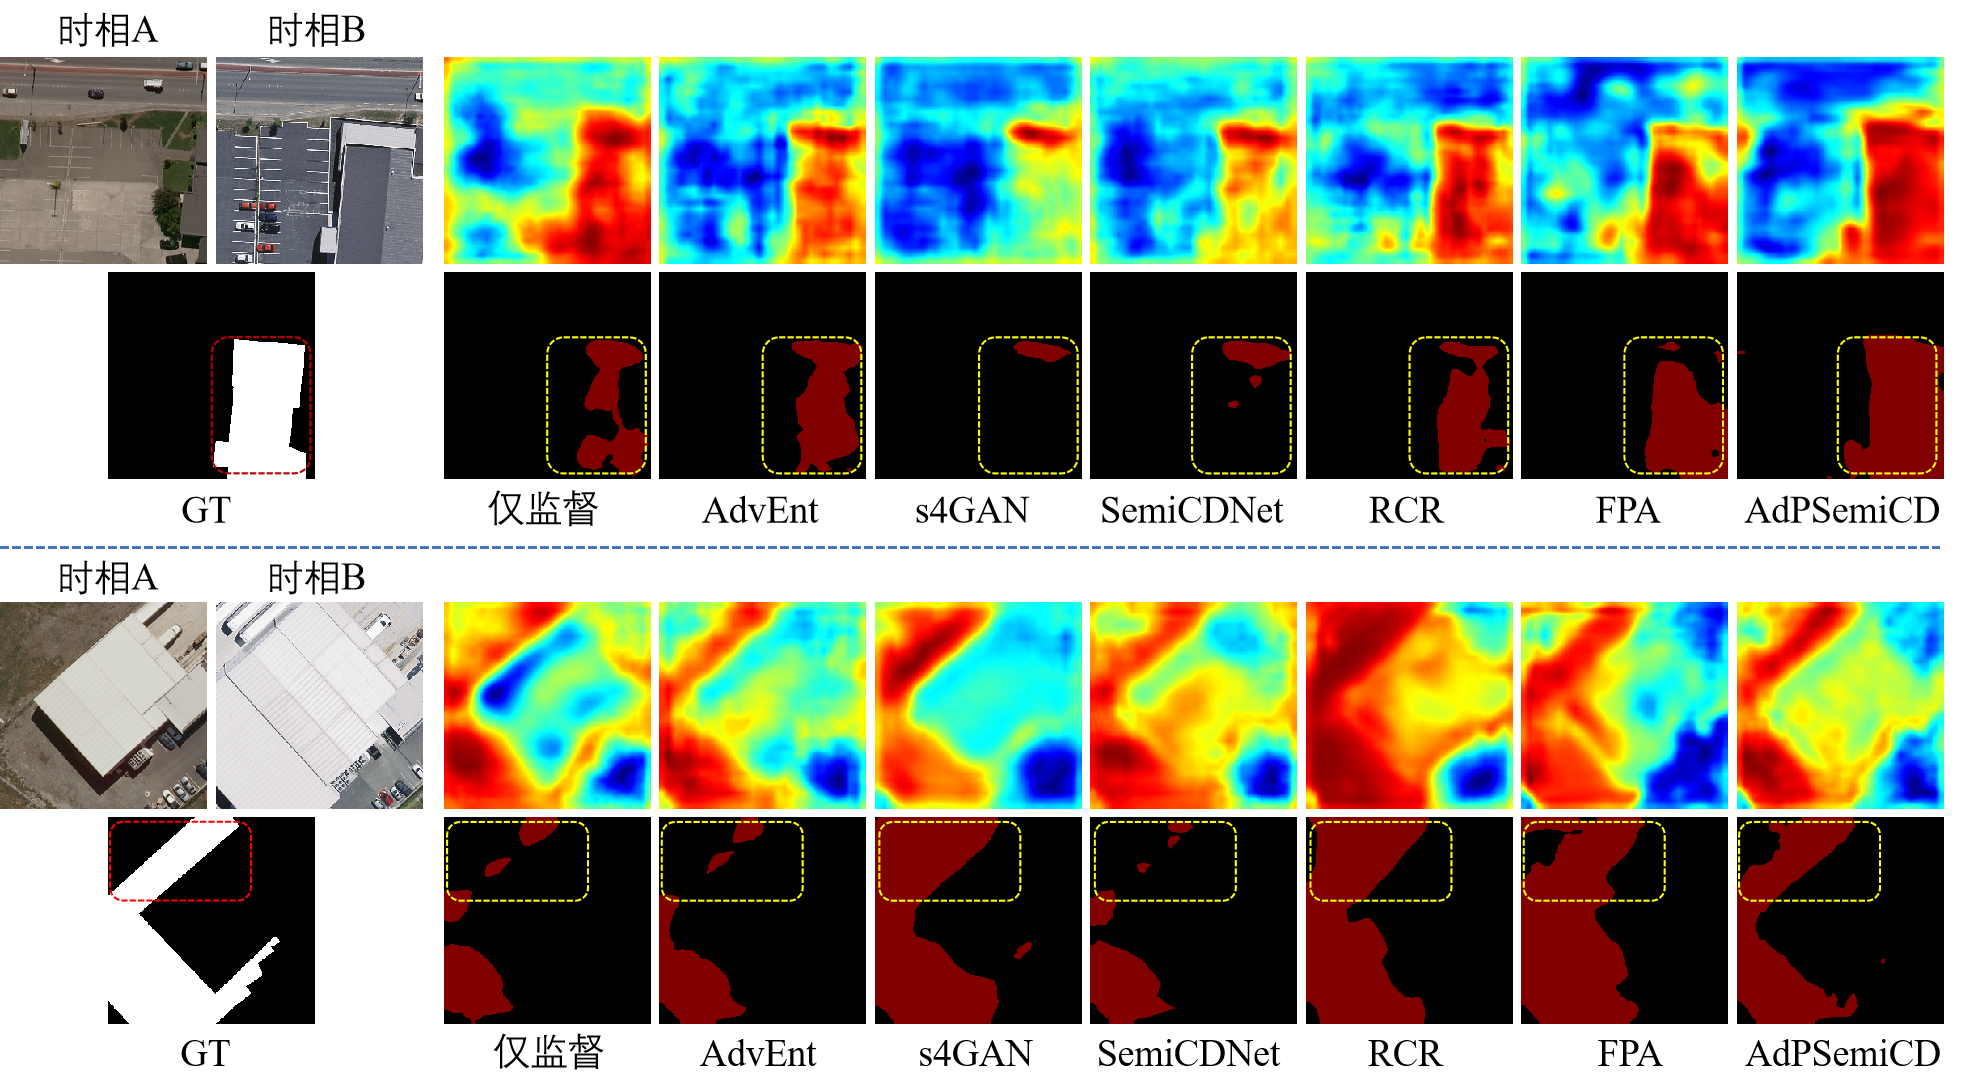
\includegraphics[scale=0.45]{images/AdPwhu-vis.png}
  \caption{
    5$\%$标记训练样本下AdPSemiCD与SOTA方法在WHU-CD测试集上的可视化对比图
  }
  \label{fig:AdPWhu-vis}
\end{figure}

具体地说,LEVIR-CD数据集上的可视化结果展示了本章方法在减少漏检以及小目标变化检测上的优异表现,相比其他方法,RCR已经取得了一定的进步,而在其扰动方式上的针对性改进使得我们的方法进一步提高了性能。在WHU-CD数据集上,所选样例与背景的相似度极高,在第一组结果中大部分方法漏检严重,仅识别出了与背景差异较大的小部分变化区域,而第二组的结果中则是错误地将左上角的其他类别检测为建筑物变化区域。从热力图和标签图上都可以看出,本章方法能够以更高的置信度检测出来边界更加清晰的变化区域。在多类别的数据集上,本章方法同样表现很好,例如在CDD数据集的可视化结果中,AdPSemiCD不仅在小目标(车辆)的变化检测上继承了RCR不俗的性能,在容易混淆的变化目标上同样准确地进行了检测识别。值得一提的是,从可视化结果上看,本章方法很好地弥补了第三章由于样本改造产生类别学习样本缺失进而造成的细长目标识别失效的问题,如图\ref{fig:AdPCdd-vis}中第二组结果所示,最为直观地证明了本章方法达成了研究目的。对于Cl-CD数据集,由于样本量太少,导致所有方法整体上检测效果都比较差,但正是在这样一种极端情况下,在图\ref{fig:AdPCl-vis}所示的两组样例中,我们的方法在这类小目标变化上仍然表现出了强大的检测能力。
\begin{figure}[!htbp]
  \centering
  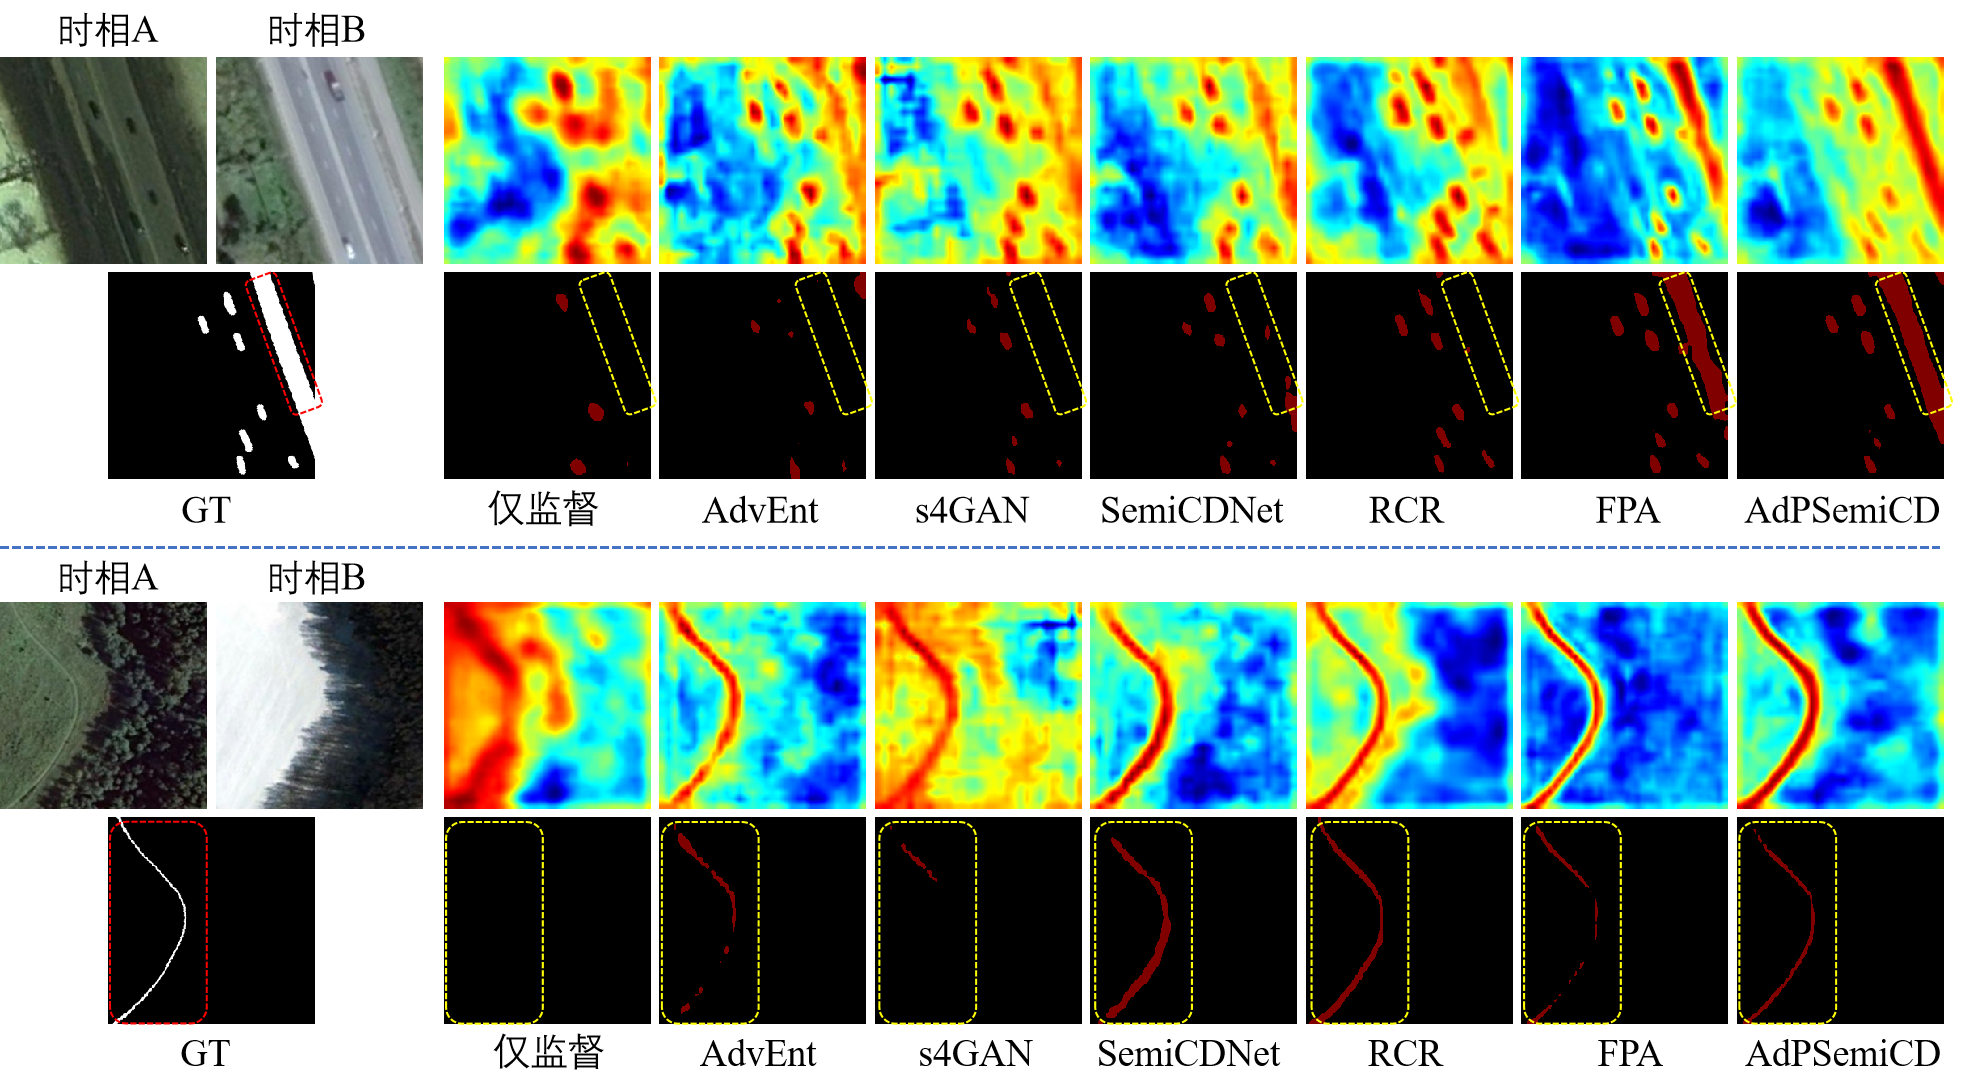
\includegraphics[scale=0.45]{images/AdPcdd-vis.png}
  \caption{
    5$\%$标记训练样本下AdPSemiCD与SOTA方法在CDD测试集上的可视化对比图
  }
  \label{fig:AdPCdd-vis}
\end{figure}

我们还对LEVIR-CD数据集上,在不同半监督设置下的检测结果进行了可视化,如图\ref{fig:AdPdiffLEVIR-vis}所示。首先最为显而易见的就是,我们的半监督变化检测方法所取得的检测效果相比仅监督基线提升了很多,无论是在整体识别准确率还是边界处理上都要好。随着提供的标记数据越多,变化检测性能也更好,这也从侧面反映了变化检测任务对人工标注的依赖,可以看到Oracle(即使用整个标注训练集进行训练)和5$\%$仅监督的基线之间存在非常明显的差距,因此就凸显了半监督变化检测的意义。我们的AdPSemiCD在5$\%$标记数据上的训练效果就已经基本能够胜任变化检测任务,在10$\%$至10$\%$标记数据下就已经取得了和Oracle相当的性能,这也证明了我们的方法具有很大的应用价值。

总的来说,这些可视样例代表性地展示了本章方法与其他方法的变化检测效果对比,与定性结果相对应,AdPSemiCD在所有数据集上的检测效果从可视化结果来看,都比RCR更好,这得益于其不仅保留了RCR中探索出的广阔的特征扰动空间对半监督变化检测更加有利这一成功经验,同时还借鉴了前文中对不同无标记样本进行自适应训练的设计,为无标记样本创造了一个自适应的可控特征扰动空间,不仅提高了模型的泛化性,还减少了确认偏差带来的负面影响,从而稳定地提升了半监督变化检测性能。
\begin{figure}[!htbp]
  \centering
  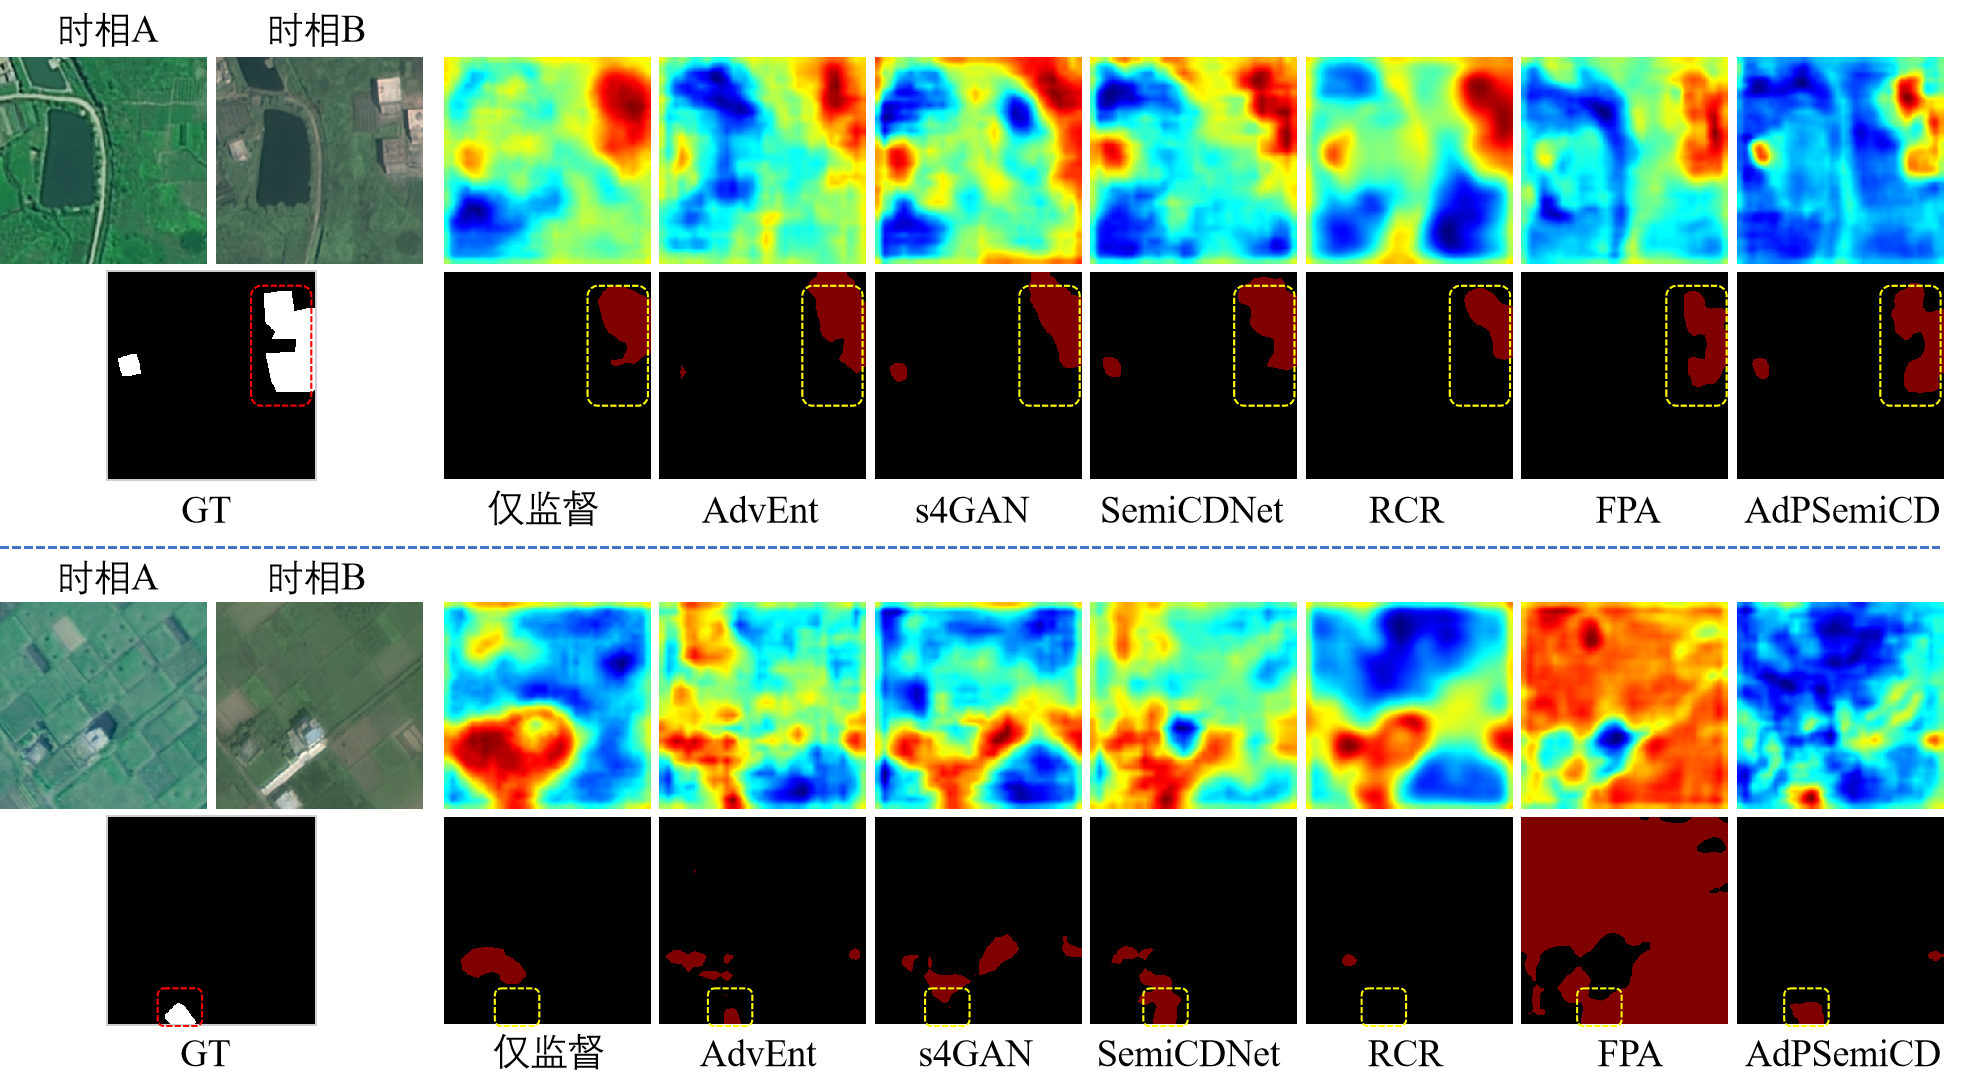
\includegraphics[scale=0.45]{images/AdPcl-vis.png}
  \caption{
    5$\%$标记训练样本下AdPSemiCD与SOTA方法在CL-CD测试集上的可视化对比图
  }
  \label{fig:AdPCl-vis}
\end{figure}
\subsection{消融实验}
\begin{table*}[tb]
  % \renewcommand\arraystretch{1.2}
\centering
% \tiny
\caption{AdPSemiCD在WHU-CD数据集上的消融实验}
   \resizebox{0.9\textwidth}{!}{
   % \setlength{\tabcolsep}{9pt}
\begin{tabular}{p{30mm}p{20mm}p{20mm}cp{20mm}p{20mm}cp{20mm}p{20mm}cp{20mm}p{20mm}} %
  \toprule
  \multirow{2}{*}{\parbox[c]{.2\linewidth}{Method}} & \multicolumn{2}{c}{5\%} & & \multicolumn{2}{c}{10\%} & & \multicolumn{2}{c}{20\%} & & \multicolumn{2}{c}{40\%}\\
  \cmidrule{2-3} \cmidrule{5-6} \cmidrule{8-9} \cmidrule{11-12}
  & {$IoU^c$} & {OA} && {$IoU^c$} & {OA} & & {$IoU^c$} & {OA} &&{$IoU^c$} & {OA}\\
  \midrule
  仅监督   &   50.0 & 97.48 && %5
                  55.7 & 97.53 && %10
                  65.4 & 98.20 && %20
                  76.1 & 98.94 \\ %40
  MT+NP      &   61.0 {\color{red} (+11.0)} & 98.08 {\color{red}(+0.60)} &&
                  62.4 {\color{red} (+6.7)} & 98.16 {\color{red} (+0.63)} &&
                  70.7 {\color{red} (+5.3)} & 98.69 {\color{red} (+0.49)}&&
                  77.5 {\color{red} (+1.4)} & 98.99 {\color{red} (+0.05)} \\
  MT+FP     &   61.4 {\color{red} (+11.4)}& 98.15 {\color{red} (+0.67)} &&
                  63.7 {\color{red} (+8.0)} & 98.28 {\color{red} (+0.75)} &&
                  73.2 {\color{red} (+7.8)} & 98.80 {\color{red} (+0.60)} &&
                  77.1 {\color{red} (+1.0)} & 98.96 {\color{red} (+0.02)} \\
  MT+RP &  66.1 {\color{red} (+16.1)} & 98.40 {\color{red} (+0.92)} && %5
                68.7   {\color{red} (+13.0)} & 98.53 {\color{red} (+1.00)} && %10
                75.6 {\color{red} (+10.2)} & 98.88 {\color{red} (+0.68)} && %20
                  78.0 {\color{red} (+1.9)} & 98.98 {\color{red} (+0.04)} \\ %40
  AdPSemiCD   &   66.9 {\color{red} (+16.7)} & 98.54 {\color{red} (+1.06)} &&
                  69.3 {\color{red} (+13.6)} & 98.65 {\color{red} (+1.12)} &&
                  77.2 {\color{red} (+11.8)} & 98.94 {\color{red} (+0.74)} &&
                  78.9 {\color{red} (+2.8)} & 99.09 {\color{red} (+0.15)} \\
  \bottomrule
\end{tabular}
  }
% \normalsize
\label{tab:ablation_AdPModel}
\end{table*}
为了证明本章提出的自适应特征扰动有效,我们同样从定量和定性两个角度设计了消融实验。首先是在平均教师半监督学习框架之上,分别使用无特征扰动、RCR中的随机特征扰动以及本章提出的自适应特征扰动,将前两组实验作为对照组。首先对图表中使用的缩写做出说明:

NP:无特征扰动,即直接将教师模型、学生模型预测概率分布的均方误差作为训练损失;

FP:Fixed Perturbation,固定特征扰动,即根据经验预定义扰动强度和扰动数量;

RP:Random Perturbation,随机特征扰动,即RCR中使用的随机选择扰动强度和扰动数量;

最终在WHU-CD上取得的实验指标结果如表\ref{tab:ablation_AdPModel}所示,其中红色标注部分为该方法相比基线的提升值。在不进行特征扰动时,模型退化为平均教师模型实现的FixMatch方法,可以在基线之上大幅度地提高模型性能。使用固定特征扰动并不能进一步带来更大的改进,一方面是因为单一的固定扰动参数值很难确定最优选择,另一方面,对困难样本进一步继续施加扰动,会扩大确认偏差,所以尤其是在标记训练数据更少时,固定特征扰动带来的收益更加微乎其微。RCR中使用的随机特征扰动具有一定的前景,相比固定扰动方案,它纳入了更多的随机性,对不同样本施加不同程度的扰动,很大程度上提高了模型的泛化性能。最后本章提出的自适应特征扰动方案进一步细化了扰动的过程,对样本进行评估,进而基于此评估自适应地调整扰动参数和数量,因此继续提升了模型的性能并且提高了稳定性。

此外,我们还对无监督损失的权重进行了消融实验,本章采取的权重与第三章相同,由公式\ref{eq:ramp-up}计算,其计算主要由$\gamma$和$w_{max}$两个参数决定。因此我们对这两个参数的选择组合进行了消融研究,如表\ref{tab:AdPPram_ablation}所示,展示了我们在LEVIR-CD、WHU-CD、CDD、CL-CD四个数据集上10$\%$标记率下取得的实验结果。我们先固定最大权重值$w_{max}$为1.0,将$\gamma$作为变量控制预热进程的快慢,得到每个数据集上$\gamma$的最佳参数,在LEVIR-CD、WHU-CD、CDD和CL-CD上其最佳取值分别为:0.1,0.1,0.5,0.1。在确定$\gamma$取值的基础之上,再将$w_{max}$作为唯一变量,探索预热完成后最大无监督权重的整个模型的影响,确定其最佳参数选择,实验结果表明在LEVIR-CD、WHU-CD、CDD和CL-CD上其最佳取值分别为:30.0,30.0,30.0,10.0。由此,可以得出基本结论,即训练数据量越小,$\gamma$取值应该越小,否则过拟合的可能性越高;多类别数据集上$\gamma$取值应该比单一类别(建筑物)变化检测数据集上更大,模型应该充分学习标记样本中各个类别的语义特征;$w_{max}$取值应该比较大,因为同一样本不同扰动版本之间的均方误差值数量级较小,给予一个较大的权重才能够使其对模型训练发挥作用。因此,在其余数据集上我们基于此经验,选择的取值组合为分别为:LEVIR-CD+(0.1,30.0);GZ-CD:(0.05,10.0);EGY-CD:(0.1,10.0);HRCUS-CD:(0.1,30.0);DSIFN-CD:(0.5,30.0);SYSU-CD:(0.5,30.0),对比实验中的所有实验结果即在此参数组合下所取得,实验证明我们的取值经验是有效的,不过在逐个数据集上都进行更细致的调参过程或许会取得更好的实验结果。
\begin{table*}[!htbp]
  % \renewcommand\arraystretch{1.2}
\centering
% \tiny
\caption{超参数敏感性消融实验结果}
   \resizebox{0.9\textwidth}{!}{
   % \setlength{\tabcolsep}{9pt}
   \begin{tabular}{p{10mm}p{20mm}p{5mm}cp{10mm}p{5mm}cp{10mm}p{5mm}cp{10mm}p{5mm}cp{10mm}p{5mm}} %
  \toprule
  \multirow{2}{*}{\parbox[c]{.1\linewidth}{$\gamma$}} & \multirow{2}{*}{$w_{max}$} & \multicolumn{2}{c}{LEVIR-CD} & & \multicolumn{2}{c}{WHU-CD} & & \multicolumn{2}{c}{CDD} & & \multicolumn{2}{c}{CL-CD}\\
  \cmidrule{3-4} \cmidrule{6-7} \cmidrule{9-10} \cmidrule{12-13}
  && {$IoU^c$} & {OA} && {$IoU^c$} & {OA} & & {$IoU^c$} & {OA} && {$IoU^c$} & {OA}\\
  \midrule
  0  & 0 (Sup.Only) &   66.8 & 98.13 && %LEVIR-CD
                  55.7 & 97.53 && %WHU-CD
                  67.9 & 95.46 &&  %CDD
                  31.4 & 92.42 \\  %CL-CD
  0.1   & 1.0   & 69.5 & 98.37 && %LEVIR-CD
                  60.1 & 97.96 && %WHU-CD
                  69.9 & 95.85 &&  %CDD
                  33.7 & 93.15 \\  %CL-CD
  0.5   & 1.0   & 68.0 & 98.24 && %LEVIR-CD
                  59.9 & 97.92 && %WHU-CD
                  71.4 & 96.05 &&  %CDD
                  31.8 & 92.68 \\  %CL-CD
  1.0   & 1.0   & 67.0 & 98.16 && %LEVIR-CD
                  57.8 & 97.84 && %10
                  70.2 & 95.93 &&  %CDD
                  30.6 & 92.28 \\  %CL-CD
  0.1   & 0.5   & 66.5 & 98.13 && %LEVIR-CD
                  58.4 & 97.90 && %WHU-CD
                  - & - &&  %CDD
                  31.7 & 92.75 \\  %CL-CD
  0.1   & 5.0   & 74.4 & 98.52 && %LEVIR-CD
                  65.6 & 98.23 && %WHU-CD
                  - & - &&  %CDD
                  34.9 & 93.29 \\  %CL-CD
  0.1   & 10.0  & 75.6 & 98.65 && %LEVIR-CD
                  68.1 & 98.47 && %WHU-CD
                  - & - &&  %CDD
                  \underline{\textbf{36.1}} &
                  \underline{\textbf{93.55}} \\  %CL-CD
  0.1   & 30.0  & \underline{\textbf{76.9}} &
                  \underline{\textbf{98.70}} && %LEVIR-CD
                  \underline{\textbf{69.3}} &
                  \underline{\textbf{98.65}} && %WHU-CD
                  - & - &&  %CDD
                  33.5 & 93.07 \\  %CL-CD
  0.5   & 0.5   & - & - && %LEVIR-CD
                  - & - && %WHU-CD
                  70.1 & 95.79 &&  %CDD
                  - & - \\  %CL-CD
  0.5   & 5.0   & - & - && %LEVIR-CD
                  - & - && %WHU-CD
                  74.8 & 96.57 &&  %CDD
                  - & - \\  %CL-CD
  0.5   & 10.0  & - & - && %LEVIR-CD
                  - & - && %WHU-CD
                  \underline{\textbf{77.5}} &
                  \underline{\textbf{96.90}} &&  %CDD
                  - & - \\  %CL-CD
  0.5   & 30.0  & - & - && %LEVIR-CD
                  - & - && %WHU-CD
                  66.2 & 96.73 &&  %CDD
                  - & - \\  %CL-CD
  \bottomrule
\end{tabular}
  }
% \normalsize
\label{tab:AdPPram_ablation}
\end{table*}
\begin{figure}[H]
  \centering
  \hspace*{\fill} % 左侧留空
  \begin{subfigure}[t]{0.46\textwidth} % 左图占45%宽度
      \centering
      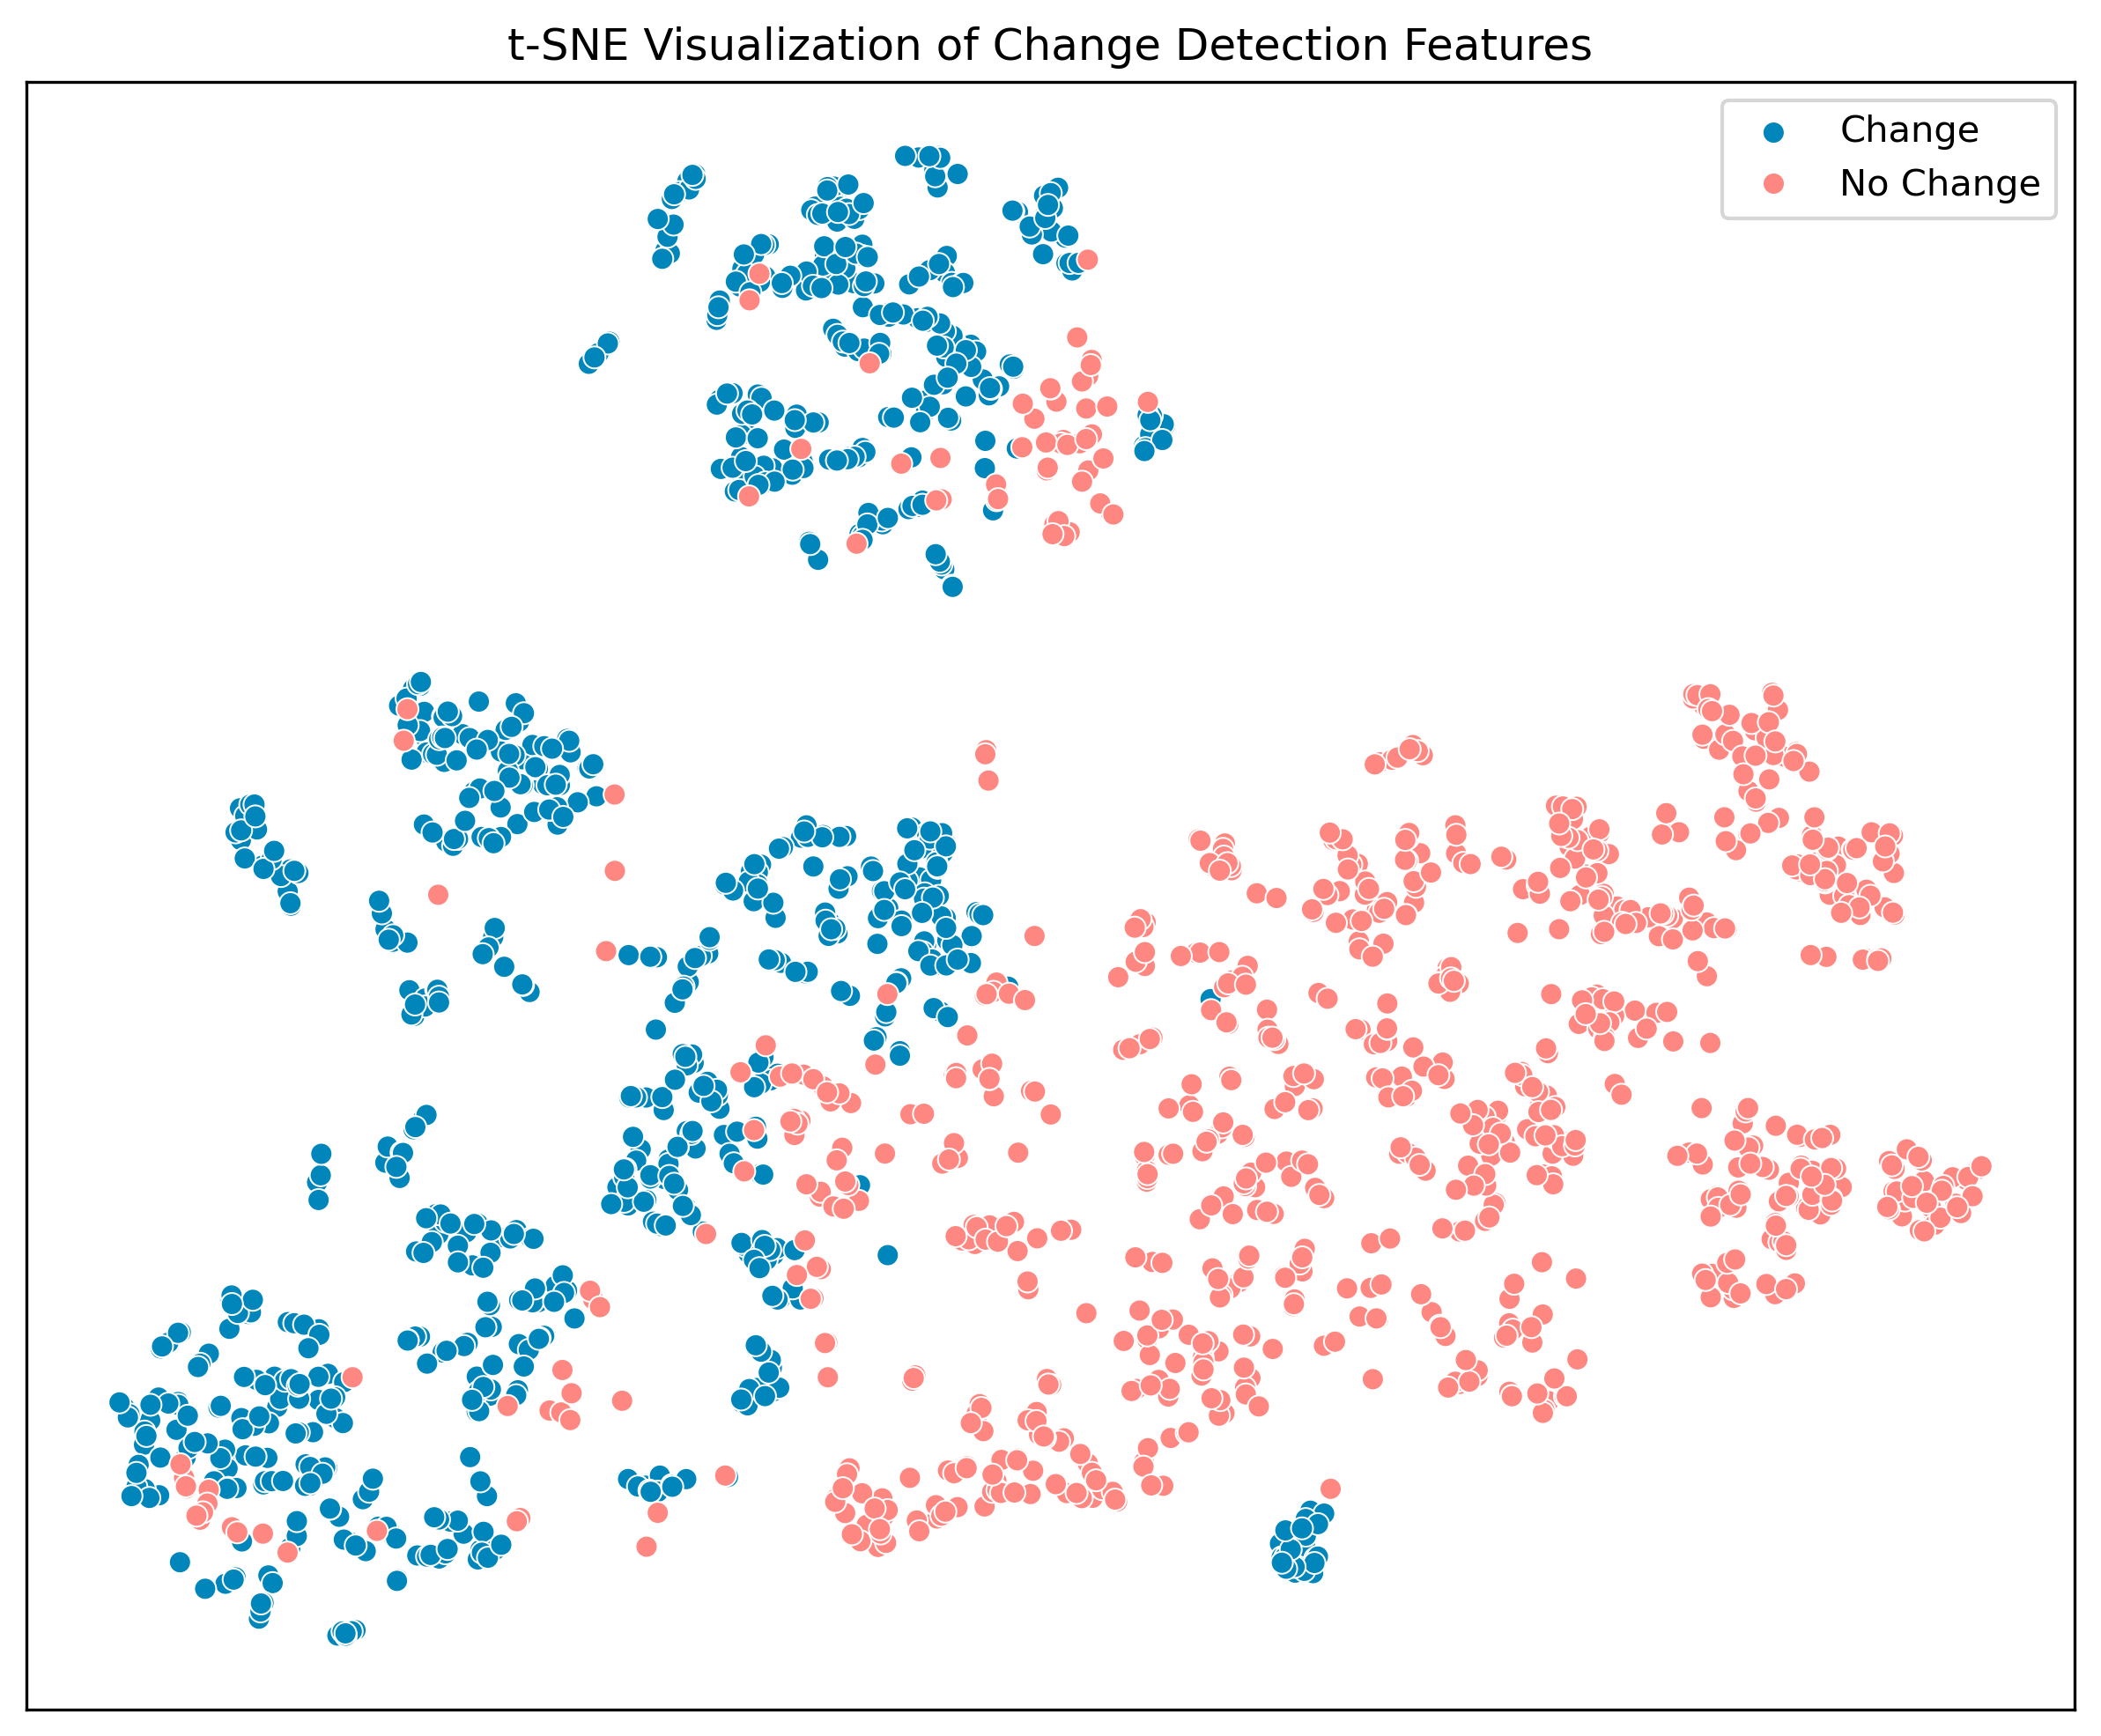
\includegraphics[scale=0.36]{images/tsne_5RCRl.png}
      \caption{RCR随机扰动}
      \label{fig:tsneL_left}
  \end{subfigure}
  \hfill % 两图之间留空
  \begin{subfigure}[t]{0.46\textwidth} % 右图占45%宽度
      \centering
      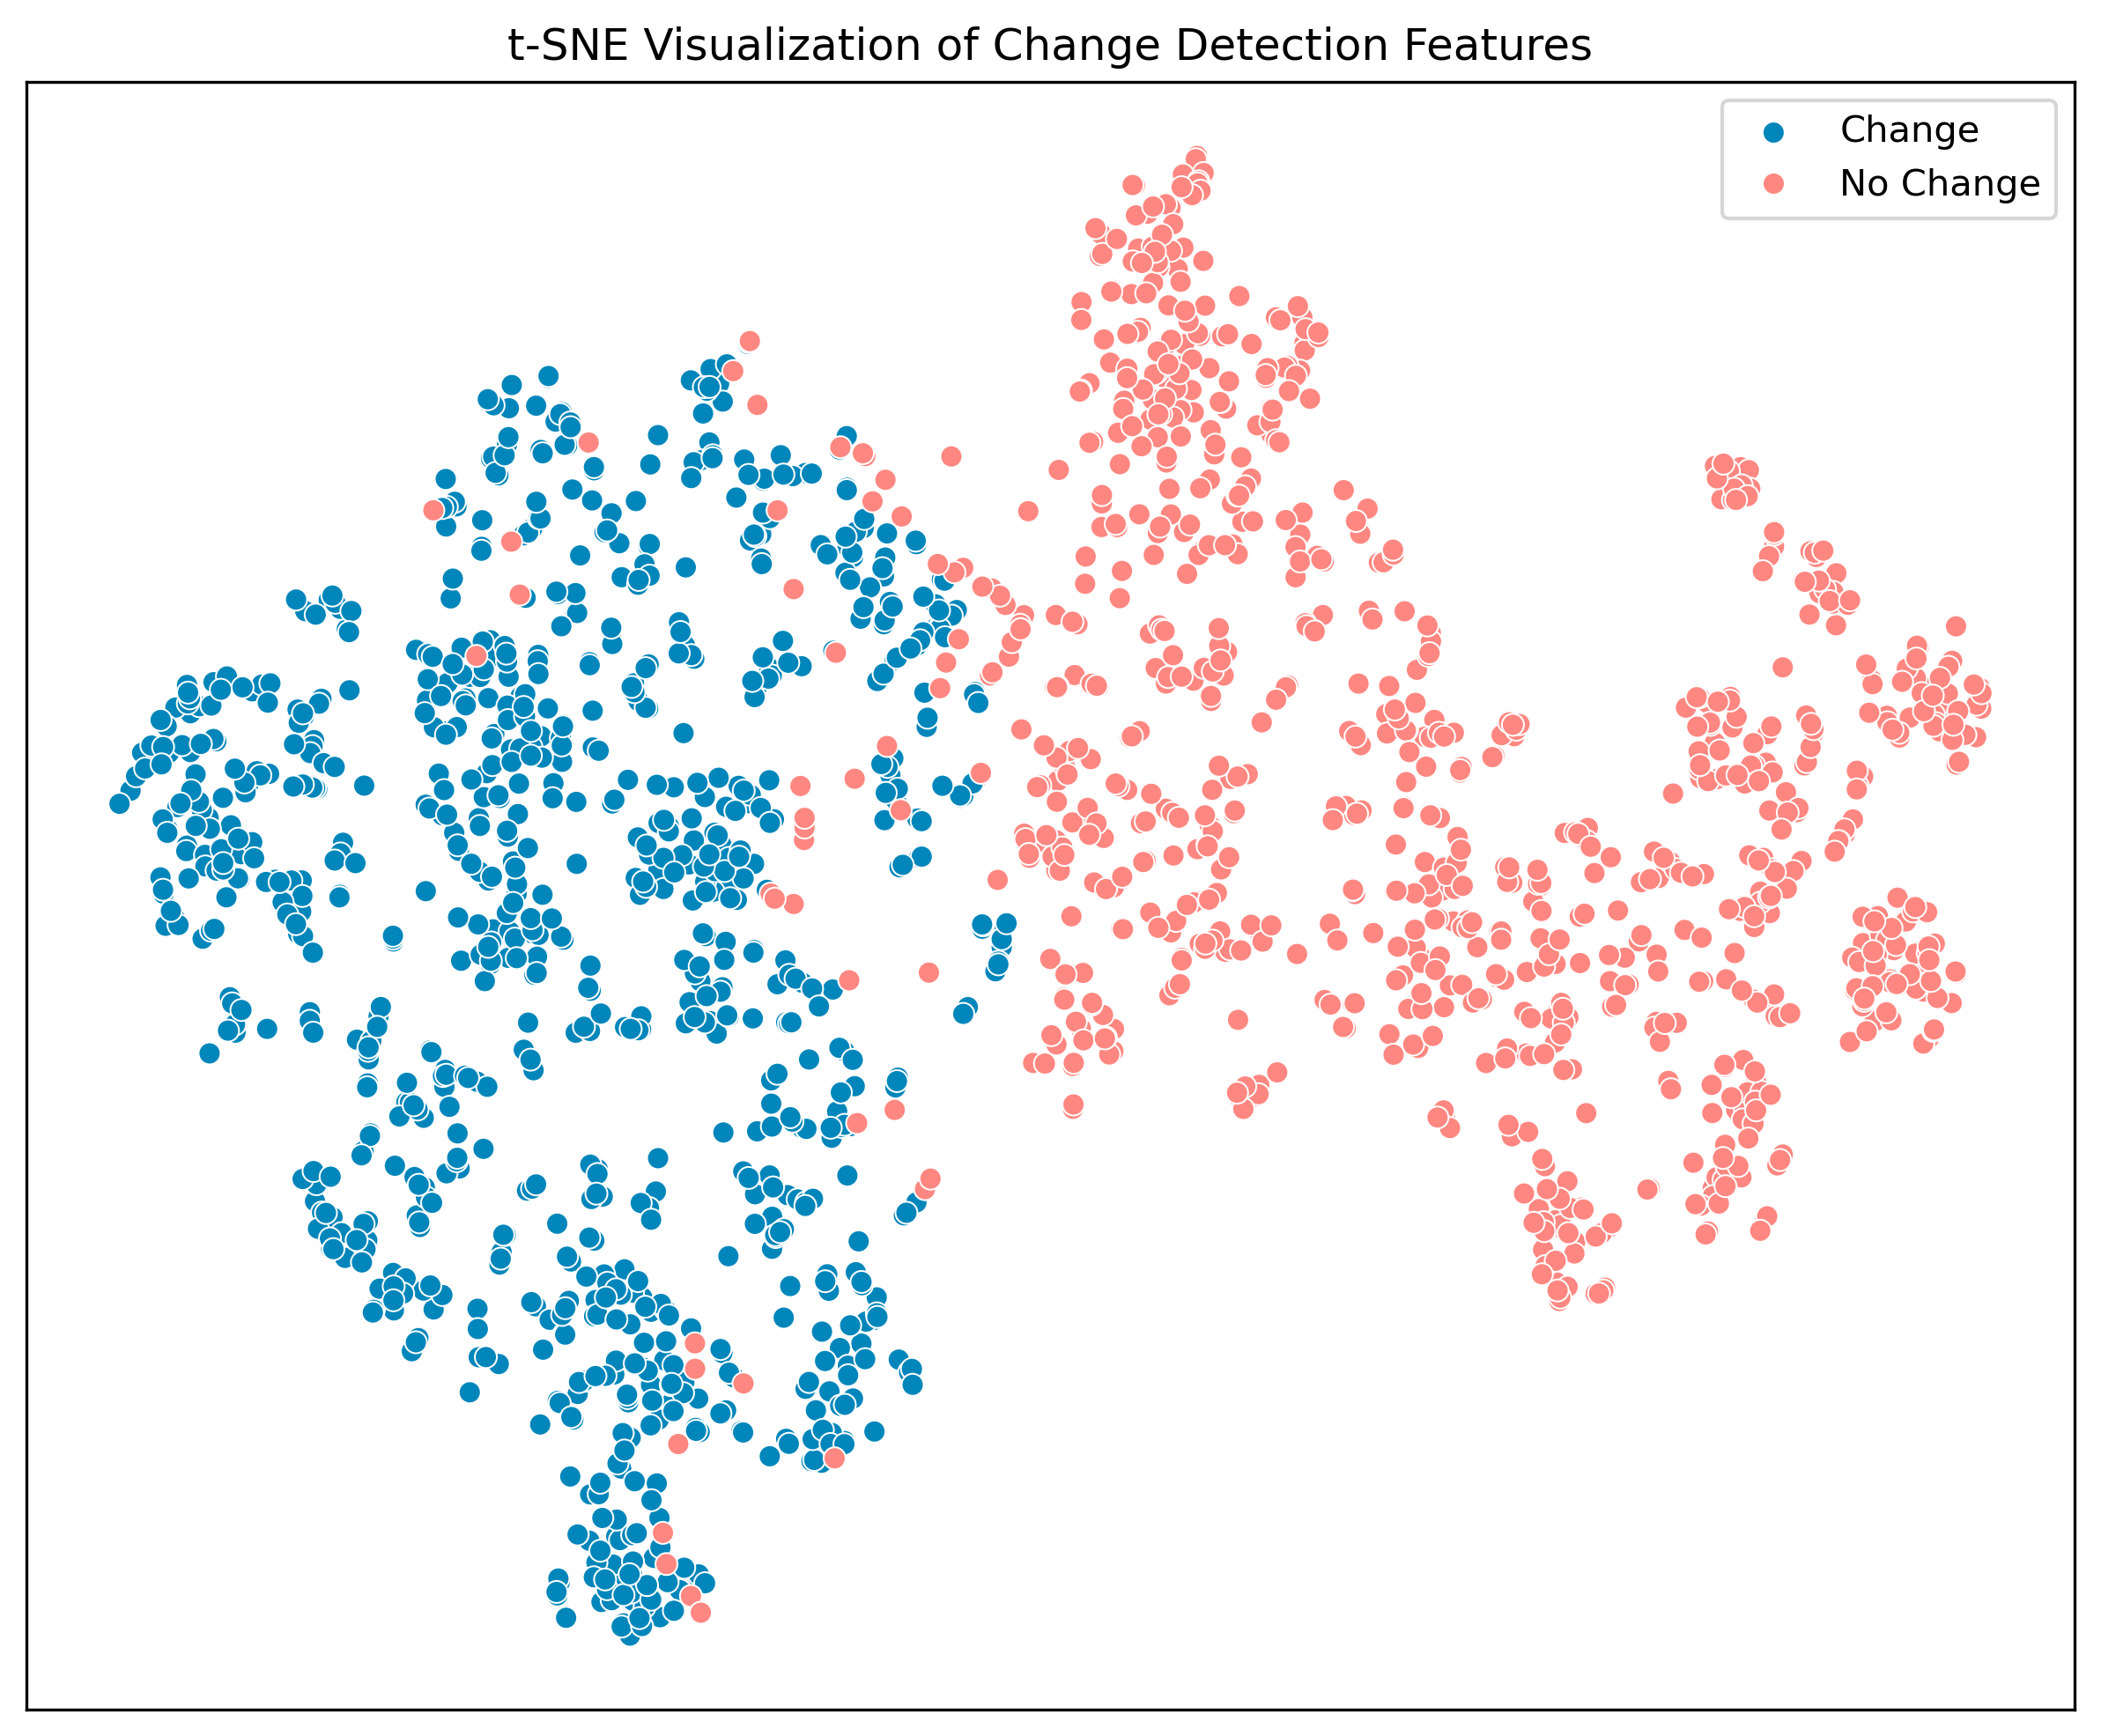
\includegraphics[scale=0.36]{images/tsne_5AdPl.png} % 替换为右图路径
      \caption{AdPSemiCD自适应扰动} % 修改为右图的标题
      \label{fig:tsneL_right}
  \end{subfigure}
  \hspace*{\fill} % 左侧留空
  \caption{LEVIR-CD测试集上的t-SNE特征可视化对比}
  \label{fig:AdP_tsneL}
\end{figure}

最后,我们还使用t-SNE技术对分别使用随机特征扰动和自适应特征扰动时测试集上的特征进行了降维并投影到二维坐标进行了可视化,可视化结果如图\ref{fig:AdP_tsneL}、图\ref{fig:AdP_tsneW}、图\ref{fig:AdP_tsneC}以及图\ref{fig:AdP_tsneCL}分别为LEVIR-CD、WHU-CD、CDD和CL-CD数据集上的t-SNE特征可视化结果。
\begin{figure}[H]
  \centering
  \hspace*{\fill} % 左侧留空
  \begin{subfigure}[t]{0.46\textwidth} % 左图占45%宽度
      \centering
      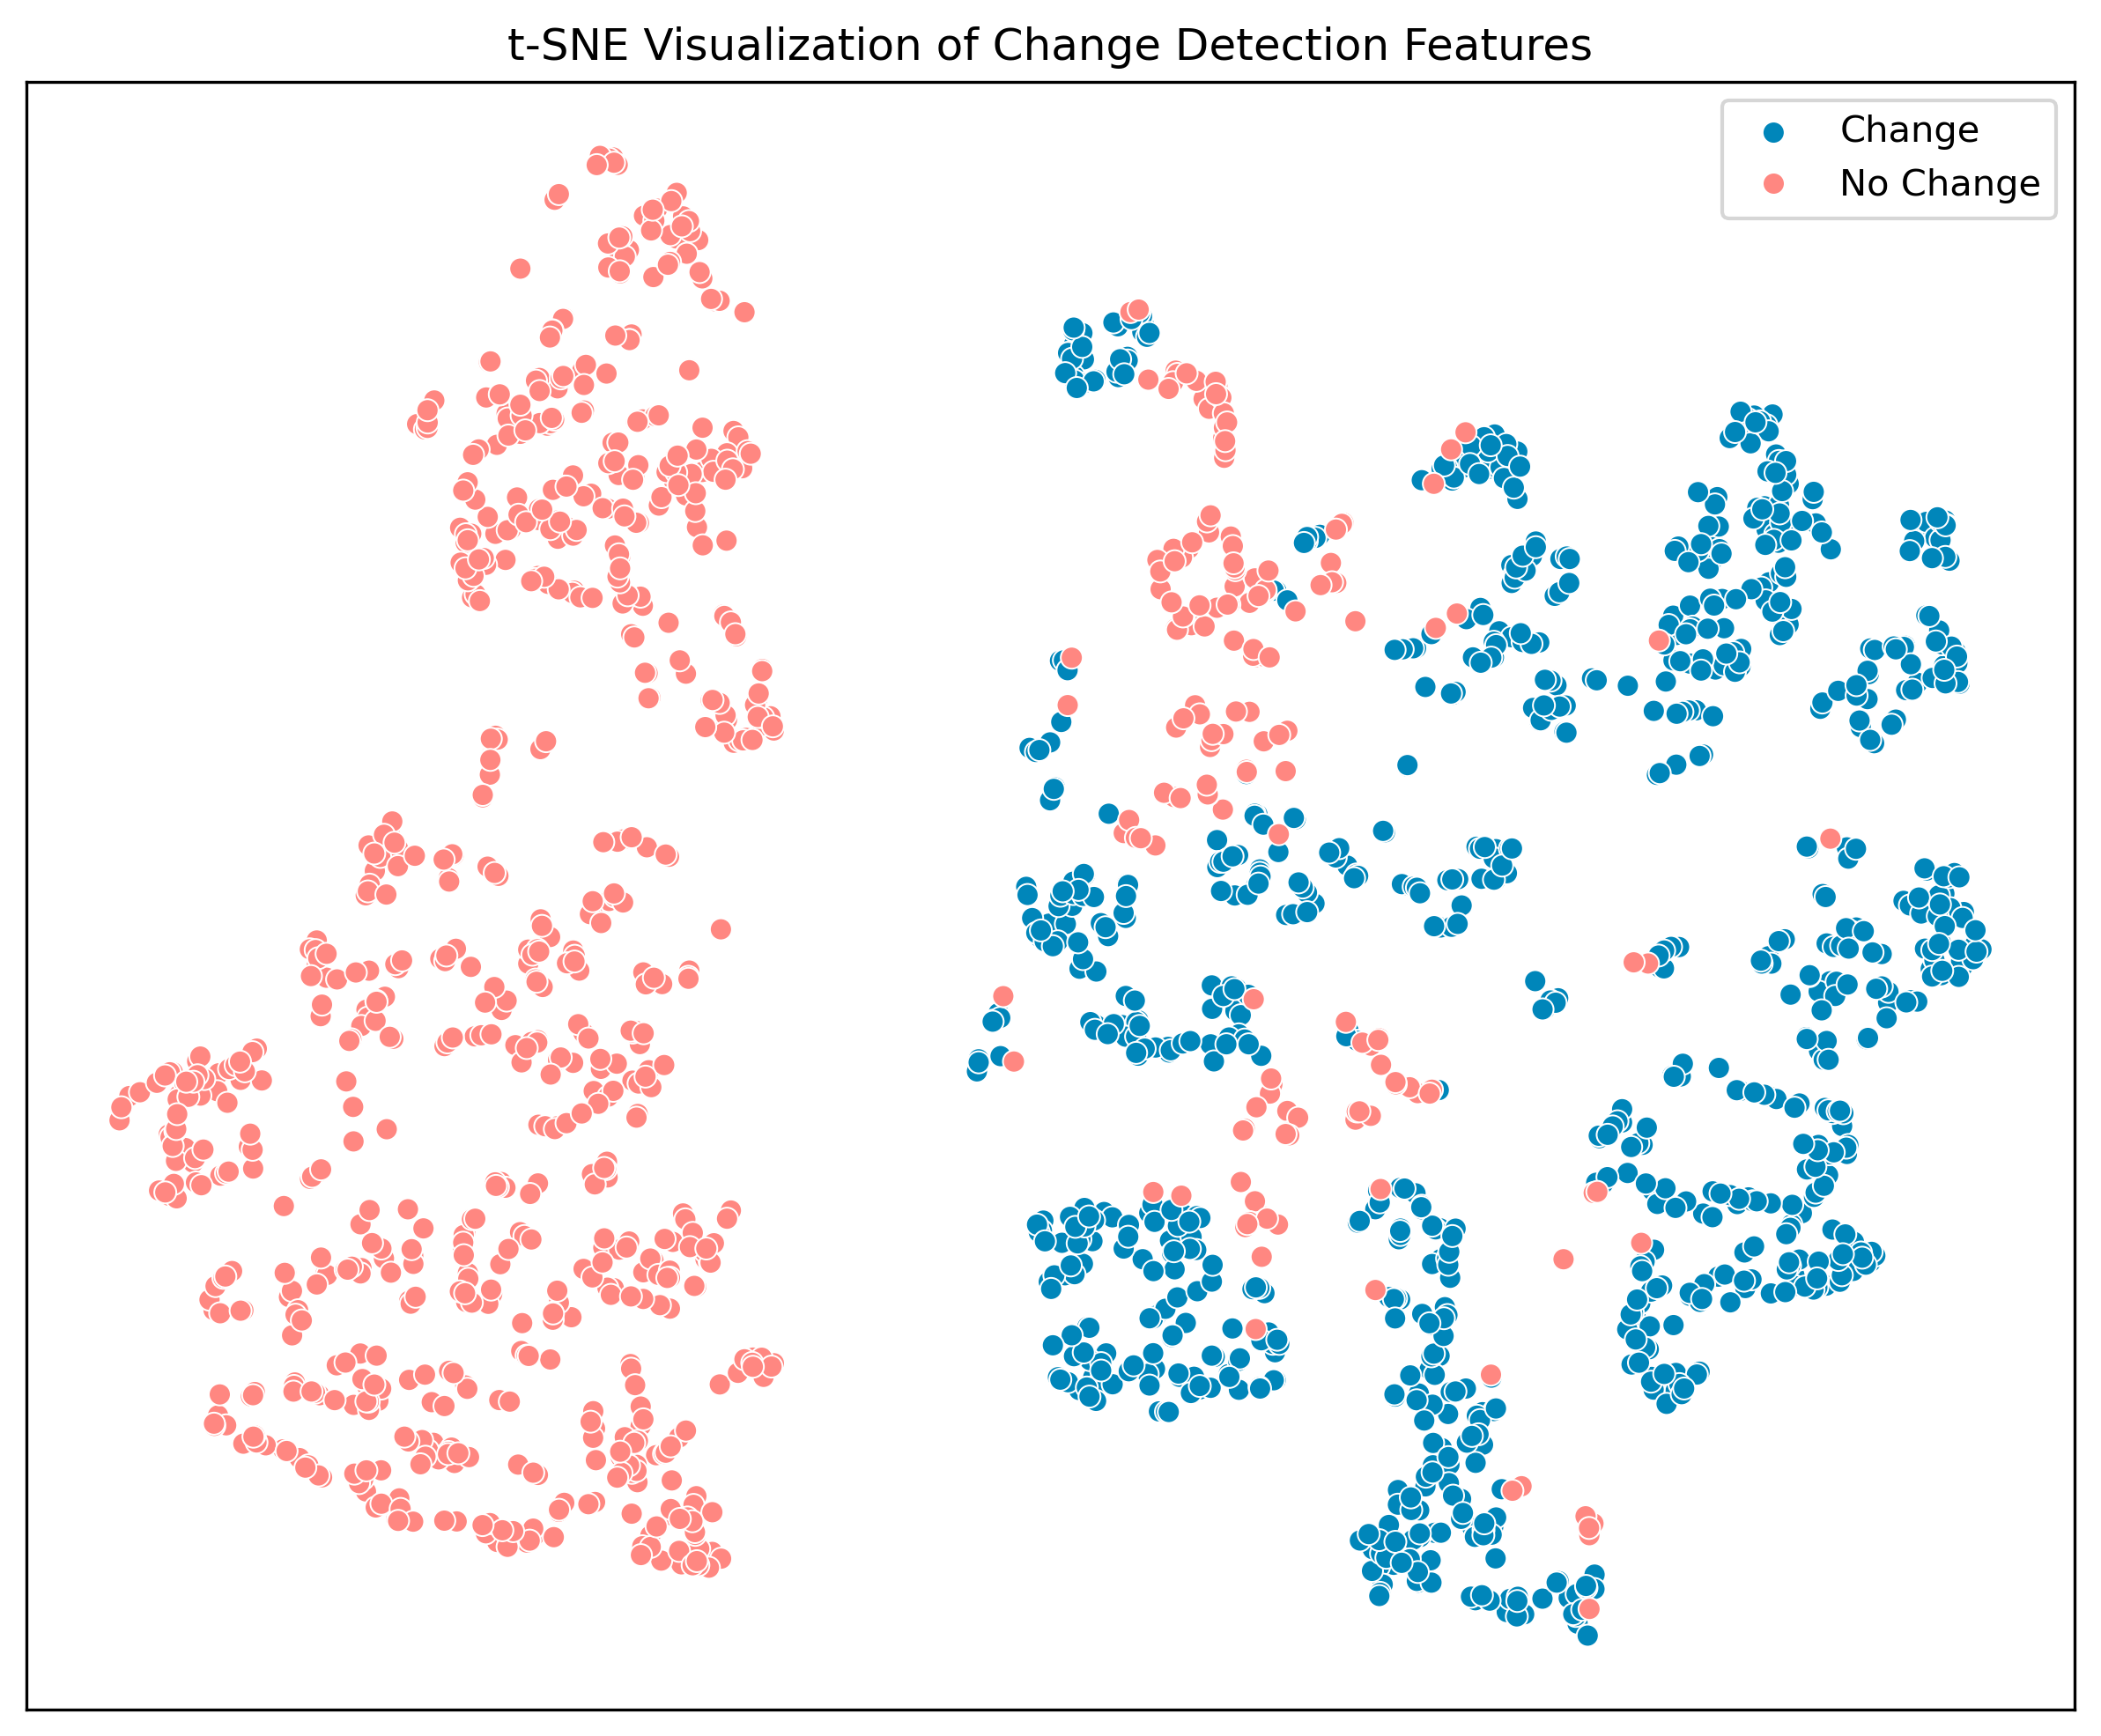
\includegraphics[scale=0.36]{images/tsne_5RCRw.png}
      \caption{RCR随机扰动}
      \label{fig:tsneW_left}
  \end{subfigure}
  \hfill % 两图之间留空
  \begin{subfigure}[t]{0.46\textwidth} % 右图占45%宽度
      \centering
      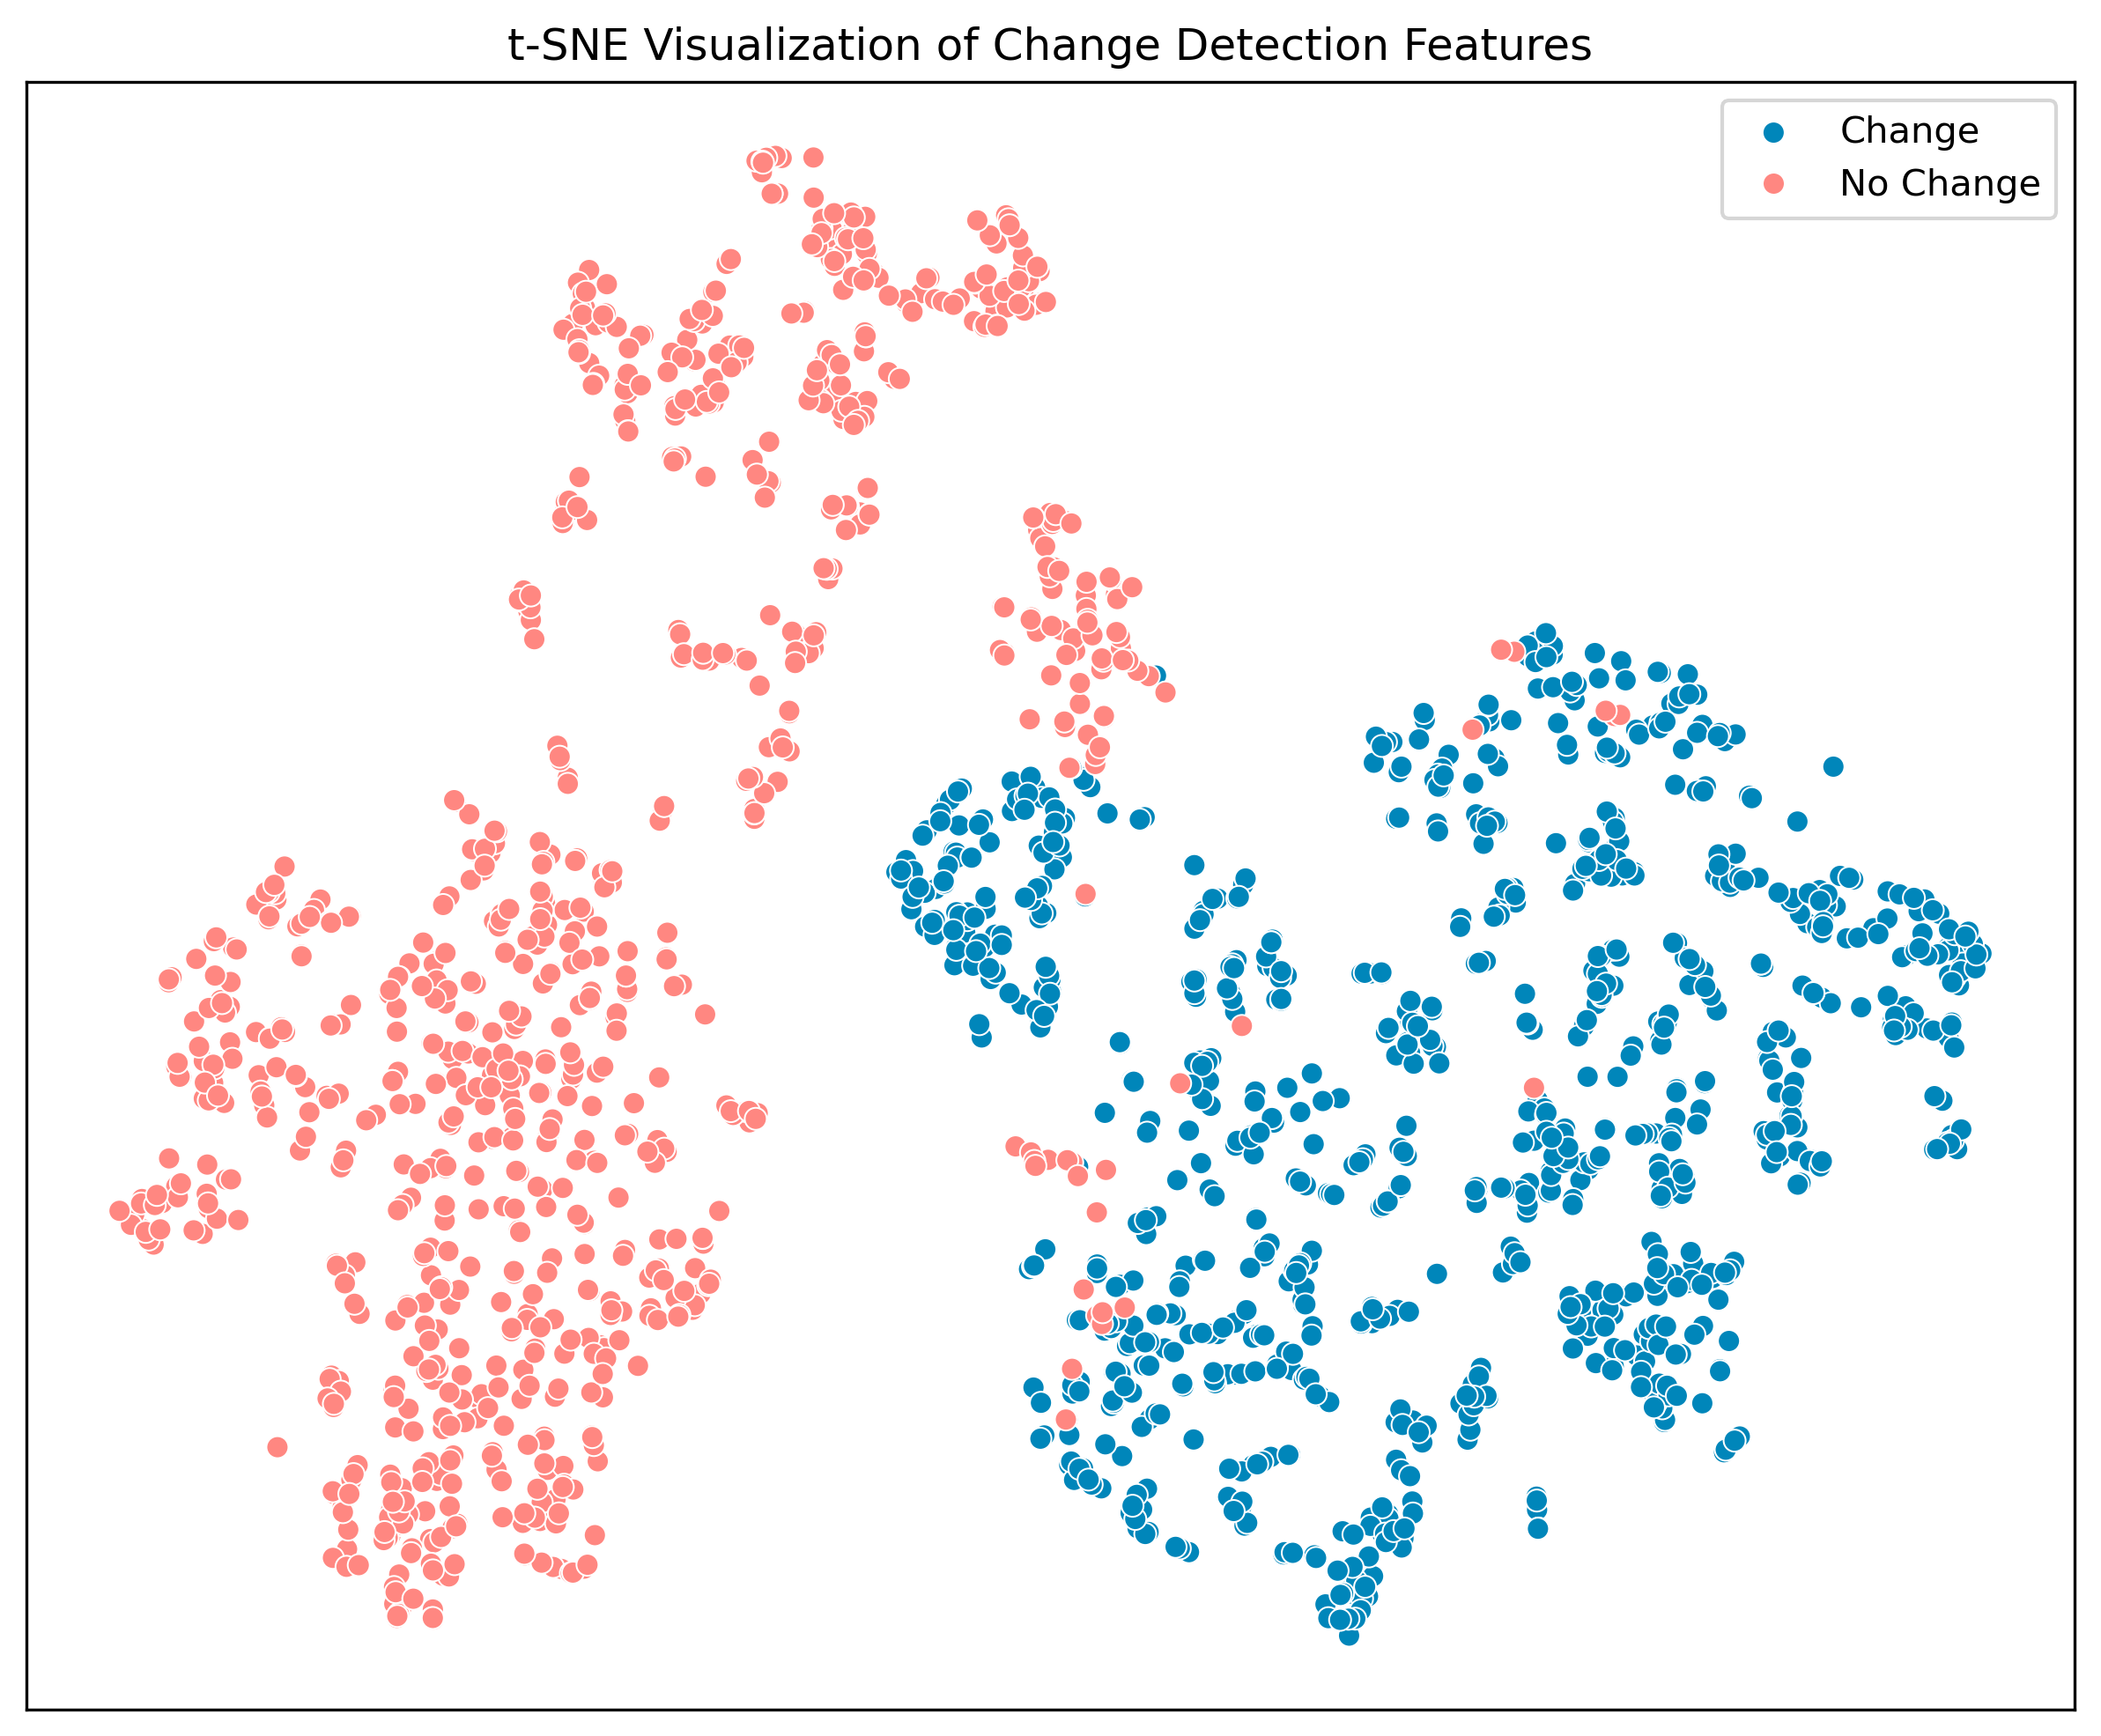
\includegraphics[scale=0.36]{images/tsne_5AdPw.png} % 替换为右图路径
      \caption{AdPSemiCD自适应扰动} % 修改为右图的标题
      \label{fig:tsneW_right}
  \end{subfigure}
  \hspace*{\fill} % 左侧留空
  \caption{WHU-CD测试集上的t-SNE特征可视化对比}
  \label{fig:AdP_tsneW}
\end{figure}
\begin{figure}[H]
  \centering
  \hspace*{\fill} % 左侧留空
  \begin{subfigure}[t]{0.46\textwidth} % 左图占45%宽度
      \centering
      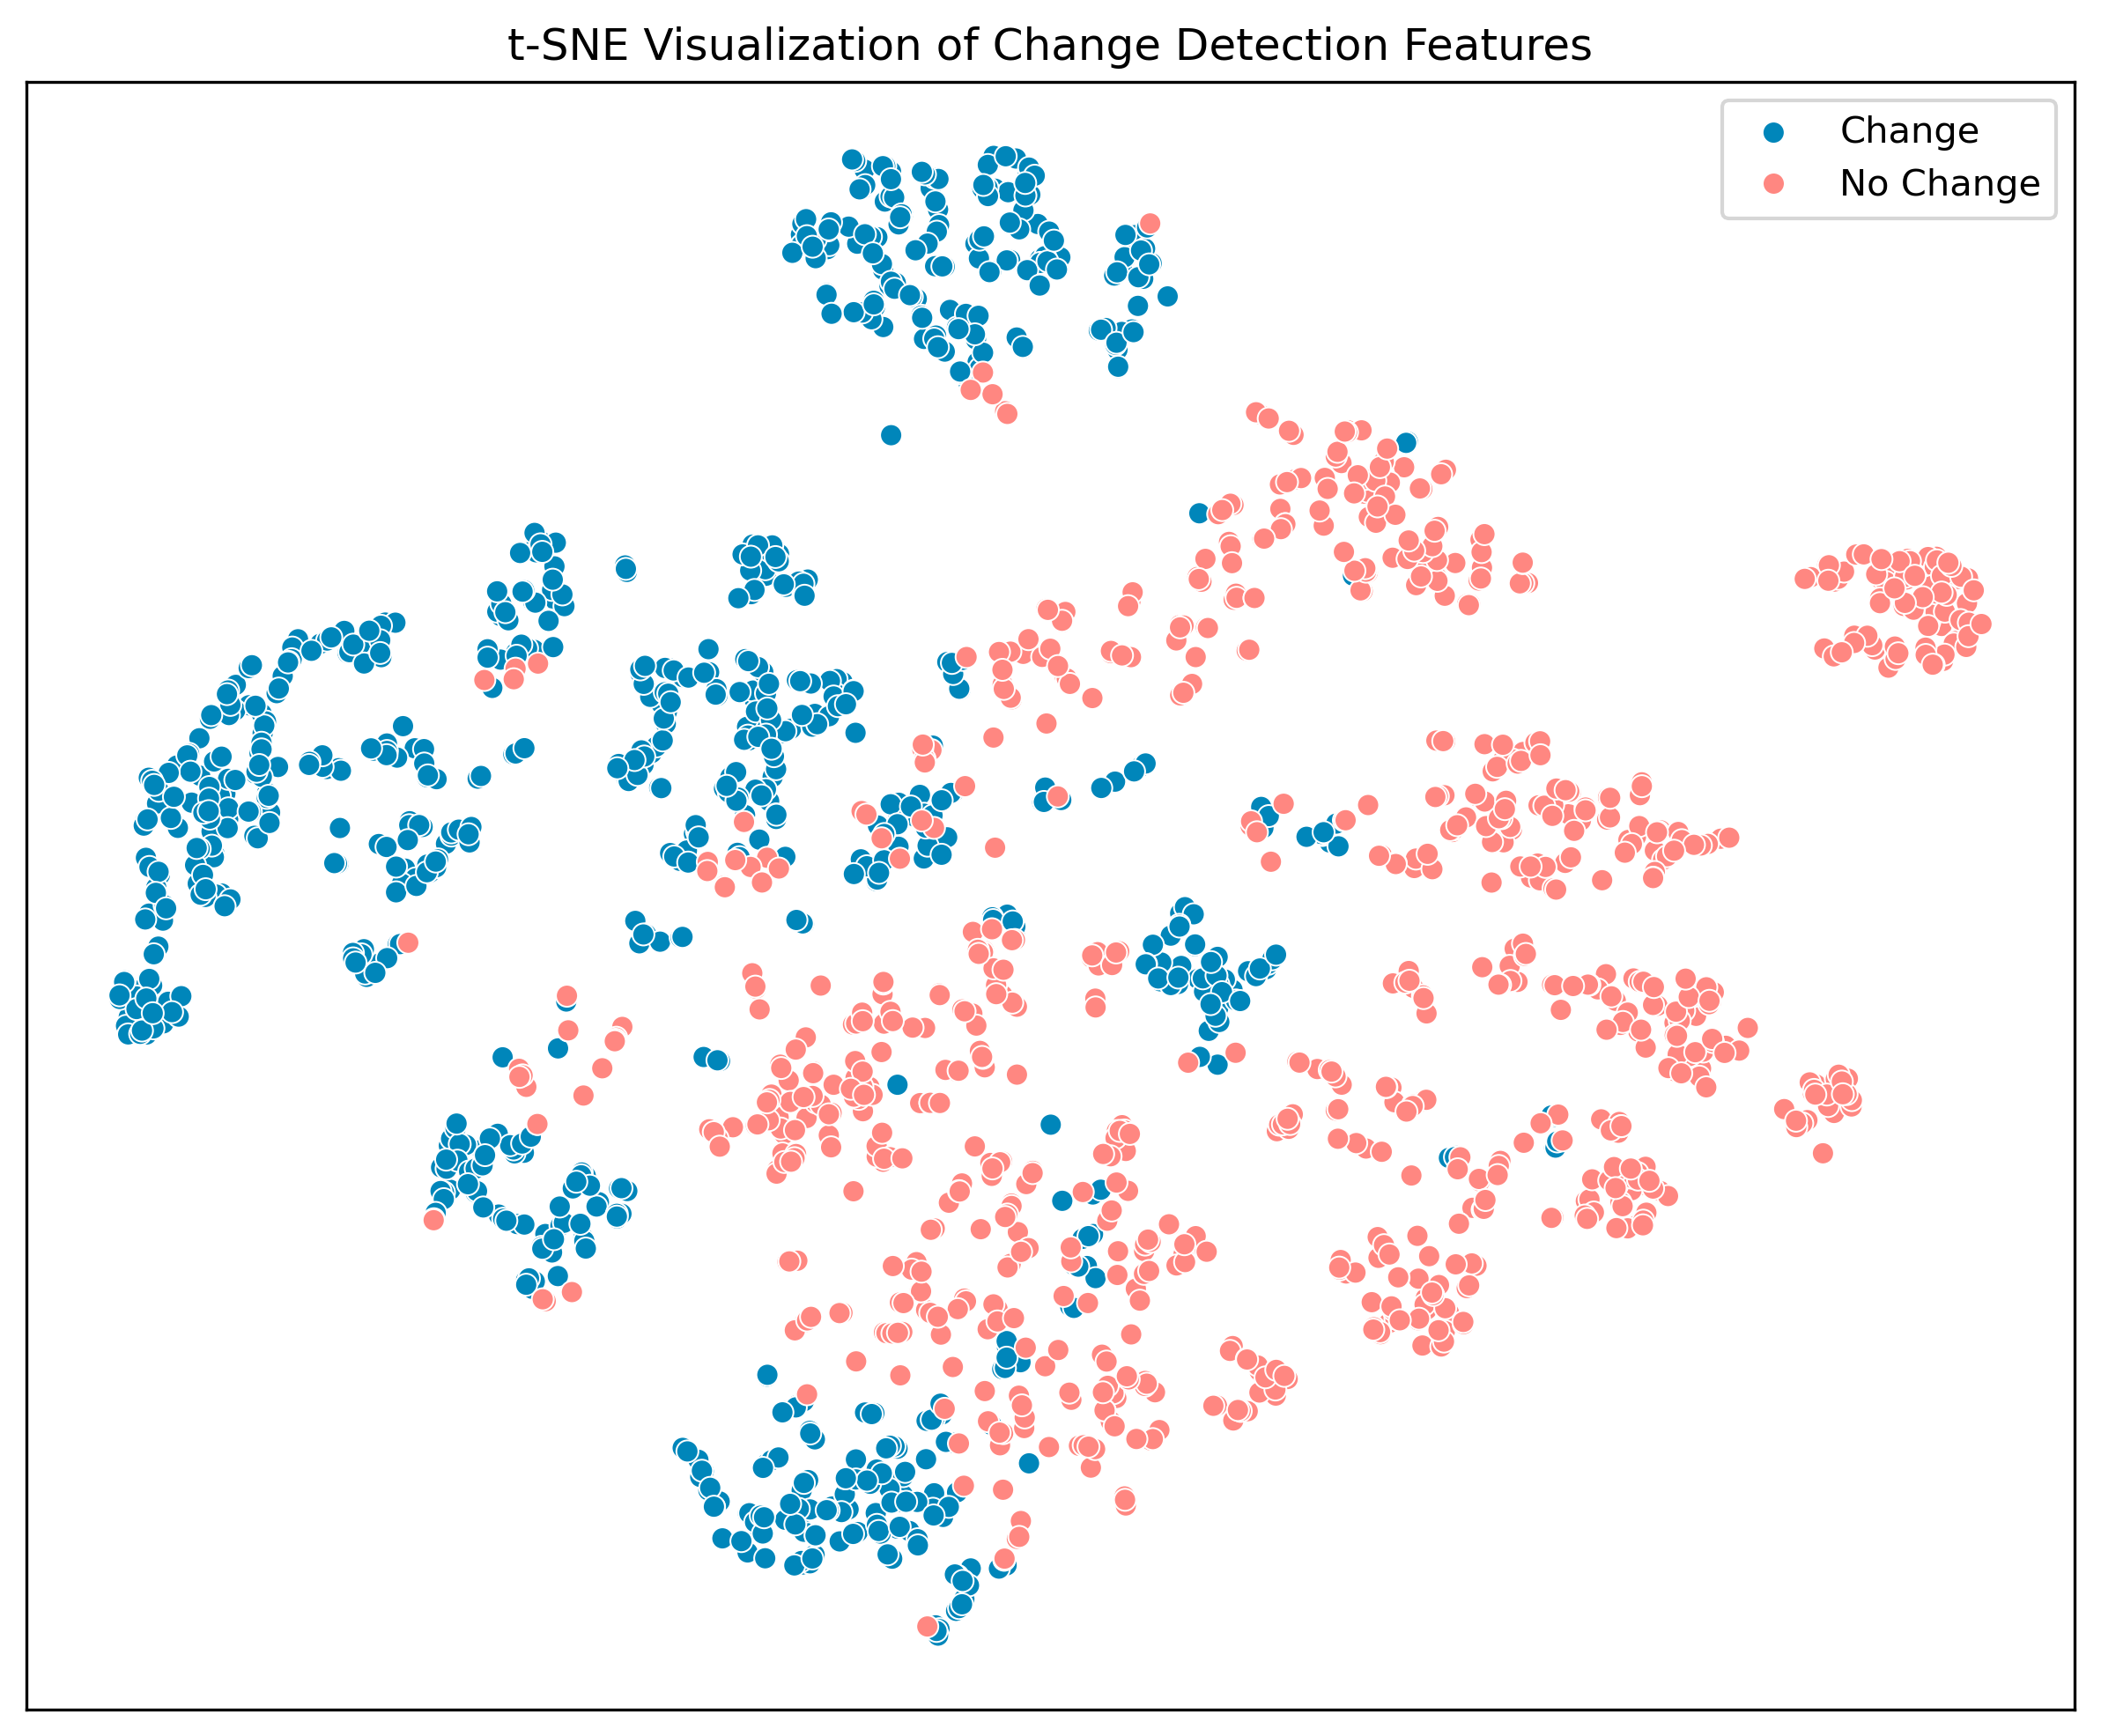
\includegraphics[scale=0.36]{images/tsne_5RCRc.png}
      \caption{RCR随机扰动}
      \label{fig:tsneC_left}
  \end{subfigure}
  \hfill % 两图之间留空
  \begin{subfigure}[t]{0.46\textwidth} % 右图占45%宽度
      \centering
      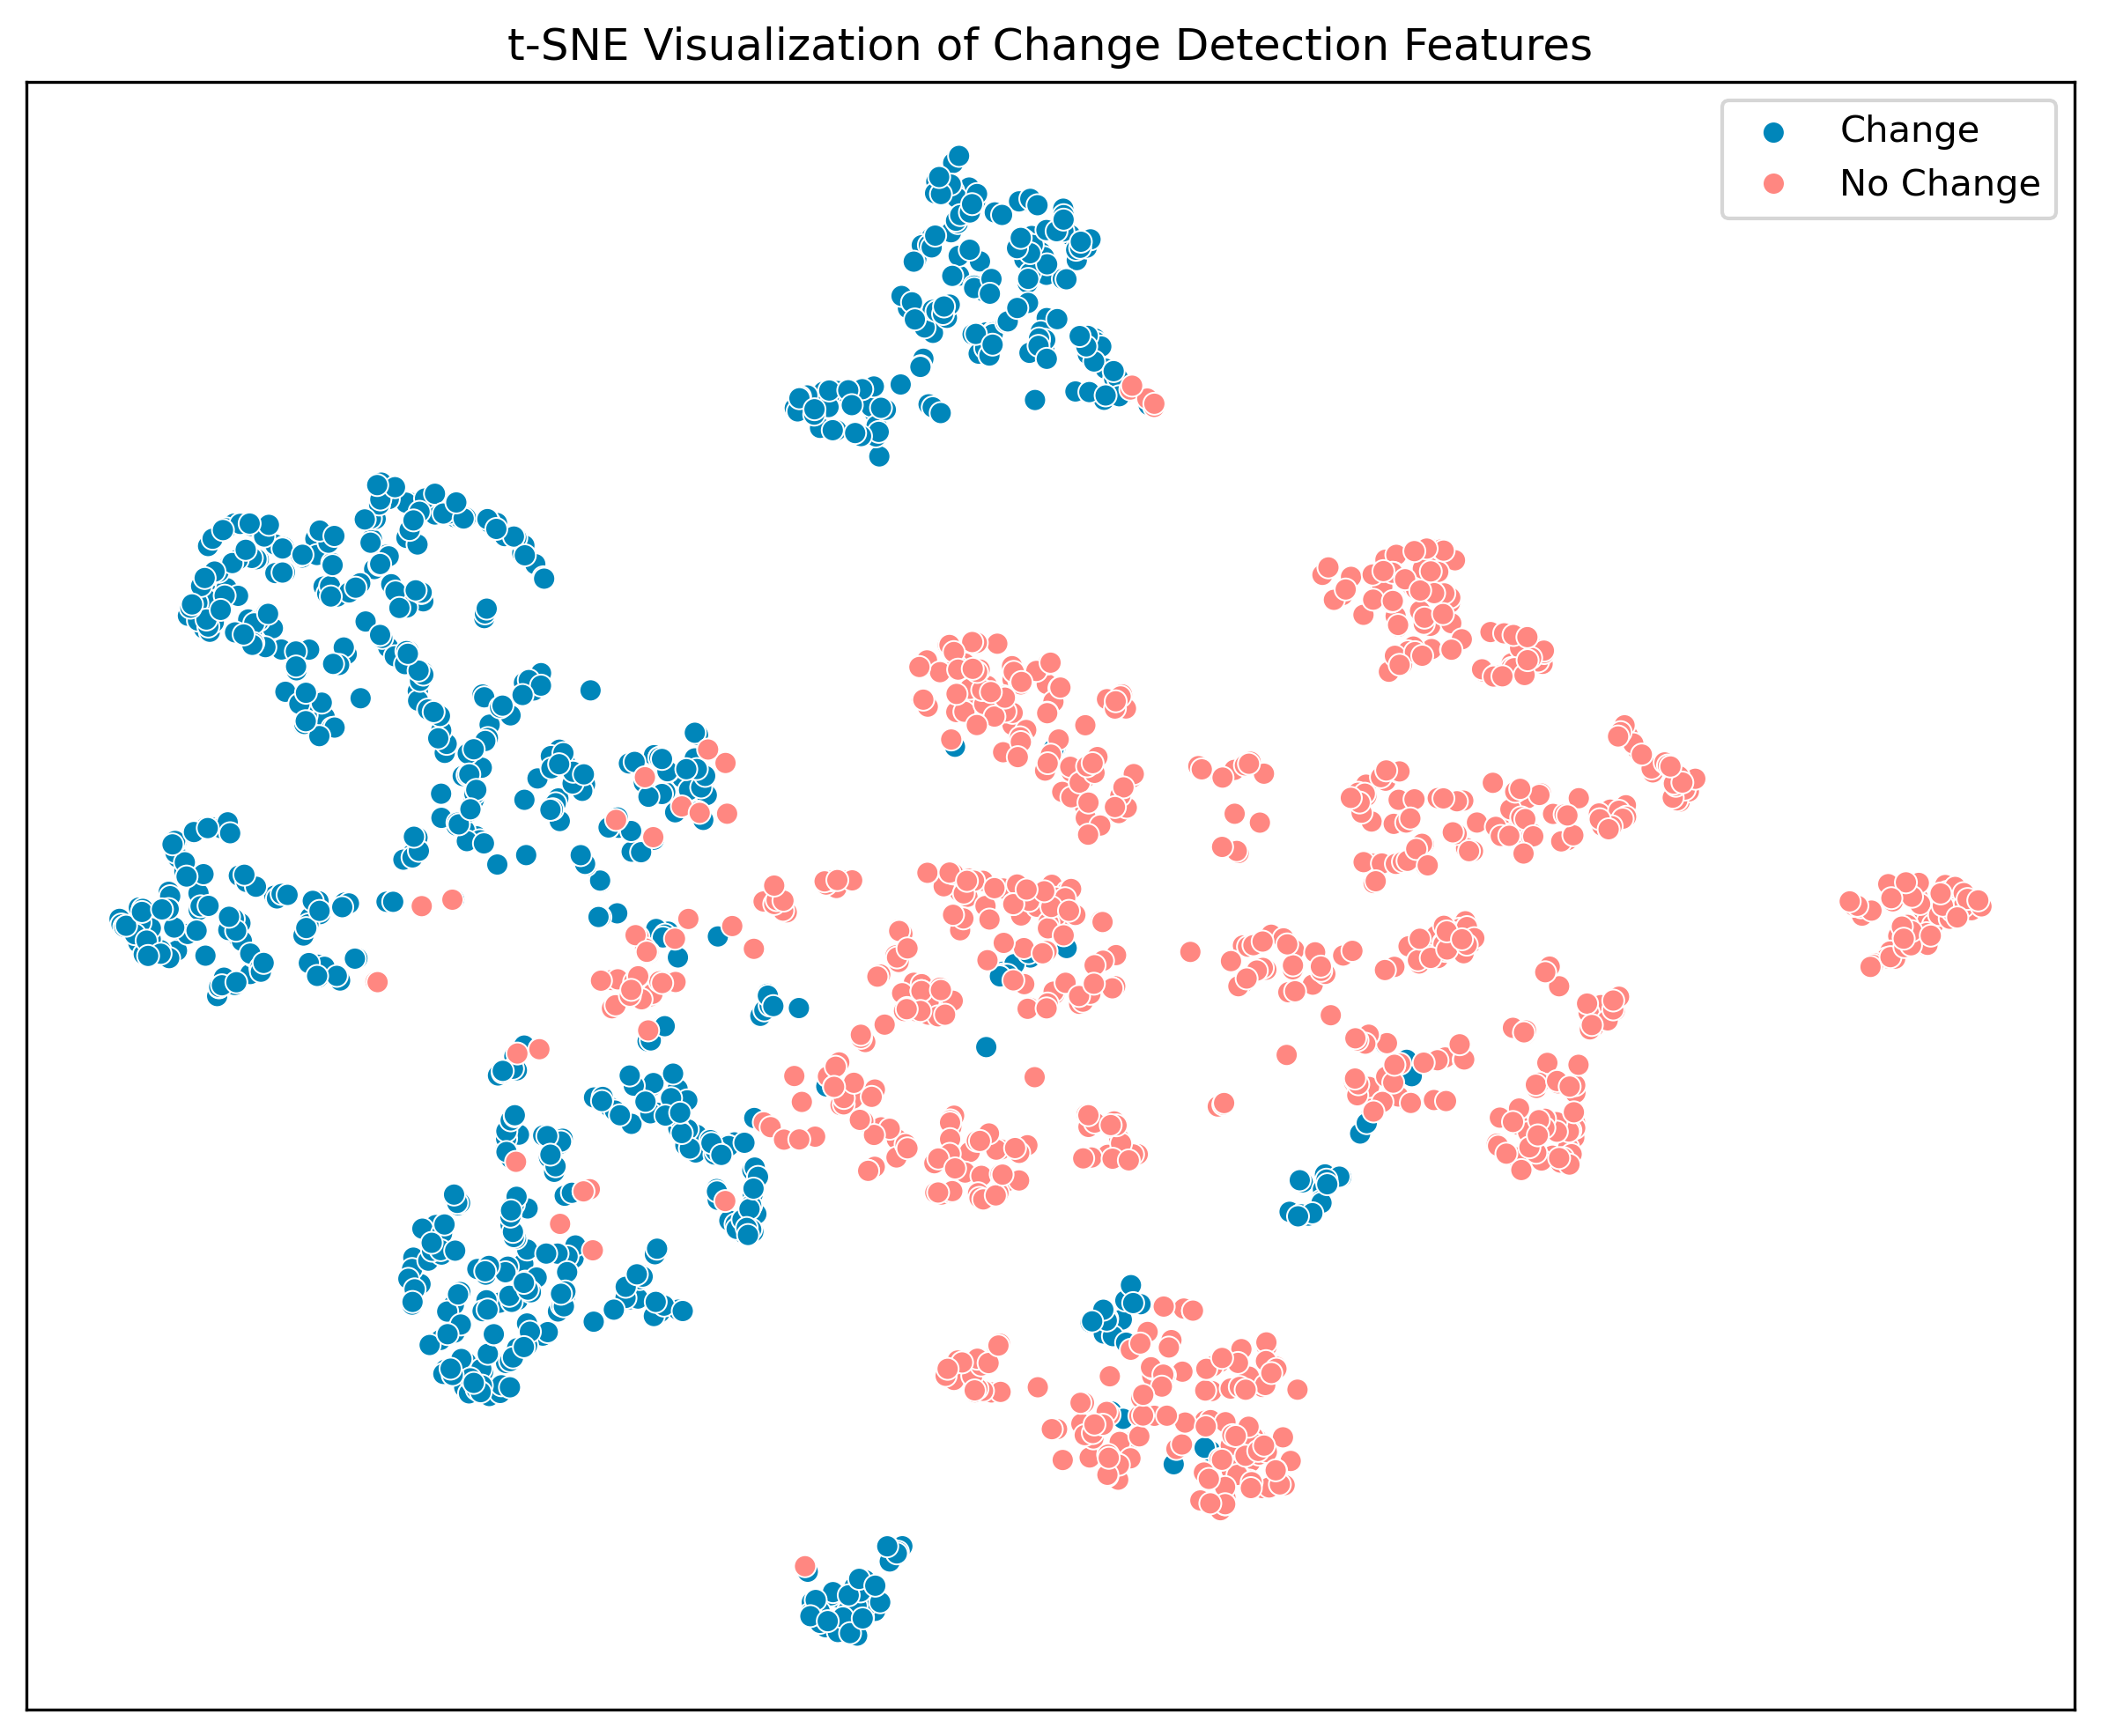
\includegraphics[scale=0.36]{images/tsne_5AdPc.png} % 替换为右图路径
      \caption{AdPSemiCD自适应扰动} % 修改为右图的标题
      \label{fig:tsneC_right}
  \end{subfigure}
  \hspace*{\fill} % 左侧留空
  \caption{CDD测试集上的t-SNE特征可视化对比}
  \label{fig:AdP_tsneC}
\end{figure}
\begin{figure}[H]
  \centering
  \hspace*{\fill} % 左侧留空
  \begin{subfigure}[t]{0.46\textwidth} % 左图占45%宽度
      \centering
      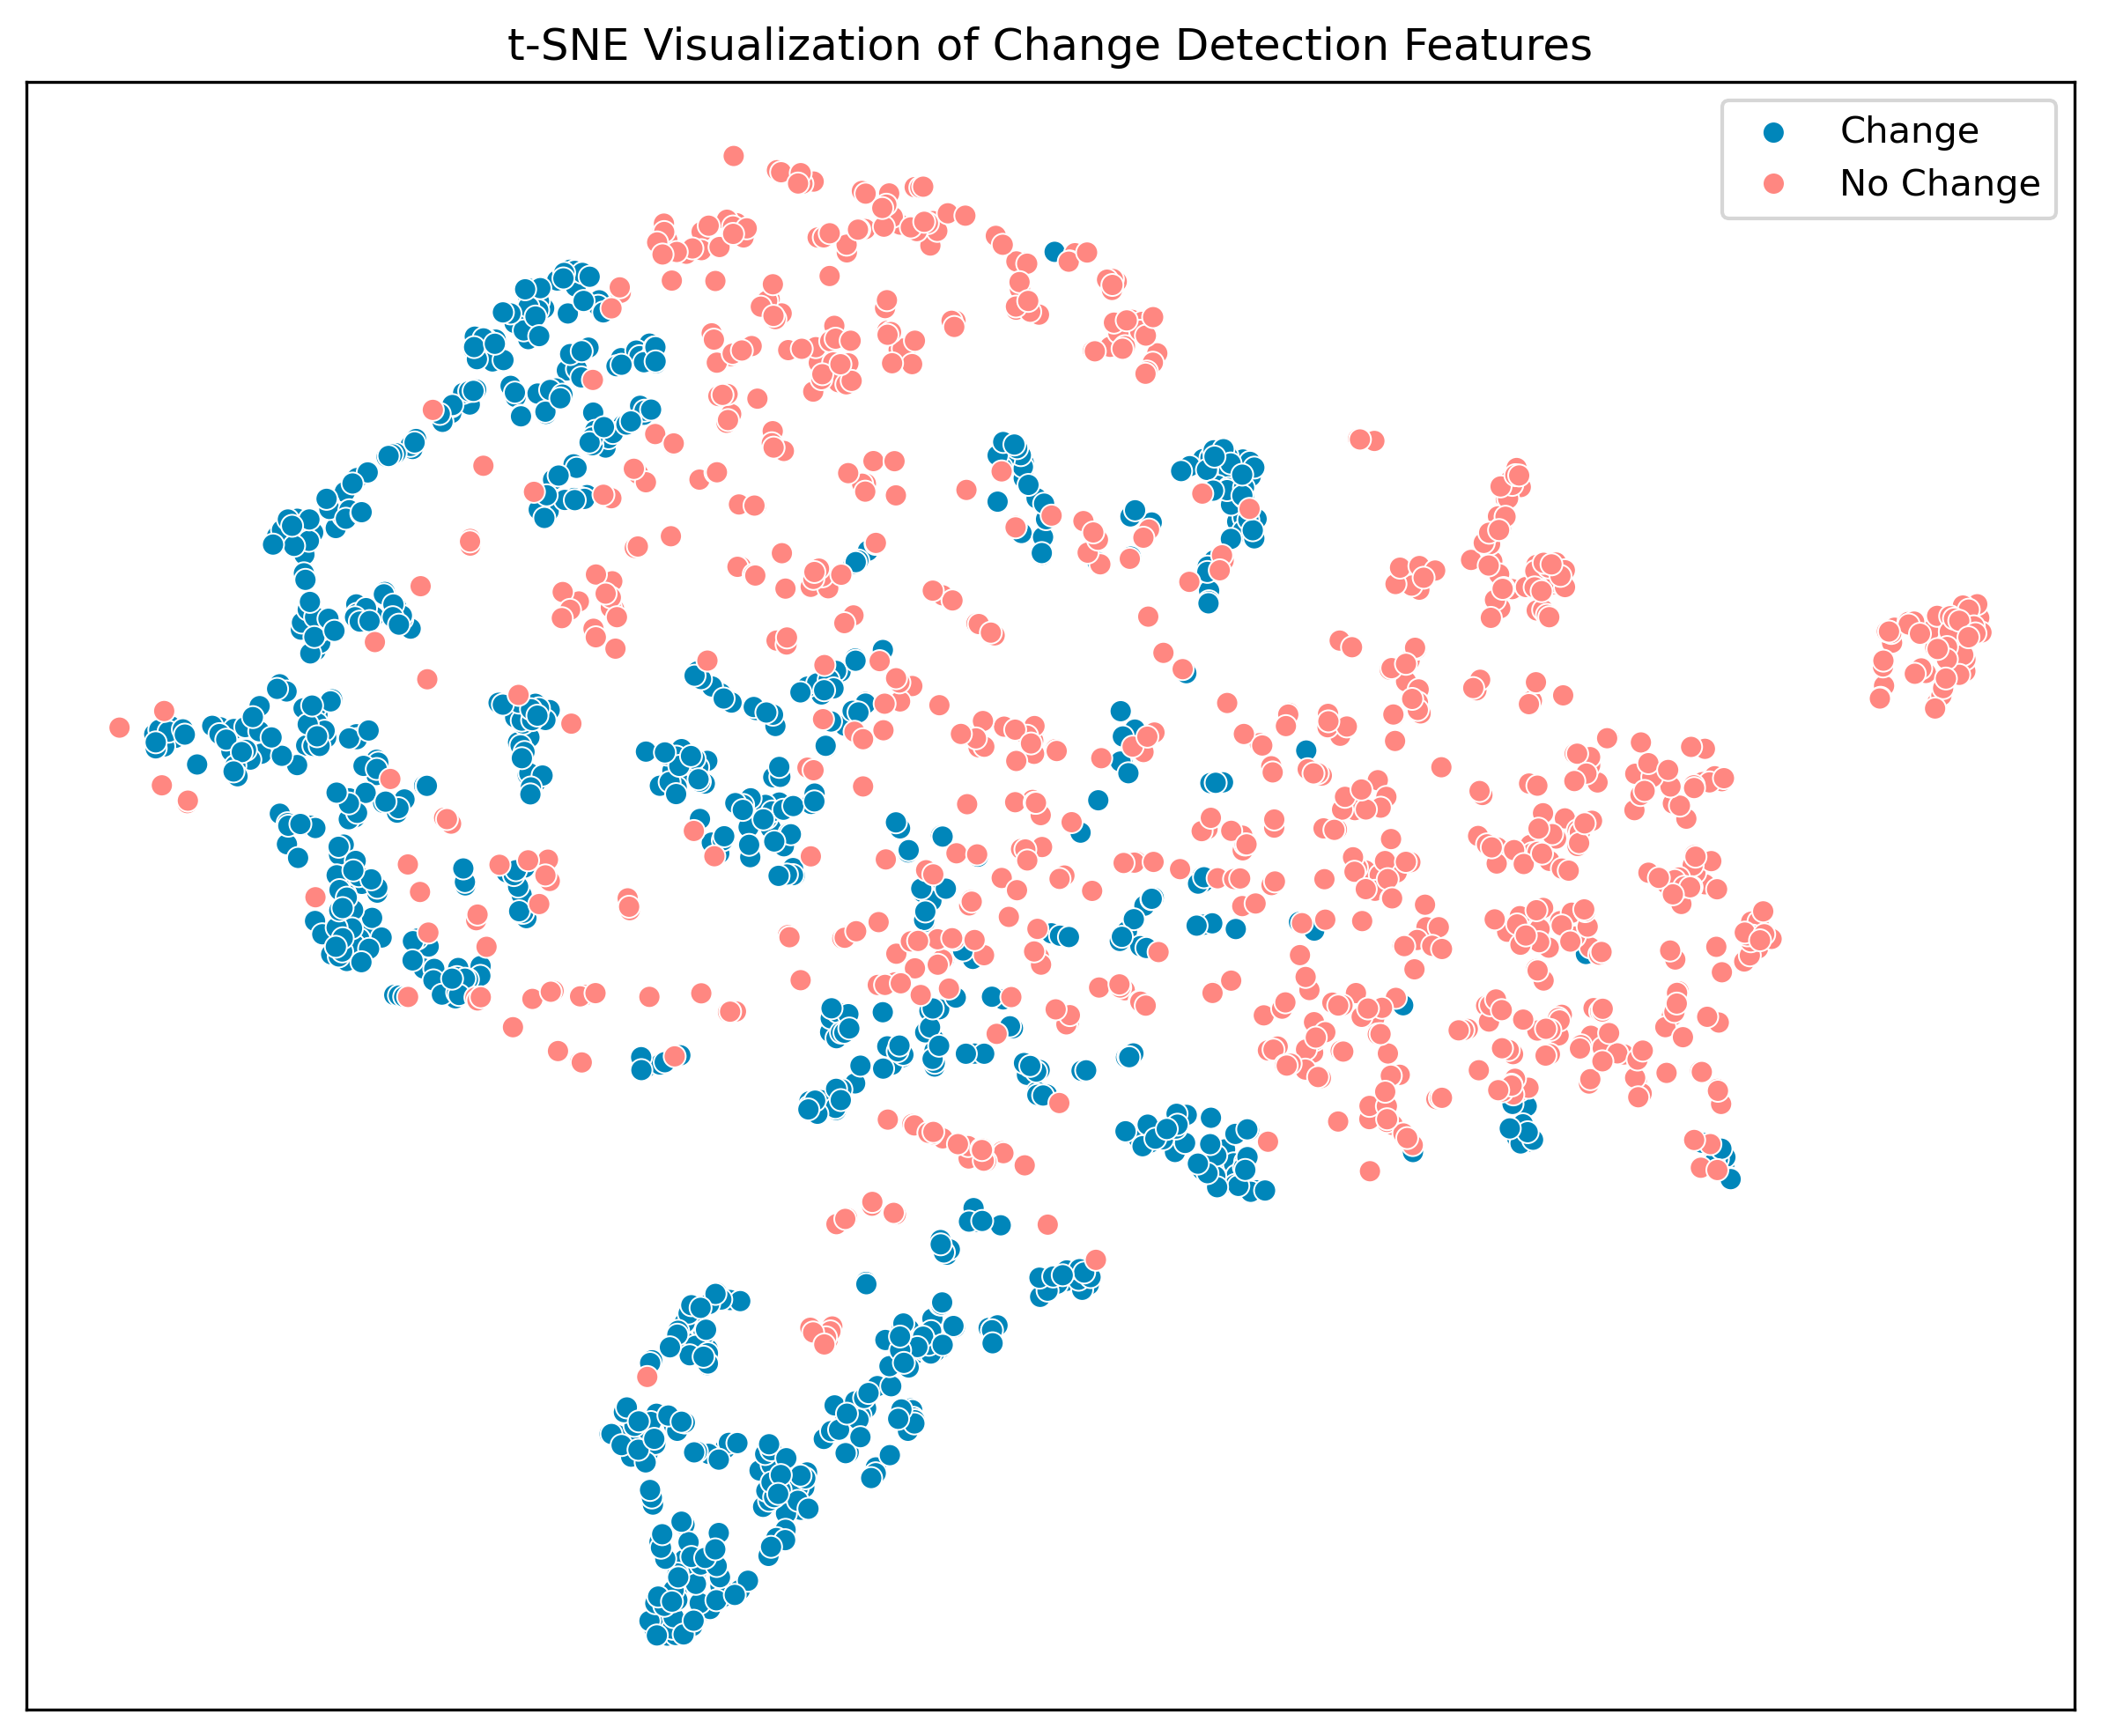
\includegraphics[scale=0.36]{images/tsne_5RCRCl.png}
      \caption{RCR随机扰动}
      \label{fig:tsneCL_left}
  \end{subfigure}
  \hfill % 两图之间留空
  \begin{subfigure}[t]{0.46\textwidth} % 右图占45%宽度
      \centering
      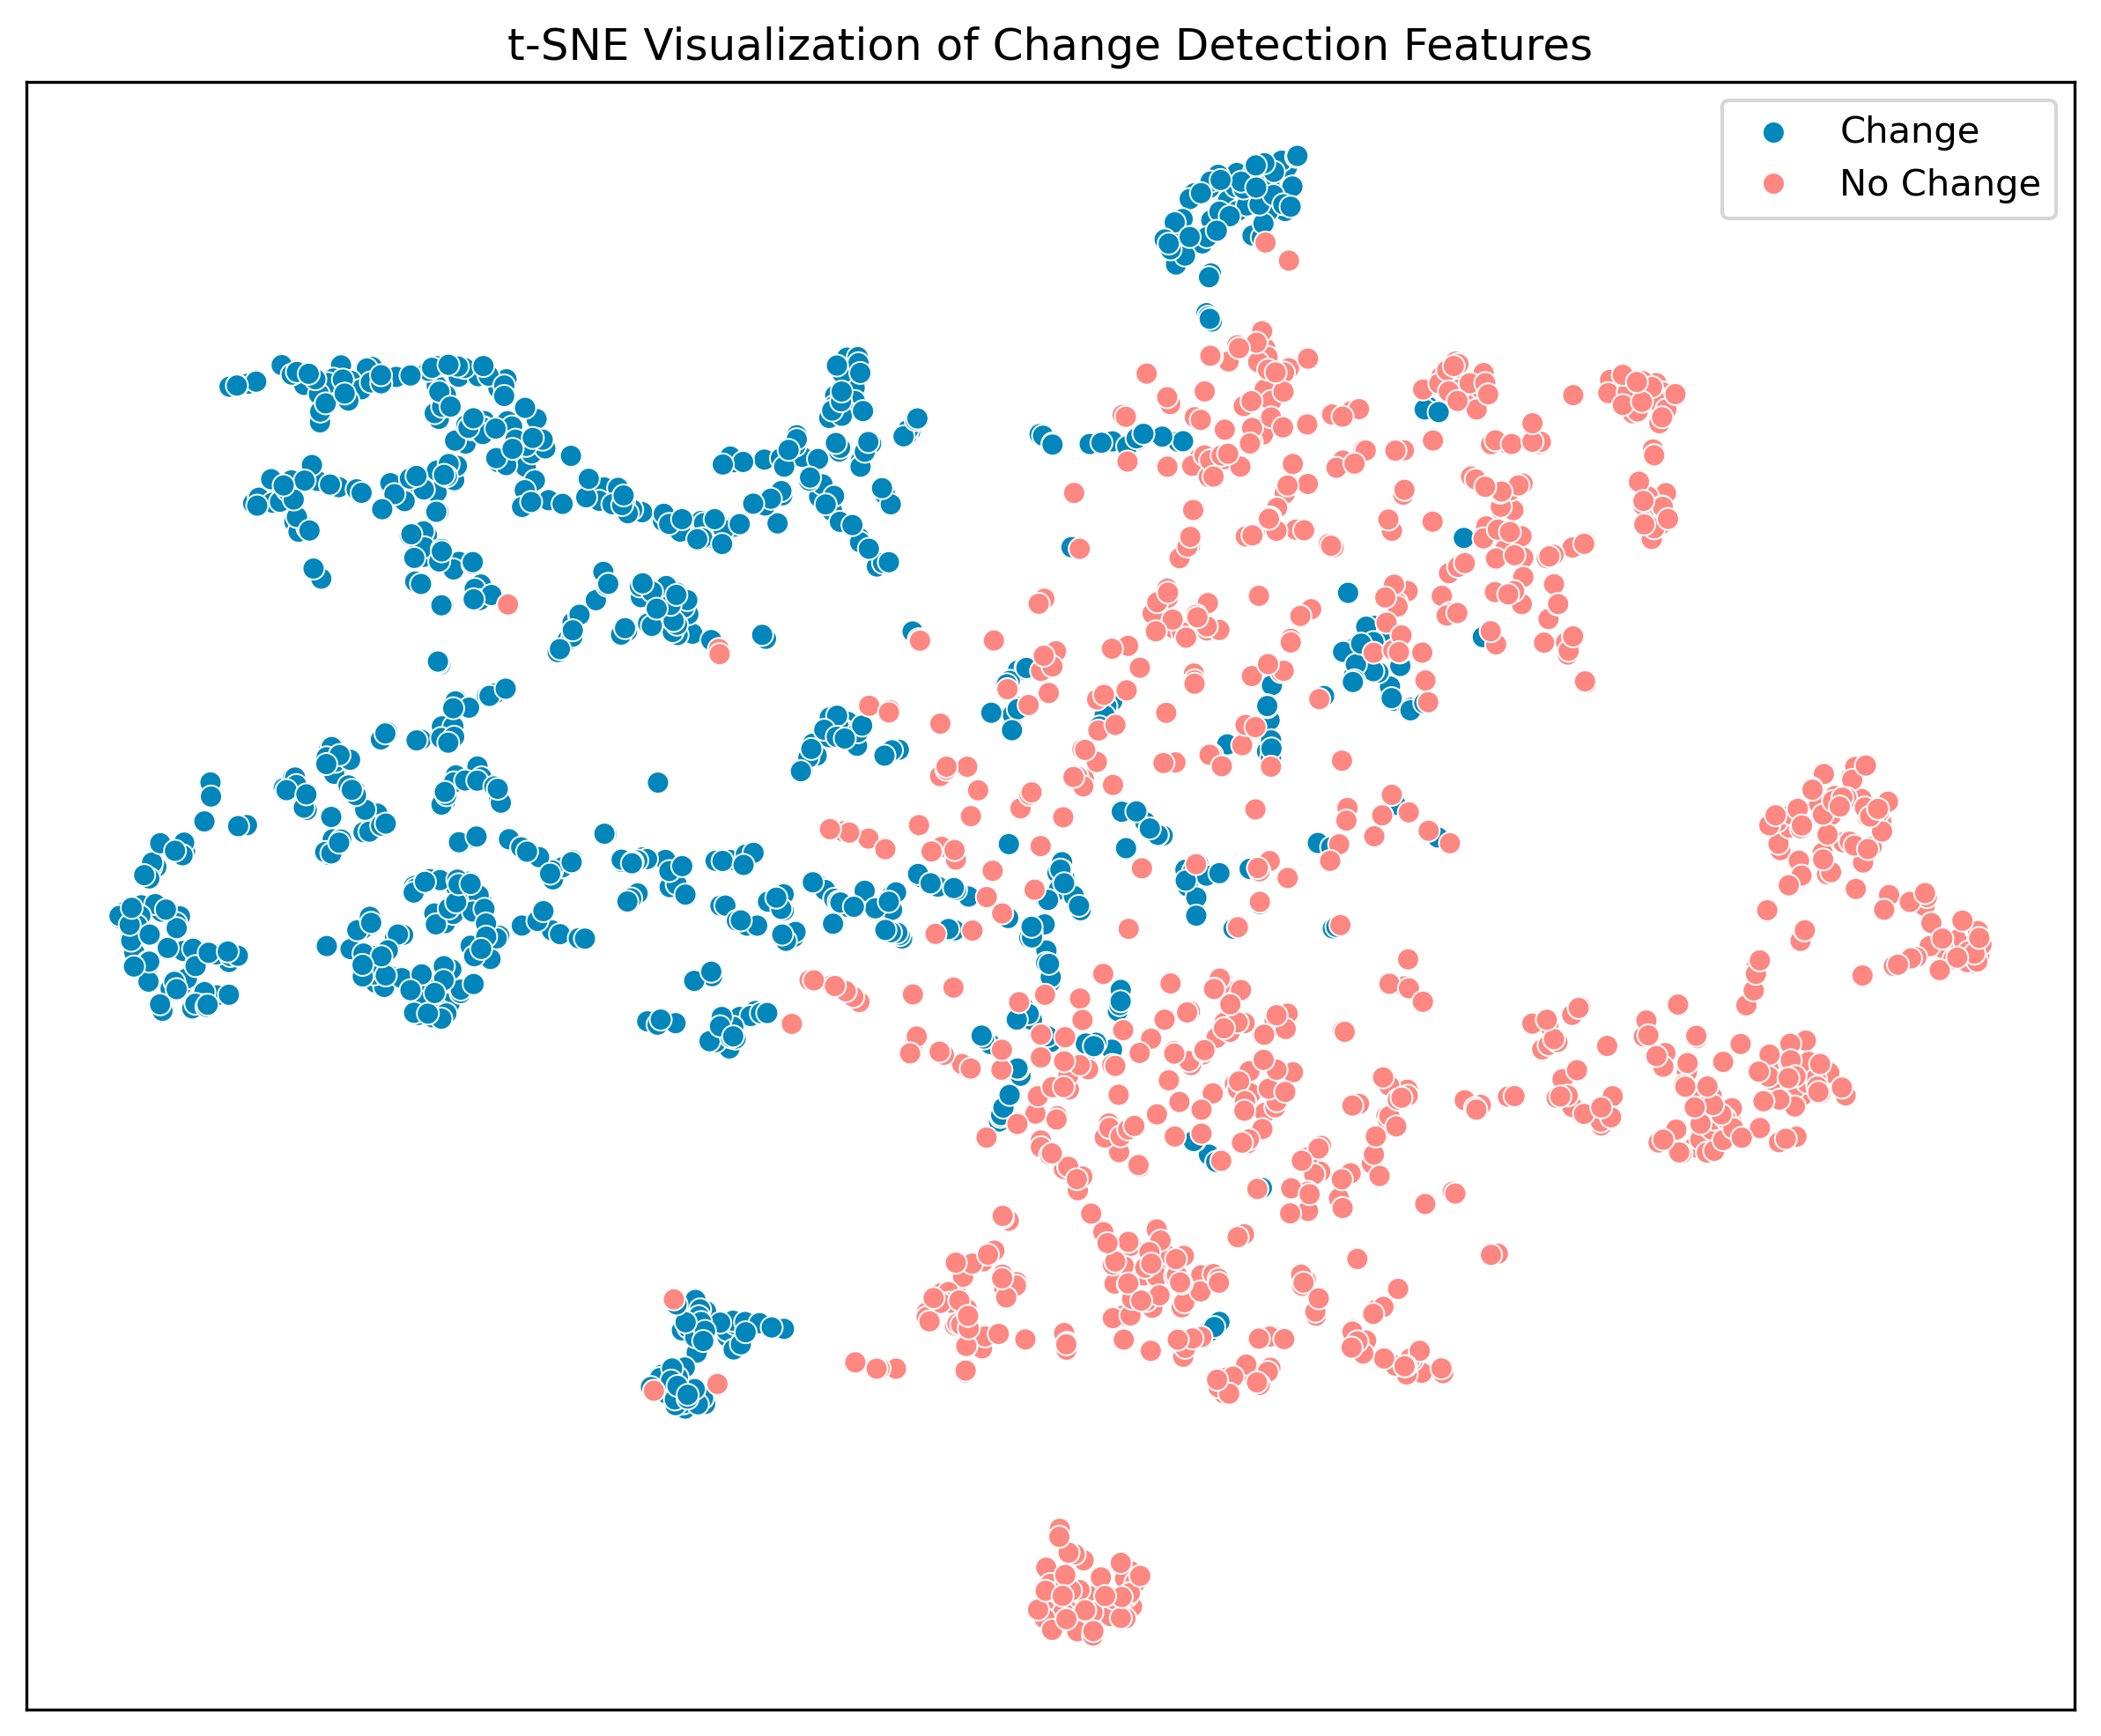
\includegraphics[scale=0.36]{images/tsne_5AdPCl.png} % 替换为右图路径
      \caption{AdPSemiCD自适应扰动} % 修改为右图的标题
      \label{fig:tsneCL_right}
  \end{subfigure}
  \hspace*{\fill} % 左侧留空
  \caption{CL-CD测试集上的t-SNE特征可视化对比}
  \label{fig:AdP_tsneCL}
\end{figure}
相比RCR中使用的随机扰动,使用自适应特征扰动的半监督方法,提取的特征空间中决策边界更加明显,变化前景和背景类别的特征在类内更加紧凑,类间更加分散,直观地验证了自适应扰动方法的优越性。
\section{本章小结}
本章提出了基于自适应特征扰动的半监督变化检测算法,首先在引言分析了此前基于一致性正则化和自训练的半监督方法存在的局限,针对伪标签不够准确和随机扰动方法可能加大确认偏差的问题,我们设计了自适应特征扰动的一致性方法。基于对模型在样本上的预测评估来把握模型的学习状态和样本的难易程度,从而对样本进行自适应的特征扰动,包括自适应选择扰动数量和扰动方式的参数自适应缩放。最后展示了我们在十个数据集上的对比实验和消融实验结果,从定量的实验指标和定性的可视化结果,全方位地证明了本章所提出的AdPSemiCD的有效性。
\cleardoublepage
\chapter{总结与展望}
\section{本文工作总结}
变化检测是遥感影像自动解译领域的一个重要研究方向,在许多领域发挥着重要作用,例如,城市建设规划、森林环境保护、农村土地管理、自然灾害评估等。针对变化检测任务的数据标注非常复杂,耗时耗力。而在如今非常成熟的对地观测技术之下,无标注的数据相对来说容易获得。因此本文通过半监督学习的方法将大量的无标注样本利用起来,使得模型仅需少量的人工标注即可达到可观的检测效果,解决了基于深度学习的变化检测方法对标注训练数据的依赖问题,提高了变化检测在实际应用场景中的可行性。

本文首先综述了变化检测任务的发展历程,梳理了国内外关于半监督变化检测的相关研究现状以及半监督学习的主要途径和方法,并对卷积神经网络和此前的最佳半监督变化检测算法进行了详细介绍。最后本文着力研究了基于伪标签自训练和一致性正则化的半监督变化检测,主要从伪标签阈值、伪标签改造以及扰动一致性三个角度设计了半监督变化检测算法。本文的主要研究内容如下:

    1)针对当前基于伪标签和一致性正则化的方法中,采用固定阈值或特定阈值调整策略可能无法充分利用未标记数据的局限性,我们提出了一种基于自适应动态阈值的半监督变化检测算法——AdTSemiCD。该算法通过监测模型预测的置信度动态把握其学习状态,并据此实时调整伪标签的阈值。此外,为了充分挖掘被筛选掉的低置信度标签所包含的潜在信息,我们设计了一个低置信度学习模块,从而进一步提升训练效率。实验结果表明,所提方法减少了在某些稀少样本类别上的漏检问题,表现除了优越的性能。

    2)针对模型生成的伪标签在不同难度无标记样本上存在噪声差异,同时对模型训练的贡献度也不均衡的问题,我们提出了一种基于伪标签评估的自适应半监督变化检测算法——AdaSemiCD。首先,我们设计了AdaFusion模块,用于在单样本层面改造高不确定性区域,显著提高伪标签的准确性。其次,我们提出了AdaEMA模块,在模型参数更新过程中引入自适应选择机制,使模型能够更有效地整合优化参数。大量实验验证了该方法显著改善了伪标签质量,从而有效提升了变化检测的整体性能。

    3)针对现有一致性正则化方法在对所有样本采取相同扰动策略时可能扩大模型确认偏差的问题,以及基于硬伪标签的自训练方法中不可避免的噪声问题,我们提出了一种基于自适应特征扰动的半监督变化检测算法——AdPSemiCD。该方法通过对无标记样本的预测结果进行评估,针对难易程度不同的样本特征自适应地施加扰动,具体包括对扰动数量和扰动强度的动态选择。通过这种样本级定制的扰动策略,算法在扩展特征空间和减少确认偏差之间达到了平衡,从而为模型训练提供了更有效的一致性约束。最终,实验结果充分验证了该自适应特征扰动策略的有效性和实用性。
\section{未来研究展望}
本文对半监督遥感影像变化检测算法进行了全面、系统的调研,并分别从伪标签筛选、伪标签改造以及特征空间优化三个层面进行了改进。然而,目前还有一些工作值得继续深入探讨研究:

1)当前基于伪标签自训练的半监督变化检测算法,都依赖于为无标记样本生成的高可信伪标签,伪标签质量直接影响模型的学习效果。但是仅仅依靠仅有少量真实标签训练的模型自身来生成伪标签是存在瓶颈的,除了在伪标签筛选、伪标签改造两个阶段进行一些处理之外,还可以探索在伪标签生成网络层面进行探索,例如引入在大量遥感数据上进行过预训练的大模型来辅助生成伪标签,或许有望突破伪标签质量瓶颈,甚至完全解决半监督变化检测这个问题。

2)积极探索半监督变化检测与多模态学习的融合。半监督学习可以利用大量的无标记样本训练,天然适合将大量的不同模态(例如合成孔径雷达图像、红外图像等)的无标记样本利用起来,互补性地提供信息,以更好地提高模型泛化性,乃至将光学图像变化检测、合成孔径雷达图像变化检测等细分任务统一起来。
\cleardoublepage
%%=============================================================================%
%% 参考文献以及附录
%%-----------------------------------------------------------------------------%
%% \bibliographystyle{nputhesis}                               % GB/T 7714-2015 格式
\bibliographystyle{nputhesis-noslash}                       % 参考文献改进格式
\bibliography{reference}                                    % 参考文献
\appendix

%%=============================================================================%
%% 文档附页部分(致谢、参加科研情况、知识产权与原创性声明)
%%-----------------------------------------------------------------------------%
\backmatter                                                 % 文档附页部分
%%-----------------------------------------------------------------------------%
\begin{acknowledgements}                                    % 致谢开始
伴随着此文落笔,我的西工大研究生生活即将画上句号。曾经无比期待这一天的到来,但当它真的来临时,心中却充满了复杂的情感。都说读研只有录取和毕业是最开心的时刻,但当我回首这几年,发现一路走来,我收获的不仅是知识,更是无数值得铭记的瞬间。还记得,犹记得刚来到这里的第一天,无比迷茫的我在夜晚骑车一圈圈地环绕校园,借着路灯的微光,仿佛找到了前行的方向。但其实,那灯光不过是心灵的寄托,帮助我走出自己的误区,与自己和解;真正指引我不断前行的,是我的导师、同门、朋友和家人。他们的陪伴和支持让我克服困惑,跨越难关,沿着正确的道路坚定向前。对此,我怀着深深的感激之情,铭记于心。

我要感谢我的导师冉令燕老师。冉老师和蔼可亲,虽为师生,却更像朋友,彼此尊重、互相关怀。冉老师时常关心我们,流行病期间提醒大家注意健康,逢年过节组织组内聚餐,营造了温馨和谐的实验室氛围。科研上,冉老师治学严谨,责任感强,耐心指导我们读文献、理思路、找创新、做实验和写文章,可以说是我心中理想型导师的典范。感谢您三年来的指导,助我顺利完成学业,也让我度过了一段多年后回想起来仍觉美好的时光。

我要感谢我的同门、师兄师姐、师弟师妹们,在读研期间两点一线的生活中,和大家在实验室的相处时光最多,大家一起在科研上互帮互助、共同进步,以及闲暇时光一起约饭、打羽毛球的这些经历非常值得留恋,感恩遇见你们,为我本来平常的生活增添了色彩,也真诚地祝愿大家都将拥有景绣前程。

我要感谢我的室友和好朋友们,感谢你们的陪伴,一个人固然可以埋头走得很快,但一群人才能够相互扶持走得很远,感谢你们在我生病期间的关心和照顾,以及在很多精神内耗的时间段,愿意成为我倾诉的对象,帮助我走出阴霾。也在此祝福大家此去一路顺利,多年之后归来仍是少年。

最后,我还要感谢我的家人,感谢你们无论是经济上还是情感上的坚定支持,读研这一路走来没有你们的默默支持我是无法心无旁骛、集中精力完成学业的,是你们给了我前进的底气和勇气。我会继续努力,在未来的工作中脚踏实地,用自己的能力回报你们。

同时,我也要感谢在繁忙的科研工作中抽出宝贵时间对我的论文进行评审的专家教授和参加论文答辩的各位老师,衷心地感谢你们在评审和答辩过程中提出的宝贵意见和建议!

“道路是曲折的,前途是光明的”。行文至此,我想以这一句作为结尾,也作为未来生活的勉励。梦虽遥,追则能达;愿虽艰,持则可圆;不怕困难,迎难而上。也祝福我们的党和国家繁荣昌盛,河山添锦绣,星光映万家,早日实现中华民族的伟大复兴。
\end{acknowledgements}                                      % 致谢结束
%%-----------------------------------------------------------------------------%
\begin{accomplishments}                                     % 参加科研情况开始
  Ⅰ攻读硕士学位期间发表论文情况

    [1] Ran, Lingyan, Dongcheng Wen, Zhuo Tao, Shizhou Zhang, Xiuwei Zhang and Yanning Zhang. "AdaSemiCD: An Adaptive Semi-Supervised Change Detection Method Based on Pseudo-Label Evaluation." IEEE Transactions on Geoscience and Remote Sensing(TGRS),minor revision.

  Ⅱ攻读硕士学位期间参与项目情况

    [1] 参与科研项目. 数据判读只能支撑平台算法库开发

  Ⅲ攻读硕士学位期间获奖情况

    [1]获2022-2023学年、2023-2024学年、2024-2025学年西北工业大学二等奖学金

    [2]首届重庆市人工智能创新大赛遥感赛道——二等奖

    [3]陕西省语音与图像处理重点实验室2023年度——服务贡献奖
\end{accomplishments}                                       % 参加科研情况结束
%%-----------------------------------------------------------------------------%
\makestatement                                              % 知识产权与原创性声明
%%=============================================================================%
%% 文档结束
%%-----------------------------------------------------------------------------%
\end{document}
%%=============================================================================%


%%
%% This work consists of the file  yanputhesis.dtx
%% and the derived files           yanputhesis.ins,
%%                                 yanputhesis.pdf,
%%                                 yanputhesis.cls.
%%
%%
%% End of file `yanputhesis-sample.tex'.
